\documentclass[oneside]{book}
\usepackage[backend=biber,natbib=true,style=alphabetic,maxbibnames=50]{biblatex}
\addbibresource{/home/nqbh/reference/bib.bib}
\usepackage[utf8]{vietnam}
\usepackage{tocloft}
\renewcommand{\cftsecleader}{\cftdotfill{\cftdotsep}}
\usepackage[colorlinks=true,linkcolor=blue,urlcolor=red,citecolor=magenta]{hyperref}
\usepackage{amsmath,amssymb,amsthm,enumitem,fancyvrb,float,graphicx,mathtools,minitoc,tikz}
\usetikzlibrary{angles,calc,intersections,matrix,patterns,quotes,shadings}
\usepackage{fancyhdr}
\pagestyle{fancy}
\fancyhf{}
\addtolength{\headheight}{0pt}% obsolete
\lhead{\scshape\small\chaptername~\thechapter}
\rhead{\small\nouppercase{\leftmark}}
\renewcommand{\chaptermark}[1]{\markboth{#1}{}}
\cfoot{\thepage}
\renewcommand{\headrulewidth}{0.5pt}
\renewcommand{\footrulewidth}{0pt}
\fancyheadoffset[RE,LO]{-0.0\textwidth}

\usepackage{textcase}

\makeatletter
\def\@makechapterhead#1{%
	\vspace*{50\p@}%
	{\parindent \z@ \centering\normalfont
		\ifnum \c@secnumdepth >\m@ne
		\if@mainmatter
		\huge\bfseries \MakeTextUppercase{\@chapapp}\space \thechapter
		\par\nobreak
		\vskip 20\p@
		\fi
		\fi
		\interlinepenalty\@M
		\huge \bfseries \MakeTextUppercase{#1}\par\nobreak
		\vskip 40\p@
}}
\def\@makeschapterhead#1{%
	\vspace*{50\p@}%
	{\parindent \z@ \centering
		\normalfont
		\interlinepenalty\@M
		\huge \bfseries  \MakeTextUppercase{#1}\par\nobreak
		\vskip 40\p@
}}
\makeatother


\DeclareMathSymbol{\mathinvertedexclamationmark}{\mathclose}{operators}{'074}
\DeclareMathSymbol{\mathexclamationmark}{\mathclose}{operators}{'041}

\makeatletter
\newcommand{\raisedmathinvertedexclamationmark}{%
	\mathclose{\mathpalette\raised@mathinvertedexclamationmark\relax}%
}
\newcommand{\raised@mathinvertedexclamationmark}[2]{%
	\raisebox{\depth}{$\m@th#1\mathinvertedexclamationmark$}%
}
\begingroup\lccode`~=`! \lowercase{\endgroup
	\def~}{\@ifnextchar`{\raisedmathinvertedexclamationmark\@gobble}{\mathexclamationmark}}
\mathcode`!="8000
\makeatother

\usepackage{sectsty}
\allsectionsfont{\sffamily}
\allowdisplaybreaks
\newtheorem{assumption}{Assumption}
\newtheorem{baitoan}{Bài toán}
\newtheorem{cauhoi}{Câu hỏi}
\newtheorem{conjecture}{Conjecture}
\newtheorem{corollary}{Corollary}
\newtheorem{dangtoan}{Dạng toán}
\newtheorem{definition}{Definition}
\newtheorem{dinhly}{Định lý}
\newtheorem{dinhnghia}{Định nghĩa}
\newtheorem{example}{Example}
\newtheorem{ghichu}{Ghi chú}
\newtheorem{goal}{Goal}
\newtheorem{hequa}{Hệ quả}
\newtheorem{hypothesis}{Hypothesis}
\newtheorem{intuition}{Intuition}
\newtheorem{lemma}{Lemma}
\newtheorem{luuy}{Lưu ý}
\newtheorem{nhanxet}{Nhận xét}
\newtheorem{notation}{Notation}
\newtheorem{note}{Note}
\newtheorem{principle}{Principle}
\newtheorem{problem}{Problem}
\newtheorem{proposition}{Proposition}
\newtheorem{question}{Question}
\newtheorem{remark}{Remark}
\newtheorem{theorem}{Theorem}
\newtheorem{vidu}{Ví dụ}
\usepackage[left=1cm,right=1cm,top=1.5cm,bottom=1.5cm]{geometry}
\def\labelitemii{$\circ$}
\DeclareRobustCommand{\divby}{%
	\mathrel{\vbox{\baselineskip.65ex\lineskiplimit0pt\hbox{.}\hbox{.}\hbox{.}}}%
}
\setlist[itemize]{leftmargin=*}
\setlist[enumerate]{leftmargin=*}
\newcommand{\genstirlingI}[3]{%
	\genfrac{[}{]}{0pt}{#1}{#2}{#3}%
}
\newcommand{\genstirlingII}[3]{%
	\genfrac{\{}{\}}{0pt}{#1}{#2}{#3}%
}
\newcommand{\stirlingI}[2]{\genstirlingI{}{#1}{#2}}
\newcommand{\dstirlingI}[2]{\genstirlingI{0}{#1}{#2}}
\newcommand{\tstirlingI}[2]{\genstirlingI{1}{#1}{#2}}
\newcommand{\stirlingII}[2]{\genstirlingII{}{#1}{#2}}
\newcommand{\dstirlingII}[2]{\genstirlingII{0}{#1}{#2}}
\newcommand{\tstirlingII}[2]{\genstirlingII{1}{#1}{#2}}

\title{Lecture Note: Combinatorics {\it\&} Graph Theory\\Bài Giảng: Tổ Hợp {\it\&} Lý Thuyết Đồ Thị}
\author{Nguyễn Quản Bá Hồng\footnote{A scientist- {\it\&} creative artist wannabe, a mathematics {\it\&} computer science lecturer of Department of Artificial Intelligence {\it\&} Data Science (AIDS), School of Technology (SOT), UMT Trường Đại học Quản lý {\it\&} Công nghệ TP.HCM, Hồ Chí Minh City, Việt Nam.\\E-mail: {\sf nguyenquanbahong@gmail.com} {\it\&} {\sf hong.nguyenquanba@umt.edu.vn}. Website: \url{https://nqbh.github.io/}. GitHub: \url{https://github.com/NQBH}.}}
\date{\today}

\begin{document}
\maketitle
\setcounter{secnumdepth}{4}
\setcounter{tocdepth}{4}
\dominitoc % Initialization
\tableofcontents

%------------------------------------------------------------------------------%

\chapter*{Preface}

\section*{Abstract}
This text is a part of the series {\it Some Topics in Advanced STEM \& Beyond}:

{\sc url}: \url{https://nqbh.github.io/advanced_STEM/}.

Latest version:
\begin{itemize}
	\item {\it Lecture Note: Combinatorics \& Graph Theory -- Bài Giảng: Tổ Hợp \& Lý Thuyết Đồ Thị}.
	
	PDF: {\sc url}: \url{https://github.com/NQBH/advanced_STEM_beyond/blob/main/combinatorics/lecture/NQBH_combinatorics_graph_theory_lecture.pdf}.
	
	\TeX: {\sc url}: \url{https://github.com/NQBH/advanced_STEM_beyond/blob/main/combinatorics/lecture/NQBH_combinatorics_graph_theory_lecture.tex}.
	\item {\it Slide: Combinatorics \& Graph Theory -- Slide Bài Giảng: Tổ Hợp \& Lý Thuyết Đồ Thị}.
	
	PDF: {\sc url}: \url{https://github.com/NQBH/advanced_STEM_beyond/blob/main/combinatorics/slide/NQBH_combinatorics_graph_theory_slide.pdf}.
	
	\TeX: {\sc url}: \url{https://github.com/NQBH/advanced_STEM_beyond/blob/main/combinatorics/slide/NQBH_combinatorics_graph_theory_slide.tex}.
	\item {\it Survey: Combinatorics \& Graph Theory -- Khảo Sát: Tổ Hợp \& Lý Thuyết Đồ Thị}.
	
	PDF: {\sc url}: \url{https://github.com/NQBH/advanced_STEM_beyond/blob/main/combinatorics/NQBH_combinatorics.pdf}.
	
	\TeX: {\sc url}: \url{https://github.com/NQBH/advanced_STEM_beyond/blob/main/combinatorics/NQBH_combinatorics.tex}.
	\item Codes:
	\begin{itemize}
		\item C{\tt/}C++: \url{https://github.com/NQBH/advanced_STEM_beyond/blob/main/combinatorics/C++}.
		\item Pascal: \url{https://github.com/NQBH/advanced_STEM_beyond/blob/main/combinatorics/Pascal}.
		\item Python: \url{https://github.com/NQBH/advanced_STEM_beyond/blob/main/combinatorics/Python}.
	\end{itemize}
\end{itemize}
Tài liệu này là bài giảng tôi dạy cho sinh viên Khoa Công Nghệ (undegraduate Computer Science students) chuyên ngành Kỹ Thuật Phần Mềm (Software Engineering, abbr., SE) \& Trí Tuệ Nhân Tạo--Khoa Học Dữ Liệu (Artificial Intelligence--Data Science, abbr., AIDS) nên sẽ tập trung vào phương diện lập trình cho các khái niệm Tổ hợp \& Lý thuyết đồ thị được nghiên cứu. Bài giảng này gồm 2 phần chính:
\begin{itemize}
	\item {\bf Part I: Combinatorics -- Tổ Hợp}.
	\item {\bf Part II: Graph Theory -- Lý Thuyết Đồ Thị}. Tập trung vào các thuật toán trên cây (algorithms on trees) \& thuật toán trên đồ thị (algorithms on graphs)
\end{itemize}

%------------------------------------------------------------------------------%

\section*{Preliminaries}

%------------------------------------------------------------------------------%

\subsection*{Notation -- Ký hiệu}

\begin{itemize}
	\item $\overline{m,n}\coloneqq\{m,m + 1,\ldots,n - 1, n\}$, $\forall m,n\in\mathbb{Z}$, $m\le n$. Hence the notation ``for $i\in\overline{m,n}$'' means ``for $i = m,m + 1,\ldots,n$'', i.e., chỉ số{\tt/}biến chạy $i$ chạy từ $m\in\mathbb{Z}$ đến $n\in\mathbb{Z}$. Trong trường hợp $a,b\in\mathbb{R}$, ký hiệu $\overline{a,b}\coloneqq\overline{\lceil a\rceil,\lfloor b\rfloor}$ có nghĩa như định nghĩa trước đó với $m\coloneqq\lceil a\rceil,n\coloneqq\lfloor b\rfloor\in\mathbb{Z}$; khi đó ký hiệu ``for $i\in\overline{a,b}$'' với $a,b\in\mathbb{R}$, $a\le b$ có nghĩa là ``for $i = \lceil a\rceil,\lceil a\rceil + 1,\ldots,\lfloor b\rfloor - 1,\lfloor b\rfloor$, i.e., chỉ số{\tt/}biến chạy $i$ chạy từ $\lceil a\rceil$ đến $\lfloor b\rfloor\in\mathbb{Z}$.
	\item $\lfloor x\rfloor,\{x\}$ lần lượt được gọi là {\it phần nguyên \& phần lẻ} (integer- \& fractional parts) của $x\in\mathbb{R}$, see, e.g., \href{https://en.wikipedia.org/wiki/Floor_and_ceiling_functions}{Wikipedia{\tt/}floor \& ceiling functions}, \href{https://en.wikipedia.org/wiki/Fractional_part}{Wikipedia{\tt/}fractional part}.
	\item $x_+\coloneqq\max\{x,0\}$, $x_-\coloneqq\max\{-x,0\} = -\min\{x,0\}$ lần lượt được gọi là {\it phần dương \& phần âm} (positive- \& negative parts) của $x\in\mathbb{R}$.
	\item s.t.: abbreviation of `such that'.
	\item w.l.o.g.: abbreviation of `without loss of generality'.
	\item $|A|$ or $\#A$: the number of elements of a set $A$ -- số phần tử của 1 tập hợp $A$ hữu hạn.
	\item ${\rm card}(A)$: cardinality of a set $A$ (finite or infinite) -- lực lượng của 1 tập hợp $A$ (hữu hạn hoặc vô hạn).
	\item $[n]\coloneqq\{1,2,\ldots,n\}$: the set of 1st $n\in\mathbb{N}^\star$ positive integers, which serves as 1 of prototypical example of a finite set with $n$ elements -- tập hợp $n\in\mathbb{N}^\star$ số nguyên dương  đầu tiên, đóng vai trò là 1 trong ví dụ nguyên mẫu của 1 tập hợp hữu hạn với $n$ phần tử. Quy ước $[0] = \emptyset$ ký hiệu tập rỗng, i.e., tập hợp không chứa bất cứ phần tử nào.
	
	Note: $[n]$ là ký hiệu ưa thích của dân Tổ hợp vì tập $[n]$ xuất hiện xuyên suốt trong các bài toán Tổ hợp với vai trò tập mẫu để biểu đạt số phần tử cần thiết.
	\item $A_n^k = \dfrac{n!}{(n - k)!}$: Chỉnh hợp chập $k$ phần tử từ 1 tập hợp có $n$ phần tử.
	\item $C_n^k = \binom{n}{k} = \dfrac{n!}{k!(n - k)!}$: Tổ hợp chập $k$ phần tử từ 1 tập hợp có $n$ phần tử.
	\item $P_n = n!$, $\forall n\in\mathbb{N}$: the number of permutations.
	\item O: Olympiad problem -- Bài tập định hướng ôn luyện Olympic Toán Hoặc Olympic Tin.
	\item R: Research-oriented problems -- Bài tập định hướng nghiên cứu. tBài tập hay các câu hỏi nhãn R, (R-labeled problems \& R-labeled questions) thường sẽ có các bài báo nghiên cứu khoa học liên quan đính kèm.
\end{itemize}

%------------------------------------------------------------------------------%

\part{Combinatorics -- Tổ Hợp}
\minitoc

%------------------------------------------------------------------------------%

\chapter{Advanced Counting Techniques {\it\&} Algorithms -- Các Phép Đếm Nâng Cao {\it\&} Thuật Toán}
\minitoc

%------------------------------------------------------------------------------%

\section{Basic Combinatorics -- Tổ Hợp Cơ Bản}
Combinatorics is a collection of techniques \& a language for the study of (finite or countably infinite) discrete structures. Given a set of elements (\& possibly some structure on that set), typical questions in combinatorics are:
\begin{itemize}
	\item Does a specific arrangement of the elements exist?
	\item How many such arrangements are there?
	\item What properties do these arrangements have?
	\item Which 1 of the arrangements is maximal, minimal, or optimal according to some criterion?
\end{itemize}
-- Tổ hợp là 1 tập hợp các kỹ thuật \& 1 ngôn ngữ để nghiên cứu các cấu trúc rời rạc (hữu hạn hoặc vô hạn đếm được). Cho 1 tập hợp các phần tử (\& có thể có 1 số cấu trúc trên tập hợp đó), các câu hỏi điển hình trong tổ hợp là:
\begin{itemize}
	\item Có tồn tại sự sắp xếp cụ thể của các yếu tố không?
	\item Có bao nhiêu sự sắp xếp như vậy?
	\item Những sự sắp xếp này có những tính chất gì?
	\item Sự sắp xếp nào là tối đa, tối thiểu hoặc tối ưu theo 1 số tiêu chí?
\end{itemize}

%------------------------------------------------------------------------------%

\section{Set theory}
\textbf{\textsf{Resources -- Tài nguyên.}}
\begin{enumerate}
	\item \cite{Halmos1960,Halmos1974}. {\sc Paul Richard Halmos}, {\it Naive Set Theory}.
	
	{\sf Comments.} 1 trong những quyển sách có nội dung đẹp nhất về Lý Thuyết Tập Hợp Ngây Thơ (distinguish Naive Set Theory vs. Axiomatic Set Theory -- Lý Thuyết Tập Hợp Tiên Đề).
	\item \cite{Kaplansky1972,Kaplansky1977}. {\sc Irving Kaplansky}. {\it Set Theory \& Metric Spaces}.
\end{enumerate}
Tập hợp là 1 khái niệm cơ bản của Toán học, thường không định nghĩa trong naive set theory (nhưng có thể trong axiomatic set theory). Thông thường, người ta dùng khái niệm tập hợp để chỉ 1 nhóm các đối tượng đã được chọn ra, hay đã được quy định từ trước, \& thường dùng ký hiệu tập hợp bằng chữ in hay chữ viết hoa $A,B,C,X,Y,Z$, tuy nhiên, nên viết ký hiệu bao hàm ý nghĩa của tập hợp để tiện theo dõi trong nghiên cứu, e.g., $\mathbb{N}_{\rm odd} = \{n\in\mathbb{N};n\not{\divby}\ 2\}$: tập hợp các số tự nhiên lẻ, $\mathbb{N}_{\rm even} = \{n\in\mathbb{N};n\divby2\}$: tập hợp các số tự nhiên chẵn. Cho tập $A$, 1 đối tượng $x$ được nói đến trong $A$ được gọi là 1 {\it phần tử} của $A$, ký hiệu $x\in A$, nếu $x$ không nằm trong A, nói $x$ không thuộc $A$, ký hiệu $x\notin A$.
\begin{itemize}
	\item {\it Quy ước.} Tập rỗng $\emptyset$ là tập hợp không gồm phần tử nào cả. Tập $\emptyset$ là duy nhất (uniqueness of emptyset: {\it the} emptyset).
	\item {\it Đo độ lớn của tập hợp.} Khi tập $A$ có hữu hạn phần tử thì số phần tử của $A$ ký hiệu là $|A|$ hoặc $\#A$ hoặc ${\rm card}\,A$ (cardinal -- lực lượng).
	\item {\it2 cách đặt{\tt/}xác định tập hợp.}
	\begin{itemize}
		\item Liệt kê các phần tử của tập hợp.
		\item Chỉ ra tính chất đặc trưng của các phần tử của tập hợp.
	\end{itemize}
\end{itemize}

\begin{remark}[Tính phân biệt của các phần tử trong cùng 1 tập hợp]
	Tập hợp gồm các phần tử phân biêt nhau, i.e., nếu $A = \{a_1,\ldots,a_n\}\Rightarrow a_i\ne a_j$, $\forall i,j = 1,\ldots,n$, $i\ne j$.
\end{remark}

\begin{dinhnghia}[Subset -- Tập con]
	Cho 2 tập $A,B$. $A\subset B\Leftrightarrow(\forall x\in A\Rightarrow x\in B)$: $A$ là {\rm tập con} của $B$, hay $B$ là {\rm tập mẹ} của $A$, ký hiệu $B\supset A$.
\end{dinhnghia}

\begin{dinhnghia}[2 tập hợp bằng nhau]
	(i) 2 tập hợp bằng nhau: $A = B\Leftrightarrow(A\subset B\land B\subset A)$. (ii) Cho $n\in\mathbb{N}$, $n\ge2$, $n$ tập hợp bằng nhau: $A_1 = A_2 = \cdots = A_n\Leftrightarrow A_i = A_j,\ \forall i,j = 1,\ldots,n\Leftrightarrow(A_i\subset A_j\land A_j\subset A_i),\ \forall i,j = 1,\ldots,n$.
\end{dinhnghia}

\begin{theorem}[Some basic properties of sets \& operations on sets -- Vài tính chất cơ bản của tập hợp \& các phép toán trên tập hợp]
	Let $n\in\mathbb{N}^\star$, $A,B,C,\ldots,A_i$ be sets, $\forall i = 1,\ldots,n$.
	\item(i) {\rm(Tính chất của tập con)} $A\subset B\land B\subset C\Rightarrow A\subset C$. $\emptyset\subset A\subset A$, $\forall$ set $A$.
	\item(ii) (Reflective) $A = A$, $\forall$ set $A$. (Symmetric) $A = B\Rightarrow B = A$. (Transitive) $A = B\land B = C\Rightarrow A = C$. $(|A| = |B|\land A\subset B)\Rightarrow A = B$.
\end{theorem}

\begin{dinhnghia}[Giao của 2 tập hợp]
	{\rm Giao} của 2 tập hợp $A,B$ được cho bởi $A\cap B = \{x;x\in A\land x\in B\}$.
\end{dinhnghia}

\begin{dinhnghia}[Hợp của 2 tập hợp]
	{\rm Hợp} của 2 tập hợp $A,B$ được cho bởi $A\cup B = \{x;x\in A\lor x\in B\}$.
\end{dinhnghia}

\begin{dinhnghia}[Hiệu của 2 tập hợp]
	{\rm Hiệu} của 2 tập hợp $A,B$ được cho bởi $A\backslash B = \{x;x\in A\land x\notin B\}$.	
\end{dinhnghia}

\begin{dinhnghia}[Phần bù của 2 tập hợp]
	Cho $A\subset B$. {\rm Phần bù} của $A$ trong $B$ là tập $\overline{A} = B\backslash A$ hay $C_B^A = B\backslash A$.
\end{dinhnghia}

\begin{dinhnghia}[Tích Descartes, \cite{Phuong_to_hop}, p. 12]
	Cho $n\in\mathbb{N}^\star$ tập họp $A_1,\ldots,A_n$. Xét tập hợp $A$ gồm tất cả các bộ $n$ phần tử sắp thứ tự $(a_1,\ldots,a_n)$ trong đó $a_i\in A_i$, $\forall i = 1,\ldots,n$. Tập $A$ được gọi là {\rm tích Descartes} của $n$ tập hợp $A_1,\ldots,A_n$ \& ký hiệu:
	\begin{equation*}
		A = \prod_{i=1}^n A_i = A_1\times A_2\times\cdots\times A_n = \{(a_1,\ldots,a_n);a_i\in A_i,\ \forall i = 1,\ldots,n\}.
	\end{equation*}
\end{dinhnghia}

\begin{dinhly}[Tính chất của tích Descartes]
	(i) $A\times B\ne B\times A$, $\forall A\ne B$. (ii) $|\prod_{i=1}^n A_i| = \prod_{i=1}^n |A_i|$.
\end{dinhly}
A {\it multiset} is like a set except that its members need not be distinct.

-- 1 {\it đa tập hợp} giống như 1 tập hợp ngoại trừ các thành viên của nó không cần phải khác biệt.

\begin{definition}[Multisets, \cite{Shahriari2022}, Def. 2.13, p. 53]
	A {\rm multiset} is a set together with a function that assigns a positive integer or $\infty$ -- called a {\rm repetition number} (or a {\rm multiplicity}) -- to each member of the set.
\end{definition}

\begin{dinhnghia}[Đa tập]
	1 {\rm đa tập} là 1 tập hợp cùng với 1 hàm gán 1 số nguyên dương hoặc $\infty$ -- được gọi là {\rm số lặp lại} (hoặc {\rm bội số}) -- cho mỗi phần tử của tập hợp.
\end{dinhnghia}

\begin{example}[\cite{Shahriari2022}, Ex. 2.14, p. 53]
	$A = \{a,a,a,b,c,c,d,d\} = \{3\cdot a,b,2\cdot c,2\cdot d\}$ is a multiset with members $a,b,c,d$ \& with repetitions numbers $3,1,2,2$, resp.
\end{example}

\begin{remark}[\cite{Shahriari2022}, Rmk. 2.15, p. 53]
	A set can be thought of as a multiset with all repetitionn numbers equal to 1. In an infinite multiset, some members could have infinite repetition numbers. I.e., we allow for the possibility that a multiset contains an infinite number of copies of a certain element.
	
	-- 1 tập hợp có thể được coi là 1 đa tập hợp với tất cả các số lặp lại bằng 1. Trong 1 đa tập hợp vô hạn, 1 số phần tử có thể có số lặp lại vô hạn. Tức là, chúng ta cho phép khả năng 1 đa tập hợp chứa 1 số lượng vô hạn các bản sao của 1 phần tử nhất định.
\end{remark}

\begin{definition}[$|\cdot|$ notation]
	If $X$ is a finite set, then $|X|$ will denote the number of elements in $X$. If $X$ is a finite multiset, then $|X|$ will denote the sum of its repetition numbers.
\end{definition}

\begin{dinhnghia}[Ký hiệu $|\cdot|$]
	Nếu $X$ là 1 tập hợp hữu hạn, thì $|X|$ sẽ biểu thị số phần tử trong $X$. Nếu $X$ là 1 đa tập hữu hạn, thì $|X|$ sẽ biểu thị tổng số lần lặp lại của nó.
\end{dinhnghia}

\begin{baitoan}[\cite{Phuong_to_hop}, VD3, p. 16]
	Cho $a,b\in\mathbb{N}^\star$ thỏa $a + b$ lẻ. Chia $\mathbb{N}^\star$ thành 2 tập rời nhau $A,B$ (được gọi là {\rm phân hoạch}). Chứng minh luôn tồn tại 2 phần tử $x,y$ thuộc cùng 1 tập thỏa $|x - y|\in\{a,b\}$.
\end{baitoan}

\begin{baitoan}[\cite{Phuong_to_hop}, VD4, p. 17, [MOSP1997]
	Phân hoạch $\mathbb{N}^\star$ thành $A,B$. Chứng minh $\forall n\in\mathbb{N}^\star$, tồn tại $a,b\in\mathbb{N}^\star$, $a\ne b$, $a > n$, $b > n$ thỏa $\{a,b,a + b\}\subset A$ hoặc $\{a,b,a + b\}\subset B$.
\end{baitoan}

\begin{baitoan}[\cite{Phuong_to_hop}, VD5, p. 19]
	Cho $A\subset[15]$ thỏa tích của 3 phần tử khác nhau bất kỳ của $A$ đều không phải là số chính phương. (a) Chỉ ra 1 tập $A$ gồm $10$ phần tử. (b) Xác định số phần tử lớn nhất của $M$.
\end{baitoan}

\begin{baitoan}[\cite{Phuong_to_hop}, 3., p. 20]
	Cho các tập $A_1,\ldots,A_n$ thỏa $A_i\ne A_j$, $\forall i,j = 1,\ldots,n$, $i\ne j$. Chứng minh có ít nhất 1 tập hợp $A_i$ không chứa tập nào trong các tập còn lại.
\end{baitoan}

\begin{baitoan}[\cite{Phuong_to_hop}, 4., p. 20]
	(a) Cho tập $A\subset\mathbb{R}$ thỏa đồng thời: (i) $\mathbb{Z}\subset A$. (ii) $\sqrt{2} + \sqrt{3}\in A$. (iii) $x + y\in S,xy\in S$, $\forall x,y\in S$. Chứng minh $\dfrac{1}{\sqrt{2} + \sqrt{3}}\in A$. (b) Mở rộng giả thiết (ii) thành $\sqrt{n} + \sqrt{n + 1}$, $\forall n\in\mathbb{N}^\star$. Chứng minh $\dfrac{1}{\sqrt{n} + \sqrt{n + 1}}\in A$. (c) Mở rộng giả thiết (ii) thành $\sqrt{a} + \sqrt{b}$, $\forall a,b\in\mathbb{N}^\star$, $a\ne b$. Chứng minh $\dfrac{(a - b)^2}{\sqrt{a} + \sqrt{b}}\in A$. (d) Mở rộng giả thiết (ii) thành $\sqrt[3]{a} + \sqrt[3]{b}$, $\forall a,b\in\mathbb{Z}$, $a\ne b$. (e) Mở rộng giả thiết (ii) thành $\sqrt[n]{a} + \sqrt[n]{b}$, $\forall a,b\in\mathbb{Z}$, $a\ne b$, với $n\in\mathbb{N}$, $n\ge2$ cho trước.
\end{baitoan}

\begin{proof}
	(a) $\sqrt{2} + \sqrt{3}\in A\xRightarrow{\rm(iii)}(\sqrt{2} + \sqrt{3})^2 = 5 + 2\sqrt{6}\in A\xRightarrow[-5\in\mathbb{Z}\subset A]{\rm(iii)}2\sqrt{6}\in A\xRightarrow{\rm(iii)}2\sqrt{6}(\sqrt{2} + \sqrt{3}) = 4\sqrt{3} + 6\sqrt{2}\in A\Rightarrow\dfrac{1}{\sqrt{2} + \sqrt{3}} = \sqrt{3} - \sqrt{2} = 5(\sqrt{2} + \sqrt{3}) - (4\sqrt{3} + 6\sqrt{2})\in A$.
	
	\item(b) $\sqrt{n} + \sqrt{n + 1}\in A\xRightarrow{\rm(iii)}(\sqrt{n} + \sqrt{n + 1})^2 = 2n + 1 + 2\sqrt{n(n + 1)}\in A\xRightarrow[-(2n + 1)\in\mathbb{Z}\subset A]{\rm(iii)}2\sqrt{n(n + 1)}\in A\xRightarrow{\rm(iii)}2\sqrt{n(n + 1)}(\sqrt{n} + \sqrt{n + 1}) = 2n\sqrt{n + 1} + 2(n + 1)\sqrt{n}\in A\Rightarrow\dfrac{1}{\sqrt{n} + \sqrt{n + 1}} = \sqrt{n + 1} - \sqrt{n} = (2n + 1)(\sqrt{n} + \sqrt{n + 1}) - (2n\sqrt{n + 1} + 2(n + 1)\sqrt{n})\in A$.
	
	\item(c) $\sqrt{a} + \sqrt{b}\in A\xRightarrow{\rm(iii)}(\sqrt{a} + \sqrt{b})^2 = a + b + 2\sqrt{ab}\in A\xRightarrow[-(a + b)\in\mathbb{Z}\subset A]{\rm(iii)}2\sqrt{ab}\in A\xRightarrow{\rm(iii)}2\sqrt{ab}(\sqrt{a} + \sqrt{b}) = 2a\sqrt{b} + 2b\sqrt{a}\in A\Rightarrow\dfrac{(a - b)^2}{\sqrt{a} + \sqrt{b}} = (a - b)(\sqrt{a} - \sqrt{b}) = a\sqrt{a} + b\sqrt{b} - a\sqrt{b} - b\sqrt{a} = (a + b)(\sqrt{a} + \sqrt{b}) - (2a\sqrt{b} + 2b\sqrt{a})\in A$.
\end{proof}

\begin{baitoan}[\cite{Phuong_to_hop}, 6., p. 20]
	Phân hoạch $[9]$ thành $A,B$. Chứng minh với mọi cách phân hoạch, luôn tồn tại 1 tập chứa 3 số lập thành 1 cấp số cộng.
\end{baitoan}

\begin{baitoan}[\cite{Phuong_to_hop}, 7., p. 20]
	Chứng minh có thể chia $\mathbb{N}$ thành $A,B\subset\mathbb{N}$ có cùng lực lượng sao cho $\forall n\in\mathbb{N}$ tồn tại duy nhất cặp số $(a,b)\in A\times B$ thỏa $n = a + b$.
\end{baitoan}

%------------------------------------------------------------------------------%

\section{Permutations \& Combinations -- Hoán vị \& tổ hợp}

\begin{baitoan}[Consecutive coin toss -- Gieo các đồng xu liên tiếp]
	Cho $n,k\in\mathbb{N}^\star$, $k\le n$. Tung 1 đồng xu đồng chất ngẫu nhiên $n$ lần. Tính xác suất lý thuyết của sự kiện: (a) Toàn bộ đều là mặt sấp (ngửa). (b) Có đúng $k$ lần xuất hiện mặt sấp (ngửa). (c) Có ít nhất $k$ lần xuất hiện mặt sấp (ngửa). (d) Có đúng $k$ lần xuất hiện mặt sấp (ngửa) liên tiếp nhau. (e) Có ít nhất $k$ lần xuất hiện mặt sấp (ngửa) liên tiếp nhau.
\end{baitoan}

\begin{proof}[Giải]
	Gọi $X_i\in\{S,N\}$ là biến cố ngẫu nhiên biểu diễn mặt đồng xu trong lần tung thứ $i$, $\forall i = 1,\ldots,n$. Không gian mẫu: $|\Omega| = \prod_{i=1}^n 2 = 2^n$. (a) Vì chỉ có 1 trường hợp thuận lợi là $(S,S,\ldots,S)$ nên $\mathbb{P}(X_i = S,\ \forall i = 1,\ldots,n) = \mathbb{P}(|\{i;X_i = S\}| = n) = \dfrac{1}{2^n}$. Tương tự, vì chỉ có 1 trường hợp thuận lợi là $(N,N,\ldots,N)$ nên $\mathbb{P}(X_i = N,\ \forall i = 1,\ldots,n) = \mathbb{P}(|\{i;X_i = N\}| = n) = \dfrac{1}{2^n}$. (b) $\mathbb{P}(|\{i;X_i = S\}| = k) = \mathbb{P}(|\{i;X_i = N\}| = k) = \dfrac{C_n^k}{2^n}$, $\forall k = 0,\ldots,n$. (c) $\mathbb{P}(|\{i;X_i = S\}|\ge k) = \mathbb{P}(|\{i;X_i = N\}|\ge k) = \dfrac{C_n^k + C_n^{k+1} + \cdots + C_n^n}{2^n} = \dfrac{\sum_{i=k}^n C_n^i}{2^n}$, $\forall k = 0,\ldots,n$. (d) $\mathbb{P} = \dfrac{n - k + 1}{2^n}$. (e) $\mathbb{P} = \dfrac{\sum_{i=k}^n (n - i + 1)}{2^n} = \dfrac{(n + 1)(n - k + 1) - \dfrac{(n + k)(n - k + 1)}{2}}{2^n}$.
	
\end{proof}

\begin{baitoan}[Simultaneous coin toss -- Gieo các đồng xu đồng thời]
	Cho $n,k\in\mathbb{N}^\star$, $k\le n$. Tung đồng thời $n$ đồng xu đồng chất ngẫu nhiên. Tính xác suất lý thuyết của sự kiện: (a) Toàn bộ đều là mặt sấp (ngửa). (b) Có đúng $k$ lần xuất hiện mặt sấp (ngửa). (c) Có ít nhất $k$ lần xuất hiện mặt sấp (ngửa).
\end{baitoan}

\begin{proof}[Giải]
	Gọi $X$ là biến cố ngẫu nhiên chỉ số mặt S xuất hiện khi tung đồng thời $n$ đồng xu. (a) $\mathbb{P}(X = n) = \mathbb{P}(X = 0) = \frac{1}{n + 1}$. (b) $\mathbb{P}(X = k) = \frac{1}{n + 1}$
\end{proof}

\begin{baitoan}[Consecutive 2 dice rolls -- Gieo 2 xúc xắc lần lượt]
	Gieo lần lượt 2 con xúc xắc. Tính xác suất lý thuyết của sự kiện: (a) 2 mặt có cùng số chấm, khác số chấm. (b) Số chấm 2 mặt có cùng tính chẵn lẻ, khác tính chẵn lẻ. (c) Số chấm 2 mặt đều là số nguyên tố, đều là hợp số, có ít nhất 1 số nguyên tố, có ít nhất 1 hợp số. (d) Số chấm 1 mặt là ước (bội) của số chấm trên mặt còn lại. (e) Tổng số chấm 2 mặt bằng $n\in\mathbb{N}$.
\end{baitoan}
{\sf Ans.} (e) $f(n) = (\min\{n - 1, 6\} - \max\{n - 6,1\} + 1){\bf1}_{n\in\{2,3,\ldots,12\}}$.

\begin{baitoan}[Simultaneous 2 dice rolls -- Gieo 2 xúc xắc đồng thời]
	Gieo đồng thời 2 con xúc xắc. Tính xác suất lý thuyết của sự kiện: (a) 2 mặt có cùng số chấm, khác số chấm. (b) Số chấm 2 mặt có cùng tính chẵn lẻ, khác tính chẵn lẻ. (c) Số chấm 2 mặt đều là số nguyên tố, đều là hợp số, có ít nhất 1 số nguyên tố, có ít nhất 1 hợp số. (d) Số chấm 1 mặt là ước (bội) của số chấm trên mặt còn lại. (e) Tổng số chấm 2 mặt bằng $n\in\mathbb{N}$.
\end{baitoan}

\begin{baitoan}[Consecutive $n$ dice rolls -- Gieo $n$ xúc xắc lần lượt]
	Gieo lần lượt $n\in\mathbb{N}^\star$ con xúc xắc. Tính xác suất lý thuyết của sự kiện: (a) $n$ mặt có cùng số chấm. (b) $n$ mặt có khác số chấm. (c) Số chấm $n$ mặt có cùng tính chẵn lẻ. (d) Số chấm 1 mặt là ước (bội) của số chấm trên các mặt còn lại. (e) Tổng số chấm $n$ mặt bằng $a\in\mathbb{N}$.
\end{baitoan}

\begin{baitoan}[Simultaneous $n$ dice rolls -- Gieo $n$ xúc xắc đồng thời]
	Gieo đồng thời $n\in\mathbb{N}^\star$ con xúc xắc. Tính xác suất lý thuyết của sự kiện: (a) $n$ mặt có cùng số chấm. (b) $n$ mặt có khác số chấm. (c) Số chấm $n$ mặt có cùng tính chẵn lẻ. (d) Số chấm 1 mặt là ước (bội) của số chấm trên các mặt còn lại. (e) Tổng số chấm $n$ mặt bằng $a\in\mathbb{N}$.
\end{baitoan}

\begin{baitoan}[Squares \& rectangles with same perimeter -- Hình vuông \& hình chữ nhật cùng chu vi]
	Cho $n\in\mathbb{N}^\star$. Viết n thành tổng 2 số: $n = a + b$. Tính xác suất để $a,b$ cùng là độ dài cạnh của 1 hình vuông, xác suất để $a,b$ là độ dài 2 cạnh của 1 hình chữ nhật nếu: (a) $a,b\in\mathbb{N}^\star$. (b) $a,b\in\mathbb{N}$.
\end{baitoan}

\begin{baitoan}[Squares \& rectangles with same area -- hình vuông \& hình chữ nhật cùng diện tích]
	Cho $a\in\mathbb{N}^\star,a\ge2$ có phân tích thừa số nguyên tố $a = \prod_{i=1}^{n} p_i^{a_i} = p_1^{a_1}p_2^{a_2}\cdots p_n^{a_n}$ với $p_i$ là số nguyên tố, $a_i\in\mathbb{N}^\star$, $\forall i = 1,2,\ldots,n$. (a) Viết ngẫu nhiên a thành tích của 2 số: $a = bc$. Tính xác suất để $b,c$ là độ dài 2 cạnh của 1 hình chữ nhật, xác suất để $b,c$ cùng là độ dài cạnh của 1 hình vuông nếu: (i) $b,c\in\mathbb{N}$. (ii) $b,c\in\mathbb{Z}$. (b) Lấy ngẫu nhiên 2 số $b,c\in\mbox{\rm Ư}(a)$. Tính xác suất để phân số $\dfrac{b}{c}$: (i) tối giản. (ii) không tối giản.
\end{baitoan}

\begin{definition}[Prime-counting function]
	The {\rm prime-counting function} is the function counting the number of prime numbers less than or equal to some real number x, denoted by $\pi(x)\coloneqq|\{p\in\mathbb{N}^\star|p \mbox{ is a prime},\ p\le x\}|$.
\end{definition}

\begin{dinhnghia}[Hàm đếm số số nguyên tố]
	{\rm Hàm đếm số số nguyên tố} là hàm đếm số số nguyên tố nhỏ hơn hoặc bằng $x\in\mathbb{R}$, ký hiệu là $\pi(x)\coloneqq|\{p\in\mathbb{N}^\star|p \mbox{ là số nguyên tố},\ p\le x\}|$.
\end{dinhnghia}

\begin{baitoan}[Prime, composite -- số nguyên tố, hợp số]
	Cho $m,n,k\in\mathbb{N}^\star$. Đặt $A_n = \{1,2,\ldots,n\}$ là tập hợp $n$ số nguyên dương đầu tiên, $\forall n\in\mathbb{N}^\star$. (a) Lấy m số từ $A_n$. Tính xác suất để m số này cùng chẵn, cùng lẻ, có ít nhất 1 số chẵn, có ít nhất 1 số lẻ, có đúng k số chẵn, có đúng k số lẻ, có ít nhất k số chẵn, có ít nhất k số lẻ. (b) Lấy m số phân biệt từ $A_n$. Tính xác suất để m số này đều là số nguyên tố, đều là hợp số, có đúng k số nguyên tố, có đúng k hợp số, có ít nhất 1 số nguyên tố, có ít nhất 1 hợp số, có ít nhất k số nguyên tố, có ít nhất k hợp số. (c) Viết chương trình {\sf Pascal, Python C{\tt/}C++} để mô phỏng việc tính các xác suất đó.
\end{baitoan}

\begin{baitoan}[Odd, even -- chẵn, lẻ]
	Cho $a,b\in\mathbb{Z},a < b$, $n,k\in\mathbb{N}^\star,n\ge2,k\le n$. Đặt $A = [a,b]\cap\mathbb{Z} = \{a,a + 1,a + 2,\ldots,b - 1,b\}$. (a) Lấy 2 số từ tập A. Xét 2 trường hợp phân biệt, không nhất thiết phân biệt. Tính xác suất để 2 số này cùng tính chẵn lẻ, khác tính chẵn lẻ. (b) Lấy n số từ tập A. Tính xác suất để n số này đều chẵn, đều lẻ, cùng tính chẵn lẻ, có đúng k số chẵn, k số lẻ, có ít nhất k số chẵn, k số lẻ. (c) Viết chương trình {\sf Pascal, Python C{\tt/}C++} để mô phỏng việc tính các xác suất đó.
\end{baitoan}

\begin{baitoan}[VMC2024B4]
	(a) Đếm số cách chọn ra 3 viên gạch, mỗi viên từ 1 hàng trong $3\times5$ viên gạch xếp xen kẽ, sao cho không có 2 viên gạch nào được lấy ra nằm kề nhau (2 viên gạch được gọi là kề nhau nếu có chung 1 phần của 1 cạnh).
	\begin{figure}[H]
		\centering
		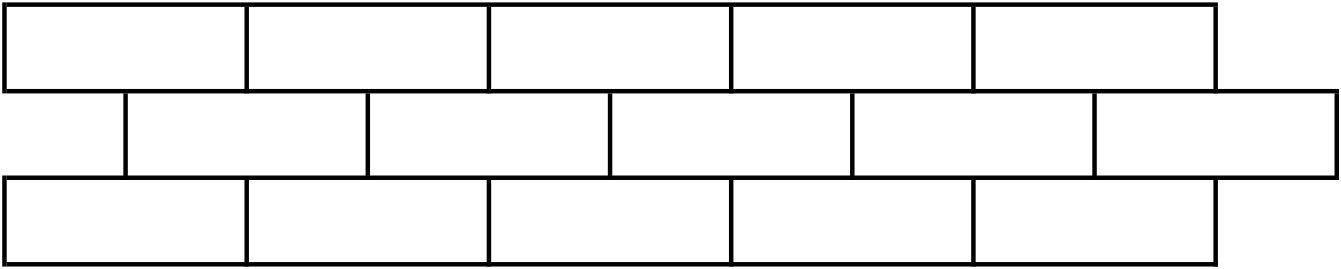
\includegraphics[width=8cm]{brick3x5}
	\end{figure}
	(b) Đếm số cách chọn ra 4 viên gạch, mỗi viên từ 1 hàng trong $4\times5$ viên gạch xếp xen kẽ, sao cho không có 2 viên gạch nào được lấy ra nằm kề nhau.
	\begin{figure}[H]
		\centering
		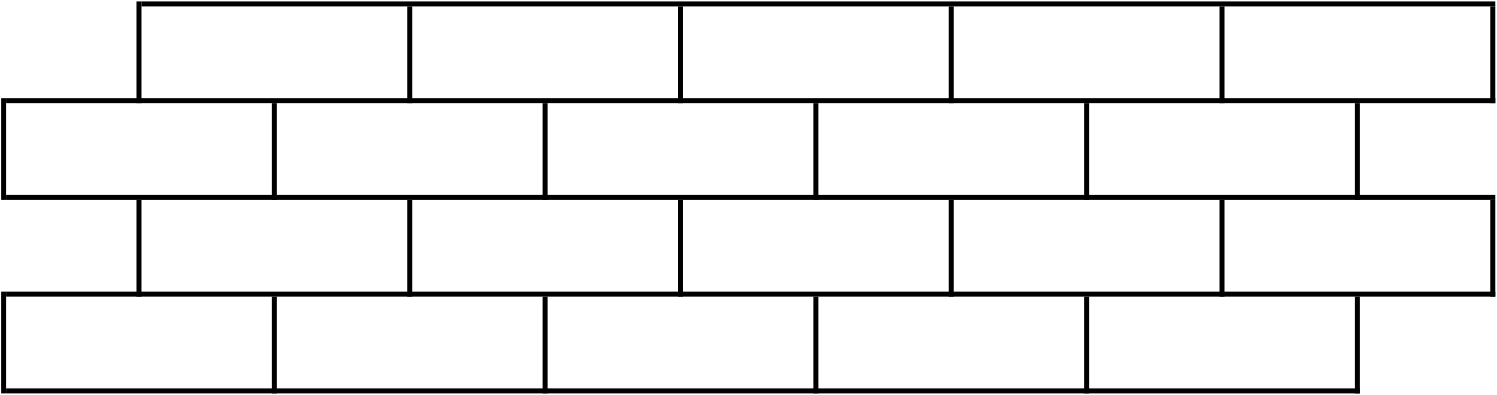
\includegraphics[width=8cm]{brick4x5}
	\end{figure}
	(c) Cho $m,n\in\mathbb{N}^\star$. Đếm số cách chọn ra $m$ viên gạch, mỗi viên từ 1 hàng trong $m\times n$ viên gạch xếp xen kẽ, sao cho không có 2 viên gạch nào được lấy ra nằm kề nhau. (d) Cho $m,n,k\in\mathbb{N}^\star$. Đếm số cách chọn ra $k$ viên gạch, không nhất thiết mỗi viên từ 1 hàng trong $m\times n$ viên gạch xếp xen kẽ, sao cho không có 2 viên gạch nào được lấy ra nằm kề nhau. (e${}^\star$) Mở rộng cho trường hợp $m\times n$ với số gạch mỗi hàng có thể khác nhau, cụ thể là hàng $i$ chứa $a_i\in\mathbb{N}^\star$ viên gạch, $\forall i = 1,\ldots,m$ với 2 trường hợp: (i) Mỗi viên từ 1 hàng. (ii) Lấy $k\in\mathbb{N}^\star$ viên gạch, mỗi hàng có thể lấy nhiều viên.
\end{baitoan}

\begin{nhanxet}[Left-right symmetry -- Đối xứng trái phải]
	Nếu số viên gạch của mỗi hàng bằng nhau \& được sắp xen kẽ như (a) \& (b), thì thứ tự viên gạch đầu tiên từ bên trái của mỗi hàng lồi ra hay thụt vào không quan trọng, vì có thể lấy đối xứng gương trái--phải để chuyển đổi 2 trường hợp đó. Cũng chú ý đến tính đối xứng trên--dưới (top-bottom symmetry).
\end{nhanxet}

\begin{proof}
	Số cách chọn gạch từ 3 hàng, mỗi hàng $n$ viên gạch: $(n - 1)(n - 2)^2 + (n - 1)^2 = (n - 1)(n^2 - 3n + 3)$, $\forall n\in\mathbb{N}^\star$, $n\ge2$. Số cách chọn gạch từ 4 hàng, mỗi hàng $n\in\mathbb{N}^\star$ viên gạch: $(n^2 - 3n + 3)^2$, $\forall n\in\mathbb{N}^\star$, $n\ge2$.
\end{proof}

\begin{itemize}
	\item C++ codes:
	\begin{itemize}
		\item (DKAK): \url{https://github.com/NQBH/advanced_STEM_beyond/blob/main/VMC/C++/brick_DPAK.cpp}.
		\item (NLDK): \url{https://github.com/NQBH/advanced_STEM_beyond/blob/main/VMC/C++/brick_NLDK.cpp}.
	\end{itemize}
\end{itemize}

%------------------------------------------------------------------------------%

\subsection{Permutation group -- Nhóm hoán vị}
\textbf{\textsf{Resources -- Tài nguyên.}}
\begin{enumerate}
    \item \href{https://en.wikipedia.org/wiki/Permutation_group}{Wikipedia{\tt/}permutation group}.
\end{enumerate}
Phần này liên quan đến các khái niệm của Đại Số Trừu Tượng (Abstract Algebra) \& ứng dụng của chúng trong Tổ Hợp \& Lý Thuyết Đồ Thị.

In mathematics, a {\it permutation group} is a \href{https://en.wikipedia.org/wiki/Group_(mathematics)}{group} $G$ whose elements are \href{https://en.wikipedia.org/wiki/Permutation}{permutations} of a given set $M$ \& whose \href{https://en.wikipedia.org/wiki/Group_operation}{group operation} is the composition of permutations in $G$ (which are thought of as \href{https://en.wikipedia.org/wiki/Bijective_function}{bijective functions} from the set $M$ to itself). The group of {\it all} permutations of a set $M$ is the \href{https://en.wikipedia.org/wiki/Symmetric_group}{symmetric group} of $M$, often written as ${\rm Sym}(M)$. The term {\it permutation group} thus means a \href{https://en.wikipedia.org/wiki/Subgroup}{subgroup} of the symmetric group. If $M = [n]$ then ${\rm Sym}(M)$ is usually denoted by $S_n$:
\begin{equation*}
    S_n\coloneqq{\rm Sym}([n]) = {\rm Sym}(\{1,2,\ldots,n\}),\ \forall n\in\mathbb{N}^\star,
\end{equation*}
\& may be called the {\it symmetric group on $n$ letters}.

-- Trong toán học, 1 {\it permutation group} là 1 nhóm $G$ có các phần tử là các hoán vị của 1 tập hợp $M$ cho trước \& có phép toán nhóm là hợp các hoán vị trong $G$ (được coi là các hàm song ánh từ tập hợp $M$ vào chính nó). Nhóm {\it all} permutation của 1 tập hợp $M$ là nhóm đối xứng của $M$, thường được viết là ${\rm Sym}(M)$. Do đó, thuật ngữ {\it permutation group} có nghĩa là 1 nhóm con của nhóm đối xứng. Nếu $M = [n]$ thì ${\rm Sym}(M)$ thường được ký hiệu là $S_n$:
\begin{equation*}
    S_n\coloneqq{\rm Sym}([n]) = {\rm Sym}(\{1,2,\ldots,n\}),\ \forall n\in\mathbb{N}^\star,
\end{equation*}
\& có thể được gọi là {\it nhóm đối xứng trên $n$ chữ cái}.

By \href{https://en.wikipedia.org/wiki/Cayley%27s_theorem}{Cayley's theorem}, every group is \href{https://en.wikipedia.org/wiki/Isomorphic}{isomorphic} to some permutation group.

-- Theo định lý Cayley, mọi nhóm đều đồng cấu với 1 nhóm hoán vị nào đó.

The way in which the elements of a permutation group permute the elements of the set is called its \href{https://en.wikipedia.org/wiki/Group_action_(mathematics)}{group action}. Group actions have applications in the study of \href{https://en.wikipedia.org/wiki/Symmetry}{symmetries}, combinatorics, \& many other branches of mathematics, physics, \& chemistry.

-- Cách mà các phần tử của 1 nhóm hoán vị hoán vị các phần tử của tập hợp được gọi là hành động nhóm của nó. Hành động nhóm có ứng dụng trong nghiên cứu về tính đối xứng, tổ hợp \& nhiều nhánh khác của toán học, vật lý \& hóa học.

%------------------------------------------------------------------------------%

\subsubsection{Basic properties \& terminology of permutation group -- Tính chất cơ bản \& thuật ngữ của nhóm hoán vị}
***

%------------------------------------------------------------------------------%

\subsubsection{Composition of permutations -- the group product}
***

%------------------------------------------------------------------------------%

\section{Problems: Counting -- Bài tập: Đếm}

\begin{baitoan}
	1 lớp có $n\in\mathbb{N}^\star$ sinh viên. Lớp muốn trong bức ảnh có $a\in\mathbb{N}^\star$ ngồi hàng đầu \& $n - a$ sinh viên ngồi hàng sau. Đếm số cách.
\end{baitoan}

\begin{proof}
	Chọn ra $a$ bạn ngồi hàng đầu \& sắp vị trí: có $A_n^a$ cách. Hoán vị $n - a$ bạn còn lại vào hàng sau: có $(n - a)!$ cách. Theo quy tắc nhân, có $A_n^a(n - a)! = \dfrac{n!}{(n - a)!}(n - a)! = n!$ cách.
\end{proof}

\begin{problem}[\cite{Shahriari2022}, p. 2]
	Given $m,n\in\mathbb{N}^\star$, $m\le n$. Count the number of sequences $a_1,a_2,\ldots,a_n$ consisting of $m$ $0$'s \& $n - m$ $1$'s, if no 2 consecutive terms are both $0$'s? Write {\sf C{\tt/}C++, Python} programs to illustrate.
	
	-- Cho $m,n\in\mathbb{N}^\star$, $m\le n$. Đếm số dãy số $a_1,a_2,\ldots,a_n$ gồm $m$ $0$'s \& $n - m$ $1$'s, nếu không có 2 số hạng liên tiếp nào đều là $0$'s? Viết chương trình {\sf C{\tt/}C++, Python} để mô phỏng.
\end{problem}

\begin{proof}
	$C_{n - m + 1}^m$.
	
	C++:
	\begin{verbatim}
		#include<bits/stdc++.h>
		using namespace std;
		
		long long total = 0;
		
		long long nCk(int n, int k) {
			if (k>n||k<0) return 0;
			long long res=1;
			for(int i=1; i<=k; i++) {
				res*=(n-i+1);
				res/=i;
			}
			return res;
		}
		
		void generateSeq(int n, int m, int pos, int last, vector<int>& seq, int cnt0, int cnt1) {
			if (cnt0>m || cnt1>n-m) return;
			if (pos==n) {
				if(cnt0==m && cnt1==n-m) {
					for(int x:seq) cout<<x<<" ";
					cout<<"\n";
					total++;
				}
			}
			
			seq.push_back(1);
			generateSeq(n, m, pos+1, 1, seq, cnt0, cnt1+1);
			seq.pop_back();
			
			if(last!=0) {
				seq.push_back(0);
				generateSeq(n, m, pos+1, 0, seq, cnt0+1, cnt1);
				seq.pop_back();
			}
		}
		
		
		int main() {
			ios_base::sync_with_stdio(0);
			cin.tie(0); cout.tie(0);
			int n, m;
			cin>>n>>m;
			vector<int> seq;
			generateSeq(n, m, 0, -1, seq, 0, 0);
			cout<<"Tong so day hop le: "<<total<<"\n";
			cout<<"(n-m+1)Cm = "<<nCk(n-m+1, m);
		}
	\end{verbatim}
\end{proof}

\begin{problem}[\cite{Shahriari2022}, p. 3]
	Let $f(n)$ be the number of subsets of $[n]$. Prove that $f(n) = 2^n$, $\forall n\in\mathbb{N}^\star$.
\end{problem}

\begin{problem}[\cite{Shahriari2022}, p. 3]
	Assume $n\in\mathbb{N}$, $n\ge2$, people given their $n$ hats to a hat-check person. Let $f(n)$ be the number of ways that the hats can be returned, so that everyone has 1 hat, but no one has their own hat. Prove: (a) $f(n) = n!\sum_{i=0}^n \dfrac{(-1)^i}{i!}$, $\forall n\in\mathbb{N}^\star$. (b) $f(n)$ is the nearest integer to $\dfrac{n!}{e}$.
\end{problem}

\begin{problem}[\cite{Shahriari2022}, p. 3]
	Given $n\in\mathbb{N}^\star$. Let $f(n)$ be the number of subsets of $[n]$ that do not contain 2 consecutive integers. (a) Compute $f(1),f(2),f(3),f(4)$. (b) Prove: $f(n) = f(n - 1) + f(n - 2)$, $\forall n\in\mathbb{N}$, $n\ge3$. (c) Prove:
	\begin{equation*}
		f(n) = \frac{1}{\sqrt{5}}\left(\tau^{n+2} - \overline{\tau}^{n+2}\right),\mbox{ where }\tau = \frac{1 + \sqrt{5}}{2},\ \overline{\tau} = \frac{1 - \sqrt{5}}{2}.
	\end{equation*}
\end{problem}

%------------------------------------------------------------------------------%

\section{Euler candy problem -- Bài toán chia kẹo Euler}

\begin{baitoan}[Euler candy problem -- Bài toán chia kẹo Euler]
	Cho $m,n\in\mathbb{N}^\star$. Xét phương trình nghiệm nguyên
	\begin{equation}
		\label{Euler candy}
		\sum_{i=1}^n x_i = m.
	\end{equation}
	(a) Đếm số nghiệm nguyên dương của phương trình \eqref{Euler candy}. (b) Đếm số nghiệm nguyên không âm của phương trình \eqref{Euler candy}. (c) Đếm số nghiệm nguyên của phương trình
	\begin{equation*}
		\sum_{i=1}^m x_i + \sum_{i=1}^n y_i = p\mbox{ s.t. }\left\{\begin{split}
			x_i&\ge1,\ \forall i\in[m],\\
			y_i&\ge0,\ \forall i\in[n],
		\end{split}\right.
	\end{equation*}
	(d) Đếm số nghiệm nguyên của phương trình
	\begin{equation*}
		\sum_{i=1}^n x_i = m\mbox{ s.t. } x_i\ge m_i,\ \forall i\in[n].
	\end{equation*}
	(e) Đếm số nghiệm nguyên của phương trình
	\begin{equation*}
		\sum_{i=1}^n x_i = m\mbox{ s.t. } m_i\le x_i\le M_i,\ \forall i\in[n].
	\end{equation*}
\end{baitoan}

\begin{proof}
	(a) $C_{m-1}^{n-1}$. (b) $C_{p + n - 1}^{m + n - 1}$. (d) $C_{m + n - 1 - \sum_{i=1}^n m_i}$.
\end{proof}

%------------------------------------------------------------------------------%

\section{Method of mathematical induction \& recurrence -- Phương pháp quy nạp toán học \& truy hồi{\tt/}đệ quy}
{\sf Ideas of method of mathematical induction.} In philosophy \& in the sciences, the inductive method refers to the process of starting with observations \& then looking for general laws \& theories. Mathematical induction -- which we just called {\it induction} -- is quite different. For us, induction is a method of proof. When we have an infinite sequence $\{P_n\}_{n=1}^\infty = P_1,P_2,\ldots$ of (related) mathematical statements that need a proof, then instead of proving each 1 of these statements, we may be able to just prove that whenever 1 of the statements is true, then so is the next statement (i.e., if $P_k$ is true, then so is $P_{k+1}$). If we manage such a feat, then proving $P_1$, the 1st statement, starts a domino effect resulting in all of the statements being true.

-- {\sf Ý tưởng về phương pháp quy nạp toán học.} Trong triết học \& trong khoa học, phương pháp quy nạp đề cập đến quá trình bắt đầu bằng các quan sát \& sau đó tìm kiếm các định luật \& lý thuyết chung. Quy nạp toán học -- mà chúng ta chỉ gọi là {\it quy nạp} -- thì khá khác. Đối với chúng ta, quy nạp là 1 phương pháp chứng minh. Khi chúng ta có 1 chuỗi vô hạn $\{P_n\}_{n=1}^\infty = P_1,P_2,\ldots$ các mệnh đề toán học (có liên quan) cần được chứng minh, thì thay vì chứng minh từng 1 trong số các mệnh đề này, chúng ta có thể chỉ cần chứng minh rằng bất cứ khi nào 1 trong các mệnh đề là đúng, thì mệnh đề tiếp theo cũng vậy (tức là nếu $P_k$ đúng, thì $P_{k+1}$ cũng đúng). Nếu chúng ta thực hiện được kỳ tích như vậy, thì việc chứng minh $P_1$, mệnh đề đầu tiên, sẽ bắt đầu 1 hiệu ứng domino khiến tất cả các mệnh đề đều đúng.

{\sf Intuition.} A sequence of {\it consecutive} pieces of domino falling.

-- {\sf Trực giác.} Phương pháp quy nạp toán học hoạt động như cách 1 chuỗi các quân cờ domino {\it liên tiếp} rơi xuống sau khi đẩy ngã quân domino đầu tiên (1 quân domino bất kỳ bị ngã sẽ khiến quân domino tiếp theo nó bị ngã).

{\sf Principle of Mathematical Induction.} Given an infinite sequence of propositions $\{P_n\}_{n=1}^\infty = P_1,P_2,\ldots,P_n,\ldots$, in order to prove that all of them are true, it is enough to show 2 things:
\begin{itemize}
	\item The base case: $P_1$ is true.
	\item The inductive step: For all $k\in\mathbb{N}^\star$, if $P_k$ is true, then so is $P_{k+1}$.
\end{itemize}

\begin{remark}
	1 drawback of mathematical induction: to use it, you already have to know the pattern \& the answer. Mathematical induction -- unlike the inductive method in science -- does not help in finding the pattern. 1 strength of induction: it allows you to use $P_k$ to prove $P_{k+1}$. This is a big advantage -- it almost seems like cheating -- since often $P_k$ looks very much like $P_{k+1}$.
	
	-- 1 nhược điểm của quy nạp toán học: để sử dụng nó, bạn phải biết mô hình \& câu trả lời. Quy nạp toán học -- không giống như phương pháp quy nạp trong khoa học -- không giúp tìm ra mô hình. 1 điểm mạnh của quy nạp: nó cho phép bạn sử dụng $P_k$ để chứng minh $P_{k+1}$. Đây là 1 lợi thế lớn -- gần giống như gian lận -- vì thường thì $P_k$ trông rất giống $P_{k+1}$.
\end{remark}

\begin{baitoan}
	Chứng minh: (a) {\rm(Tổng của $n$ số nguyên dương đầu tiên, $n$ số nguyên lẻ đầu tiên, $n$ số nguyên dương chẵn đầu tiên)} $\sum_{i=1}^n i = \dfrac{n(n + 1)}{2}$, $\sum_{i=1}^n (2i - 1) = n^2$, $\sum_{i=1}^n 2i = n(n + 1)$, $\forall n\in\mathbb{N}^\star$. (b) {\rm(Tổng bình phương của $n$ số nguyên dương đầu tiên, $n$ số nguyên lẻ đầu tiên, $n$ số nguyên dương chẵn đầu tiên)} $\sum_{i=1}^n i^2 = \dfrac{n(n + 1)(2n + 1)}{6}$, $\sum_{i=1} (2i - 1)^2,\sum_{i=1}^n (2i)^2$, $\forall n\in\mathbb{N}^\star$. (c) $\sum_{i=1}^n i^3 = \left(\sum_{i=1}^n i\right)^2 = \dfrac{n^2(n + 1)^2}{4}$, $\forall n\in\mathbb{N}^\star$. (d) Tìm cách tính $S(n,k)\coloneqq\sum_{i=1}^n i^k$, $\forall n,k\in\mathbb{N}^\star$. (e) Tính , $\forall n\in\mathbb{N}^\star$. (f) Tính $\sum_{i=1} (2i - 1)^3,\sum_{i=1}^n (2i)^3$, $\forall n\in\mathbb{N}^\star$. () $\sum_{i=1}^n \dfrac{1}{i(i + 1)} = \dfrac{n}{n + 1}$, $\forall n\in\mathbb{N}^\star$. () $\sum_{i=1}^n \dfrac{1}{\sqrt{i} + \sqrt{i + 1}} = \sqrt{n + 1} - 1$, $\forall n\in\mathbb{N}^\star$. () $\prod_{i=1}^n \dfrac{i^3 - 1}{i^3 + 1} = \dfrac{2(n^2 + n + 1)}{3n(n + 1)}$, $\forall n\in\mathbb{N}^\star$.
\end{baitoan}
See, e.g., \href{https://en.wikipedia.org/wiki/Ring_of_integers}{Wikipedia{\tt/}ring of integers}.

\begin{baitoan}
	Cho $m\in\mathbb{N}^\star$ là 1 số không chính phương. Chứng minh: (a) $\exists A,B\in\mathbb{N}^\star$ s.t. $(a + b\sqrt{m})^n = A + B\sqrt{m}$, $\forall n\in\mathbb{N}^\star$. (b) $\exists A,B\in\mathbb{N}^\star$ s.t. $(a - b\sqrt{m})^n = A - B\sqrt{m}$, $\forall n\in\mathbb{N}^\star$.
\end{baitoan}

\begin{baitoan}
	Chứng minh: (a) $(a + 1)^n - an - 1\divby n^2$, $\forall n\in\mathbb{N}^\star$, $\forall a\in\mathbb{Z}$. (b) $(a + 1)^n - \dfrac{n(n - 1)}{2}a^2 - an - 1\divby n^3$, $\forall a\in\mathbb{Z}$.
\end{baitoan}

\begin{problem}[\cite{Shahriari2022}, P1.1.2, p. 10]
	Prove: (a) {\rm(Formula of triangle numbers)} $\sum_{i=1}^n i = \dfrac{n(n + 1)}{2}$, $\forall n\in\mathbb{N}^\star$. (b) {\rm(Partial sums of geometric sequences)}
	\begin{equation*}
		S_n(a)\coloneqq\sum_{i=0}^n a^i = \left\{\begin{split}
			&n + 1&&\mbox{if } a = 1,\\
			&\dfrac{a^{n+1} - 1}{a - 1}&&\mbox{if } a\ne1,
		\end{split}\right.\ \forall n\in\mathbb{N}^\star.
	\end{equation*}
	(c) Compute $1 + \sum_{i=1}^n ii!$, $\forall n\in\mathbb{N}^\star$. (d) Compute $3\sum_{i=1}^n i(i + 1)$, $\forall n\in\mathbb{N}^\star$. (e) Compute $\sum_{i=1}^n i^2$, $\forall n\in\mathbb{N}^\star$.
\end{problem}
{\sf Hint.} (ii) Compute $aS_n(a) - S_n(a)$.

\begin{remark}
	The sequence of integers $\left\{\dfrac{n(n + 1)}{2}\right\}_{n=1}^\infty$ are called {\rm triangle numbers} since they count the number of dots in progressively larger triangles.
\end{remark}

\begin{baitoan}[\cite{Shahriari2022}, p. 6]
	Trên 1 tờ giấy vuông lớn, vẽ $n\in\mathbb{N}^\star$ các đường thẳng bắt đầu từ 1 cạnh của hình vuông \& kết thúc ở cạnh còn lại. Mỗi 2 đường thẳng cắt nhau nhưng không có 3 (hoặc nhiều hơn) đường thẳng nào đi qua cùng 1 điểm. Giả sử $f(n)$ là số vùng mà các đường thẳng chia tờ giấy. Tính 1 số giá trị của $f(n)$ \& dự đoán công thức chung của nó.
\end{baitoan}

\begin{problem}[\cite{Shahriari2022}, p. 6]
	You have $100$ briefcases numbered $1$ through $100$. For any $n\in\mathbb{N}^\star$, if a briefcase numbered $n$ holds cash, then so does the briefcase numbered $n + 3$. You open up briefcase numbered $55$ \& it has a stuffed animal in it. Can you conclude anything about any of the other briefcases?
\end{problem}

\begin{baitoan}[\cite{Shahriari2022}, p. 6]
	Bạn có $100$ cặp được đánh số từ $1$ đến $100$. Đối với bất kỳ $n\in\mathbb{N}^\star$ nào, nếu 1 cặp được đánh số $n$ đựng tiền mặt, thì cặp được đánh số $n + 3$ cũng vậy. Bạn mở cặp được đánh số $55$ \& bên trong có 1 con thú nhồi bông. Bạn có thể kết luận điều gì về bất kỳ cặp nào khác không?	
\end{baitoan}

%------------------------------------------------------------------------------%

\section{Principle of strong induction -- Nguyên lý quy nạp mạnh}
Given an infinite sequence of propositions $\{P_n\}_{n=1}^\infty = P_1,P_2,\ldots,P_n,\ldots$ in order to demonstrate that all of them are true, it is enough to know 2 things:
\begin{itemize}
	\item The base case: $P_1$ is true.
	\item The inductive step: $\forall k\in\mathbb{N}^\star$, if $P_1,P_2,\ldots,P_k$ are true, then so is $P_{k+1}$.
\end{itemize}

%------------------------------------------------------------------------------%

\section{Fibonacci \& Lucas numbers}

\begin{definition}[Fibonacci sequences]
	{\sf Fibonacci sequences} are defined by
	\begin{equation*}
		\left\{\begin{split}
			F_0 &= 0,\ F_1 = 1,\\
			F_n &= F_{n - 1} + F_{n - 2},\ \forall n\in\mathbb{N},\,n\ge2.
		\end{split}\right.
	\end{equation*}
\end{definition}

\begin{baitoan}[Fibonacci numbers -- Số Fibonacci]
	Tính dãy số Fibonacci bằng: (a) Truy hồi $O(a^n)$ với $a\approx1.61803$. (b) Quy hoạch động $O(n)$. (c) Quy hoạch động cải tiến. Trong mỗi thuật toán, tính cụ thể số lần gọi hàm tính $F(i)$, với $i = 0,1,\ldots,n$, số phép cộng đã thực hiện. Tính time- \& space complexities.
\end{baitoan}
C++: \url{https://github.com/NQBH/advanced_STEM_beyond/blob/main/OLP_ICPC/C++/Fibonacci.cpp}.
\begin{verbatim}
	#include <iostream>
	using namespace std;
	const long nMAX = 10000;
	
	long fib(long i) {
		if (i == 1 || i == 2)
		return 1;
		else
		return fib(i - 1) + fib(i - 2);
	}
	
	// \cite{Thu_Phuong_Tien_Triet_Phuong_KTLT}, p. 443
	long fib_recurrence(long n) {
		long ans, Fn_1, Fn_2;
		if (n <= 2)
		ans = 1;
		else {
			Fn_1 = fib_recurrence(n - 1);
			Fn_2 = fib_recurrence(n - 2);
			ans = Fn_1 + Fn_2;
		}
		return ans;
	}
	
	// \cite{Thu_Phuong_Tien_Triet_Phuong_KTLT}, p. 443
	long fib_dynamic(long n) {
		long F[nMAX + 1];
		F[0] = 0;
		F[1] = F[2] = 1;
		for (int i = 2; i <=n; ++i)
		F[i] = F[i - 1] + F[i - 2];
		return F[n];
	}
	
	// \cite{Thu_Phuong_Tien_Triet_Phuong_KTLT}, p. 443
	long fib_dynamic_improved(long n) {
		long lastF = 1, F = 1;
		int i = 1;
		while (i < n) {
			F += lastF;
			lastF = F - lastF;
			++i;
		}
		return F;
	}
	
	int main() {
		long n, i;
		cin >> n;
		cout << "Fibonacci sequence of length " << n << ":\n";
		
		for (i = 0; i <= n; ++i)
		cout << fib(i) << " ";
		cout << "\n";
		
		for (i = 0; i <= n; ++i)
		cout << fib_recurrence(i) << " ";
		cout << "\n";
		
		for (i = 0; i <= n; ++i)
		cout << fib_dynamic(i) << " ";
		cout << "\n";
		
		for (i = 0; i <= n; ++i)
		cout << fib_dynamic_improved(i) << " ";
		cout << "\n";
	}
\end{verbatim}

\begin{definition}[Lucas sequences]
	The sequence of {\sf Lucas numbers} are defined by
	\begin{equation*}
		\left\{\begin{split}
			L_0 &= 2,\ L_1 = 1,\\
			L_n &= L_{n - 1} + L_{n - 2},\ \forall n\in\mathbb{N},\,n\ge2.
		\end{split}\right.
	\end{equation*}
\end{definition}

%------------------------------------------------------------------------------%

\section{Recurrence Relations -- Quan hệ truy hồi{\tt/}hồi quy{\tt/}đệ quy}
\textbf{\textsf{Resources -- Tài nguyên.}}
\begin{enumerate}
	\item \href{https://en.wikipedia.org/wiki/Recurrence_relation}{Wikipedia{\tt/}recurrence relation}.
    
	\item \cite{Shahriari2022}. {\sc Shahriar Shahriari}. {\it An Invitation To Combinatorics}. Sect. 1.3: Recurrence Relations.
\end{enumerate}

\begin{problem}[\cite{Shahriari2022}, Warm-Up 1.8, p. 19]
	We have $n$ dollars. Every day we buy exactly 1 of the following products: Mustard \$1, Mint \$2, Marjoram \$2. Let $f(n)$ be the number of possible ways of spending all the money. E.g., $f(3) = 5$, since the possible ways of spending \$3 are: Mustard-Mustard-Mustard, Mustard-Mint, Mustard-Marjoram, Mint-Mustard, \& Marjoram-Mustard. (a) Compute $f(1),f(2)$. (b) Which one(s) (if any) of the following are true? (i) $f(n) = 2f(n - 1) + f(n - 3)$. (ii) $f(n) = f(n - 1) + \frac{n - 1}{2}[3 + (-1)^n]$. (iii) $f(n) = f(n - 1) + 2f(n - 2)$. (d) $f(n) = 2f(n - 1) - f(n - 2)$. Give adequate \& complete reasoning for your answer.
\end{problem}

\begin{proof}[Solution]
	(a) $f(1) = 1$ since we can only 1 Mustard. $f(2) = 3$ since we can buy Mustard-Mustard, Mint, or Marjoram.
	\item(b) Suppose we have $n$\$. On the last day, if we use \$1 to buy Mustard, then the number of possible ways of spending all \$$(n - 1)$ is $f(n - 1)$. Otherwise, on the last day, if we use \$2 to buy either Mint or Marjoram, then the number of possible ways of spending all \$$(n - 2)$ is $f(n - 2)$. Combining both cases yields $f(n) = f(n - 1) + 2f(n - 2)$, $\forall n\in\mathbb{N}$, $n\ge3$.
\end{proof}
You are asked to find a formula for $f(n)$ but not the usual kind of formula of $f(n)$ in terms of $n$. What you are asked to do is to find a formula that gives $f(n)$ in terms of $f(n - 1),f(n - 2)$, \& possibly other values of the $f$ function. Such a relation is called a {\it recurrence relation} \&, while it does not give a direct closed formula for $f(n)$, it provides an efficient way for computing specific values of the function $f$. 

\begin{problem}
	Solve the above problem if the prices of these items are changed as follows: (a) Mustard \$1, Mint \$2, \& Marjoram \$3. (b) Mustard \$$a$, Mint \$$b$, \& Marjoram \$$c$ with $a,b,c\in\mathbb{N}^\star$. 
\end{problem}

\begin{problem}[\cite{Shahriari2022}, p. 6]
	On a large square piece of paper, draw $n\in\mathbb{N}^\star$ straight lines that start from 1 side of the square \& end on another side. Each 2 of the lines intersect but no 3 (or more) lines go through the same point. Let $f(n)$ be the number of regions which the lines split the piece of paper. Compute some values of $f(n)$ \& predict its general formula.
	
	-- Trên 1 tờ giấy vuông lớn, vẽ $n\in\mathbb{N}^\star$ các đường thẳng bắt đầu từ 1 cạnh của hình vuông \& kết thúc ở cạnh còn lại. Mỗi 2 đường thẳng cắt nhau nhưng không có 3 (hoặc nhiều hơn) đường thẳng nào đi qua cùng 1 điểm. Giả sử $f(n)$ là số vùng{\tt/}miền mà các đường thẳng chia tờ giấy. Tính 1 số giá trị của $f(n)$ \& dự đoán công thức chung của nó.
\end{problem}

\begin{question}
	How do we know that the number of regions does not depend on the configuration of the lines? Maybe if we draw the lines in a different relation to each other, the number of regions will change.
	
	-- Làm sao chúng ta biết được số lượng vùng không phụ thuộc vào cấu hình của các đường? Có thể nếu chúng ta vẽ các đường theo 1 mối quan hệ khác với nhau, số lượng vùng sẽ thay đổi.
\end{question}

\begin{proof}[Giải]
	Let $f(n)$ denote the number of regions created by $n\in\mathbb{N}^\star$ straight lines assuming that each pair of lines intersects \& no 3 lines go through the same point (đồng quy). $f(1) = 2,f(2) = 4,f(3) = 7$. Instead of trying to find a formula for $f(n)$ or even trying to prove that $f(n)$ is independent of the position of the lines, we try to determine $f(n)$ in terms of $f(n - 1)$. Not only will this allow us to inductively start with $f(1)$ \& $f(2)$ \& find other values of $f(n)$, but it could also show that $f(n)$ is well defined. We do a thought experiment. Assume that $n - 1$ straight lines split the plane into $f(n - 1)$ regions. How many additional regions are created when we add 1 more line? If we just zoom onto this new line \& follow its path, it will start from 1 side of the square, 1 by 1 cross the $n - 1$ other lines, \& end at another side of the square. Hence, it will go through $n$ regions created by the original $n - 1$ lines. (The 1st region is the one our line is traversing before it hits the 1st line, the 2nd region is between the 1st \& the 2nd, \& so on until the $(n - 1)$th region -- i.e., between the $(n - 2)$th \& $(n - 1)$th lines. Finally, the $n$th region is after the $(n - 1)$th line.) Our line line will split each of these $n$ regions into 2, \& as a result will add $n$ regions to what was there before, hence $f(n) = f(n - 1) + n$, $\forall n\in\mathbb{N}^\star$. This relationship also proves that $f(n)$ does not depend on the configuration of the lines, \& t hat it is well defined. (After all, no matter how the lines are configured, if $f(n - 1)$ is well-defined, then $f(n)$ must be $f(n - 1) + n$. Since $f(1)$ is well defined, by induction all values of $f(n)$ are well defined.) Note that we could have even started with the case $n = 0$. Use mathematical induction to obtain $f(n) = 1 + \frac{n(n + 1)}{2}$, $\forall n\in\mathbb{N}$ (just 1 more than the triangle numbers). Thus $f(100) = 1 + \frac{100\cdot101}{2} = 5051$.
\end{proof}

\begin{remark}[A common approach to some combinatorial problems, \cite{Shahriari2022}, Rmk. 1.11, p. 22]
	Often a given combinatorial problem is an instance of a sequence of problems indexed by $n\in\mathbb{N}^\star$, where $n$ is a natural parameter for the problem. If we let $f(n)$ denote the answer to the $n$th instance of our problem, ideally we may want a closed-form formula for $f(n)$. Sometimes, we can find a ``recurrence relation'' for $f$, i.e., finding a formula for $f(n)$ in terms of $f(n - 1),f(n - 2),\ldots$, e.g., $f(n) = f(n - 1) + f(n - 2)$, the defining recurrence relation for the sequence of Pi\.{n}gala--Fibonacci numbers. Usually, the recurrence relation itself is not proved by induction. Rather, we often use a ``thought experiment''. What are the possibilities for the ``1st'' or ``last'' step of the problem? 
	
	After we have a recurrence relation \& a few base cases, we can easily generate data \& record many values for $f(n)$. At this point, there are a number of possible approaches:
	\begin{itemize}
		\item Use a simple computer program to find any particular value of $f(n)$ that you need.
		\item Look at the values of $f(n)$ for small $n$ \& try to guess the pattern. If your guess is correct, sometimes you can translate it to a closed formula, \& often you can prove your conjecture using induction. You can use the recurrence relation in your proof by induction. Recurrence relations are especially suited to help with proofs by induction.
		\item Some classes of recurrence relations (e.g., so-called linear recurrence relations) can be solved systematically.
		\item Sometimes you can ``unwind'' the recurrence relation.
		\item Sometimes you can use ``generating functions'' to get information about the sequence $\{f(n)\}_{n=0}^\infty$.
	\end{itemize}
	Guessing the pattern from the starting values of an infinite sequence is not easy. For 1 thing, there are many distinct infinite sequences that agree in the 1st few terms -- after all, there are not that many very small integers, \&, in contrast, there are many infinite sequences of integers. If you have the beginning of a sequence of numbers, \& are wondering what the pattern could be, 1 very fun tool is the \emph{Online Encyclopedia of Integer Sequences} at \url{https://oeis.org/}
\end{remark}

\begin{question}[1st step vs. last step]
	When should we focus on the 1st step of a problem to establish a recurrence relation? When on the last step?
	
	-- Khi nào chúng ta nên tập trung vào bước đầu tiên của 1 bài toán để thiết lập mối quan hệ lặp lại? Khi nào là bước cuối cùng?
\end{question}
A recurrence, for the integer valued function $f$, of the form $f(n) = \sum_{i=1}^k \alpha_if(n - i) + g(n) = \alpha_1f(n - 1) + \alpha_2f(n - 2) + \cdots + \alpha_kf(n - k) + g(n)$, where $\alpha_i$ are scalars, $\forall i\in[k]$, \& $g$ is a function of $n$, is called a {\it linear recurrence relation}. If you are lucky \& the recurrence relation is linear, then the most fruitful method is to 1st ignore the initial conditions \& find, basically by an educated guess, a set of functions that satisfy the recurrence relation, \& then use the initial conditions to choose a function that satisfies both the initial conditions \& the recurrence relation. The key observation -- which will be used often -- is that if 2 functions have the same initial values \& satisfy the same recurrence conditions, then they will have to be the same for all later inputs. See \cite[Sect. 1.4]{Shahriari2022} where both linear recurrence relations \& the idea of unwinding a recurrence relation were explored.

\begin{baitoan}
	Cho $m,n\in\mathbb{N}^\star$ cố định. Đếm số nghiệm nguyên dương của phương trình $\sum_{i=1}^d x_i = n$ trong đó $x_i$ chỉ có thể nhận $1$ trong $m$ giá trị cho trước $a_1,a_2,\ldots,a_m$, i.e., $x_i\in\{a_1,\ldots,a_m\}$, $\forall i\in[d]$, $d\in\mathbb{N}^\star$ có thể thay đổi.
\end{baitoan}

\begin{remark}[\cite{Shahriari2022}, Rmk. 1.11, p. 22]
	The problems in this section are ment to give you experience in setting up a recurrence relation for a counting problem. This skill will be used throughout the book. In some problems, you are also asked to use the recurrence relation, generate some data, guess the pattern, \& prove it by induction. The 2 techniques: solving linear recurrences \& unwinding when applicable give a better alternative to ``guess-the-pattern'' of the current section. Yet a 4th method -- using generating functions -- will be discussed in \cite[Chap. 9]{Shahriari2022}.
\end{remark}

%------------------------------------------------------------------------------%

\subsection{Problems: Recurrence relation -- Bài tập: Quan hệ hồi quy}

\begin{problem}[\cite{Shahriari2022}, P1.3.1, p. 22]
	We are given the following recurrence relation $a_1 = 2$, $a_n = 3a_{n-1} + 2$ for $n\in\mathbb{N},n\ge2$. Find the values of $a_n$ for small $n$. Do you see a pattern? Make a conjecture. Prove your conjecture using induction.
    
    -- Chúng ta được cho hệ thức đệ quy sau $a_1 = 2$, $a_n = 3a_{n-1} + 2$ đối với $n\in\mathbb{N},n\ge2$. Tìm các giá trị của $a_n$ đối với $n$ nhỏ. Bạn có thấy 1 mô hình không? Đưa ra 1 phỏng đoán. Chứng minh phỏng đoán của bạn bằng cách sử dụng quy nạp.
\end{problem}

\begin{problem}[\cite{Shahriari2022}, P1.3.2, p. 22]
	Let $n\in\mathbb{N}$. We know that $f(0) = -3$, \& $f(n) = 3f(n - 1) + 10$, $\forall n\in\mathbb{N}^\star$. Generate some data, \& use the data to conjecture a closed formula for $f(n)$. Prove your conjecture using induction.
    
    -- Cho $n\in\mathbb{N}$. Ta biết rằng $f(0) = -3$, \& $f(n) = 3f(n - 1) + 10$, $\forall n\in\mathbb{N}^\star$. Tạo 1 số dữ liệu, \& sử dụng dữ liệu để suy ra công thức đóng cho $f(n)$. Chứng minh suy đoán của bạn bằng quy nạp.
\end{problem}

\begin{problem}[\cite{Shahriari2022}, P1.3.3, p. 22]
	Let $h_n$ denote the number of ways of covering a $2\times n$ array with $1\times n$ dominoes. Find $h_1,h_2,h_3$, \& a recurrence relation for $h_n$. Use these to find $h_8$.
    
    -- Giả sử $h_n$ biểu thị số cách phủ mảng $2\times n$ bằng $1\times n$ domino. Tìm $h_1,h_2,h_3$, \& 1 quan hệ đệ quy cho $h_n$. Sử dụng chúng để tìm $h_8$.
\end{problem}

\begin{problem}[\cite{Shahriari2022}, P1.3.4, pp. 22--23]
	Let $n\in\mathbb{N}^\star$. Consider a $1\times n$ strip of cardboard. We have (a large number of) $3$ types of pieces: $1\times2$ red pieces, $1\times4$ yellow pieces, \& $1\times4$ blue pieces. Let $f(n)$ be the number of ways that we can title the strip of cardboard with our pieces. E.g., $f(3) = 0$ since you cannot tile a $1\times3$ board with the available pieces, while $f(6) = 5$ since the possibilities are {\tt YR, RY, RB, BR, RRR}. Find $f(14)$. (Give an actual number.)
    
    -- Cho $n\in\mathbb{N}^\star$. Xét 1 dải bìa cứng $1\times n$. Chúng ta có (1 số lượng lớn) $3$ loại mảnh: $1\times2$ mảnh đỏ, $1\times4$ mảnh vàng, \& $1\times4$ mảnh xanh. Cho $f(n)$ là số cách chúng ta có thể đặt tên cho dải bìa cứng bằng các mảnh của mình. Ví dụ, $f(3) = 0$ vì bạn không thể xếp 1 bảng $1\times3$ bằng các mảnh có sẵn, trong khi $f(6) = 5$ vì các khả năng là {\tt YR, RY, RB, BR, RRR}. Tìm $f(14)$. (Nêu 1 số thực tế.)
\end{problem}

\begin{problem}[\cite{Shahriari2022}, P1.3.5, p. 23]
	Generations of Indian commentators, apparently beginning with Pingala in the 3rd to 2nd century BCE, were interested in the number of rhythmic patterns having a total of $n\in\mathbb{N}^\star$ beats. Assuming that we use only $1$-beat \& $2$-beat rhythms, how many different patterns can we make that have a total of $n$ beats? E.g., if $n = 4$, we can have $2 - 2,2 - 1 - 1,1 - 2 - 1,1 - 1 - 2,1 - 1 - 1 - 1$ for a total of $5$ possibilities. If we denote the answer by $r(n)$, then find a recurrence relation for $r(n)$. Is $r(n)$ related to the Pingala--Fibonacci numbers?
    
    -- Nhiều thế hệ nhà bình luận Ấn Độ, rõ ràng bắt đầu từ Pingala vào thế kỷ thứ 3 đến thế kỷ thứ 2 trước Công nguyên, đã quan tâm đến số lượng các mẫu nhịp điệu có tổng cộng $n\in\mathbb{N}^\star$ nhịp. Giả sử rằng chúng ta chỉ sử dụng nhịp điệu $1$-nhịp \& $2$-nhịp, thì chúng ta có thể tạo ra bao nhiêu mẫu nhịp điệu khác nhau có tổng cộng $n$ nhịp? Ví dụ, nếu $n = 4$, chúng ta có thể có $2 - 2,2 - 1 - 1,1 - 2 - 1,1 - 1 - 2,1 - 1 - 1 - 1$ với tổng cộng $5$ khả năng. Nếu chúng ta biểu thị câu trả lời bằng $r(n)$, thì hãy tìm 1 hệ thức đệ quy cho $r(n)$. $r(n)$ có liên quan đến dãy số Pingala--Fibonacci không?
\end{problem}

\begin{problem}[\cite{Shahriari2022}, P1.3.6, p. 23]
	In his 1202 book {\rm Liber Abaci}, {\sc Leonardo} of Pisa (known as {\sc Fibonacci} since the 19th century) poses the following problem:
    \begin{quotation}
        A certain man put a pair of rabbits in a place surrounded on all sides by a wall. How many pairs of rabbits can be produced from that pair in a year if it is supposed that every month each pair begets a new pair which from the 2nd month on becomes productive?
    \end{quotation}
    Give a solution. Is this related to the Pingala--Fibonacci numbers? How?
    
    -- Trong cuốn sách năm 1202 của mình {\rm Liber Abaci}, {\sc Leonardo} xứ Pisa (được biết đến với tên {\sc Fibonacci} từ thế kỷ 19) đã đặt ra vấn đề sau:
    \begin{quotation}
        Một người đàn ông nào đó đặt 1 cặp thỏ vào 1 nơi được bao quanh bởi 1 bức tường ở mọi phía. Có bao nhiêu cặp thỏ có thể được tạo ra từ cặp đó trong 1 năm nếu giả sử rằng mỗi tháng, mỗi cặp lại sinh ra 1 cặp mới \& từ tháng thứ 2 trở đi, cặp này sẽ sinh sản?
    \end{quotation}
    Đưa ra giải pháp. Điều này có liên quan đến dãy số Pingala--Fibonacci không? Bằng cách nào?
\end{problem}

\begin{problem}[\cite{Shahriari2022}, P1.3.7, p. 23]
	Assume that, for $n\ge3$, the sequence $\{a_n\}_{n=1}^\infty$ satisfies the recurrence relation $a_n = a_{n-1} + a_{n-2}$. Assume further that we know that $a_2 = 3,a_{50} = 300$. Find $\sum_{i=1}^{48}$ \& justify your answer.
    
    -- Giả sử rằng, với $n\ge3$, dãy $\{a_n\}_{n=1}^\infty$ thỏa mãn hệ thức đệ quy $a_n = a_{n-1} + a_{n-2}$. Giả sử thêm rằng chúng ta biết rằng $a_2 = 3,a_{50} = 300$. Tìm $\sum_{i=1}^{48}$ \& chứng minh câu trả lời của bạn.
\end{problem}

\begin{problem}[\cite{Shahriari2022}, P1.3.8, p. 23]
	You work at a car dealership that sells $3$ models: A pickup truck, an SUV, \& a compact hybrid. Your job is to park the vehicles in a row. The pickup trucks \& the SUV take up $2$ spaces while the hybrid takes up $1$ space. Let $n\in\mathbb{N}^\star$ \& let $f(n)$ be the number of ways of arranging vehicles in exactly $n$ spaces. Find a recurrence relation for $f(n)$ \& use it to find $f(10)$, the number of ways of arranging vehicles if you have $10$ parking spaces.
    
    -- Bạn làm việc tại 1 đại lý ô tô bán $3$ mẫu xe: Một xe bán tải, 1 xe SUV, \& 1 xe hybrid nhỏ gọn. Công việc của bạn là đỗ những chiếc xe này thành 1 hàng. Xe bán tải \& xe SUV chiếm $2$ chỗ trong khi xe hybrid chiếm $1$ chỗ. Giả sử $n\in\mathbb{N}^\star$ \& giả sử $f(n)$ là số cách sắp xếp xe trong đúng $n$ chỗ. Tìm 1 hệ thức đệ quy cho $f(n)$ \& sử dụng nó để tìm $f(10)$, số cách sắp xếp xe nếu bạn có $10$ chỗ đỗ xe.
\end{problem}

\begin{problem}[\cite{Shahriari2022}, P1.3.9, p. 23]
	Continuing with the assumptions \& the notation of Problem P1.3.8. (a) Find $f(1),\ldots,f(5)$. (b) Find \& prove a $1$-step recurrence relation for $f(n)$ (i.e., one that only depends on $f(n - 1)$). (c) Find \& prove a formula for $f(n)$ of the form $f(n) = \frac{1}{?}(2^{n+1} + ?)$.
    
    -- Tiếp tục với các giả định \& ký hiệu của Bài toán P1.3.8. (a) Tìm $f(1),\ldots,f(5)$. (b) Tìm \& chứng minh 1 quan hệ đệ quy $1$-bước cho $f(n)$ (tức là 1 quan hệ chỉ phụ thuộc vào $f(n - 1)$). (c) Tìm \& chứng minh 1 công thức cho $f(n)$ có dạng $f(n) = \frac{1}{?}(2^{n+1} + ?)$.
\end{problem}

\begin{problem}[\cite{Shahriari2022}, P1.3.10, pp. 23--24]
	At a dinner party on the spaceship Enterprise, $3$ life forms are present: Human, Klingons, \& Romulans. The dinner table is a long $1\times n$ board, \& the life forms sit on 1 side of it, next to one another. From each life form there are $> n$ individuals present, \& so only a total of $n$ sit at the table. The only problem is that no $2$ humans want to sit next to each other\footnote{NQBH: Damn these human beings!}. Let $h_n$ denote the number of different ways that $n$ individuals can be seated at the dinner table. Assume that all humans look alike, as do all Klingons \& all Romulans. (a) What is $h_1,h_2$? (b) Which one(s)  (if any) of the following are true, \& which are false? (i) $h_n = 3h_{n-1} - h_{n-2}$. (ii) $h_n = 2h_{n-1} + 2h_{n-2}$. (iii) $h_n = 3h_{n-1} - (n - 1)!$. (iv) $h_n = h_{n-1} + 3h_{n-2} + 2h_{n-3}$. Give adequate \& complete reasoning for your answers.
    
    -- Tại 1 bữa tiệc tối trên tàu vũ trụ Enterprise, có $3$ dạng sống hiện diện: Con người, người Klingon, \& Romulan. Bàn ăn là 1 tấm ván dài $1\times n$, \& các dạng sống ngồi ở 1 phía của bàn, cạnh nhau. Từ mỗi dạng sống có $> n$ cá thể hiện diện, \& do đó chỉ có tổng cộng $n$ ngồi vào bàn. Vấn đề duy nhất là không có $2$ con người nào muốn ngồi cạnh nhau\footnote{NQBH: Chết tiệt bọn người này!}. Giả sử $h_n$ biểu thị số cách khác nhau để $n$ cá nhân có thể ngồi vào bàn ăn. Giả sử rằng tất cả con người đều giống nhau, giống như tất cả người Klingon \& tất cả người Romulan. (a) $h_1,h_2$ là gì? (b) Trong các câu sau, câu nào (nếu có) là đúng, \& câu nào là sai? (i) $h_n = 3h_{n-1} - h_{n-2}$. (ii) $h_n = 2h_{n-1} + 2h_{n-2}$. (iii) $h_n = 3h_{n-1} - (n - 1)!$. (iv) $h_n = h_{n-1} + 3h_{n-2} + 2h_{n-3}$. Đưa ra lý lẽ \& đầy đủ cho câu trả lời của bạn.
\end{problem}

\begin{problem}[\cite{Shahriari2022}, P1.3.11, p. 24]
	Using only the digits $1,2,3$, how many integers can you construct in a way that the sum of the digits is $9$? Examples would be $333,1323,2133,22221$.
    
    -- Chỉ sử dụng các chữ số $1,2,3$, bạn có thể tạo ra bao nhiêu số nguyên sao cho tổng các chữ số bằng $9$? Ví dụ: $333,1323,2133,22221$.
\end{problem}

\begin{problem}[\cite{Shahriari2022}, P1.3.12, p. 24]
	I have $12$ identical irises \& $4$ distinct flowerpots. All the irises are to be planted, \& I want to plant $2,3$, or $4$ irises in each pot. I am interested in finding out the number of ways that this can be done. We 1st generalize the question. Given $n\in\mathbb{N}^\star$ identical irises \& $k\in\mathbb{N}^\star$ distinct pots, let $F(n,k)$ be the number of ways that we can distribute the irises among the pots if each pot gets $2,3$, or $4$ irises. (a) Find $F(5,2)$. (b) Find a recurrence relation for $F(n,k)$. Explain your reasoning. (c) Find $F(n,k)$ for the given values of $n,k$ in a table. (d) What is $F(12,4)$? Why?
    
    -- Tôi có $12$ cây diên vĩ giống hệt nhau \& $4$ chậu hoa riêng biệt. Tất cả các cây diên vĩ đều được trồng, \& Tôi muốn trồng $2,3$ hoặc $4$ cây diên vĩ vào mỗi chậu. Tôi muốn tìm ra số cách thực hiện điều này. Đầu tiên, chúng ta khái quát hóa câu hỏi. Với $n\in\mathbb{N}^\star$ cây diên vĩ giống hệt nhau \& $k\in\mathbb{N}^\star$ chậu riêng biệt, hãy để $F(n,k)$ là số cách chúng ta có thể phân phối cây diên vĩ vào các chậu nếu mỗi chậu có $2,3$ hoặc $4$ cây diên vĩ. (a) Tìm $F(5,2)$. (b) Tìm 1 hệ thức đệ quy cho $F(n,k)$. Giải thích lý luận của bạn. (c) Tìm $F(n,k)$ cho các giá trị $n,k$ đã cho trong 1 bảng. (d) $F(12,4)$ là gì? Tại sao?
\end{problem}

\begin{problem}[\cite{Shahriari2022}, P1.3.13, pp. 24--25]
    $2$ thick panes of glass are adjacent to each other. Light that enters from 1 side can be reflected by the internal faces. I.e., after entering the medium, the light may go straight through or be reflected back \& forth by the $3$ internal faces, as shown in {\sf Fig. 1.4: The possibilities, resp., with $0,1$, or $2$ reflections} shows that $a_0 = 1,a_1 = 2,a_2 = 3$. Find a recurrence relation for $a_n$. Use the recurrence relation to find $a_7$.
    
    -- $2$ tấm kính dày nằm cạnh nhau. Ánh sáng đi vào từ 1 mặt có thể bị phản xạ bởi các mặt bên trong. Tức là, sau khi đi vào môi trường, ánh sáng có thể đi thẳng qua hoặc bị phản xạ qua lại \& lui bởi $3$ mặt bên trong, như thể hiện trong {\sf Hình 1.4: Các khả năng, tương ứng, với $0,1$ hoặc $2$ phản xạ} cho thấy $a_0 = 1,a_1 = 2,a_2 = 3$. Tìm 1 hệ thức đệ quy cho $a_n$. Sử dụng hệ thức đệ quy để tìm $a_7$.
\end{problem}

\begin{problem}[\cite{Shahriari2022}, P1.3.14, p. 25]
    Let $n\in\mathbb{n}^\star$, \& let $h(n)$ be the number of sequences $a_1,a_2,\ldots,a_n$ with the conditions that, for $i\in[n]$, each $a_i\in\{0,4,7\}$, \& each $4$ in the sequence is {\rm immediately} followed by a $7$. (a) Find $h(1),h(2)$. (b) Find a recurrence relation for $h(n)$. Use it to find $h(5)$. (c) I entered the 1st few terms of the sequence into the {\rm Online Encyclopedia of Integer Sequences}, \& it told me that a formula for $h(n)$ could be
    \begin{equation*}
        h(n) = \frac{(1 + \sqrt{2})^{n + 1} - (1 - \sqrt{2})^{n + 1}}{2\sqrt{2}}.
    \end{equation*}
    Is this true? Prove your assertion.
    
    -- Cho $n\in\mathbb{n}^\star$, \& cho $h(n)$ là số dãy $a_1,a_2,\ldots,a_n$ với các điều kiện cho $i\in[n]$, mỗi $a_i\in\{0,4,7\}$, \& mỗi $4$ trong dãy là {\rm ngay lập tức} theo sau là a $7$. (a) Tìm $h(1),h(2)$. (b) Tìm 1 hệ thức đệ quy cho $h(n)$. Sử dụng nó để tìm $h(5)$. (c) Tôi đã nhập 1 vài số hạng đầu tiên của dãy số vào {\rm Online Encyclopedia of Integer Sequences}, \& nó cho tôi biết rằng công thức cho $h(n)$ có thể là
    \begin{equation*}
        h(n) = \frac{(1 + \sqrt{2})^{n + 1} - (1 - \sqrt{2})^{n + 1}}{2\sqrt{2}}.
    \end{equation*}
    Điều này có đúng không? Hãy chứng minh khẳng định của bạn.
\end{problem}

\begin{problem}[\cite{Shahriari2022}, P1.3.15, pp. 25--26]
    Let $h(0) = 1$ \& let $h(n)$ be the number of sequences $a_1,a_2,\ldots,a_n$, with the conditions that, for $i\in[n]$, each $a_i\in\{0,4,7\}$, \& if both $4$ \& $7$ occur in the sequence then the 1st $4$ occurs before the 1st $7$. (a) Find $h(1),h(2)$. (b) Find a recurrence relation for $h(n)$. (c) What is $h(5)$?
    
    -- Cho $h(0) = 1$ \& cho $h(n)$ là số dãy số $a_1,a_2,\ldots,a_n$, với các điều kiện là, đối với $i\in[n]$, mỗi $a_i\in\{0,4,7\}$, \& nếu cả $4$ \& $7$ xảy ra trong dãy số thì $4$ đầu tiên xảy ra trước $7$ đầu tiên. (a) Tìm $h(1),h(2)$. (b) Tìm 1 hệ thức đệ quy cho $h(n)$. (c) $h(5)$ là gì?
\end{problem}

\begin{problem}[\cite{Shahriari2022}, P1.3.16, p. 25]
    You are interested in finding the number of sequences $a_1,a_2,\ldots,a_n$ s.t. each $a_i\in\{0,1,2,3,4$ \& the number of $3$'s in the sequence is even. Denote the number of such sequences by $E(n)$. (a) Find $E(1),E(2)$. (b) Let $O(n)$ be the number of sequences $a_1,a_2,\ldots,a_n$ s.t. each $a_i\in\{0,1,2,3,4\}$ \& the number of $3$'s in the sequence is odd. How is $O(n)$ related to $E(n)$? (c) Find a recurrence relation for $E(n)$ \& state clearly your reasoning for why it works. (d) Find $E(4)$.
    
    -- Bạn muốn tìm số dãy số $a_1,a_2,\ldots,a_n$ s.t. mỗi $a_i\in\{0,1,2,3,4$ \& số $3$ trong dãy số là số chẵn. Ký hiệu số các dãy số như vậy là $E(n)$. (a) Tìm $E(1),E(2)$. (b) Giả sử $O(n)$ là số dãy số $a_1,a_2,\ldots,a_n$ s.t. mỗi $a_i\in\{0,1,2,3,4\}$ \& số $3$ trong dãy số là số lẻ. $O(n)$ liên quan như thế nào đến $E(n)$? (c) Tìm 1 hệ thức đệ quy cho $E(n)$ \& nêu rõ lý do tại sao nó hiệu quả. (d) Tìm $E(4)$.
\end{problem}

\begin{problem}[\cite{Shahriari2022}, P1.3.17, p. 26]
    We want to divide \$275,000 among $4$ people. We have to divide all the money, \& we can only divide the money in \$25,000 increments. In how many ways can this be done? Make a conjecture.
    
    To make the question clear, consider a simpler example. If we had \$100,000 to divide among $4$ people, then we could give all of it to $1$ person, give \$50,000 to $2$ people, give \$75,000 to $1$ person \& \$25,000 to another, give \$50,000 to $41$ \& \$25,000 to $2$ others, or finally give \$25,000 to each of the $4$ people. Thus we can divide \$100,000 among $4$ people in $5$ different ways. Note that we consider the $4$ people indistinguishable. If it mattered to us who got how much, then the number of ways of dividing the money would have been considerably higher.
    
    -- Chúng ta muốn chia \$275.000 cho $4$ người. Chúng ta phải chia hết số tiền, \& chúng ta chỉ có thể chia số tiền theo \$25.000 gia số. Có bao nhiêu cách để thực hiện điều này? Hãy đưa ra 1 phỏng đoán.
    
    Để làm rõ câu hỏi, hãy xem xét 1 ví dụ đơn giản hơn. Nếu chúng ta có \$100.000 để chia cho $4$ người, thì chúng ta có thể đưa toàn bộ cho $1$ người, đưa \$50.000 cho $2$ người, đưa \$75.000 cho $1$ người \& \$25.000 cho $41$ người \& \$25.000 cho $2$ người khác, hoặc cuối cùng đưa \$25.000 cho mỗi $4$ người. Do đó, chúng ta có thể chia \$100.000 cho $4$ người theo $5$ cách khác nhau. Lưu ý rằng chúng ta coi $4$ người là không thể phân biệt được. Nếu chúng ta quan tâm đến việc ai nhận được bao nhiêu thì số cách chia tiền hẳn phải cao hơn đáng kể.
\end{problem}

\begin{problem}[\cite{Shahriari2022}, P1.3.18, p. 26, Gamma function]
    Let $x\in(0,\infty)$. Define the function $\Gamma(x)$ by $\Gamma(x)\coloneqq\int_0^\infty t^{x-1}e^{-t}\,{\rm d}t$. The integral defining $\Gamma(x)$ is an improper integral -- since 1 of the end points is $\infty$ -- \& yet it converges $\forall x\in(0,\infty)$. (This is not hard to prove using standard calculus techniques, but for the purposes of this problem, you can assume that the integral converges $\forall x\in(0,\infty)$. In fact, interesting things happen when one extends the definition to complete numbers.) (a) What is $\Gamma(1)$? (b) Use integration by parts, \& the fact that, for a fixed $x$, $\lim_{t\to\infty} \frac{t^x}{e^t} = 0$, to prove the following recurrence relation for $\Gamma(x)$: $\Gamma(x + 1) = x\Gamma(x)$. (c) Use the recurrence relation to find $\Gamma(2),\ldots,\Gamma(5)$. If $n\in\mathbb{N}^\star$, what is $\Gamma(n)$? Prove your assertion using induction. (d) The Encyclopedia Britannica entry for the Gamma function [Encyclopedia Britannica 2019] begins: ``Gamma function, generalization of the factorial function to nonintegral values introduced by the Swiss mathematician {\sc Leonhard Euler} in the 18th century.'' Explain the relation of the Gamma function to the factorial function.
    
    -- Cho $x\in(0,\infty)$. Định nghĩa hàm $\Gamma(x)$ theo $\Gamma(x)\coloneqq\int_0^\infty t^{x-1}e^{-t}\,{\rm d}t$. Tích phân xác định $\Gamma(x)$ là 1 tích phân không chuẩn -- vì 1 trong các điểm cuối là $\infty$ -- \& nhưng nó hội tụ $\forall x\in(0,\infty)$. (Điều này không khó để chứng minh bằng các kỹ thuật tính toán chuẩn, nhưng đối với mục đích của bài toán này, bạn có thể giả sử rằng tích phân hội tụ $\forall x\in(0,\infty)$. Trên thực tế, những điều thú vị xảy ra khi người ta mở rộng định nghĩa cho các số hoàn chỉnh.) (a) $\Gamma(1)$ là gì? (b) Sử dụng tích phân từng phần, \& thực tế là, đối với $x$ cố định, $\lim_{t\to\infty} \frac{t^x}{e^t} = 0$, để chứng minh mối quan hệ đệ quy sau cho $\Gamma(x)$: $\Gamma(x + 1) = x\Gamma(x)$. (c) Sử dụng mối quan hệ đệ quy để tìm $\Gamma(2),\ldots,\Gamma(5)$. Nếu $n\in\mathbb{N}^\star$, thì $\Gamma(n)$ là gì? Chứng minh khẳng định của bạn bằng cách sử dụng quy nạp. (d) Mục từ của Bách khoa toàn thư Britannica về hàm Gamma [Bách khoa toàn thư Britannica 2019] bắt đầu: ``Hàm Gamma, tổng quát hóa hàm giai thừa thành các giá trị không nguyên được nhà toán học người Thụy Sĩ {\sc Leonhard Euler} giới thiệu vào thế kỷ 18.'' Giải thích mối quan hệ của hàm Gamma với hàm giai thừa.
\end{problem}

\begin{problem}[\cite{Shahriari2022}, P1.3.19, pp. 26--27]
    Define a {\rm selfish set} to be a set which has its own cardinality (number of elements) as an elements. [Adapted from Problem B-1 of the 1996 Putnam Mathematical Competition.] A set is a {\rm minimal selfish set} if it is selfish, \& no proper subset of it is selfish. So, e.g., $\{2,47\}$ is a minimal selfish set, $\{2,3,5\}$ is selfish but not minimal, while $\{4,5,6\}$ is not selfish at all. Let $n\in\mathbb{N}^\star$, \& let $f_n$ be the number of subsets of $[n]$ which are minimal selfish sets. Find a recurrence relation for $f_n$. The following steps may be helpful:
    \begin{enumerate}
        \item Find $f_1,f_2,f_3$.
        \item Which minimal selfish sets contain $1$?
        \item Is the size of a minimal selfish subset of $[n]$ ever $n$?
        \item What can you say about the number of minimal selfish subsets of $[n]$ that do not include $n$?
        \item Assume a minimal selfish subset of $[n]$ includes $n$. If you subtract $1$ from each of the elements of the subset, \& then throw out $n - 1$, do you get a minimal selfish set?
        \item Write down, with proof, a recurrence relation for $f_n$.
    \end{enumerate}
    -- Định nghĩa 1 {\rm tập ích kỷ} là 1 tập có số lượng phần tử riêng (số phần tử) như 1 phần tử. [Chuyển thể từ Bài toán B-1 của Cuộc thi Toán học Putnam năm 1996.] Một tập hợp là {\rm tập ích kỷ tối thiểu} nếu nó ích kỷ, \& không có tập con thực sự nào của nó là ích kỷ. Vì vậy, ví dụ, $\{2,47\}$ là 1 tập ích kỷ tối thiểu, $\{2,3,5\}$ là ích kỷ nhưng không tối thiểu, trong khi $\{4,5,6\}$ không ích kỷ chút nào. Giả sử $n\in\mathbb{N}^\star$, \& giả sử $f_n$ là số tập con của $[n]$ là các tập ích kỷ tối thiểu. Tìm 1 hệ thức đệ quy cho $f_n$. Các bước sau đây có thể hữu ích:
    \begin{enumerate}
        \item Tìm $f_1,f_2,f_3$.
        \item Những tập ích kỷ tối thiểu nào chứa $1$?
        
        \item Kích thước của 1 tập con ích kỷ tối thiểu của $[n]$ có bao giờ là $n$ không?
        \item Bạn có thể nói gì về số lượng các tập con ích kỷ tối thiểu của $[n]$ không bao gồm $n$?
        \item Giả sử 1 tập con ích kỷ tối thiểu của $[n]$ bao gồm $n$. Nếu bạn trừ $1$ khỏi mỗi phần tử của tập con, \& sau đó loại bỏ $n - 1$, bạn có nhận được 1 tập ích kỷ tối thiểu không?
        \item Viết ra, kèm theo bằng chứng, 1 quan hệ đệ quy cho $f_n$.
    \end{enumerate}
    
\end{problem}

%------------------------------------------------------------------------------%

\section{Linear Recurrence Relations \& Unwinding a Recurrence Relation -- }
In this section, we consider 2 methods for attacking recurrence relations. When they work -- \& there are many common recurrence relations that can be solved using these methods -- they work well \& give a closed formula for the underlying function. However, there are also plenty of recurrence relations that defy both of these methods.

-- Trong phần này, chúng ta sẽ xem xét 2 phương pháp để tấn công các mối quan hệ tái diễn. Khi chúng hoạt động -- \& có nhiều mối quan hệ tái diễn phổ biến có thể được giải quyết bằng các phương pháp này -- chúng hoạt động tốt \& đưa ra 1 công thức đóng cho hàm cơ bản. Tuy nhiên, cũng có rất nhiều mối quan hệ tái diễn thách thức cả hai phương pháp này.

\begin{problem}[\cite{Shahriari2022}, Warm-Up 1.12, p. 27]
	Let $f(n) = \alpha n + \beta$, where $\alpha,\beta\in\mathbb{R}$. Find $\alpha,\beta$ s.t. the resulting function $f$ satisfies the recurrence relation $f(n) = 5f(n - 1) - 6f(n - 2) + n$, $\forall n\in\mathbb{N}$, $n\ge2$.
\end{problem}

\begin{definition}[Homogeneous- \& nonhomogeneous linear recurrence relations, \cite{Shahriari2022}, Def. 1.15, pp. 28--29]
	Let $\{f(n)\}_{n=0}^\infty = f(0),f(1),\ldots,f(n),\ldots$ be a sequence of real (or complex) numbers. Assume that
	\begin{equation}
		\label{homogeneous linear recurrence relation}
		f(n) = \sum_{i=1}^k \alpha_if(n - i) = \alpha_1f(n - 1) + \alpha_2f(n - 2) + \cdots + \alpha_kf(n - k)\mbox{ for some } k\in\mathbb{N}^\star\mbox{ \& some } \alpha_i\in\mathbb{R},\ \forall i\in[k].
	\end{equation}
	We then say that $f$ satisfies a {\rm homogeneous linear recurrence relation} (with constant coefficients). If
	\begin{equation}
		\label{nonhomogeneous linear recurrence relation}
		f(n) = \sum_{i=1}^k \alpha_if(n - i) + g(n) = \alpha_1f(n - 1) + \alpha_2f(n - 2) + \cdots + \alpha_kf(n - k) + g(n)\mbox{ for some } k\in\mathbb{N}^\star,\mbox{ some } \alpha_i\in\mathbb{R},\ \forall i\in[k],
	\end{equation}
	\& some nonzero function $g$, then we say that $f$ satisfies a nonhomogeneous {\rm linear recurrence relation} (with constant coefficients).
\end{definition}

\begin{example}[\cite{Shahriari2022}, Ex. 1.16, p. 29]
	A sequence $\{a_n\}_{n=0}^\infty$ with the recurrence $a_n = a_{n-1} + a_{n-2}$ satisfies a homogeneous linear recurrence, while a sequence $\{b_n\}_{n=0}^\infty$ with the recurrence relation $b_n = b_{n-1} + b_{n-2} + n^2$ satisfies a nonhomogeneous linear recurrence.
\end{example}
We 1st formalize the ``linearity'' property of {\it linear} recurrence relations.

\begin{lemma}[\cite{Shahriari2022}, Lem. 1.17, p. 29]
	(a) Assume that the functions $f_1,f_2,\ldots,f_m$ satisfy the homogeneous linear recurrence of \eqref{homogeneous linear recurrence relation}. Then, for scalars $\beta_1,\ldots,\beta_m$, every linear combination $\sum_{i=1}^m \beta_if_i = \beta_1f_1 + \beta_2f_2 + \cdots + \beta_mf_m$ also satisfies the homogeneous linear recurrence of \eqref{homogeneous linear recurrence relation}.
	\item (b) If functions $h_1,h_2$ satisfy the nonhomogeneous linear recurrence \eqref{nonhomogeneous linear recurrence relation}, then their difference $h_1 - h_2$ satisfies the homogeneous linear recurrence of \eqref{homogeneous linear recurrence relation}.
\end{lemma}

%------------------------------------------------------------------------------%

\section{Pigeonhole Principle \& Ramsey Theory -- Nguyên Lý Chuồng Bồ Câu \& Lý Thuyết Ramsey}

\begin{problem}[\cite{Shahriari2022}, p. 42]
	In an ancient cave, you see a seemingly arbitrary list of $100$ positive integers carved in a row. You add up all the integers \& the sum is $152$. Show that, regardless of what the integers are, among them you can locate an unbroken block of adjacent integers that add up to exactly $47$.
\end{problem}

%------------------------------------------------------------------------------%

\subsection{Dirichlet{\tt/}Pigeonhole principle -- Nguyên lý Dirichlet{\tt/}chuồng bồ câu}

\begin{problem}[\cite{Shahriari2022}, Warm-Up 2.1, p. 42]
	A bag contains $100$ apples, $100$ bananas, $100$ oranges, \& $100$ pears. If, every minute, I randomly pick 1 piece of fruit out of the bag, how long will it be before I am assured of having picked at least a dozen pieces of fruit of the same kind?
	
	-- 1 túi chứa $100$ quả táo, $100$ quả chuối, $100$ quả cam, \& $100$ quả lê. Nếu mỗi phút, tôi ngẫu nhiên hái 1 quả từ túi, thì sau bao lâu tôi chắc chắn đã hái được ít nhất 1 tá quả cùng loại?
\end{problem}
An almost trivial fact:

\begin{theorem}[Dirichlet{\tt/}Pigeonhole principle, \cite{Shahriari2022}, Thm. 2.2, p. 42]
	Given $n\in\mathbb{N}^\star$. If we put $n + 1$ pigeons into $n$ pigeonholes, then at least 1 pigeonhole contains $\ge2$ pigeons.
\end{theorem}

\begin{theorem}[Pigeonhole principle, reformulated, \cite{Shahriari2022}, Thm. 2.3, p. 42]
	Let $P,H$ be $2$ finite sets. Let $f:P\to H$ be a function. If $|P| > |H|$, then $f$ is not 1-1.
\end{theorem}

%------------------------------------------------------------------------------%

\section{Stirling Numbers -- Các Số Stirling}
\textbf{\textsf{Resources -- Tài nguyên.}}
\begin{enumerate}
	\item \href{https://en.wikipedia.org/wiki/Stirling_number}{Wikipedia{\tt/}Stirling number}.
	\item \href{https://tex.stackexchange.com/questions/86056/how-to-write-stirling-numbers-of-the-second-kind}{\TeX\ Stack Exchange{\tt/}how to write Stirling numbers of the 2nd kind}.
\end{enumerate}
In mathematics, {\it Stirling numbers} arise in a variety of analytic \& combinatorial problems. They are named after \href{https://en.wikipedia.org/wiki/James_Stirling_(mathematician)}{\sc James Stirling}, who introduced them in a purely algebraic setting in his book {\it Methodus differentialis} (1730). They were rediscovered \& given a combinatorial meaning by {\sc Masanobu Saka} in his 1782 {\it Sanpō-Gakkai (The Sea of Learning on Mathematics)}.

-- Trong toán học, {\it số Stirling} phát sinh trong nhiều bài toán phân tích \& tổ hợp. Chúng được đặt theo tên của {\sc James Stirling}, người đã giới thiệu chúng trong bối cảnh hoàn toàn là đại số trong cuốn sách {\sc Methodus differentialis} (1730) của ông. Chúng được {\sc Masanobu Saka} khám phá lại \& đưa ra ý nghĩa tổ hợp trong cuốn {\sc Sanpō-Gakkai (Biển học về toán học)} năm 1782 của ông.

2 different sets of numbers bear this name: the \href{https://en.wikipedia.org/wiki/Stirling_numbers_of_the_first_kind}{Stirling numbers of the 1st kind} \& the \href{https://en.wikipedia.org/wiki/Stirling_numbers_of_the_second_kind}{Stirling numbers of the 2nd kind}. Additionally, \href{https://en.wikipedia.org/wiki/Lah_numbers}{Lah numbers} are sometimes referred to as Stirling numbers of the 3rd kind. Each kind is detailed on its respective article, this one serving as a description of relations between them.

-- 2 bộ số khác nhau mang tên này: số Stirling loại 1 \& số Stirling loại 2. Ngoài ra, số Lah đôi khi được gọi là số Stirling loại 3. Mỗi loại được trình bày chi tiết trong bài viết tương ứng, bài viết này đóng vai trò mô tả mối quan hệ giữa chúng.

A common property of all 3 kinds is that they describe coefficients relating 3 different sequences of polynomials that frequently arise in combinatorics. Moreover, all 3 can be defined as the number of partitions of $n$ elements into $k$ nonempty subsets, where each subset is endowed with a certain kind of order (no order, cyclical, or linear).

-- 1 đặc tính chung của cả 3 loại là chúng mô tả các hệ số liên quan đến 3 chuỗi đa thức khác nhau thường xuất hiện trong tổ hợp. Hơn nữa, cả 3 đều có thể được định nghĩa là số phân hoạch của $n$ phần tử thành $k$ tập con không rỗng, trong đó mỗi tập con được ban cho 1 loại thứ tự nhất định (không có thứ tự, tuần hoàn hoặc tuyến tính).

\paragraph*{Notation for Stirling numbers.} Several different notations for Stirling numbers are in use. Ordinary (signed) {\it Stirling numbers of the 1st kind} are commonly denoted $s(n,k)$. {\it Unsigned Stirling numbers of the 1st kind}, which count the number of \href{https://en.wikipedia.org/wiki/Permutation}{permutations} of $n$ elements with $k$ disjoint \href{https://en.wikipedia.org/wiki/Cyclic_permutation}{cycles}, are denoted $\stirlingI{n}{k} = c(n,k) = |s(n,k)| = (-1)^{n-k}s(n,k)$. {\it Stirling numbers of the 2nd kind}, which count the number of ways to partition a set of $n$ elements into $k$ nonempty subsets: $\stirlingII{n}{k} = S(n,k) = S_n^{(k)}$.

--{\it Ký hiệu cho số Stirling.} Có 1 số ký hiệu khác nhau cho số Stirling đang được sử dụng. Số Stirling thông thường (có dấu) {\it Số Stirling loại 1} thường được ký hiệu là $s(n,k)$. {\it Số Stirling không dấu loại 1}, đếm số hoán vị của $n$ phần tử với $k$ chu trình rời rạc, được ký hiệu là $\stirlingI{n}{k} = c(n,k) = |s(n,k)| = (-1)^{n-k}s(n,k)$. {\it Số Stirling loại 2}, đếm số cách phân hoạch 1 tập hợp $n$ phần tử thành $k$ tập con không rỗng: $\stirlingII{n}{k} = S(n,k) = S_n^{(k)}$.

The notation of brackets \& braces, in analogy to \href{https://en.wikipedia.org/wiki/Binomial_coefficients}{binomial coefficients}, was introduced in 1935 by \href{https://en.wikipedia.org/wiki/Jovan_Karamata}{\sc Jovan Karamata} \& promoted later by \href{https://en.wikipedia.org/wiki/Donald_Knuth}{\sc Donald Knuth}, though the bracket notation conflicts with a common notation for \href{https://en.wikipedia.org/wiki/Gaussian_coefficient}{Gaussian coefficients}. Another infrequent notation is $s_1(n,k),s_2(n,k)$.

-- Ký hiệu của ngoặc \& dấu ngoặc nhọn, tương tự như hệ số nhị thức, được giới thiệu vào năm 1935 bởi {\sc Jovan Karamata} \& sau đó được {\sc Donald Knuth} thúc đẩy, mặc dù ký hiệu ngoặc nhọn xung đột với ký hiệu chung cho hệ số Gaussian. 1 ký hiệu không thường xuyên khác là $s_1(n,k),s_2(n,k)$.



%------------------------------------------------------------------------------%

\subsection{Stirling Numbers of Type 1 -- Số Stirling Loại 1}
\textbf{\textsf{Resources -- Tài nguyên.}}
\begin{enumerate}
	\item \href{https://en.wikipedia.org/wiki/Stirling_numbers_of_the_first_kind}{Wikipedia{\tt/}Stirling numbers of the 1st kind}.
\end{enumerate}
In mathematics, especially in combinatorics, {\it Stirling numbers of the 1st kind} arise in the study of permutations. In particular, the unsigned Stirling numbers of the 1st kind count \href{https://en.wikipedia.org/wiki/Permutation}{permutations} according to their number of \href{https://en.wikipedia.org/wiki/Cycles_and_fixed_points}{cycles} (counting \href{https://en.wikipedia.org/wiki/Fixed_point_(mathematics)}{fixed points} as cycles of length 1).

-- Trong toán học, đặc biệt là trong tổ hợp, {\it số Stirling loại 1} phát sinh trong nghiên cứu về hoán vị. Đặc biệt, số Stirling không dấu loại 1 đếm các hoán vị theo số chu kỳ của chúng (đếm các điểm cố định là chu kỳ có độ dài 1).

The Stirling numbers of the 1st \& 2nd kind can be understood as inverses of one another when viewed as \href{https://en.wikipedia.org/wiki/Triangular_matrix}{triangular matrices}. Identities linking the 2 kinds appear in the article on \href{https://en.wikipedia.org/wiki/Stirling_number}{Wikipedia{\tt/}Stirling numbers}.

-- Số Stirling loại 1 \& loại 2 có thể được hiểu là nghịch đảo của nhau khi xem như ma trận tam giác. Các bản sắc liên kết 2 loại này xuất hiện trong bài viết về \href{https://en.wikipedia.org/wiki/Stirling_number}{Wikipedia{\tt/}Stirling numbers}.

\begin{definition}[Definition of Stirling numbers of type 1 by algebra]
	The {\it Stirling numbers of the 1st kind} are the coefficients $s(n,k)$ in the expansion of the \href{https://en.wikipedia.org/wiki/Falling_factorial}{falling factorial} $(x)_n = x(x - 1)(x - 2)\cdots(x - n + 1)$ into powers of the variable $x$:
	\begin{equation*}
		(x)_n = \sum_{k=0}^n s(n,k)x^k.
	\end{equation*}
\end{definition}

\begin{example}[Some 1st Stirling numbers of the 1st kind -- Vài số Stirling loại 1 đầu tiên]
	(a) When $n = 1$, $(x)_1 = x\Rightarrow s(1,1) = 1$. (b) When $n = 2$, $(x)_2 = x(x - 1) = x^2 - x\Rightarrow s(2,2) = 1,s(2,1) = -1$. (c) When $n = 3$, $(x)_3 = x(x - 1)(x - 2) = x^3 - 3x^2 + 2x\Rightarrow s(3,3) = 1,s(3,2) = -3,s(3,1) = 2$. (d) When $n = 4$, $(x)_4 = x(x - 1)(x - 2)(x - 3) = x^4 - 6x^3 + 11x^2 - 6x\Rightarrow s(4,4) = 1,s(4,3) = -6,s(4,2) = 11,s(4,1) = -6$. (d) When $n = 5$, $(x)_5 = x(x - 1)(x - 2)(x - 3)(x - 4) = x^5 - 10x^4 + 35x^3 - 50x^2 + 24x\Rightarrow s(5,5) = 1,s(5,4) = -10,s(5,3) = 35,s(5,2) = -50,s(5,1) = 24$.
\end{example}
The unsigned Stirling numbers may also be defined algebraically as the coefficients of the \href{https://en.wikipedia.org/wiki/Rising_factorial}{rising factorial}:
\begin{equation*}
	x^{\bar{n}} = x(x + 1)\cdots(x + n - 1) = \prod_{i=1}^n (x + i - 1) = \sum_{k=0}^n \stirlingI{n}{k}x^k.
\end{equation*}

%------------------------------------------------------------------------------%

\subsection{Stirling Numbers of Type 2 -- Số Stirling Loại 2}
\textbf{\textsf{Resources -- Tài nguyên.}}
\begin{enumerate}
	\item \href{https://en.wikipedia.org/wiki/Stirling_numbers_of_the_second_kind}{Wikipedia{\tt/}Stirling numbers of the 2nd kind}.
	\item \cite{Ha_Thanh_to_hop}. 
\end{enumerate}

\begin{problem}[\cite{Shahriari2022}, Warm-Up 6.1, p. 193]
	{\sc Kaitlyn \& Megan} together take a course in Latin American literature in translation. They buy 1 copy each of {\rm The President, The Labyrinth of Solitude, The Death of Artemio Cruz, The Time of the Hero, 100 Years of Solitude, The House of the Spirit}, \& {\rm The Motorcycle Diaries}. At the end of the course, they want to split the books between themselves. In how many ways can this be done if the only condition is that each gets at least $1$ book?
\end{problem}
{\bf Motivation of new tools beyond permutations \& combinations.} While the elementary counting methods, including the use of permutations \& combinations, can be used to solve many counting problems, other straightforward sounding problems will benefit from new tools, \& cannot directly be reduced to permutations \& combinations.

\begin{problem}
	Count the number of ways to put $s$ distinct balls into $t$ distinct boxes for which there is no restriction on the box capacities.
\end{problem}

If we have $s$ distinct balls \& $t$ distinct boxes, \& no restriction on the box capacities, then there are $t$ distinct choices for where to put the 1st ball, the same $t$ choices for where the 2nd ball should go, \& so on, hence the total number of choices is $t^s$.

\begin{example}[\cite{Shahriari2022}, Example 6.2, pp. 193--194]
	We have $4$ distinct balls $1,2,3,4$ \& $3$ identical boxes. In how many ways can we place the balls into boxes s.t. no box is empty?s This is the same as asking: In how many ways can we group the balls into $3$ nonempty parts?
	
	The answer is $6$: $\{1,2,3,4\},\{1,\{2,4\},3\},\{1,\{2,3,\},4\},\{\{1,2\},3,4\},\{\{1,3\},2,4\},\{\{1,4\},2,3\}$, which is found by brute force \& by enumerating all the possibilities. This method is clearly not going to work with much larger examples, \& even if it did work, it does not give us any insight into the problem.
\end{example}
In enumerative combinatorics, we often encounter new counting problems, i.e., even if we don't know the answer, we give a name -- often a function of 1 or more variables -- to the answer to the problem.
\begin{quote}
	``Sometimes naming a thing -- giving it a name or discovering its name -- helps one to begin to understand it. Knowing the name of a thing \& knowing what that thing is for gives me even more of a handle on it.'' -- {\sc Octavio Butler}, {\it Parable of the Sower}
\end{quote}
We then proceed to find properties of the function. If we can find a recurrence relation for the function, then we can calculate many of the values. The recurrence relation will also allow us to prove further properties of the function -- possibly even a formula -- using induction.

\begin{definition}[Stirling numbers of the 2nd kind]
	Let $s,t\in\mathbb{N}$. We define $\stirlingII{s}{t}$ to be the number of ways of putting $s$ distinct balls into $t$ identical boxes with at least 1 ball per box. Equivalently, $\stirlingII{s}{t}$ is the number of ways of partitioning a set of $s$ elements, i.e.,
	\begin{equation*}
		[s] = \left\{\begin{split}
			&\{1,2,\ldots,s\}&&\mbox{if } s > 0,\\
			&[0] = \emptyset&&\mbox{if } s = 0.
		\end{split}\right.
	\end{equation*}
	into $t$ nonempty parts. $\stirlingII{s}{t}$ is called a {\rm Stirling number of the 2nd kind} (Some denote the Stirling numbers of the 2nd kind by $S(s,t)$ or $s_2(s,t)$.)
\end{definition}

\begin{remark}
	We read $\stirlingII{s}{t}$ as ``$s$ subset $t$'' or ``$s$ squig $t$''. Also, $\stirlingII{0}{0} = 1$. This could be mandated separately as a part of the definition, but that is really not necessary. If we have no balls \& no boxes, can I place each of the balls in some box in a way that none of the boxes is empty? Yes. We are done before we start, since we don't have any balls\footnote{Không được dịch thành: không có bi{\tt/}dái, i.e., tiếng lóng của nhát gan.} to worry about, \& there are no boxes to remain empty. Hence, the conditions -- distributing all the balls \& making sure that all the boxes are nonempty -- are satisfied trivially: we do nothing \& hence there is exactly 1 way of placing $0$ distinct balls in $0$ identical boxes with no empty boxes.
\end{remark}

\begin{question}
	How to calculate $\stirlingII{s}{t}$.
\end{question}
A few cases are easy to calculate.

\begin{lemma}[\cite{Shahriari2022}, Lem. 6.6, p. 195]
	Let $s\in\mathbb{N}^\star,t\in\mathbb{N}$. Then: (a) $\stirlingII{s}{t} = 0$ if $t > s$. (b) $\stirlingII{s}{s} = 1$. (c) $\stirlingII{s}{1} = 1$. (d) $\stirlingII{s}{s - 1} = \binom{s}{2}$. (e) $\stirlingII{s}{2} = 2^{s - 1} - 1$.
\end{lemma}

\begin{proof}
	See \cite[p. 195]{Shahriari2022}. Since $\stirlingII{s}{t}$ is the number of ways of putting $s$ distinct balls into $t$ identical boxes while making sure that no box goes empty. (a) There are too many boxes, \& hence there are 0 ways of making sure no box goes empty. (b) There are many boxes as balls, \& so we must put each ball in a separate box. (c) There is only 1 box, \& so all the balls go into that 1 box. (d) We have 1 fewer box than the number of balls, \& so we only have to decide which 2 balls go into the same box. There are exactly $\binom{s}{2}$ ways of choosing 2 balls to share a box.
\end{proof}

\begin{problem}
	Given $s\in\mathbb{N}^\star$. Compute: (a) $\stirlingII{s}{2}$. (b) $\stirlingII{s}{3}$. (c) $\stirlingII{s}{4}$. (d) $\stirlingII{s}{s - 2}$. (e) $\stirlingII{s}{s - 3}$. (f) $\stirlingII{s}{s - 4}$.
\end{problem}

\begin{baitoan}
	Viết chương trình {\sf C{\tt/}C++, Pascal, Python} để: (a) Tính số Stirling loại 2 $\stirlingII{s}{t}$ với $s,t\in\mathbb{N}$ được nhập vào, bằng: (i) Đệ quy. (ii) Quy hoạch động. (b) Tạo bảng số Stirling loại 2 $\left(\stirlingII{s}{t}\right)_{s,t=0}^{n}$ với $n\in\mathbb{N}^\star$ được nhập vào.
\end{baitoan}

\begin{theorem}[\cite{Shahriari2022}, Thm. 6.7, p. 196]
	\begin{equation*}
		\stirlingII{s}{t} = t\stirlingII{s - 1}{t} + \stirlingII{s - 1}{t - 1},\ \forall s,t\in\mathbb{N}^\star.
	\end{equation*}
\end{theorem}

\begin{example}[\cite{Shahriari2022}, Ex. 6.8, pp. 197--198]
	Given $s,t\in\mathbb{N}^\star$. Assume that we want to partition $[s] = \{1,2,\ldots,s\}$ into $t$ nonempty distinct parts. I.e., we have $s$ distinct balls \& $t$ distinct boxes, \& we want to distribute the balls into the boxes while making sure that none of the boxes are empty. If we had allowed empty boxes, the count would be easy. There are $t$ choices for each ball, \& the choices are independent of each other. So the total number of choices would be $t^s$. However, some of these choices require putting all the balls into just $1,2,\ldots,t - 2$ or $t$ nonempty parts. We could try to adjust the count by subtracting the choiecs that lead to empty parts by the inclusion--exclusion principle Thm. \ref{thm: inclusion-exclusion: combinatorial version} but here we use a different strategy. The boxes are distinct, \& so assume each has an identifying label on it. 1st take the labels off so that the boxes become identical, distribute the balls, \& then put the labels back on. The total number of ways of partitioning $[s]$ into $t$ nonempty parts is $\stirlingII{s}{t}$. Putting the labels back on, we have $t$ choices for where the 1st label goes, $t - 1$ choices for the 2nd label, $\ldots$, \& 1 choice for the last one. Hence, the total number of ways of playing $s$ distinct balls into $t$ distinct nonempty boxes is $t!\stirlingII{s}{t}$.
\end{example}

\begin{theorem}[\cite{Shahriari2022}, Thm. 6.9, p. 198]
	Let $s,t\in\mathbb{N}$, \& let $R = \{\infty\cdot U_1,\infty\cdot U_2,\ldots,\infty\cdot U_t\}$ be a multiset with $t$ types of elements, each with an infinite repetition number. Then the following numbers are equal: (a) The number of ways of placing $s$ distinct balls into $t$ nonempty distinct boxes. (b) The number of $s$-permutations of $R$ that contain each of $U_1,\ldots,U_t$ at least once. (c) $t!\stirlingII{s}{t}$.
\end{theorem}

\begin{proof}
	See \cite{Shahriari2022}, p. 198. (a) $=$ (c) 1st partition the $s$ balls into $t$ nonempty parts \& then label the parts with the name of each box. There are $\stirlingII{s}{t}$ ways of doing the former, \& $t!$ ways of doing the latter. (a) $=$ (b) Think of the $U$'s (i.e., $\{U_i\}_{i=1}^t$) as $t$ distinct boxes, \& have $s$ balls numbered 1 through $s$. Putting a ball in a box chooses the box \& determine the place of the box in a list. Hence, every placing of $s$ distinct balls into $t$ nonempty distinct boxes corresponds to an ordered list of $s$ of the elements of $R$ in such a way that each $U$ appears at least once.
\end{proof}

\begin{theorem}[\cite{Shahriari2022}, Thm. 6.10, p. 198]
	Let $s,t\in\mathbb{N}$. The number of ways of placing $s$ distinct balls into $t$ identical boxes (with empty boxes allowed), or equivalently the number of partitions of $[s]$ into $t$ or fewer parts, is $\sum_{i=0}^t \stirlingII{s}{i}$.
\end{theorem}

\begin{proof}
	You could put $s$ balls into $0,1,\ldots,t$ nonempty boxes, corresponding to $\stirlingII{s}{0},\stirlingII{s}{1},\ldots,\stirlingII{s}{t}$, resp. Summing up all of these gives the desired result.
\end{proof}

\begin{problem}[\cite{Shahriari2022}, p. 193]
	Let $n,k\in\mathbb{N}^\star$, $n\ge k$. Each time you open your favorite language app, an advertisement randomly chosen from among $k$ possible choices pops up. Far from being annoyed, in fact, you would like to see each of the $k$ ads. Assuming that the algorithm is equally likely to choose any of the ads each time, what is the probability that it takes you exactly $n$ tries to see all the $k$ ads?
\end{problem}

\begin{remark}
	Cụm từ ``takes you exactly $n$ tries to see all the $k$ ads'' nghĩa là phải tới đúng lần thử thứ $n$ thì mới gom đủ bộ $k$ quảng cáo, tinh hoa mới hội tụ, còn $n - 1$ lần thử trước đó, dù cho nhiều cỡ nào, thì chỉ mới xem được $k - 1$ quảng cáo, còn thiếu đúng 1 loại quảng cáo còn lại để đủ bộ quảng cáo.
\end{remark}

\begin{proof}[Solution]
	See \cite[p. 199]{Shahriari2022}. For each try, there are $k$ choices, \& so the total number of sequences of ads that you could possibly see is $k^n$. From among these, how many include all the $k$ ads in such a way that all $n$ tries were necessary to see all $k$? It must have been that 1 of the ads is shown exactly once on the $n$th try. Choose which one. There are $k$ choices. Now we are left with $k - 1$ ads \& $n - 1$ tries. Think of the $n - 1$ tries are distinct balls \& $k - 1$ ads as distinct boxes. We have to put the balls into the boxes in such a way that no box remains empty. The number of ways of doing this is $(k - 1)!\stirlingII{n - 1}{k - 1}$. Hence, the total number of ways of getting all the $k$ ads in $n$ tries (\& not earlier) is $k(k - 1!\stirlingII{n - 1}{k - 1} = k!\stirlingII{n - 1}{k - 1}$. The sought-after probability is then $\frac{k!}{k^n}\stirlingII{n - 1}{k - 1}$.
\end{proof}

%------------------------------------------------------------------------------%

\subsection{Problems: Stirling numbers}

%------------------------------------------------------------------------------%

\section{Bell Numbers -- Số Bell}
\textbf{\textsf{Resources -- Tài nguyên.}}
\begin{enumerate}
	\item \href{https://en.wikipedia.org/wiki/Bell_number}{Wikipedia{\tt/}Bell number}.
	\item \cite{Shahriari2022}. {\sc Shahriar Shahriari}. {\it An Invitation To Combinatorics}.
\end{enumerate}
Bell numbers are named after {\sc E. T. Bell}, who wrote a paper about them in 1938. {\sc Bell} himself wrote that these numbers had been rediscovered many times, \& had been studied by many mathematicians. 1 of the earliest appearances of Bell numbers is in Japan around 1500. In an incense-comparing game called {\it genji-kou}, a host would burn 5 different packets of incense. The guests would have to decide which, if any, of the incenses were the same. So a solution may be $\{\{1,3\},\{2,4,5\}\}$, indicating that the 1st \& the 3rd were the same incense, as were the other 3. So, the set of all possible solutions is all the partitions of $[5]$, \& the number of such solutions is $B(5) = 52$. For ease of remembering, each of the 52 partitions was named after 1 chapter of the classic 11th-century {\it Tale of Genji}. Following this tradition, Japanese mathematicians e.g. {\sc Seki Takakazu} (circa 1642--1708) \& his student {\sc Yoshisuke Matsunaga} (1690--1744) studied partitions of finite sets systematically. {\sc Matsunaga}, e.g., gave a recurrence relation for the Bells numbers \& posed \& gave a solution to the problem of finding $n$ if we know that $B(n) = 678570$.

-- Số Bell được đặt theo tên của {\sc E. T. Bell}, người đã viết 1 bài báo về chúng vào năm 1938. Bản thân {\sc Bell} đã viết rằng những con số này đã được khám phá lại nhiều lần, \& đã được nhiều nhà toán học nghiên cứu. 1 trong những lần xuất hiện sớm nhất của số Bell là ở Nhật Bản vào khoảng năm 1500. Trong 1 trò chơi so sánh hương gọi là {\it genji-kou}, 1 người chủ nhà sẽ đốt 5 gói hương khác nhau. Các vị khách sẽ phải quyết định xem hương nào, nếu có, là giống nhau. Vì vậy, 1 giải pháp có thể là $\{\{1,3\},\{2,4,5\}\}$, chỉ ra rằng hương thứ nhất \& hương thứ 3 là cùng 1 hương, giống như 3 hương còn lại. Vì vậy, tập hợp tất cả các giải pháp có thể là tất cả các phân hoạch của $[5]$, \& số các giải pháp như vậy là $B(5) = 52$. Để dễ nhớ, mỗi 1 trong 52 phân vùng được đặt tên theo 1 chương của tác phẩm kinh điển thế kỷ 11 {\it Tale of Genji}. Theo truyền thống này, các nhà toán học Nhật Bản ví dụ như {\sc Seki Takakazu} (khoảng 1642--1708) \& học trò của ông {\sc Yoshisuke Matsunaga} (1690--1744) đã nghiên cứu các phân vùng của các tập hợp hữu hạn 1 cách có hệ thống. {\sc Matsunaga}, ví dụ, đã đưa ra 1 mối quan hệ đệ quy cho các số Bells \& đặt ra \& đưa ra 1 giải pháp cho bài toán tìm $n$ nếu chúng ta biết rằng $B(n) = 678570$.

Consider the table of Stirling numbers of 2nd kind $\left(\stirlingII{s}{t}\right)_{s,t=0}^n$ where $n\in\mathbb{N}$ is the size of the table  of Stirling numbers of 2nd kind that we want to consider. The diagonal entries are always 1, \& the numbers right below the main diagonal are the triangular numbers $\binom{s}{2}$. What can we say about the {\it sum} of the entries in each row? The $(s,t)$ entry of the t able is $\stirlingII{s}{t}$, the number of partitions of $[s]$ into $t$ nonempty parts. So the sum of every row is the {\it total} number of partitions of $[s]$. This is an interesting sequence of numbers, which is named as follows.

\begin{question}
	What can we say about the {\it sum} of the entries in each column of the table of Stirling numbers of 2nd kind $\left(\stirlingII{s}{t}\right)_{s,t=0}^n$ where $n\in\mathbb{N}$ is the size of the table  of Stirling numbers of 2nd kind that we want to consider.
\end{question}

\begin{definition}[Bell number, \cite{Shahriari2022}, Def. 6.12, p. 199]
	Let $s\in\mathbb{N}$. The {\rm Bell number} $B(s)$ is defined by
	\begin{equation}
		\label{Bell number}
		B(s)\coloneqq\sum_{i=0}^s \stirlingII{s}{i},\ \forall s\in\mathbb{N}.
	\end{equation}
	I.e., $B(s)$ is the total number of ways of partitioning the set $[s]$.
\end{definition}

\begin{example}[\cite{Shahriari2022}, Ex. 6.13, p. 200]
	Multiply the matrix of the Stirling numbers by a column vector consisting of all ones, to find the 1st few Bell numbers: $1,1,2,5,15,52,203,877,4140,21147,115975,\ldots$
\end{example}

\begin{problem}
	Write {\sf C{\tt/}C++, Pascal, Python} programs to multiple the matrix of Stirling numbers of the 2nd kind by a column vector consisting of all ones.
\end{problem}

\begin{theorem}[\cite{Shahriari2022}, Prop. 6.14, p. 200]
	Let $f_0(x) = e^x$, define $f_n(x)\coloneqq x\frac{d}{dx}f_{n-1}(x) = xf_{n-1}'(x)$, $\forall n\in\mathbb{N}^\star$. Then
	\begin{equation*}
		f_n(x) = \left[\stirlingII{n}{0} + \stirlingII{n}{1}x + \cdots + \stirlingII{n}{n}x^n\right]e^x = e^x\sum_{i=0}^n \stirlingII{n}{i}x^i = \sum_{i=1}^\infty \frac{i^nx^i}{i!},\ \forall n\in\mathbb{N}^\star.
	\end{equation*}
	In particular, $f_n(1) = e\sum_{i=0}^n \stirlingII{n}{k} = B(n)e$.
\end{theorem}

\begin{theorem}[\cite{Shahriari2022}, Prop. 6.15, p. 201]
	\begin{equation}
		\label{Bell number: series}
		B(n) = \frac{1}{e}\sum_{i=0}^\infty \frac{k^n}{k!},\ \forall n\in\mathbb{N}.
	\end{equation}
	In the case of $n = i = 0$, we make the stipulation that $0^0 = 1$ in this formula.
\end{theorem}
While we have an infinite series on RHS, we can approximate it by finding a partial sum, \& use the partial sum \& some estimate of the remaining terms to find $B(n)$, $\forall n\in\mathbb{N}^\star$, e.g., $B(6)\approx\frac{1}{e}\sum_{i=0}^{10} \frac{i^6}{i!}\approx202.98$.

\begin{baitoan}
	Viết chương trình {\sf C{\tt/}C++, Pascal, Python} để xấp xỉ số Bell $B(n)$ tới $d$ chữ số thập phân.
\end{baitoan}

\begin{remark}[Approximate Bell numbers \& compute their approximations in Maple, \cite{Shahriari2022}, Rmk. 6.17, p. 202]
	To approximate $B(n)$, you can use any mathematical software to find the partial sums of the series \eqref{Bell number: series}, i.e.:
	\begin{equation*}
		B(n)\approx B_{\rm appr}(m,n)\coloneqq\frac{1}{e}\sum_{i=0}^m \frac{k^n}{k!},\ \forall m,n\in\mathbb{N}.
	\end{equation*}
	Có $\lim_{m\to\infty} B_{\rm appr}(m,n) = B(n)$, $\forall n\in\mathbb{N}^\star$. For small values of $n$, a symbolic algebra software e.g. Maple can actually give you exact answers. In Maple, you could try
	\begin{verbatim}
> Bn:=n -> sum(kˆ{n}/k!, k=0..infinity)/exp(1);
> Bn(7);
	\end{verbatim}
	to get $B(7)$ (in Maple, {\tt exp(1)} stands for $e$, \& we 1st defined {\tt Bn} as a function of $n$).
\end{remark}

%------------------------------------------------------------------------------%

\section{Catalan Numbers -- Số Catalan}
\textbf{\textsf{Resources -- Tài nguyên.}}
\begin{enumerate}
	\item \href{https://en.wikipedia.org/wiki/Catalan_number}{Wikipedia{\tt/}Catalan number}
\end{enumerate}
The {\it Catalan numbers} are a sequence of natural numbers that occur in various \href{https://en.wikipedia.org/wiki/Enumeration}{counting problems}, often involving \href{https://en.wikipedia.org/wiki/Recursion}{recursionly} defined objects. They are named after \href{https://en.wikipedia.org/wiki/Eug%C3%A8ne_Charles_Catalan}{Eug\`ene Catalan}, though they were previously discovered in the 1730s by \href{https://en.wikipedia.org/wiki/Minggatu}{\sc Minggatu}.

-- Số Catalan là 1 chuỗi số tự nhiên xuất hiện trong nhiều bài toán đếm khác nhau, thường liên quan đến các đối tượng được xác định đệ quy. Chúng được đặt theo tên của {\sc Eugène Catalan}, mặc dù trước đó chúng đã được {\sc Minggatu} phát hiện vào những năm 1730.

The $n$th Catalan number can be expressed directly in terms of the \href{https://en.wikipedia.org/wiki/Central_binomial_coefficient}{central binomial coefficients} by
\begin{equation}
	\label{Catalan number}
	C_n = \frac{1}{n + 1}\binom{2n}{n} = \frac{(2n)!}{n!(n + 1)!},\ \forall n\in\mathbb{N}^\star.
\end{equation}
The 1st Catalan numbers for $n = 0,1,2,3,\ldots$ are $1, 1, 2, 5, 14, 42, 132, 429, 1430, 4862, 16796, 58786,\ldots$ (sequence \href{https://oeis.org/A000108}{A000108} in the \href{https://en.wikipedia.org/wiki/On-Line_Encyclopedia_of_Integer_Sequences}{OEIS}).

%------------------------------------------------------------------------------%

\subsection{Some properties of Catalan numbers -- Vài tính chất của số Catalan}
An alternative expression for $C_n$ is
\begin{equation*}
	C_n = \binom{2n}{n} - \binom{2n}{n + 1},\ \forall n\in\mathbb{N}^\star,
\end{equation*}
which is equivalent to the expression \eqref{Catalan number} because $\binom{2n}{n+1} \frac{n}{n+1}\binom{2n}{n}$. This expression shows that $C_n\in\mathbb{Z}$, which is not immediately obvious from the 1st formula \eqref{Catalan number} given. Another alternative expression is
\begin{equation*}
	C_n = \frac{1}{2n + 1}\binom{2n + 1}{n},\ \forall n\in\mathbb{N}^\star,
\end{equation*}
which can be directly interpreted in terms of the \href{https://en.wikipedia.org/wiki/Cycle_lemma}{cycle lemma}.

\begin{problem}
	Prove: (a) The Catalan numbers satisfy the recurrence relations
	\begin{align}
		C_0 = 1,\ C_n &= \sum_{i=1}^n C_{i-1}C_{n-i},\ \forall n\in\mathbb{N}^\star,\label{Catalan: recurrence}\\
		C_0 = 1,\ C_n &= \frac{2(2n - 1)}{n + 1}C_{n-1},\ \forall n\in\mathbb{N}^\star.\nonumber
	\end{align}
	(b) Asymptotically, the Catalan numbers grow as
	\begin{equation*}
		C_n\sim\frac{4^n}{n^{\frac{3}{2}}\sqrt{\pi}},\ \forall n\in\mathbb{N}^\star,
	\end{equation*}
	in the sense $\lim_{n\to\infty} \dfrac{C_nn^{\frac{3}{2}}\sqrt{\pi}}{4^n} = 1$.
\end{problem}
{\sf Hint.} (b) can be proved by using the \href{https://en.wikipedia.org/wiki/Central_binomial_coefficient#Asymptotic_growth}{asymptotic growth of the central binomial coefficients}, by \href{https://en.wikipedia.org/wiki/Stirling%27s_approximation}{Stirlings' approximation} for $n!$, or \href{https://en.wikipedia.org/wiki/Generating_function#Asymptotic_growth_of_the_Catalan_numbers}{via generating functions}.

The only Catalan numbers $C_n$ that are odd are those for which $n = 2^k - 1$; all others are even. The only prime Catalan numbers are $C_2 = 2,C_3 = 5$. More generally, the multiplicity with which a prime $p$ divides $C_n$ can be determined by 1st expressing $n + 1$ in base $p$. For $p = 2$, the multiplicity is the number of 1 bits, minus 1. For $p$ an odd prime, count all digits $> \frac{p + 1}{2}$; also count digits $= \frac{p + 1}{2}$ unless final; \& count digits $= \frac{p - 1}{2}$ if not final \& the next digit is counted. The only known odd Catalan numbers that do not have last digit 5 are $C_0 = 1,C_1 = 1,C_7 = 429,C_{31},C_{127},C_{255}$. The odd Catalan numbers, $C_n$ for $n = 2^k - 1$, do not have last digit 5 if $n + 1$ has a base 5 representation containing $0,1,2$ only, except in the least significant place, which could also be a 3.

The Catalan numbers have the integral representations
\begin{equation*}
	C_n = \frac{1}{2\pi}\int_0^4 x^n\sqrt{\frac{4 - x}{x}}\,{\rm d}x = \frac{2}{\pi}4^n\int_{-1}^1 t^{2n}\sqrt{1 - t^2}\,{\rm d}t,
\end{equation*}
which immediately yields $\sum_{n=0}^\infty \dfrac{C_n}{4^n} = 2$.

This has a simple probabilistic interpretation. Consider a random walk on the integer line, starting at 0. Let $-1$ be a ``trap'' state, s.t. if the walker arrives at $-1$, it will remain there. The walker can arrive at the trap state at times $1,3,5,\ldots$, \& the number of ways the walker can arrive at the trap state at time $2k + 1$ is $C_k$. Since the 1D random walk is recurrent, the probability that the walker eventually arrives at $-1$ is $\sum_{n=0}^\infty \dfrac{C_n}{2^{2n + 1}} = 1$.

-- Điều này có 1 cách giải thích xác suất đơn giản. Hãy xem xét 1 bước đi ngẫu nhiên trên đường số nguyên, bắt đầu từ 0. Giả sử $-1$ là trạng thái ``bẫy'', tức là nếu người đi bộ đến $-1$, thì nó sẽ vẫn ở đó. Người đi bộ có thể đến trạng thái bẫy tại các thời điểm $1,3,5,\ldots$, \& số cách người đi bộ có thể đến trạng thái bẫy tại thời điểm $2k + 1$ là $C_k$. Vì bước đi ngẫu nhiên 1D là tuần hoàn, nên xác suất người đi bộ cuối cùng đến $-1$ là $\sum_{n=0}^\infty \dfrac{C_n}{2^{2n + 1}} = 1$.

%------------------------------------------------------------------------------%

\subsection{Some applications of Catalan numbers in Combinatorics --  Vài ứng dụng của số Catalan trong Tổ hợp}
There are many counting problems in combinatorics whos solution is given by the Catalan numbers. The book {\it Enumerative Combinatorics: Vol 2} by combinatorialist \href{https://en.wikipedia.org/wiki/Richard_P._Stanley}{\sc Richard P. Stanley} contains a set of exercises which describe 66 different interpretations of the Catalan numbers, e.g.:
\begin{enumerate}
	\item $C_n$ is the number of \href{https://en.wikipedia.org/wiki/Dyck_word}{Dyck words} of length $2n$. A Dyck word is a string consisting of $n$ X's \& $n$ Y's s.t. no initial segment of the string has more Y's than X's. E.g., the following are Dyck words up to length 6:  XY, XXYY, XYXY, XXXYYY, XYXXYY, XYXYXY, XXYYXY, XXYXYY.
	\item Re-interpreting the symbol X as an open parenthesis \& Y as close parenthesis, $C_n$ counts the number of expressions containing $n$ pairs of parentheses which are correctly matched: ((())), (()()), (())(), ()(()), ()()().
\end{enumerate}


%------------------------------------------------------------------------------%

\subsection{Problems: Catalan numbers -- Bài tập: Số Catalan}

\begin{baitoan}
	Cho $n\in\mathbb{N}^\star$. Chứng minh số cách khác nhau để đặt $n$ dấu ngoặc mở \& $n$ dấu ngoặc đóng đúng đắn bằng số Catalan thứ $n$:
	\begin{equation*}
		C_n\coloneqq\frac{1}{n + 1}C_{2n}^n = \frac{(2n)!}{n!(n + 1)!},\ \forall n\in\mathbb{N}^\star.
	\end{equation*}
\end{baitoan}

\begin{proof}[VNTA's proof by using strong induction]
	Số Catalan thỏa hệ thức truy hồi \eqref{Catalan: recurrence}. Gọi $D_n$ là số chuỗi đúng đắn gồm $n$ dấu ngoặc mở \& $n$ dấu ngoặc đóng. Cần chứng minh $D_n = C_n = \frac{1}{n + 1}\binom{2n}{n}$, $\forall n\in\mathbb{N}^\star$. Khi $n = 0$, chỉ có 1 cách (chuỗi rỗng) nên $D_0 = C_0 = 1$. Giả sử $D_i = C_i = \frac{1}{i + 1}\binom{2i}{i}$ đúng $\forall i\in[n]$. Cần chứng minh $D_{n+1} = C_{n+1}$. Thật vậy, mỗi chuỗi ngoặc đúng có thể viết thành dạng $(S_1)S_2$, trong đó: $S_1$ là chuỗi ngoặc đúng với $i$ cặp ngoặc, $S_2$ là chuỗi ngoặc dúng với $n - i$ cặp ngoặc. Khi đó, tổng số cặp ngoặc trong chuỗi $(S_1)S_2$ là $i + (n - i) + 1 = n + 1$ cặp ngoặc nên số chuỗi $n + 1$ cặp ngoặc đúng có thể được biểu diễn thành $D_{n+1} = \sum_{i=0}^n D_iD_{n - i} = \sum_{i=0}^n C_iC_{n - i} = C_{n+1}$. Theo nguyên lý quy nạp mạnh, suy ra $D_n = C_n$, $\forall n\in\mathbb{N}^\star$.
\end{proof}
C++:
\begin{enumerate}
	\item VNTA's C++: valid parentheses: \url{https://github.com/NQBH/advanced_STEM_beyond/blob/main/combinatorics/C++/VNTA_valid_parentheses.cpp}.
\begin{Verbatim}[numbers=left,xleftmargin=5mm]
#include<bits/stdc++.h>
using namespace std;

void validParentheses(int open, int close, string cur, vector<string>& res) {
    if (open == 0 && close == 0) {
        res.push_back(cur);
        return;
    }
    if (open > 0) validParentheses(open - 1, close, cur + '(', res);
    if (close > open) validParentheses(open, close - 1, cur + ')', res);
}

long long catalan(int n) {
    long long res = 1;
    for (int i = 0; i < n; i++) {
        res *= 2 * (2 * i + 1);
        res /= (i + 2);
    }
    return res;
}

int main() {
    ios_base::sync_with_stdio(0);
    cin.tie(0); cout.tie(0);
    int n;
    cin >> n;
    vector<string> valid;
    validParentheses(n, n, "", valid);
    cout << "So chuoi dau ngoac dung dan: " << valid.size() << '\n';
    for (const string& s : valid) cout << s << '\n';
    cout << "\nSo catalan thu n: " << catalan(n);
}
\end{Verbatim}
\end{enumerate}

\begin{baitoan}
	Cho $n\in\mathbb{N}^\star$, $k\in\mathbb{N}$, $0\le k\le n$. Viết chương trình {\sf C{\tt/}C++, Pascal, Python} để tính \& cho biết giá trị nhỏ nhất của $n$ gặp lỗi overflow: (a) $P_n = n!$. (b) $A_n^k$. (c) $C_n^k$. (d) Số Catalan thứ $n$.	
\end{baitoan}
C++:
\begin{enumerate}
	\item VNTA's: \url{https://github.com/vntanh1406/Graph_SUM2025/blob/main/Combinatorics/CalculateP_A_C_Catalan.cpp}.
	
	\url{https://github.com/NQBH/advanced_STEM_beyond/blob/main/combinatorics/C++/VNTA_calculate_P_A_C_Catalan.cpp}.
	\begin{Verbatim}[numbers=left,xleftmargin=5mm]
#include<bits/stdc++.h>
using namespace std;

// n_max = 20
long long Pn(int n) {
    long long res = 1;
    for (int i = 2; i <= n; i++) res *= i;
    return res;
}

// n_max = 20
long long nAk(int n, int k) {
    long long res = Pn(n) / Pn(n - k);
    return res;
}

// n_max = 20
long long nCk(int n, int k) {
    long long res = Pn(n) / (Pn(n - k) * Pn(k));
    return res;
}

// n_max = 10
long long catalan_n(int n) {
    long long res = Pn(2 * n) / (Pn(n) * Pn(n + 1));
    return res;
}

int main() {
    ios_base::sync_with_stdio(0);
    cin.tie(0); cout.tie(0);
    int n, k;
    cin >> n >> k;
    cout << Pn(n) << endl << nAk(n, k) << endl << nCk(n, k) << endl << catalan_n(n);
}
	\end{Verbatim}
	\item ST's C++: PAC Catalan: \url{https://github.com/NQBH/advanced_STEM_beyond/blob/main/combinatorics/C++/ST_calculate_P_A_C_Catalan.cpp}.
	\begin{Verbatim}[numbers=left,xleftmargin=5mm]
#include <iostream>
#include <climits>
using namespace std;

unsigned long long factorial(int n) {
    unsigned long long res = 1;
    for (int i = 2; i <= n; ++i) {
        if (res > ULLONG_MAX / i) {
            cout << "Overflow tại n = " << i << " khi tính giai thừa.\n";
            return 0;
        }
        res *= i;
    }
    return res;
}

unsigned long long permutation(int n, int k) {
    unsigned long long a = factorial(n);
    unsigned long long b = factorial(n - k);
    return (b == 0) ? 0 : a / b;
}

unsigned long long combination(int n, int k) {
    unsigned long long a = factorial(n);
    unsigned long long b = factorial(k);
    unsigned long long c = factorial(n - k);
    return (b == 0 || c == 0) ? 0 : a / (b * c);
}

unsigned long long catalan(int n) {
    unsigned long long a = factorial(2 * n);
    unsigned long long b = factorial(n + 1);
    unsigned long long c = factorial(n);
    return (b == 0 || c == 0) ? 0 : a / (b * c);
}

int main() {
    int n, k;
    cout << "Nhap n (n > 0): ";
    cin >> n;
    cout << "Nhap k (0 <= k <= n): ";
    cin >> k;
	
    cout << "\n=== Ket qua ===\n";
	
    unsigned long long fn = factorial(n);
    if (fn != 0) cout << "Pn = " << fn << endl;
	
    unsigned long long Ank = permutation(n, k);
    if (Ank != 0) cout << "A^k_n = " << Ank << endl;
	
    unsigned long long Cnk = combination(n, k);
    if (Cnk != 0) cout << "C^k_n = " << Cnk << endl;
	
    unsigned long long Catn = catalan(n);
    if (Catn != 0) cout << "Catalan(n) = " << Catn << endl;
    return 0;
}
	\end{Verbatim}
\end{enumerate}

%------------------------------------------------------------------------------%

\chapter{Newton Binomial Theorem \& Polynomials -- Nhị Thức Newton \& Đa Thức}
\minitoc

%------------------------------------------------------------------------------%

\section{Newton Binomial Theorem -- Nhị thức Newton}

\begin{theorem}[Binomial theorem]
	(i) $(a + b)^n = \sum_{i=0}^n C_n^ia^{n-i}b^i$, $\forall a,b\in\mathbb{R}$, $\forall n\in\mathbb{N}$. (ii) $\sum_{i=0}^n C_n^i = 2^n$. (iii)
	\begin{equation*}
		\sum_{i=0}^n (-1)^iC_n^i = 0\Leftrightarrow\sum_{i=0,i:{\rm even}}^n C_n^i = \sum_{i=0,i:{\rm odd}}^n C_n^i\Leftrightarrow\left\{\begin{split}
			C_{2n}^0 + C_{2n}^2 + \cdots + C_{2n}^{2n} &= C_{2n}^1 + C_{2n}^3 + \cdots + C_{2n}^{2n-1},\\
			C_{2n+1}^0 + C_{2n+1}^2 + \cdots + C_{2n+1}^{2n} &= C_{2n+1}^1 + C_{2n+1}^3 + \cdots + C_{2n+1}^{2n+1}.
		\end{split}\right.
	\end{equation*}	
\end{theorem}

\begin{baitoan}
	Khai triển: (a) $(a + b + c)^n$, $\forall a,b,c\in\mathbb{R}$, $\forall n\in\mathbb{N}^\star$. (b) $(a + b + c + d)^n$, $\forall a,b,c,d\in\mathbb{R}$, $\forall n\in\mathbb{N}^\star$. (c) $\left(\sum_{i=1}^m a_i\right)^n$, $\forall m,n\in\mathbb{N}^\star$, $\forall a_i\in\mathbb{R}$, $\forall i = 1,\ldots,m$. (d) $z^n$, $\forall z\in\mathbb{C}$, $\forall n\in\mathbb{N}^\star$ với $z = a + bi$, $a\coloneqq\Re z$, $b\coloneqq\Im z$.
\end{baitoan}

\begin{proof}
	Add PVT's proofs+++
\end{proof}
C++:
\begin{enumerate}
	\item VNTA's C++: Pascal triangle \& multinomial:
	\begin{itemize}
		\item \url{https://github.com/vntanh1406/Graph_SUM2025/blob/main/Combinatorics/PascalTriaAndMultinomial.cpp}.
		\item \url{https://github.com/NQBH/advanced_STEM_beyond/blob/main/combinatorics/C++/VNTA_Pascal_triangle_multinomial.cpp}.
	\end{itemize}
	\begin{Verbatim}[numbers=left,xleftmargin=5mm]
#include<bits/stdc++.h>
using namespace std;

unsigned long long Pn(int n) {
    if (n == 0) return 1;
    unsigned long long res = 1;
    for (int i = 2; i <= n; i++)res *= i;
    return res;
}

unsigned long long nCk(int n, int k) {
    long long res = Pn(n) / (Pn(n - k) * Pn(k));
    return res;
}

void pascalTriangle(int n) {
    cout << "1st " << n + 1 << " lines of the Pascal triangle: \n";
    for (int i = 0; i <= n; i++) {
        for (int j = 0; j <= i; j++) {
            cout << nCk(i, j) << " ";
        }
        cout << '\n';
    }
    cout << "\n========================================\n";
}

void generatePartitions(int n, int m, int idx, vector<int>& cur, vector<vector<int>>& res) {
    if (idx == m - 1) {
        cur[idx] = n;
        res.push_back(cur);
        return;
    }
    for (int i = 0; i <= n; i++) {
        cur[idx] = i;
        generatePartitions(n - i, m, idx + 1, cur, res);
    }
}

double multinomialExpansion(int n, const vector<double>& a) {
    int m = a.size();
    vector<vector<int>> partitions;
    vector<int> cur(m, 0);
    generatePartitions(n, m, 0, cur, partitions);
	
    double res = 0;
    for (const auto& k : partitions) {
        unsigned long long coeff = Pn(n);
        double term = 1;
        for (int i = 0; i < m; i++) {
            coeff /= Pn(k[i]);
            term *= pow(a[i], k[i]);
        }
        res += coeff * term;
    }
    return res;
}

int main() {
    ios_base::sync_with_stdio(0);
    cin.tie(0); cout.tie(0);
    int n, m;
    cin >> n >> m;
	
    pascalTriangle(n);
	
    vector<double> a(m);
    for (int i = 0; i < m; i++) cin >> a[i];
    double result = multinomialExpansion(n, a);
    if (m > 2) cout << "(a1 +... + a" << m << ")^" << n << " = " << result << "\n";
    else cout <<  "(a1 + a2)^" << n << " = " << result << "\n";
}
	\end{Verbatim}
\end{enumerate}


%------------------------------------------------------------------------------%

\section{Combinatorial identities -- Đẳng thức tổ hợp}
Các phương pháp chứng minh đẳng thức tổ hợp:
\begin{itemize}
	\item Sử dụng phương pháp quy nạp toán học.
	\item Bắt đầu từ 1 đẳng thức tổ hợp, e.g., 1 khai triển của 1 biểu thức, sau đó lấy đạo hàm 2 vế (có thể lấy đạo hàm nhiều lần nếu cần thiết).
	\item Bắt đầu từ 1 đẳng thức tổ hợp, e.g., 1 khai triển của 1 biểu thức, sau đó lấy tích phân 2 vế (có thể lấy tích phân bội nếu cần thiết).
	\item Lý luận tổ hợp: Đếm bằng 2 cách (giống nguyên lý Fubini cho đổi cận của tích phân 2 hay nhiều lớp, see, e.g., {\sc Huỳnh Quang Vũ}, {\it Bài Giảng Giải Tích 3: Tích Phân Đường, Tích Phân Mặt, Tích Phân Bội}).
\end{itemize}

%------------------------------------------------------------------------------%

\subsection{Pascal's rule -- Quy tắc Pascal}
In mathematics, {\it Pascal's rule} (or {\it Pascal's formula}) is a combinatorial identity about \href{https://en.wikipedia.org/wiki/Binomial_coefficient}{binomial coefficients}. The binomial coefficients are the numbers that appear in \href{https://en.wikipedia.org/wiki/Pascal%27s_triangle}{Pascal's triangle}.

\begin{theorem}[Pascal's rule]
	One has
	\begin{equation}
		\label{Pascal's rule}
		\tag{Pasr}
		C_{n-1}^k + C_{n-1}^{k-1} = C_n^k,\mbox{ i.e., }\binom{n - 1}{k} + \binom{n - 1}{k - 1} = \binom{n}{k},\ \forall n,k\in\mathbb{N}^\star,
	\end{equation}
	where $\binom{n}{k}$ is the binomial coefficient, namely the coefficient of the $x^k$ term in the \href{https://en.wikipedia.org/wiki/Polynomial_expansion}{expansion} of $(1 + x)^n$. There is no restriction on the relative sizes of $n,k$; in particular, \eqref{Pascal's rule} remains valid when $n < k$ since $\binom{n}{k} = 0$ whenever $n < k$.
\end{theorem}
Together with the boundary conditions $\binom{n}{0} = \binom{n}{n} = 1$, $\forall n\in\mathbb{N}$, Pascal's rule determines that
\begin{equation*}
	\binom{n}{k} = \frac{n!}{k!(n - k)!},\ \forall n,k\in\mathbb{N},\,0\le k\le n.
\end{equation*}
In this sense, Pascal's rule is the \href{https://en.wikipedia.org/wiki/Recurrence_relation}{recurrence relation} that defines the binomial coefficients.

\begin{problem}
	Prove Pascal's rule \eqref{Pascal's rule}.
\end{problem}
For a combinatorial- \& an algebraic proofs of Pascal's rule, see, e.g., \href{https://en.wikipedia.org/wiki/Pascal%27s_rule}{Wikipedia{\tt/}Pascal's rule}.

\begin{proof}[A combinatorial proof of Pascal's rule when $n\in\mathbb{N}^\star$]
	$\binom{n}{k}$ equals the number of subsets with $k$ elements from a set with $n$ elements. Suppose 1 particular element is uniquely labeled $X$ in a set with $n$ elements. To construct a subset of $k$ elements containing $X$, include $X$ \& choose $k - 1$ elements from the remaining $n - 1$ elements in the set. There are $\binom{n - 1}{k - 1}$ such subsets. To construct a subset of $k$ elements not containing $X$, choose $k$ elements from the remaining $n - 1$ elements in the set. There are $\binom{n - 1}{k}$ such subsets. Every subset of $k$ elements either contains $X$ or not. The total number of subsets with $k$ elements in a set of $n$ elements is the sum of the number of subsets containing $X$ \& the number of subsets that do not contain $X$, $\binom{n - 1}{k - 1} + \binom{n - 1}{k}$. This equals $\binom{n}{k}$, hence \eqref{Pascal's rule} holds.
\end{proof}

\begin{proof}[1st algebraic proof of Pascal's rule when $n\in\mathbb{N}^\star$]
	\begin{align*}
		\binom{n - 1}{k} + \binom{n - 1}{k - 1} &= \frac{(n - 1)!}{k!(n - 1 - k)!} + \frac{(n - 1)!}{(k - 1)!(n - k)!} = (n - 1)!\left(\frac{1}{k!(n - 1 - k)!} + \frac{1}{(k - 1)!(n - k)!}\right)\\
		&= (n - 1)!\left(\frac{n - k}{k!(n - k)!} + \frac{k}{n!(n - k)!}\right) = (n - 1)!\frac{n}{k!(n - k)!} = \frac{n!}{k!(n - k)!} = \binom{n}{k}.
	\end{align*}
\end{proof}

\begin{proof}[2nd algebraic proof of Pascal's rule when $n\in\mathbb{C}$]
	An alternative algebraic proof using the alternative definition of binomial coefficients $\binom{n}{k} = \frac{n(n - 1)\cdots(n - k + 1)}{k!}$, which is used as the extended definition of the binomial coefficient when $n\in\mathbb{C}$, hence \eqref{Pascal's rule} holds more generally for $n\in\mathbb{C}$.
\end{proof}
Pascal's rule can be generalized to \href{https://en.wikipedia.org/wiki/Multinomial_coefficient}{multinomial coefficients}.

\begin{theorem}[Generalized Pascal's rule]
	For any $p\in\mathbb{N}$, $p\ge2$, $k_1,\ldots,k_p\in\mathbb{N}$, $n = \sum_{i=1}^p k_i\ge1$,
	\begin{equation}
		\label{generalized Pascal's rule}
		\tag{gPasr}
		\binom{n - 1}{k_1 - 1,k_2,k_3,\ldots,k_p} + \binom{n - 1}{k_1,k_2 - 1,k_3,\ldots,k_p} + \cdots + \binom{n - 1}{k_1,k_2,k_3,\ldots,k_p - 1} = \binom{n - 1}{k_1,k_2,k_3,\ldots,k_p},
	\end{equation}
	where $\binom{n}{k_1,k_2,\ldots,k_p}$ is the coefficient of the $\prod_{i=1}^p x_i^{k_i}$ term in the expansion of $\left(\sum_{i=1}^p x_i\right)^n$.
\end{theorem}

\begin{problem}
	Prove generalized Pascal's rule \eqref{generalized Pascal's rule} in both combinatorial \& algebraic ways.
\end{problem}

%------------------------------------------------------------------------------%

\begin{baitoan}[\cite{Phuong_to_hop}, VD2, p. 54]
	Chứng minh $\sum_{i=1}^n iC_n^i = n2^{n-1}$, $\forall n\in\mathbb{N}^\star$ bằng 4 cách: (a) Sử dụng phương pháp quy nạp toán học. (b) Biến đổi số hạng tổng quát nhờ đẳng thức Pascal. (c) Xét khai triển $(1 + x)^n$ rồi lấy đạo hàm 2 vế. (d) Lý luận tổ hợp.
\end{baitoan}

\begin{baitoan}[\cite{Phuong_to_hop}, VD3, p. 54]
	Chứng minh $\sum_{i=0}^n \dfrac{C_n^i}{i+1} = \dfrac{2^{n+1} - 1}{n + 1}$, $\forall n\in\mathbb{N}^\star$ bằng 4 cách: (a) Sử dụng phương pháp quy nạp toán học. (b) Biến đổi số hạng tổng quát nhờ đẳng thức Pascal. (c) Xét khai triển $(1 + x)^n$ rồi lấy tích phân $\int_0^1$ 2 vế. (d) Lý luận tổ hợp.
\end{baitoan}

\begin{baitoan}[\cite{Phuong_to_hop}, VD4, p. 55]
	Chứng minh $\sum_{i=0}^n (C_n^i)^2 = C_{2n}^n$, $\forall n\in\mathbb{N}^\star$ bằng 2 cách: (a) Tính hệ số của $x^n$ trong khai triển của nhị thức Newton của $(x + 1)^{2n} = (x + 1)^n(1 + x)^n$ bằng 2 cách. (d) Lý luận tổ hợp.
\end{baitoan}

\begin{baitoan}[\cite{Phuong_to_hop}, VD5, p. 55, ĐH-A 2006]
	(a) Tìm hệ số của số hạng chứa $x^{26}$ trong khai triển nhị thức Newton của $\left(\dfrac{1}{x^4} + x^7\right)^n$ biết $\sum_{i=1}^n C_{2n+1}^i = 2^{20} - 1$. (b) Tìm hệ số của số hạng chứa $x^k$ trong khai triển nhị thức Newton của $\left(x^a + x^n\right)^n$ biết $\sum_{i=1}^n C_{2n+1}^i = 2^{n_0} - 1$ với $n_0\in\mathbb{N}^\star$, $a,b\in\mathbb{R}$.
\end{baitoan}

%------------------------------------------------------------------------------%

\chapter{Phân Vùng Số Nguyên \& Nguyên Tắc Loại Suy}
\minitoc

%------------------------------------------------------------------------------%

\chapter{Generating Functions -- Hàm Sinh}
\minitoc

%------------------------------------------------------------------------------%

\section{Basic Generating functions -- Các Hàm Sinh Cơ Bản}
\textbf{\textbf{Resources -- Tài nguyên.}}
\begin{enumerate}
	\item \href{https://en.wikipedia.org/wiki/Generating_function}{Wikipedia{\tt/}generating function}.
	\item MathScope. {\it Chuyên đề Tổ Hợp}.
	\item \cite{Vinh_Lu_Olympic_Toan_to_hop}. {\sc Lê Anh Vinh, Lê Phúc Lữ, Nguyễn Huy Tùng, Trần Đăng Phúc, Vũ Văn Luân, Phạm Văn Thắng, Lê Quang Quân, Nguyễn Văn Thế, Nguyễn Tuấn Hải Đăng, Hà Hữu Cao Trình, Phạm Việt Hùng}. {\it Định Hướng Bồi Dưỡng Học Sinh Năng Khiếu Toán. Tập 4: Tổ Hợp}. Chap. 13: Hàm sinh \& ứng dụng.
\end{enumerate}
In mathematics, a {\it generating function} is a representation of an \href{https://en.wikipedia.org/wiki/Infinite_sequence}{infinite sequence} of numbers as the \href{https://en.wikipedia.org/wiki/Coefficient}{coefficients} of the \href{https://en.wikipedia.org/wiki/Formal_power_series}{formal power series}. Generating functions are often expressed in \href{https://en.wikipedia.org/wiki/Closed-form_expression}{closed form} (rather than as a series), by some expression involving operations on the formal series.

-- Trong toán học, hàm sinh là biểu diễn của 1 chuỗi số vô hạn dưới dạng hệ số của 1 chuỗi lũy thừa chính thức. Các hàm sinh thường được biểu diễn ở dạng đóng (thay vì dạng chuỗi), bằng 1 số biểu thức liên quan đến các phép toán trên chuỗi chính thức.

There are various types of generating functions, including {\it ordinary generating functions, exponential generating functions, Lambert series, Bell series, \& Dirichlet series}. Every sequence in principle has a generating function of each type (except that Lambert \& Dirichlet series require indices to start at 1 rather than 0), but the ease with which they can be handled may differ considerably. The particular generating function, if any, that is most useful in a given context will depend upon the nature of the sequence \& the details of the problem being addressed.

-- Có nhiều loại hàm sinh, bao gồm hàm sinh thông thường, hàm sinh mũ, chuỗi Lambert, chuỗi Bell \& chuỗi Dirichlet. Về nguyên tắc, mỗi chuỗi đều có 1 hàm sinh của từng loại (trừ chuỗi Lambert \& chuỗi Dirichlet yêu cầu chỉ số bắt đầu từ 1 thay vì 0), nhưng mức độ dễ dàng xử lý chúng có thể khác nhau đáng kể. Hàm sinh cụ thể, nếu có, hữu ích nhất trong 1 bối cảnh nhất định sẽ phụ thuộc vào bản chất của chuỗi \& các chi tiết của vấn đề đang được giải quyết.

Generating functions are sometimes called {\it generating series}, in that a series of terms can be said to be the {\it generator} of its sequence of term coefficients.

-- Các hàm sinh đôi khi được gọi là {\it tạo chuỗi}, theo đó 1 chuỗi các số hạng có thể được coi là {\it tạo chuỗi} của chuỗi các hệ số số hạng của nó.

\noindent{\bf History of generating function.} Generating functions were 1st introduced by \href{https://en.wikipedia.org/wiki/Abraham_de_Moivre}{\sc Abraham de Moivre} in 1730, in order to solve the general linear recurrence problem.
\begin{quotation}
	``The name ``generating function'' is due to {\sc Laplace}. Yet, without giving it a name, {\sc Euler} used the device of generating functions long before {\sc Laplace} [$\ldots$]. He applied this mathematical tool to several problems in Combinatory Analysis \& the Theory of Numbers.'' -- \href{https://en.wikipedia.org/wiki/George_P%C3%B3lya}{\sc George P\'olya}, {\it Mathematics \& Plausible Reasoning} (1954)
	
	``A generating function is a device somewhat similar to a bag. Instead of carrying many little objects detachedly, which could be embarrassing, we put them all in a bag, \& then we have only 1 object to carry, the bag.'' -- {\sc George P\'olya}, {\it Mathematics \& Plausible Reasoning} (1954)
	
	``A generating function is a clothesline on which we hang up a sequence of numbers for display.'' -- \href{https://en.wikipedia.org/wiki/Herbert_Wilf}{\sc Herbert Wilf}, \href{http://www.math.upenn.edu/~wilf/DownldGF.html}{Generatingfunctionology} (1994)
\end{quotation}
{\bf Convergence.} Unlike an ordinary series, the {\it formal} \href{https://en.wikipedia.org/wiki/Power_series}{power series} is not required to \href{https://en.wikipedia.org/wiki/Convergent_series}{converge}: in fact, the generating function is not actually regarded as a function, \& the ``variable'' remains an \href{https://en.wikipedia.org/wiki/Indeterminate_(variable)}{indeterminate}. One can generalize to formal power series in $> 1$ indeterminate, to encode information about infinite multi-dimensional arrays of numbers. Thus generating functions are not functions in the formal sense of a mapping from a \href{https://en.wikipedia.org/wiki/Domain_of_a_function}{domain} to a \href{https://en.wikipedia.org/wiki/Codomain}{codomain}.

-- Không giống như 1 chuỗi thông thường, chuỗi lũy thừa chính thức không bắt buộc phải hội tụ: trên thực tế, hàm sinh không thực sự được coi là 1 hàm, \& "biến" vẫn là 1 hàm bất định. Người ta có thể khái quát hóa thành chuỗi lũy thừa chính thức trong nhiều hơn 1 hàm bất định, để mã hóa thông tin về các mảng số đa chiều vô hạn. Do đó, các hàm sinh không phải là các hàm theo nghĩa chính thức của phép ánh xạ từ 1 miền tới 1 miền đồng dạng.

These expressions in terms of the indeterminate $x$ may involve arithmetic operations, differentiation w.r.t. $x$ \& composition with (i.e., substitution into) other generating functions; since these operations are also defined for functions, the result looks like a function of $x$. Indeed, the closed form expression can often be interpreted as a function that can be evaluated at (sufficiently small) concrete values of $x$, \& which has the formal series as its \href{https://en.wikipedia.org/wiki/Series_expansion}{series expansion}; this explains the designation ``generating functions''. However such interpretation is not required to be possible, because formal series are not required to give a \href{https://en.wikipedia.org/wiki/Convergent_series}{convergent series} when a nonzero numeric value is substituted for $x$.

-- Những biểu thức này theo $x$ bất định có thể bao gồm các phép toán số học, phép tính vi phân đối với $x$ \& phép hợp với (tức là phép thế vào) các hàm sinh khác; vì các phép toán này cũng được định nghĩa cho các hàm, nên kết quả trông giống như 1 hàm của $x$. Thật vậy, biểu thức dạng đóng thường có thể được diễn giải như 1 hàm có thể được đánh giá tại các giá trị cụ thể (đủ nhỏ) của $x$, \& có chuỗi chính thức là phép khai triển chuỗi của nó; điều này giải thích cho tên gọi ``hàm sinh''. Tuy nhiên, không nhất thiết phải có cách diễn giải như vậy, vì chuỗi chính thức không bắt buộc phải đưa ra 1 chuỗi hội tụ khi 1 giá trị số khác không được thay thế cho $x$.

\noindent{\bf Limitations of generating function.} Not all expressions that are meaningful as functions of $x$ are meaningful as expressions designating formal series, e.g., negative \& fractional powers of $x$ are examples of functions that do not have a corresponding formal power series.

-- {\it Hạn chế của hàm sinh.} Không phải tất cả các biểu thức có ý nghĩa như hàm của $x$ đều có ý nghĩa như các biểu thức chỉ định chuỗi chính thức, ví dụ, lũy thừa phân số \& âm của $x$ là ví dụ về các hàm không có chuỗi lũy thừa chính thức tương ứng.

\noindent{\bf Idea of generating functions.} If we want to find a formula for some function $f(n)$ with $n\in\mathbb{N}$, then we can form the generating function of $f(n)$:
\begin{equation}
	\label{generating function}
	\tag{genf}
	F(x)\coloneqq\sum_{n\ge0} f(n)x^n = f(0) + f(1)x + f(2)x^2 + \cdots + f(n)x^n + \cdots,
\end{equation}
so that $a_n$ is the coefficient of $x^n$ in the Taylor series expansion of $F(x)$ defined by \eqref{generating function}.

Here we are concerned with formal power series, \& questions of convergence do not come up (at least for elementary applications). Sometimes this power series has a nice closed form \& then we can manipulate this function \& get information about $f(n)$, $\forall n\in\mathbb{N}$.

-- Ở đây chúng ta quan tâm đến chuỗi lũy thừa chính thức, \& các câu hỏi về sự hội tụ không xuất hiện (ít nhất là đối với các ứng dụng cơ bản). Đôi khi chuỗi lũy thừa này có dạng đóng đẹp \& sau đó chúng ta có thể thao tác hàm này \& lấy thông tin về $f(n)$, $\forall n\in\mathbb{N}$.

%------------------------------------------------------------------------------%

\section{Types of generating functions -- Các loại hàm sinh}

\subsection{Ordinary generating function (OGF) -- Hàm sinh thường}
When the term {\it generating function} is used without quantification, it is usually taken to mean an ordinary generating function.

\begin{definition}[Ordinary generating function (OGF)]
	The {\rm ordinary generating function} of a sequence $\{a_n\}_{n=0}^\infty\subset\mathbb{C}$ of complex numbers is defined by
	\begin{equation*}
		G(\{a_n\}_{n=0}^\infty;x)\coloneqq\sum_{n=0}^\infty a_nx^n.
	\end{equation*}
	If $a_n$ is the \href{https://en.wikipedia.org/wiki/Probability_mass_function}{probability mass function} of a \href{https://en.wikipedia.org/wiki/Discrete_random_variable}{discrete random variable}, then its ordinary generating function is called a \href{https://en.wikipedia.org/wiki/Probability-generating_function}{probability-generating function}.
\end{definition}

\begin{baitoan}[Probability-generating function]
	Make clear the concept of probability-generating function -- Làm rõ khái niệm hàm sinh xác suất.
\end{baitoan}

\begin{dinhly}[Some basic properties of generating function -- Vài tính chất cơ bản của hàm sinh]
	Cho $G(a,x),G(b,x)$ là hàm sinh tương ứng của 2 dãy số $a= \{a_n\}_{n=0}^\infty,b = \{b_n\}_{n=0}^\infty$.
	\item(i) Nếu tồn tại $k\in\mathbb{N}$ mà $a_i = 0$, $\forall i\in\mathbb{N}$, $i < k$, \& $b_n = a_{n+k}$, $\forall n\in\mathbb{N}$, thì $G(a,x) = x^kG(b,x)$.
	\item(ii) Nếu $b_n = \sum_{i=0}^n a_i$, $n\in\mathbb{N}$, thì $G(b,x) = \dfrac{G(a,x)}{1 - x}$.
\end{dinhly}

\begin{dinhnghia}[Generalized binomial coefficient -- Hệ số nhị thức mở rộng]
	Với $x\in\mathbb{R},k\in\mathbb{N}$, {\rm hệ số nhị thức mở rộng} $\binom{x}{k}$ được định nghĩa bởi
	\begin{equation*}
		\binom{x}{k}\coloneqq\left\{\begin{split}
			&\frac{x(x - 1)\cdots(x - k + 1)}{k!}&&\mbox{if } k\in\mathbb{N}^\star,\\
			&1&&\mbox{if } k = 0.
		\end{split}\right.
	\end{equation*}	
\end{dinhnghia}

%------------------------------------------------------------------------------%

\subsection{Exponential generating function (EGF)}

\begin{definition}[Exponential generating function (EGF)]
	The {\rm exponential generating function} of a sequence $\{a_n\}_{n=0}^\infty\subset\mathbb{C}$ of complex numbers is defined by
	\begin{equation*}
		{\rm EG}(\{a_n\}_{n=0}^\infty;x) = \sum_{n=0}^\infty a_n\frac{x^n}{n!}.
	\end{equation*}	
\end{definition}
\noindent\textsf{{\bf Advantages of EGFs vs. OGFs.}} Exponential generating functions are generally more convenient than ordinary generating functions for \href{https://en.wikipedia.org/wiki/Combinatorial_enumeration}{combinatorial enumeration} problems that involve labeled objects.

-- Các hàm sinh mũ thường thuận tiện hơn các hàm sinh thông thường đối với các bài toán liệt kê tổ hợp liên quan đến các đối tượng có nhãn.

Another benefit of exponential generating functions is that they are useful in transferring linear \href{https://en.wikipedia.org/wiki/Recurrence_relations}{recurrence relations} to the realm of \href{https://en.wikipedia.org/wiki/Differential_equations}{differential equations}.
\begin{equation*}
	\boxed{\mbox{a functionality of EFGs}:\ \mbox{linear recurrence relations}\mapsto\mbox{differential equations}.}
\end{equation*}

\begin{example}
	Take the \href{https://en.wikipedia.org/wiki/Fibonacci_sequence}{Fibonacci sequence} $\{F_n\}_{n=0}^\infty$ satisfying the linear recurrence relation $F_{n+2} = F_{n+1} + F_n$. The corresponding exponential generating function has the form
	\begin{equation*}
		{\rm EG}_{\rm Fibonacci}(x)\coloneqq{\rm EG}(\{F_n\}_{n=0}^\infty;x) = \sum_{n=0}^\infty \frac{F_n}{n!}x^n,
	\end{equation*}
	\& its derivatives can readily be shown to satisfy the differential equation
	\begin{equation*}
		{\rm EG}_{\rm Fibonacci}''(x) = {\rm EG}_{\rm Fibonacci}'(x) + {\rm EG}_{\rm Fibonacci}(x)
	\end{equation*}
	as a direct analogue with the recurrence relation above. In this view, the factorial term $n!$ is merely a counter-term to normalize the derivative operator acting on $x^n$.
\end{example}

\begin{baitoan}[Exponential generating functions of Fibonacci sequence]
	Chứng minh ${\rm EG}_{\rm Fibonacci}''(x) = {\rm EG}_{\rm Fibonacci}'(x) + {\rm EG}_{\rm Fibonacci}(x)$.
\end{baitoan}

%------------------------------------------------------------------------------%

\subsection{Poisson generating function -- Hàm sinh Poisson}

\begin{definition}[Poisson generating function]
	The {\rm Poisson generating function} of a sequence $\{a_n\}_{n=0}^\infty\subset\mathbb{C}$ of complex numbers is defined by
	\begin{equation}
		{\rm PG}(\{a_n\}_{n=0}^\infty;x) = \sum_{n=0}^\infty a_ne^{-x}\frac{x^n}{n!} = e^{-x}{\rm EG}(\{a_n\}_{n=0}^\infty;x).
	\end{equation}
\end{definition}

%------------------------------------------------------------------------------%

\subsection{Lambert series}
\textbf{\textbf{Resources -- Tài nguyên.}}
\begin{enumerate}
	\item \href{https://en.wikipedia.org/wiki/Lambert_series}{Wikipedia{\tt/}Lambert series}.
\end{enumerate}

\begin{definition}[Lambert series]
	The {\rm Lambert series} of a sequence $\{a_n\}_{n=0}^\infty\subset\mathbb{C}$ of complex numbers is defined by
	\begin{equation}
		{\rm LG}(\{a_n\}_{n=0}^\infty;x) = \sum_{n=1}^\infty a_n\frac{x^n}{1 - x^n}.
	\end{equation}
\end{definition}
Note that in a Lambert series the index $n$ starts at $1$, not at 0, as the 1st term would otherwise be undefined.

The Lambert series coefficients in the power series expansions
\begin{equation*}
	b_n\coloneqq[x^n]{\rm LG}(\{a_n\}_{n=0}^\infty;x),\ \forall n\in\mathbb{N}^\star,
\end{equation*}
are related by the \href{https://en.wikipedia.org/wiki/Divisor_sum_identities}{divisor sum}
\begin{equation*}
	b_n = \sum_{d|n} a_d.
\end{equation*}

\begin{theorem}
	For $x\in\mathbb{R}$, $|x| < 1,|xq| < 1$,
	\begin{equation*}
		\sum_{n=1}^\infty \frac{q^nx^n}{1 - x^n} = \sum_{n=1}^\infty \frac{q^nx^{n^2}}{1 - qx^n} + \sum_{n=1}^\infty \frac{q^nx^{n(n+1)}}{1 - x^n}.
	\end{equation*}
	where we have the special case identity for the generating function fo the \href{https://en.wikipedia.org/wiki/Divisor_function}{divisor function},
	\begin{equation*}
		\sum_{n=1}^\infty \frac{x^n}{1 - x^n} = \sum_{n=1}^\infty \frac{x^{n^2}(1 + x^n)}{1 - x^n}.
	\end{equation*}
\end{theorem}

%------------------------------------------------------------------------------%

\subsection{Bell series}

\begin{definition}
	The \href{https://en.wikipedia.org/wiki/Bell_series}{Bell series} of a sequence $\{a_n\}_{n=1}^\infty\subset\mathbb{C}$ is an expression in terms of both an intermediate $x$ \& a prime $p$ \& is given by
	\begin{equation*}
		{\rm BG}_p(\{a_n\}_{n=1}^\infty;x) = \sum_{n=0}^\infty a_{p^n}x^n.
	\end{equation*}
\end{definition}

%------------------------------------------------------------------------------%

\subsection{Dirichlet series generating functions (DGFs)}
\href{https://en.wikipedia.org/wiki/Formal_Dirichlet_series}{Formal Dirichlet series} are often classified as generating functions, although they are not strictly formal power series.

\begin{definition}[Dirichlet series generating functions (DGFs)]
	The {\rm Dirichlet series generating functions (DGFs)} of a sequence $\{a_n\}_{n=0}^\infty\subset\mathbb{C}$ is
	\begin{equation*}
		{\rm DG}(\{a_n\}_{n=0}^\infty;x)\coloneqq\sum_{n=1}^\infty \frac{a_n}{n^s}.
	\end{equation*}
\end{definition}
The Dirichlet series generating function is especially useful when $a_n$ is a \href{https://en.wikipedia.org/wiki/Multiplicative_function}{multiplicative function}, in which case it has an \href{https://en.wikipedia.org/wiki/Euler_product}{Euler product} expression in terms of the function's Bell series:
\begin{equation*}
	{\rm DG}(\{a_n\}_{n=0}^\infty;x) = \prod_p {\rm BG}_n(\{a_n\}_{n=0}^\infty;p^{-s}).
\end{equation*}

%------------------------------------------------------------------------------%

\subsection{Polynomial sequence generating functions}
The idea of generating functions can be extended to sequences of other objects, e.g., polynomials:

\begin{definition}[Polynomial sequence generating functions]
	{\rm Polynomial sequences} of \href{https://en.wikipedia.org/wiki/Binomial_type}{binomial type} are generated by
		\begin{equation*}
			e^{xf(t)} = \sum_{n=0}^\infty \frac{p_n(x)}{n!}t^n,
		\end{equation*}
		where $\{p_n(x)\}_{n=0}^\infty$ is a sequence of polynomials \& $f(t)$ is a function of a certain form.
\end{definition}
\href{https://en.wikipedia.org/wiki/Sheffer_sequence}{Sheffer sequences} are generated in a similar way. For more information, see, e.g., \href{https://en.wikipedia.org/wiki/Generalized_Appell_polynomials}{Wikipedia{\tt/}generalized Appell polynomials}.

\begin{example}
	Examples of \href{https://en.wikipedia.org/wiki/Polynomial_sequence}{polynomial sequences} generated by more complex generating function include: \href{https://en.wikipedia.org/wiki/Appell_polynomials}{Appell polynomials}, \href{https://en.wikipedia.org/wiki/Chebyshev_polynomials}{Chebyshev polynomials}, \href{https://en.wikipedia.org/wiki/Difference_polynomials}{difference polynomials}, \href{https://en.wikipedia.org/wiki/Generalized_Appell_polynomials}{generalized Appel polynomials}, \href{https://en.wikipedia.org/wiki/Q-difference_polynomial}{$q$-difference polynomials}.
\end{example}

%------------------------------------------------------------------------------%

\subsection{Other generating functions}
Other sequences generated by more complex generating functions include:
\begin{itemize}
	\item Double exponential generating functions, e.g., the \href{https://en.wikipedia.org/wiki/Bell_numbers#Generating_function}{Bell numbers}
	\item Hadamard products of generating functions \& diagonal generating functions, \& their corresponding \href{https://en.wikipedia.org/wiki/Generating_function_transformation#Hadamard_products_and_diagonal_generating_functions}{integral transformations}.
\end{itemize}

%------------------------------------------------------------------------------%


\section{Problem: Generating functions}

\begin{problem}[\cite{Shahriari2022}, p. 4]
	Let $\{a_n\}_{n=0}^\infty$ be a sequence defined by
	\begin{equation*}
		a_0 = 1,\ \sum_{i=0}^n a_ia_{n-i} = 1,\ \forall n\in\mathbb{N}^\star.
	\end{equation*}
	(a) Let $F(x)\coloneqq\sum_{i=0}^\infty a_ix^i = a_0 + a_1x + a_2x^2 + \cdots$ be the generating function of $\{a_n\}_{n=0}^\infty$. Prove: $F(x)F(x) = \dfrac{1}{1 - x}$, thus $F(x) = \dfrac{1}{\sqrt{1 - x}}$. (b) Prove: $a_n = \dfrac{(2n - 1)!!}{2^nn!} = \dfrac{1\cdot3\cdot5\cdot(2n - 1)}{2^nn!}$, $\forall n\in\mathbb{N}^\star$.
\end{problem}

\begin{baitoan}
	(a) Đếm số cách chọn ra $15$ \$ từ $20$ người nếu $19$ người đầu, mỗi người có thể đưa ra nhiều nhất $1$ \$, người thứ $20$ có thể đưa ra $1$ \$, $5$ \$, hoặc không \$ nào. (b) Đếm số cách chọn ra $m\in\mathbb{N}^\star$ \$ từ $n\in\mathbb{N}^\star$ người nếu $k\in\mathbb{N}$ người đầu, mỗi người có thể đưa ra nhiều nhất $a$ \$, $n - k\in\mathbb{N}$ người sau có thể đưa ra $b_1,b_2,\ldots$, hoặc $b_l$ \$ với $b_i\in\mathbb{N}$, $\forall i\in[l]$, $b_i\ne b_j$, $\forall i,j\in[l]$, $i\ne j$.
\end{baitoan}

\begin{baitoan}
	Dùng hàm sinh, giải phương trình nghiệm nguyên
	\begin{equation*}
		\sum_{i=1}^m x_i = n\mbox{ s.t. } m_i\le x_i\le M_i\mbox{ where } m_i,M_i\in\mathbb{Z},\ m_i\le M_i,\ \forall i\in[m].
	\end{equation*}
\end{baitoan}

%------------------------------------------------------------------------------%

\chapter{Inclusion--exclusion principle -- Nguyên lý bao hàm--loại trừ}
\minitoc
\textbf{\textsf{Resources -- Tài nguyên.}}
\begin{enumerate}
	\item \href{https://en.wikipedia.org/wiki/Inclusion%E2%80%93exclusion_principle}{Wikipedia{\tt/}inclusion--exclusion principle}.
	\cite{Shahriari2022}. {\sc Shahriar Shahriari}. {\it An Invitation To Combinatorics}. Chap. 8: The Inclusion--Exclusion Principle.
\end{enumerate}

%------------------------------------------------------------------------------%

\section{Some Variants of Inclusion--Exclusion Principle -- Vài Biến Thể của Nguyên Lý Bao Hàm--Loại Trừ}
In combinatorics, the {\it inclusion--exclusion principle} is a counting technique which generalizes the familiar method of obtaining the number of elements in the \href{https://en.wikipedia.org/wiki/Union_(set_theory)}{union} of 2 \href{https://en.wikipedia.org/wiki/Finite_set}{finite sets}; symbolically expressed as $|A\cup B| = |A| + |B| - |A\cap B|$ where $A,B$: 2 finite sets \& $|S|$ indicates the \href{https://en.wikipedia.org/wiki/Cardinality}{cardinality} of a set $S$ (which may be considered as the number of elements of the set, if the set is finite). The formula expresses the fact that the sum of the sizes of the 2 sets may be too large since some elements may be counted twice. The double-counted elements are those in the \href{https://en.wikipedia.org/wiki/Intersection_(set_theory)}{intersection} of the 2 sets \& the count is corrected by subtracting the size of the intersection.

The inclusion--exclusion principle, being a generalization of the 2-set case, is perhaps more clearly seen in the case of 3 sets, which for the sets $A,B,C$ is given by $|A\cup B\cup C| = |A| + |B| + |C| - |A\cap B| - |B\cap C| - |C\cap A| + |A\cap B\cap C|$. This formula can be verified by counting how many times each region in the \href{https://en.wikipedia.org/wiki/Venn_diagram}{Venn diagram} figure is included in RHS of the formula. In this case, when removing the contributions of over-counted elements, the number of elements in the mutual intersection of 3 sets has been subtracted too often, so must be added back in to get the corrected total.

Generalizing the results of these examples gives the principle of inclusion--exclusion. To find the cardinality of the union of $n$ sets:
\begin{enumerate}
	\item Include the cardinalities of the sets.
	\item Exclude the cardinalities of pairwise intersections.
	\item Include the cardinalities of the triple-wise intersections.
	\item Exclude the cardinalities of the quadruple-wise intersections.
	\item Include the cardinalities of quintuple-wise intersections.
	\item Continue, until the cardinality of the $n$-tuple-wise intersection is included (if $n$ is odd) or excluded (if $n$ is even).
\end{enumerate}
The name comes from the idea that the principle is based on over-generous {\it inclusion}, followed by compensating {\it exclusion}. The principle can be viewed as an example of the \href{https://en.wikipedia.org/wiki/Sieve_theory}{sieve method} extensively used in \href{https://en.wikipedia.org/wiki/Number_theory}{number theory} \& is sometimes referred to as the {\it sieve formula}.

As finite probabilities are computed as counts relative to the cardinality of the \href{https://en.wikipedia.org/wiki/Probability_space}{probability space}, the formulas for the principle of inclusion--exclusion remain valid when the cardinalities of the sets are replaced by finite probabilities. More generally, both versions of the principle can be put under the common umbrella of \href{https://en.wikipedia.org/wiki/Measure_theory}{measure theory}.

In a very abstract setting, the principle of inclusion--exclusion can be expressed as the calculation of the inverse of a certain matrix. This inverse has a special structure, making the principle an extremely valuable technique in combinatorics \& related areas of mathematics.
\begin{quotation}
	``1 of the most useful principles of enumeration is discrete probability \& combinatorial theory is the celebrated principle of inclusion--exclusion. When skillfully applied, this principle has yielded the solution to many a combinatorial problem.'' -- \href{https://en.wikipedia.org/wiki/Gian-Carlo_Rota}{\sc Gian-Carlo Rota}
\end{quotation}
For more details, see, e.g., \href{https://en.wikipedia.org/wiki/Inclusion%E2%80%93exclusion_principle}{Wikipedia{\tt/}inclusion--exclusion principle}.

The inclusion--exclusion principle is a counting method that generalizes familiar ideas. The addition principle told us that, if a set was partitioned into subsets, we could count the number of elements in the set by adding the number of elements in each part. In a partition, the subsets cover the original set -- i.e., the union of the subsets is the original set -- \& the pairwise intersection of the subsets is the empty set. The inclusion--exclusion principle extends the addition principle to the case when we have a collection of subsets that cover the original set but -- unlike a partition -- may have nontrivial intersections.

-- Nguyên lý bao gồm-loại trừ là 1 phương pháp đếm khái quát hóa các ý tưởng quen thuộc. Nguyên lý cộng cho chúng ta biết rằng, nếu 1 tập hợp được phân hoạch thành các tập con, chúng ta có thể đếm số phần tử trong tập hợp bằng cách cộng số phần tử trong mỗi phần. Trong 1 phân hoạch, các tập con bao phủ tập hợp ban đầu -- tức là, hợp của các tập con là tập hợp ban đầu -- \& giao từng cặp của các tập con là tập rỗng. Nguyên lý bao gồm-loại trừ mở rộng nguyên lý cộng sang trường hợp khi chúng ta có 1 tập hợp các tập con bao phủ tập hợp ban đầu nhưng -- không giống như 1 phân hoạch -- có thể có các giao điểm không tầm thường.

\begin{remark}[\cite{Shahriari2022}, Rmk. 8.2, p. 261]
	The inclusion--exclusion principle is also an example of a {\it sieve} method. In a sieve method you start with a set larger than what you are interested in \& systematically throw out extraneous elements. Historically, an early use of a sieve method was by {\sc Eratosthenes}. For the sieve of Eratostheses, you start with the integers from $2$ to $n$ \&, 1 by 1, cross out the multiples of the 1st integer that has not been crossed out (you don't cross out that integer itself \& you stop when you get to $\sqrt{n}$). At the end of the process, you are left with all the primes up to $n$.
	
	-- Nguyên lý bao gồm-loại trừ cũng là 1 ví dụ về phương pháp {\it sieve}. Trong phương pháp sieve, bạn bắt đầu với 1 tập hợp lớn hơn tập hợp bạn quan tâm \& loại bỏ 1 cách có hệ thống các phần tử không liên quan. Theo truyền thống, 1 ứng dụng sớm của phương pháp sieve là của {\sc Eratosthenes}. Đối với sieve của Eratostheses, bạn bắt đầu với các số nguyên từ $2$ đến $n$ \&, 1 x 1, gạch bỏ các bội số của số nguyên đầu tiên chưa bị gạch bỏ (bạn không gạch bỏ chính số nguyên đó \& bạn dừng lại khi bạn đến $\sqrt{n}$). Khi kết thúc quá trình, bạn còn lại tất cả các số nguyên tố lên đến $n$.
\end{remark}

\begin{definition}[Complement, \cite{Shahriari2022}, Def. 8.3, p. 261]
	Let $S$ be a set \& $A\subset S$. Then the {\rm complement} of $A$ in $S$, written $A_S^{\rm c}$, is defined by $A_S^{\rm c} = S - A = \{x\in S;x\notin A\}$.
\end{definition}

\begin{dinhly}[Nguyên lý bao hàm--loại trừ]
	\item(i) Với 2 tập hợp hữu hạn $A,B$ bất kỳ, $|A\cup B| = |A| + |B| - |A\cap B|$, $|A\backslash B| = |A| - |A\cap B|$.
	\item(ii) Với 3 tập hợp hữu hạn $A,B,C$ bất kỳ, $|A\cup B\cup C| = |A| + |B| + |C| - |A\cap B| - |B\cap C| - |C\cap A| + |A\cap B\cap C|$.
	\item(iii) Với 4 tập hợp hữu hạn $A,B,C,D$ bất kỳ, $|A\cap B\cap C\cap D| = |A| + |B| + |C| + |D| - |A\cap B| - |A\cap C| - |A\cap D| - |B\cap C| - |B\cap D| - |C\cap D| + |A\cap B\cap C| + |A\cap B\cap D| + |A\cap C\cap D| + |B\cap C\cap D| - |A\cap B\cap C\cap D|$.
	\item(iv) Với $n\in\mathbb{N}^\star$, $A_i$, $i = 1,\ldots,n$, là $n$ tập hợp hữu hạn bất kỳ:
	\begin{equation*}
		\left|\bigcup_{i=1}^n A_i\right| = \sum_{T\subseteq\{1,\ldots,n\},\,T\ne\emptyset} (-1)^{|T| + 1}\left|\bigcap_{i\in T} A_i\right|.
	\end{equation*}
	(v)
	\begin{equation*}
		\left|\bigcup_{i=1}^n A_i\right|\ge\sum_{i=1}^n |A_i| - \sum_{1\le i < j\le n} |A_i\cap A_j|.
	\end{equation*}
	Prove that if you take into account only the 1st $m < n$ sums on the right (in the general form of the principle), then you will get an overestimate if $m$ is odd \& an underestimate if $m$ is even.
	
	-- Chứng minh rằng nếu bạn chỉ tính tổng $m < n$ đầu tiên ở bên phải (theo dạng tổng quát của nguyên lý), thì bạn sẽ nhận được 1 ước tính cao hơn nếu $m$ là số lẻ \& 1 ước tính thấp hơn nếu $m$ là số chẵn.	
\end{dinhly}

\begin{proof}
	Vẽ biểu đồ Venn (Venn diagram) để tiện lập luận.
	\item(i) Các phần tử $x$ của tập hợp $A$ gồm 2 loại:
	\begin{itemize}
		\item $x\in A$ nhưng $x\notin B$, i.e., $x\in A\backslash B$: có đúng $|A\backslash B|$ phần tử $x$ như vậy.
		\item $x\in A$ \& $x\in B$, i.e., $x\in A\cap B$: có đúng $|A\cap B|$ phần tử như vậy.
	\end{itemize}
	Suy ra tổng số phần tử của tập $A$ bằng $|A\backslash B| + |A\cap B|$, i.e., $|A| = |A\backslash B| + |A\cap B|$, hay $|A\backslash B| = |A| - |A\cap B|$. Chứng minh tương tự cho tập hợp $B$ được: $|B| = |B\backslash A| + |B\cap A|$, hay $|B\backslash A| = |B| - |A\cap B|$. Áp dụng 2 kết quả này được: $|A\cup B| = |A\backslash B| + |A\cap B| + |B\backslash A| = |A| - |A\cap B| + |A\cap B| + |B| - |A\cap B| = |A| + |B| - |A\cap B|$.
	\item(ii) Áp dụng kết quả ý (i) cho $(A,B) = (A,B\cup B)$ được:
	\begin{align*}
		|A\cup B\cup C| &= |A\cup(B\cup C)| = |A| + |B\cup C| - |A\cap(B\cup C)| = |A| + |B| + |C| - |B\cap C| - |(A\cap B)\cup(A\cap C)|\\
		&= |A| + |B| + |C| - |B\cap C| - (|A\cap B| + |A\cap C| - |(A\cap B)\cap(A\cap C)|)\\
		&= |A| + |B| + |C| - |B\cap C| - |C\cap A| - |A\cap B| + |A\cap B\cap C|.
	\end{align*}
	\item(iv) [PVT's] Chứng minh bằng phương pháp quy nạp Toán học. Trường hợp $n = 1$ hiển nhiên, $n = 2,3,4$ đã chứng minh lần lươt ở (i)--(iii). Giả sử đẳng thức đúng đến $n = N$, i.e.:
	\begin{equation*}
		\left|\bigcup_{i=1}^N A_i\right| = \sum_{\emptyset\ne T\subset[N]} (-1)^{|T| + 1}\left|\bigcap_{i\in T} A_i\right|.
	\end{equation*}
	Cần chứng minh đẳng thức cũng đúng với $n = N + 1$, i.e., cần chứng minh:
	\begin{equation*}
		\left|\bigcup_{i=1}^{N+1} A_i\right| = \sum_{\emptyset\ne T\subset[N + 1]} (-1)^{|T| + 1}\left|\bigcap_{i\in T} A_i\right|.
	\end{equation*}
	Áp dụng (i) với $A = \bigcup_{i=1}^N A_i,B = A_{N+1}$ \& giả thiết quy nạp, được:
	\begin{equation*}
		\left|\bigcup_{i=1}^{N+1} A_i\right| = \left|\bigcup_{i=1}^N A_i\right| + |A_{N+1}| - \left|A_{N+1}\cap\left(\bigcup_{i=1}^N A_i\right)\right| = \sum_{\emptyset\ne T\subset[N]} (-1)^{|T| + 1}\left|\bigcap_{i\in T} A_i\right| + |A_{N+1}| - \left|\bigcup_{i=1}^N A_{N+1}\cap A_i\right|.
	\end{equation*}
	{\it Nhận xét}: Tập con khác rỗng của $[N + 1]$ gồm 2 loại:
	\begin{itemize}
		\item các tập con của $[N]$, ký hiệu $S_1,\ldots,S_m$ (không có phần tử thứ $N + 1$)
		\item tập $\{N + 1\}$ \& các tập $\{N + 1\}\cup S_i$ (có phần tử thứ $N + 1$).
	\end{itemize}
	Suy ra
	\begin{equation*}
		\sum_{\emptyset\ne T\subset[N + 1]} (-1)^{|T| + 1}\left|\bigcap_{i\in T} A_i\right| = \sum_{\emptyset\ne T\subset[N]} (-1)^{|T| + 1}\left|\bigcap_{i\in T} A_i\right| + |A_{N+1}| + \sum_{\emptyset\ne T\subset\{N + 1\}\cap S_i} (-1)^{|T| + 1}\left|\bigcap_{i\in T} A_i\right|.
	\end{equation*}
	Như vậy ta chỉ cần chứng minh
	\begin{equation*}
		\left|\bigcup_{i=1}^N A_{N+1}\cap A_i\right| = -\sum_{\emptyset\ne T\subset\{N + 1\}\cup S_i} (-1)^{|T| + 1}\left|\bigcap_{i\in T} A_i\right|.
	\end{equation*}
	Thật vậy, áp dụng giả thiết quy nạp cho VT được
	\begin{align*}
		\left|\bigcup_{i=1}^N A_{N+1}\cap A_i\right| &= \sum_{\emptyset\ne T\subset[N]} (-1)^{|T| + 1}\left|\bigcap_{i\in T} A_{N+1}\cap A_i\right|\\
		&= -\sum_{\emptyset\ne T\subset[N]} (-1)^{|T| + 2}\left|\left(\bigcap_{i\in T} A_i\right)\cap A_{N+1}\right| = -\sum_{\emptyset\ne T'\subset\{N + 1\}\cup S_i} (-1)^{|T'| + 1}\left|\bigcap_{i\in T'} A_i\right|.
	\end{align*}
	Như vậy đẳng thức cũng đúng với $n = N + 1$. Theo nguyên lý quy nạp toán học, ta có điều phải chứng minh.
	\item(v) Đặt $P(n,k)\colon(-1)^{k+1}\sum_{1\le i_1 < \cdots < i_k\le n} \left|\bigcap_{j=1}^k A_{i_j}\right|$, đẳng thức vừa chứng minh ở (iv) có thể được viết lại thành
	\begin{equation*}
		\left|\bigcup_{i=1}^n A_i\right| = \sum_{k=1}^n (-1)^{k+1}\sum_{1\le i_1 < \cdots < i_k\le n} \left|\bigcap_{j=1}^k A_{i_j}\right| = \sum_{k=1}^n P(n,k).
	\end{equation*}
	Cần chứng minh:
	\begin{equation*}
		\left|\bigcup_{i=1}^n A_i\right|\left\{\begin{split}
			&\le\sum_{k=1}^m P(n,k),\ \forall m\in[n-1],m\not{\divby}\ 2,\\
			&\ge\sum_{k=1}^m P(n,k),\ \forall m\in[n-1],m\divby2,\\
		\end{split}\right.
	\end{equation*}
	bằng phương pháp quy nạp Toán học.
\end{proof}

\begin{proof}[2nd chứng minh]
	(i) (Sử dụng phương pháp liệt kê, \cite[VD2, p. 16]{Phuong_to_hop}) Xuất phát từ phần giao của 2 tập hợp $A,B$: Giả sử $A\cap B = \{c_1,\ldots,c_p\}$, $A = \{a_1,\ldots,a_m,c_1,\ldots,c_p\}$, $B = \{b_1,\ldots,b_n,c_1,\ldots,c_p\}$, thì $A\cup B = \{a_1,\ldots,a_m,b_1,\ldots,b_n,c_1,\ldots,c_p\}$, nên $|A| = m + p,|B| = n + p,|A\cup B| = m + n + p$, suy ra $|A\cup B| = |A| + |B| - |A\cap B$. (ii)  Có thể sử dụng (i) 2 lần liên tiếp như 1st chứng minh hoặc sử dụng phương pháp liệt kê tương tự như (i) của 2nd chứng minh.
\end{proof}

\begin{theorem}[Inclusion--exclusion principle]
	\label{thm: inclusion-exclusion: combinatorial version}
	For any $n\in\mathbb{N}^\star$, \& any finite sets $A_1,\ldots,A_n$, one has the identity
	\begin{equation*}
		\left|\bigcup_{i=1}^n A_i\right| = \sum_{i=1}^n |A_i| - \sum_{1\le i < j\le n} |A_i\cap A_j| + \sum_{1\le i < j < k\le n} |A_i\cap A_j\cap A_k| - \cdots + (-1)^{n+1}|A_1\cap\cdots\cap A_n|,
	\end{equation*}
	which can be compactly written as
	\begin{equation*}
		\left|\bigcup_{i=1}^n A_i\right| = \sum_{k=1}^n (-1)^{k+1}\sum_{1\le i_1 < \cdots < i_k\le n} |A_{i_1}\cap\cdots\cap A_{i_k}|,
	\end{equation*}
	or
	\begin{equation*}
		\left|\bigcup_{i=1}^n A_i\right| = \sum_{\emptyset\ne J\subset\{1,\ldots,n\}} (-1)^{|J|+1} \left|\bigcap_{j\in J} A_j\right|.
	\end{equation*}
\end{theorem}
In words, to count the number of elements in a finite union of finite sets, 1st sum the cardinalities of the individual sets, then subtract the number of elements that appear in at least 2 sets, then add back the number of elements that appear in at least 3 sets, then subtract the number of elements that appear in at least 4 sets, \& so on. This process always ends since there can be no elements that appear in more than the number of sets in the union.

In applications, it is common to see the principle expressed in its complementary form:

\begin{theorem}[Complementary form of inclusion--exclusion principle]
	Let $S$ be a finite \href{https://en.wikipedia.org/wiki/Universal_set}{universal set} containing all of the $A_i$ \& letting $\overline{A_i}$ denote the complement of $A_i$ in $S$, by \href{https://en.wikipedia.org/wiki/De_Morgan%27s_laws}{De Morgan's laws}, one has
	\begin{equation*}
		\left|\bigcap_{i=1}^n \overline{A_i}\right| = \left|S\backslash\bigcup_{i=1}^n A_i\right| = |S| - \sum_{i=1}^n |A_i| + \sum_{1\le i < j\le n} |A_i\cap A_j| - \cdots + (-1)^n|A_1\cap\cdots\cap A_n|.
	\end{equation*}	
\end{theorem}
As another variant due to \href{https://en.wikipedia.org/wiki/J._J._Sylvester}{\sc J. J. Sylvester} of the statement, let $P_1,\ldots,P_n$ be a list of properties that elements of a set $S$ may or may not have, then the principle of inclusion--exclusion provides a way to calculate the number of elements of $S$ that have none of the properties. Just let $A_i$ be the subset of elements of $S$ which have the property $P_i$ \& use the principle in its complementary form.

\begin{theorem}[Inclusion--exclusion principle in probability]
	\label{thm: inclusion-exclusion: probabilistic version}
	For any $n\in\mathbb{N}^\star$, \& for any events $A_1,\ldots,A_n$ in a \href{https://en.wikipedia.org/wiki/Probability_space}{probability space} $(\Omega,{\cal F},\mathbb{P})$:
	\item(i) For $n = 2$, $\mathbb{P}(A_1\cup A_2) = \mathbb{P}(A_1) + \mathbb{P}(A_2) - \mathbb{P}(A_1\cap A_2)$.
	\item(ii) For $n = 3$, $\mathbb{P}(A_1\cup A_2\cup A_3) = \mathbb{P}(A_1) + \mathbb{P}(A_2) + \mathbb{P}(A_3) - \mathbb{P}(A_1\cap A_2) - \mathbb{P}(A_2\cap A_3) - \mathbb{P}(A_3\cap A_1) + \mathbb{P}(A_1\cap A_2\cap A_3)$.
	\item(iii) In general
	\begin{equation}
		\mathbb{P}\left(\bigcup_{i=1}^n A_i\right) = \sum_{i=1}^n \mathbb{P}(A_i) - \sum_{1\le i < j\le n} \mathbb{P}(A_i\cap A_j) + \sum_{1\le i < j < k\le n} \mathbb{P}(A_i\cap A_j\cap A_k) + \cdots + (-1)^{n-1}\mathbb{P}\left(\bigcap_{i=1}^n A_i\right),
	\end{equation}
	which can be written in closed form as
	\begin{equation}
		\label{inclusion-exclusion: probabilistic version}
		\mathbb{P}\left(\bigcup_{i=1}^n A_i\right) = \sum_{i=1}^n (-1)^{i-1}\sum_{I\subset[n],\,|I| = i} \mathbb{P}(A_I),
	\end{equation}
	where the last sum runs over all subsets $I$ of the indices $1,\ldots,n$ which contain exactly $i$ elements, \& $A_I\coloneqq\bigcap_{i\in I} A_i$ denotes the intersection of all those $A_i$ with index in $I$.
	
	In particular, if the probability of the intersection $A_I$ only depends on the cardinality of $I$, i.e., for every $k\in[n]$, there is an $a_k$ s.t. $a_k = \mathbb{P}(A_I)$ for every $I\in[n]$ with $|I| = k$, then \eqref{inclusion-exclusion: probabilistic version} simplifies to
	\begin{equation*}
		\mathbb{P}\left(\bigcup_{i=1}^n A_i\right) = \sum_{k=1}^n (-1)^{k-1}\binom{n}{k}a_k.
	\end{equation*}
	In addition, if the events $A_i$ are \href{https://en.wikipedia.org/wiki/Independent_and_identically_distributed}{independent \& identically distributed} (i.i.d.), then $\mathbb{P}(A_i) = p$, $\forall i$, \& $a_k = p^k$, hence
	\begin{equation*}
		\mathbb{P}\left(\bigcup_{i=1}^n A_i\right) = 1 - (1 - p)^n.
	\end{equation*}
\end{theorem}

\begin{problem}
	Prove this theorem (the last result can also be derived more simply by considering the intersection of the complements of the events $A_i$.)
\end{problem}
According to the \href{https://en.wikipedia.org/wiki/Boole%27s_inequality#Bonferroni_inequalities}{Bonferroni inequalities}, the sum of the 1st terms in the formula is alternately an upper bound \& a lower bound for the LHS. This can be used in cases where the full formula is to cumbersome.

For a general \href{https://en.wikipedia.org/wiki/Measure_space}{measure space} $(S,\Sigma,\mu)$ \& \href{https://en.wikipedia.org/wiki/Measurable}{measurable} subsets $A_1,\ldots,A_n$ of \href{https://en.wikipedia.org/wiki/Finite_measure}{finite measure}, the above identities also hold when the probability measure $\mathbb{P}$ is replaced by the measure $\mu$.

\begin{theorem}[General form]
	\label{thm: inclusion-exclusion: general form}
	\begin{equation*}
		g(A) = \sum_{S\subset A} f(S)\Rightarrow f(A) = \sum_{S\subset A} (-1)^{|A| - |S|}g(S).
	\end{equation*}
\end{theorem}
The combinatorial version Thm. \ref{thm: inclusion-exclusion: combinatorial version} \& the probabilistic version Thm. \ref{thm: inclusion-exclusion: probabilistic version} of the inclusion-exclusion principle are instances of \ref{thm: inclusion-exclusion: general form}.

%------------------------------------------------------------------------------%

\section{Problems on inclusion--exclusion principle}

\begin{problem}[\cite{Shahriari2022}, p. 261]
	You compose 10 different emails, each to a different friend. The prank-ware on your email server permutes the recipients' email addresses \& randomly sends each of the messages to 1 of the individuals on your list. What is the probability that none of your fiends receives the email intended for them? Would this probability go up or down if instead of 10 emails, you had written $10000$ emails?
\end{problem}

\begin{problem}
	A coffee company spent 10 cents per person to question patrons about their coffee preferences. Of the persons interviewed, $a = 250$ liked latte, $b = 200$ liked cappuccino, $c = 80$ liked both, \& $100$ did not like either choice. What was the total amount of money the company had to pay?
\end{problem}

%------------------------------------------------------------------------------%

\section{Derangement -- Sự rối loạn{\tt/}Số hoán vị sai vị trí}
\textbf{\textsf{Resources -- Tài nguyên.}}
\begin{enumerate}
	\item \href{https://en.wikipedia.org/wiki/Derangement}{Wikipedia{\tt/}derangement}.
\end{enumerate}
In combinatorial mathematics, a {\it derangement} is a permutation of the elements of a set in which no element appears in its original position. I.e., a derangement is a permutation that has no \href{https://en.wikipedia.org/wiki/Fixed_point_(mathematics)}{fixed points}.

-- Trong toán học tổ hợp, 1 {\it derangement} là 1 hoán vị của các phần tử của 1 tập hợp trong đó không có phần tử nào xuất hiện ở vị trí ban đầu của nó. Nghĩa là, 1 derangement là 1 hoán vị không có điểm cố định.

The number of derangements of a set of size $n\in\mathbb{N}^\star$ is known as the {\it subfactorial} of $n$ or the $n$th {\it derangement number} or $n$th {\it de Montmort number} (after \href{https://en.wikipedia.org/wiki/Pierre_Remond_de_Montmort}{\sc Pierre Remond de Montmort}). Notations for subfactorials in common use include $!n,D_n,d_n$, or $n_{!`}$.

-- Số lượng các biến đổi của 1 tập hợp có kích thước $n\in\mathbb{N}^\star$ được gọi là {\it subfactorial} của $n$ hoặc {\it derangement number} thứ $n$ hoặc {\it de Montmort number} thứ $n$ (theo {\sc Pierre Remond de Montmort}). Các ký hiệu cho các biến đổi thường dùng bao gồm $!n,D_n,d_n$ hoặc $n_{!`}$.

For $n > 0$, the subfactorial $!n$ equals too the nearest integer to $\frac{n!}{e}$, where $n!$ denotes the factorial of $n$ \& $e$ is \href{https://en.wikipedia.org/wiki/Euler%27s_number}{Euler's number}.

The problem of counting derangements was 1st considered by \href{https://en.wikipedia.org/wiki/Pierre_Raymond_de_Montmort}{\sc Pierre Raymond de Montmort} in his \href{https://en.wikipedia.org/wiki/Essay_d%27analyse_sur_les_jeux_de_hazard}{\it Essay d'analyse sur les jeux de hazard} in 1708; he solved it in 1713, as did \href{https://en.wikipedia.org/wiki/Nicolaus_I_Bernoulli}{\sc Nicholas Bernoulli} at about the same time.

\begin{problem}[Counting derangements -- đếm số quân bài đánh tráo]
	Suppose there is a deck of $n$ cards numbered from $1$ to $n$. Suppose a card numbered $m$ is in the correct position if it is the $m$th card in the deck. How many ways, $W$, can the cards be shuffled with at least $1$ card being in the correct position?
	
	-- Giả sử có 1 bộ bài $n$ lá bài được đánh số từ $1$ đến $n$. Giả sử 1 lá bài được đánh số $m$ ở đúng vị trí nếu nó là lá bài thứ $m$ trong bộ bài. Có bao nhiêu cách, $W$, có thể xáo trộn các lá bài sao cho ít nhất $1$ lá bài ở đúng vị trí?
\end{problem}

\begin{example}
	Suppose that a professor gave a test to $4$ students -- A, B, C, \& D -- \& wants to let them grade each other's tests. Of course, no student should grade their own test. How many ways could the professor hand the tests back to the students for grading, s.t. no student receives their own test back? Out of $24$ \href{https://en.wikiversity.org/wiki/Symmetric_group_S4#tables}{possible permutations} $4!$ for handing back the tests, ABCD, ABDC, ACBD, ACDB, ADBC, ADCB, BACD, BADC, BCAD, BCDA, BDAC, BDCA, CABD, CADB, CBAD, CBDA, CDAB, CDBA, DABC, DACB, DBAC, DBCA, DCAB, DCBA. there are only $9$ derangements BADC, BCDA, BDAC, CADB, CDAB, CDBA, DABC, DCAB, DCBA. In every other permutation of this $4$-member set, at least $1$ student gets their own test back.
	
	-- Giả sử 1 giáo sư giao bài kiểm tra cho $4$ sinh viên -- A, B, C, \& D -- \& muốn để họ chấm bài kiểm tra của nhau. Tất nhiên, không có sinh viên nào được chấm bài kiểm tra của chính mình. Có bao nhiêu cách giáo sư có thể trả bài kiểm tra lại cho sinh viên để chấm, tức là không có sinh viên nào nhận lại bài kiểm tra của chính mình? Trong số $24$ cách hoán vị có thể có $4!$ để trả bài kiểm tra, ABCD, ABDC, ACBD, ACDB, ADBC, ADCB, BACD, BADC, BCAD, BCDA, BDAC, BDCA, CABD, CADB, CBAD, CBDA, CDAB, CDBA, DABC, DACB, DBAC, DBCA, DCAB, DCBA. chỉ có $9$ cách sắp xếp BADC, BCDA, BDAC, CADB, CDAB, CDBA, DABC, DCAB, DCBA. Trong mỗi hoán vị khác của tập $4$ phần tử này, có ít nhất $1$ sinh viên nhận lại bài kiểm tra của chính mình.
\end{example}
Another version of the problem arises when we ask for the number of ways $n$ letters, each addressed to a different person, can be placed in $n$ pre-addressed envelopes so that no letter appears in the correctly addressed envelope.

-- 1 phiên bản khác của bài toán này nảy sinh khi chúng ta yêu cầu tìm số cách để bỏ $n$ lá thư, mỗi lá thư được gửi đến 1 người khác nhau, vào $n$ phong bì có ghi sẵn địa chỉ sao cho không có lá thư nào xuất hiện trong phong bì có ghi đúng địa chỉ.

\subsection{Counting derangements -- Đếm số hoán vị sai vị trí}
Counting derangements of a set amounts to the {\it hat-check problem}, in which one considers the number of ways in which $n$ hats (call them $h_1$ through $h_n$) can be returned to $n$ people ($P_1$ through $P_n$) s.t. no hat makes it back to its owner.

-- Đếm các sự xáo trộn của 1 tập hợp tương đương với {\it bài toán kiểm tra mũ}, trong đó người ta xem xét số cách mà $n$ chiếc mũ (gọi là $h_1$ đến $h_n$) có thể được trả lại cho $n$ người ($P_1$ đến $P_n$) nghĩa là không có chiếc mũ nào được trả lại cho chủ nhân của nó.

Each person may receive any of the $n - 1$ hats that is not their own. Call the hat which the person $P_1$ receives $h_i$ \& consider $h_i$'s owner: $P_i$ receives either $P_1$'s hat, $h_1$, or some other. Accordingly, the problem splits into 2 possible cases:
\begin{enumerate}
	\item $P_i$ receives a hat other than $h_1$. This case is equivalent to solving the problem with $n - 1$ people \& $n - 1$ hats because for each of the $n - 1$ people besides $P_1$ there is exactly $1$ hat from among the remaining $n - 1$ hats that they may not receive (for any $P_j$ besides $P_i$, the unreceivable hat is $h_j$, while for $P_i$ it is $h_1$). Another way to see this is to rename $h_1$ to $h_i$, where the derangement is more explicit: for any $j$ from $2$ to $n$, $P_j$ cannot receive $h_j$.
	\item $P_i$ receives $h_1$. In this case the problem reduces to $n - 2$ people \& $n - 2$ hats, because $P_1$ received $h_i$'s hat \& $P_i$ received $h_1$'s hat, effectively putting both out of further consideration.
\end{enumerate}
For each of the $n - 1$ hats that $P_1$ may receive, the number of ways that $P_2,\ldots,P_n$ may all receive hats is the sum of the counts for the 2 cases. This gives us the solution to the hat-check problem: Stated algebraically, the number $!n$ of derangements of an $n$-element set is
\begin{equation*}
	!0 = 1,\ !1 = 0,\ !n = (n - 1)(!(n - 1) + !( n -2)),\ \forall n\in\mathbb{N},\,n\ge2.
\end{equation*}
-- Mỗi người có thể nhận được bất kỳ chiếc mũ nào trong số $n - 1$ chiếc mũ không phải của mình. Gọi chiếc mũ mà người $P_1$ nhận được là $h_i$ \& xét đến chủ sở hữu của $h_i$: $P_i$ nhận được mũ của $P_1$, $h_1$ hoặc 1 chiếc mũ khác. Theo đó, bài toán chia thành 2 trường hợp có thể xảy ra:
\begin{enumerate}
	\item $P_i$ nhận được 1 chiếc mũ khác với $h_1$. Trường hợp này tương đương với việc giải bài toán với $n - 1$ người \& $n - 1$ chiếc mũ vì đối với mỗi $n - 1$ người ngoài $P_1$ thì có đúng $1$ chiếc mũ trong số $n - 1$ chiếc mũ còn lại mà họ không được nhận (đối với bất kỳ $P_j$ nào ngoài $P_i$, chiếc mũ không được nhận là $h_j$, trong khi đối với $P_i$ thì là $h_1$). 1 cách khác để thấy điều này là đổi tên $h_1$ thành $h_i$, trong đó sự sắp xếp rõ ràng hơn: đối với bất kỳ $j$ nào từ $2$ đến $n$, $P_j$ không thể nhận được $h_j$.
	\item $P_i$ nhận được $h_1$. Trong trường hợp này, bài toán được rút gọn thành $n - 2$ người \& $n - 2$ mũ, vì $P_1$ nhận được mũ của $h_i$ \& $P_i$ nhận được mũ của $h_1$, về cơ bản là loại cả hai ra khỏi việc xem xét thêm.
\end{enumerate}
Đối với mỗi $n - 1$ mũ mà $P_1$ có thể nhận được, số cách mà $P_2,\ldots,P_n$ có thể nhận được mũ là tổng số đếm của 2 trường hợp. Điều này cung cấp cho chúng ta giải pháp cho bài toán kiểm tra mũ: Nói theo đại số, số $!n$ các phép sắp xếp của 1 tập hợp $n$ phần tử là
\begin{equation*}
	!0 = 1,\ !1 = 0,\ !n = (n - 1)(!(n - 1) + !( n -2)),\ \forall n\in\mathbb{N},\,n\ge2.
\end{equation*}
The number of derangements of small lengths, (sequence \href{https://oeis.org/A000166}{A000166} in the OEIS), is given as follows. $!0 = 1,!1 = 1,!2 = 1,!3 = 2,!4 = 9,!5 = 44,!6 = 265,!7 = 1,854,!8 = 14,833,!9 = 133,496,!10 = 1,334,961,!11 = 14,684,570,!12 = 176,214,841,!13 = 2,290,792,932,!14 = 32,071,101,049,!15 = 481,066,515,734,!16 = 7,697,064,251,745,!17 = 130,850,092,279,664,!18 =  2,355,301,661,033,953,!19 = 44,750,731,559,645,106,!20 = 895,014,631,192,902,121,!21 = 18,795,307,255,050,944,540,!22 = 413,496,759,611,120,779,881l!23 = 9,510,425,471,055,777,937,262,!24 = 228,250,211,305,338,670,494,289,!25 = 5,706,255,282,633,466,762,357,224,!26 = 148,362,637,348,470,135,821,287,825,!27 = 4,005,791,208,408,693,667,174,771,274,!28 = 112,162,153,835,443,422,680,893,595,673,!29 = 3,252,702,461,227,859,257,745,914,274,516,!30 = 97,581,073,836,835,777,732,377,428,235,481,\ldots$

There are various other expressions for $!n$, equivalent to the formula given above.

\begin{theorem}
	The number of derangements of an $n$-element set can be given by the following formulas:
	\begin{align*}
		!n &= n!\sum_{i=0}^n \frac{(-1)^n}{i!},\ \forall n\in\mathbb{N},\\
		!n &= \left[\frac{n!}{e}\right] = \left\lfloor\frac{n!}{e} + \frac{1}{2}\right\rfloor,\ \forall n\in\mathbb{N}^\star,
	\end{align*}
	where $[x]$ is the \href{https://en.wikipedia.org/wiki/Nearest_integer_function}{nearest integer function} \& $\lfloor x\rfloor$ is the \href{https://en.wikipedia.org/wiki/Floor_function}{floor function}, or
	\begin{align*}
		!n &= \lfloor\frac{n! + 1}{e}\rfloor,\ \forall n\in\mathbb{N}^\star,\\
		!n &= \lfloor\left(e + \frac{1}{e}\right)n!\rfloor - \lfloor en!\rfloor,\ \forall n\in\mathbb{N},\,n\ge2,\\
		!n &= n! - \sum_{i=1}^n \binom{n}{i}\cdot!(n - i),\ \forall n\in\mathbb{N}^\star,\\
		!n &= n!\sum_{i=0}^n \frac{(-1)^i}{i!}.
	\end{align*}
	The following recurrence also holds:
	\begin{equation*}
		!n = \left\{\begin{split}
			&1&&\mbox{if } n = 0,\\
			&n(!(n - 1)) + (-1)^n&&\mbox{if } n\in\mathbb{N}^\star.
		\end{split}\right.
	\end{equation*}
\end{theorem}

%------------------------------------------------------------------------------%

\subsection{Derivation of derangements by inclusion--exclusion principle -- Sự suy ra derangement bằng nguyên lý bao gồm-loại trừ}

\begin{theorem}
	The following formulas hold
	\begin{align*}
		!n &= n!\sum_{i=0}^n \frac{(-1)^i}{i!},\ \forall n\in\mathbb{N},\\
		n! &= \sum_{i=0}^n \binom{n}{i}!i,\ \forall n\in\mathbb{N}.
	\end{align*}
\end{theorem}
One may derive a non-recursive formula for the number of derangements of an $n$-set as well. For $1\le k\le n$ we define $S_k$ to be the set of permutations of $n$ objects that fix the $k$th object. Any intersection of a collection of $i$ of these sets fixes a particular set of $i$ objects \& therefore contains $(n - i)!$ permutations. There are $\binom{n}{i}$ such collections, so the inclusion-exclusion principle yields
\begin{align*}
	|S_1\cup\cdots\cup S_n| &= \sum_i |S_i| - \sum_{i < j} |S_i\cap S_j| + \sum_{i < j < k} |S_i\cap S_j\cap S_k| + \cdots + (-1)^{n+1}|S_1\cap\cdots\cap S_n|\\
	&= \binom{n}{1}(n - 1)! - \binom{n}{2}(n - 2)! + \binom{n}{3}(n - 3)! - \cdots + (-1)^{n+1}\binom{n}{n}0! = \sum_{i=1}^n (-1)^{i+1}\binom{n}{i}(n - i)! = n!\sum_{i=1}^n \frac{(-1)^{i+1}}{i!},
\end{align*}
\& since a derangement is a permutation that leaves none of the $n$ objects fixed, this implies
\begin{equation*}
	!n = n! - |S_1\cup\cdots\cup S_n| = n!\sum_{i=0}^n \frac{(-1)^i}{i!}.
\end{equation*}
On the other hand, $n! = \sum_{i=0}^n \binom{n}{i}!i$ since we can choose $n - i$ elements to be in their own place \& derange the other $i$ elements in just $!i$ ways, by definition.

-- Người ta cũng có thể suy ra 1 công thức không đệ quy cho số lần sắp xếp của 1 tập $n$. Với $1\le k\le n$, chúng ta định nghĩa $S_k$ là tập hợp các hoán vị của $n$ đối tượng cố định đối tượng thứ $k$. Bất kỳ giao điểm nào của 1 tập hợp $i$ trong số các tập hợp này đều cố định 1 tập hợp cụ thể gồm $i$ đối tượng \& do đó chứa $(n - i)!$ hoán vị. Có $\binom{n}{i}$ các tập hợp như vậy, vì vậy nguyên lý bao gồm-loại trừ tạo ra
\begin{align*}
	|S_1\cup\cdots\cup S_n| &= \sum_i |S_i| - \sum_{i < j} |S_i\cap S_j| + \sum_{i < j < k} |S_i\cap S_j\cap S_k| + \cdots + (-1)^{n+1}|S_1\cap\cdots\cap S_n|\\
	&= \binom{n}{1}(n - 1)! - \binom{n}{2}(n - 2)! + \binom{n}{3}(n - 3)! - \cdots + (-1)^{n+1}\binom{n}{n}0! = \sum_{i=1}^n (-1)^{i+1}\binom{n}{i}(n - i)! = n!\sum_{i=1}^n \frac{(-1)^{i+1}}{i!},
\end{align*}
\& vì 1 sự sắp xếp là 1 hoán vị không để lại bất kỳ đối tượng nào trong số $n$ đối tượng cố định, điều này ngụ ý
\begin{equation*}
	!n = n! - |S_1\cup\cdots\cup S_n| = n!\sum_{i=0}^n \frac{(-1)^i}{i!}.
\end{equation*}
Mặt khác, $n! = \sum_{i=0}^n \binom{n}{i}!i$ vì chúng ta có thể chọn $n - i$ phần tử ở đúng vị trí của chúng \& sắp xếp lại các phần tử $i$ khác theo đúng $!i$ cách, theo định nghĩa.

%------------------------------------------------------------------------------%

\subsection{Growth of number of derangements as $n$ approaches $\infty$}
From $!n = n!\sum_{i=0}^n \frac{(-1)^i}{i!}$ \& $e^x = \sum_{i=0}^\infty \frac{x^i}{i!}$ by substituting $x = -1$ one immediately obtains that
\begin{equation*}
	\lim_{n\to\infty} \frac{!n}{n!} = \lim_{n\to\infty} \sum_{i=0}^n \frac{(-1)^i}{i!} = \frac{1}{e}\approx0.36787944117144233\ldots
\end{equation*}
This is the limit of the probability that a randomly selected permutation of a large number of objects is a derangement. The probability converges to this limit extremely quickly as $n$ increases, which is why $!n$ is the nearest integer to $\frac{n!}{e}$. The above \href{https://en.wikipedia.org/wiki/Semi-log}{semi-log} graph shows that the derangement graph lags the permutation graph by an almost constant value. More information about this calculation \& the above limit may be found in the article on the \href{https://en.wikipedia.org/wiki/Random_permutation_statistics#Number_of_permutations_that_are_derangements}{statistics of random permutations}.

-- Đây là giới hạn của xác suất mà 1 hoán vị được chọn ngẫu nhiên của 1 số lượng lớn các đối tượng là 1 sự sắp xếp. Xác suất hội tụ đến giới hạn này cực kỳ nhanh khi $n$ tăng, đó là lý do tại sao $!n$ là số nguyên gần nhất với $\frac{n!}{e}$. Đồ thị bán logarit ở trên cho thấy đồ thị sắp xếp chậm hơn đồ thị hoán vị 1 giá trị gần như hằng số. Có thể tìm hiểu thêm thông tin về phép tính này \& giới hạn trên trong bài viết về thống kê hoán vị ngẫu nhiên.

%------------------------------------------------------------------------------%

\subsection{Asymptotic expansion in terms of Bell numbers -- Mở rộng tiệm cận theo số Bell}

\begin{theorem}[Asymptotic expansion for the number of derangements in terms of Bell numbers]
	An asymptotic expansion for the number of derangements in terms of Bell numbers is as follows:
	\begin{equation*}
		!n = \frac{n!}{e} + \sum_{i=1}^m (-1)^{n + i - 1}\frac{B_i}{n^i} + O\left(\frac{1}{n^{m+1}}\right),
	\end{equation*}
	where $m\in\mathbb{N}^\star$ is any fixed positive integer, \& $B_i$ denotes the $i$th Bell number. Moreover, the constant implied by the big O-term does not exceed $B_{m+1}$.
\end{theorem}

%------------------------------------------------------------------------------%

\subsection{Generalizations of derangements -- Các tổng quát hóa của hoán vị sai vị trí}
The \href{https://en.wikipedia.org/wiki/Rencontres_numbers}{probl\`eme des rencontres} asks how many permutations of a size-$n$ set have exactly $k$ fixed points. Derangements are an example of the wider field of constrained permutations. E.g., the \href{https://en.wikipedia.org/wiki/M%C3%A9nage_problem}{m\'enage problem} asks if $n\in\mathbb{N}^\star$ opposite-sex couples are seated man-woman-man-woman-$\ldots$ around a table, how many ways can they be seated so that nobody is seated next to his or her partner?

-- Bài toán về sự gặp gỡ hỏi có bao nhiêu hoán vị của 1 tập hợp có kích thước $n$ có đúng $k$ điểm cố định. Sự sắp xếp là 1 ví dụ về lĩnh vực rộng hơn của các hoán vị bị ràng buộc. E.g., bài toán m\'enage hỏi nếu $n\in\mathbb{N}^\star$ cặp đôi khác giới ngồi theo kiểu nam-nữ-nam-nữ-$\ldots$ quanh 1 chiếc bàn, có bao nhiêu cách sắp xếp chỗ ngồi cho họ sao cho không ai ngồi cạnh bạn đời của mình?

More formally, given sets $A,S$, \& some sets $U,V$ of \href{https://en.wikipedia.org/wiki/Surjection}{surjections} $A\to S$, we often wish to know the number of pairs of functions $(f,g)$ s.t. $f\in U,g\in V$, \& $\forall a\in $, $f(a)\ne g(a)$; i.e., where for each $f,g$, there exists a derangement $\varphi$ of $S$ s.t. $f(a) = \varphi(g(a))$.

-- Chính thức hơn, cho các tập $A,S$, \& 1 số tập $U,V$ các phép toàn ánh $A\to S$, chúng ta thường muốn biết số cặp hàm $(f,g)$ s.t. $f\in U,g\in V$, \& $\forall a\in $, $f(a)\ne g(a)$; tức là, với mỗi $f,g$, tồn tại 1 phép biến đổi $\varphi$ của $S$ s.t. $f(a) = \varphi(g(a))$.

Another generalization:

\begin{problem}
	How many anagrams with no fixed letters of a given word are there?
	
	-- Có bao nhiêu từ đảo chữ không có chữ cái cố định của 1 từ nhất định?
\end{problem}
E.g., for a word made of only 2 different letters, say $n\in\mathbb{N}^\star$ letters A \& $m\in\mathbb{N}^\star$ letters $B$, the answer is, of course, 1 or 0 according to whether $n = m$ or not, for the only way to form an anagram without fixed letters is to exchange all the A with B, which is possible iff $n = m$. In general case, for a word with $n_i$ letters $X_i$, $\forall i\in[r]$, it turns out (after a proper use of the inclusion--exclusion formula) that the answer has the form
\begin{equation*}
	\int_0^\infty \prod_{i=1}^r P_{n_i}(x)e^{-x}\,{\rm d}x = \int_0^\infty P_{n_1}(x)P_{n_2}(x)\cdots P_{n_r}(x)e^{-x}\,{\rm d}x
\end{equation*}
for a certain sequence of polynomials $\{P_n\}_{n=1}^\infty$, where $\deg P_n = n$. But the above answer for the case $r = 2$ gives an orthogonality relation, whence the $P_n$'s are the \href{https://en.wikipedia.org/wiki/Laguerre_polynomials}{Laguerre polynomials} up to a sign that is easily decided.

-- E.g., đối với 1 từ chỉ được tạo thành từ 2 chữ cái khác nhau, chẳng hạn $n\in\mathbb{N}^\star$ chữ cái A \& $m\in\mathbb{N}^\star$ chữ cái $B$, thì câu trả lời tất nhiên là 1 hoặc 0 tùy thuộc vào việc $n = m$ hay không, vì cách duy nhất để tạo thành 1 từ đảo chữ mà không có chữ cái cố định là hoán đổi tất cả A bằng B, điều này có thể thực hiện được khi \& chỉ khi $n = m$. Trong trường hợp chung, đối với 1 từ có $n_i$ chữ cái $X_i$, $\forall i\in[r]$, thì (sau khi sử dụng đúng công thức bao gồm-loại trừ) câu trả lời có dạng
\begin{equation*}
	\int_0^\infty \prod_{i=1}^r P_{n_i}(x)e^{-x}\,{\rm d}x = \int_0^\infty P_{n_1}(x)P_{n_2}(x)\cdots P_{n_r}(x)e^{-x}\,{\rm d}x
\end{equation*}
đối với 1 dãy đa thức nhất định $\{P_n\}_{n=1}^\infty$, trong đó $\deg P_n = n$. Nhưng câu trả lời trên cho trường hợp $r = 2$ đưa ra 1 quan hệ trực giao, do đó $P_n$ là \href{https://en.wikipedia.org/wiki/Laguerre_polynomials}{Đa thức Laguerre} cho đến 1 dấu có thể dễ dàng quyết định.

In particular, for the classical derangements:

\begin{theorem}
	One has
	\begin{equation*}
		!n = \frac{\Gamma(n + 1,-1)}{e} = \int_0^\infty (x - 1)^ne^{-x}\,{\rm d}x,
	\end{equation*}
	where $\Gamma(s,x)$ is the \href{https://en.wikipedia.org/wiki/Incomplete_gamma_function}{upper incomplete gamma function}.
\end{theorem}

%------------------------------------------------------------------------------%

\subsection{Computational complexity of derangement computations}
It is \href{https://en.wikipedia.org/wiki/NP-complete}{NP-complete} to determine whether a given \href{https://en.wikipedia.org/wiki/Permutation_group}{permutation group} (described by a given set of permutations that generate it) contains any derangements.

-- Việc xác định xem 1 nhóm hoán vị nhất định (được mô tả bởi 1 tập hợp các hoán vị tạo ra nó) có chứa bất kỳ sự xáo trộn nào hay không là NP-đầy đủ.

%------------------------------------------------------------------------------%

\subsection{Problems: Derangement -- Bài tập: Hoán vị sai vị trí}

\begin{problem}[\href{https://cses.fi/problemset/task/1717}{CSES Problem Set{\tt/}Christmas party}]
	There are $n\in\mathbb{N}^\star$ children at a Christmas party, \& each of them has brought a gift. The idea is that everybody will get a gift brought by someone else. In how many ways can be gifts be distributed?
	\item {\sf Input.} The only input line has an integer $n\in\mathbb{N}^\star$: the number of children.
	\item {\sf Output.} Print the number of ways module $10^9 + 7$.
	\item {\sf Constraints.} $n\in[10^6]$.
	\item {\sf Sample.}
	\begin{table}[H]
		\centering
		\begin{tabular}{|l|l|}
			\hline
			\verb|Christmas_party.inp| & \verb|Christmas_party.out| \\
			\hline
			4 & 9 \\
			\hline
		\end{tabular}
	\end{table}
\end{problem}
C++:
\begin{enumerate}
	\item VNTA's C++: Christmas party:
	
	\begin{Verbatim}[numbers=left,xleftmargin=5mm]
#include<bits/stdc++.h>
using namespace std;

const int MOD = 1e9 + 7;

int main() {
    ios_base::sync_with_stdio(false);
    cin.tie(0); cout.tie(0);
    int n;
    cin >> n;
    vector<int>dp(n + 1);
    dp[0] = 1; dp[1] = 0; dp[2] = 1;
    for (int i = 3; i <= n; i++) dp[i] = ((i - 1LL) * (dp[i - 1] + dp[i - 2])) % MOD;
    cout << dp[n];
}
	\end{Verbatim}
	\item NHH's C++: Christmas party:
	\begin{Verbatim}[numbers=left,xleftmargin=5mm]
#include <iostream>
using namespace std;

static const long long MOD = 1000000007;

int main() {
    int n; cin >> n;
    // base cases: !0 = 1,  !1 = 0
    if (n == 0) {
        cout << 1 << "\n";
        return 0;
    }
    if (n == 1) {
        cout << 0 << "\n";
        return 0;
    }
	
    long long prev2 = 1; // !(0) = 1
    long long prev1 = 0; // !(1) = 0
	
    for (int i = 2; i <= n; ++i) {
        long long current = ( (long long)(i - 1) * ((prev1 + prev2) % MOD) ) % MOD;
        prev2 = prev1;
        prev1 = current;
    }
	
    cout << prev1 << "\n";
    return 0;
}
	\end{Verbatim}
    \item NLDK's C++: Christmas party:
    \begin{Verbatim}[numbers=left,xleftmargin=5mm]
#include<bits/stdc++.h>
#pragma GCC optimize ("O3")
#pragma GCC optimize ("unroll-loops")
#define Sanic_speed ios_base::sync_with_stdio(false);cin.tie(NULL);cout.tie(NULL);
#define Ret return 0;
#define ret return;
#define all(x) x.begin(), x.end()
#define el "\n";
#define elif else if
#define ll long long
#define fi first
#define se second
#define pb push_back
#define pops pop_back
#define cYES cout << "YES" << "\n";
#define cNO cout << "NO" << "\n";
#define cYes cout << "Yes" << "\n";
#define cNo cout << "No" << "\n";
#define frs(i, a, b) for(int i = a; i < b; ++i)
#define fre(i, a, b) for(int i = a; i <= b; ++i)
#define wh(t) while (t--)
#define SORAI int main()
using namespace std;
typedef unsigned long long ull;

const int M = 1e9 + 7;

void solve() {
    int n;
    cin >> n;
    int dp[1000001];
    dp[0] = dp[1] = 0;
    dp[2] = 1;
    dp[3] = 2;
    fre(i, 4, n) {
        dp[i] = (1LL * (i - 1) * (dp[i - 1] + dp[i - 2]) % M);
    }
    cout << dp[n];
}

SORAI {
    Sanic_speed
    int t = 1; //cin >> t;
    wh(t) {solve();}
}
    \end{Verbatim}
    \item PGL's C++: Christmas party:
    \begin{Verbatim}[numbers=left,xleftmargin=5mm]
#include <iostream>
#include <algorithm>
#define ll long long
#define mod 1000000007
using namespace std;
ll fac[1000001];
ll pow(ll a, ll b) {
    ll res = 1;
    while (b > 0) {
        if (b & 1) res = (res * a) % mod;
        a = (a * a) % mod;
        b >>= 1;
    }
    return res;
}
ll inv(ll x) {
    return pow(x, mod - 2);
}
ll ncr(ll a, ll b) {
    return fac[a] * inv(fac[b] * fac[a - b] % mod) % mod;
}
int main() {
    fac[0] = 1;
    for (int i = 1; i <= 1000000; i++) {
        fac[i] = fac[i - 1] * i % mod;
    }
    ll n; cin >> n;
    ll add;
    ll count = 0;
    for (int i = 1; i <= n; i++) {
        add = ncr(n, i) * fac[n - i] % mod;
        if (i % 2 == 0) add = -add;
        count += add;
    }
    ll ans = ((fac[n] - count) % mod + mod) % mod;
    cout << ans << "\n";
} 
    \end{Verbatim}
	\item NHT's C++: Christmas party:
	\begin{Verbatim}[numbers=left,xleftmargin=5mm]
#include <bits/stdc++.h>
#define ll long long
using namespace std;

const int mod = 1e9 + 7;
int n;
ll dp[1000005];

int main() {
    ios::sync_with_stdio(false);
    cin.tie(nullptr);
    
    cin >> n;
    dp[2] = 1;
    for (int i = 3; i <= n; ++i)
        dp[i] = (dp[i - 1] + dp[i - 2]) % mod * (i - 1) % mod;
    cout << dp[n] << '\n';
    return 0;
}
	\end{Verbatim}
	\item PDHT's C++: Christmas party:
	\begin{Verbatim}[numbers=left,xleftmargin=5mm]
#include <bits/stdc++.h>
#define ll long long
#define MOD 1000000007
#define MAX 1000005
using namespace std;
ll der[MAX];
int main() {
    int n;
    cin >> n;
    der[1] = 0;
    if (n >= 2)
        der[2] = 1;
    for (int i = 3; i <= n; ++i)
	    der[i] = (1ll * (i - 1) * (der[i - 1] + der[i - 2])) % MOD;
    cout << der[n] << '\n';
    return 0;
}
	\end{Verbatim}
\end{enumerate}

%------------------------------------------------------------------------------%

\part{Graph Theory -- Lý Thuyết Đồ Thị}
\minitoc

%------------------------------------------------------------------------------%

\chapter{Basic Graph Theory -- Lý Thuyết Đồ Thị Cơ Bản}
\minitoc

%------------------------------------------------------------------------------%

\textbf{\textsf{Resources -- Tài nguyên.}}
\begin{enumerate}
	\item \cite{Andreescu_Dospinescu2010}. {\sc Titu Andreescu, Gabriel Dospinescu}. {\it Problems From the Book}. Chap. 6: {\it Some Classical Problems in Extremal Graph Theory -- Vài Bài Toán Cổ Điển trong Lý Thuyết Đồ Thị Cực Trị}, pp. 119--136.
    
    \item \cite{Shahriari2022}. {\sc Shahriar Shahriari}. {\it An Invitation To Combinatorics}. Chap. 10: Graph Theory.
	
	\item \cite{Valiente2002, Valiente2021}. {\sc Gabriel Valiente}. {\it Algorithms on Trees \& Graphs With Python Code}. 2e.
\end{enumerate}
``In mathematics \& computer science, {\it graph theory} is the study of \href{https://en.wikipedia.org/wiki/Graph_(discrete_mathematics)}{\it graphs}, which are \href{https://en.wikipedia.org/wiki/Mathematical_structures}{mathematical structures} used to model pairwise relations between objects. A graph in this context is made up of \href{https://en.wikipedia.org/wiki/Vertex_(graph_theory)}{\it vertices} (also called {\it nodes} or {\it points}) which are connected by \href{https://en.wikipedia.org/wiki/Glossary_of_graph_theory_terms#edge}{\it edges} (also called {\it arcs, links} or {\it lines}). A distinction is made between {\it undirected graphs}, where edges link 2 vertices symmetrically, \& {\it directed graphs}, where edges link 2 vertices asymmetrically. Graphs are 1 of the principal objects of study in \href{https://en.wikipedia.org/wiki/Discrete_mathematics}{discrete mathematics}.'' -- \href{https://en.wikipedia.org/wiki/Graph_theory}{Wikipedia{\tt/}graph theory}.

Graphs are such a good way of organizing certain kinds of information \& formulating problems in discrete mathematics in general \& combinatorics \& related fields of mathematics in particular. Intuitively, a graph is a set of dots -- called {\it vertices} -- where some of the dots are connected to some of the other dots. The connections are called {\it edges}. Each edge of a graph connects just 2 vertices \& so it can be represented as a pair of vertices.

-- Đồ thị là 1 cách rất hay để sắp xếp 1 số loại thông tin \& xây dựng các bài toán trong toán học rời rạc nói chung \& tổ hợp \& các lĩnh vực toán học liên quan nói riêng. Theo trực giác, đồ thị là 1 tập hợp các chấm -- được gọi là các {\it đỉnh} -- trong đó 1 số chấm được kết nối với 1 số chấm khác. Các kết nối được gọi là các {\it cạnh}. Mỗi cạnh của đồ thị chỉ kết nối 2 đỉnh \& do đó nó có thể được biểu diễn dưới dạng 1 cặp đỉnh.

``Đồ thị là 1 mô hình toán học diễn tả 1 cách rất tường minh những mối quan hệ 2 ngôi (1 chiều cũng như 2 chiều) giữa các đối tượng cần được xem xét. Chính vì vậy, đồ thị được sử dụng rộng rãi trong rất nhiều lĩnh vực khác nhau; e.g., khoa học, kỹ thuật, kinh tế, xã hội, etc.'' -- \cite[Sect. 0.1.5, p. 13]{Thanh_computational_complexity_theory}

\section{Trees \& graphs: Some basic concepts -- Cây \& đồ thị: Vài khái niệm cơ bản}

\begin{problem}[\cite{Shahriari2022}, Warm-Up 2.12, p. 52]
    Some people $\{P_i\}_{i=1}^n$ are on the same social media platform. Some of them are friends with some of the others. For each we have a list of their friends. If 2 people are friends, we say that their distance is $1$. If 2 people are not friends, but have a friend in common, we say that their distance is $2$, \& so on. We are interested in questions e.g. ``What is the distance between $P_i$ \& $P_j$ for some $i,j\in[n],i\ne j$?'' \& ``What is the largest distance between any 2 individuals?''
    \begin{equation*}
        \max_{i,j\in[n],\,i\ne j} {\rm dist}(P_i,P_j).
    \end{equation*}
    Suggest a visual way to present the data that makes answering such questions easier.
    
    -- 1 số người $\{P_i\}_{i=1}^n$ có cùng nền tảng mạng xã hội. 1 số người là bạn của 1 số người khác. Đối với mỗi người, chúng ta có 1 danh sách bạn bè của họ. Nếu 2 người là bạn, chúng ta nói rằng khoảng cách của họ là $1$. Nếu 2 người không phải là bạn, nhưng có 1 người bạn chung, chúng ta nói rằng khoảng cách của họ là $2$, \& v.v. Chúng ta quan tâm đến các câu hỏi ví dụ như ``Khoảng cách giữa $P_i$ \& $P_j$ là bao nhiêu đối với 1 số $i,j\in[n],i\ne j$?'' \& ``Khoảng cách lớn nhất giữa bất kỳ 2 cá nhân nào là bao nhiêu?''
    \begin{equation*}
        \max_{i,j\in[n],\,i\ne j} {\rm dist}(P_i,P_j).
    \end{equation*}
    Đề xuất 1 cách trực quan để trình bày dữ liệu giúp trả lời các câu hỏi như vậy dễ dàng hơn.
\end{problem}

\begin{proof}[Answer]
    Use a graph $G = (V,E)$ with $V = \{P_i\}_{i=1}^n$, $E = \{e_{ij};P_i,P_j\mbox{ are friends}\}$. The distance ${\rm dist}(P_i,P_j)$ is then defined as the length of the shortest path between 2 vertices $P_i,P_j$. The problem of finding the longest distance between 2 vertices can be reformulated as: Find the maximal shortest path(s) between 2 vertices $P_i,P_j$.
\end{proof}
Graph are such a good way of organizing certain kinds of information \& formulating problems. Definitions in graph theory vary. For a comprehensive list of concepts in graph theory, see, e.g., \href{https://en.wikipedia.org/wiki/Glossary_of_graph_theory}{Wikipedia{\tt/}glossary of graph theory}. A graph consists of a set of vertices \& a set of edges. Intuitively (\& visually), an edge is a direct connection between 2 vertices. More formally, an edge is a set consisting of a pair of vertices.

-- Đồ thị là 1 cách rất hay để sắp xếp 1 số loại thông tin \& xây dựng bài toán. Định nghĩa trong lý thuyết đồ thị rất đa dạng. Để biết danh sách đầy đủ các khái niệm trong lý thuyết đồ thị, hãy xem, ví dụ, \href{https://en.wikipedia.org/wiki/Glossary_of_graph_theory}{Wikipedia{\tt/}glossary of graph theory}. Đồ thị bao gồm 1 tập hợp các đỉnh \& 1 tập hợp các cạnh. Theo trực giác (\& trực quan), 1 cạnh là 1 kết nối trực tiếp giữa 2 đỉnh. Theo nghĩa chính thức hơn, 1 cạnh là 1 tập hợp bao gồm 1 cặp đỉnh.

The notion of graph which is most useful in computer science is that of a directed graph or just a graph. A graph is a combinatorial structure consisting of a finite nonempty set of objects, called vertices, together with a finite (possibly empty) set of ordered pairs of vertices, called directed edges or arcs.

-- Khái niệm đồ thị hữu ích nhất trong khoa học máy tính là đồ thị có hướng hoặc chỉ là đồ thị. Đồ thị là 1 cấu trúc tổ hợp bao gồm 1 tập hợp hữu hạn không rỗng các đối tượng, được gọi là các đỉnh, cùng với 1 tập hợp hữu hạn (có thể rỗng) các cặp đỉnh có thứ tự, được gọi là các cạnh có hướng hoặc cung.

\begin{definition}[Graphs \& subgraphs, \cite{Shahriari2022}, Def. 2.17, p. 54]
	A {\rm simple graph} (or just a {\rm graph}) $G$ is a pair of sets $(V,E)$ where $V$ is a nonempty set called the set of {\rm vertices} of $G$, \& $E$ is a (possibly empty) set of unordered pairs of distinct elements of $V$. The set $E$ is called the set of {\rm edges} of $G$. If the number of vertices of $G$ is finite, then $G$ is a {\rm finite graph} (or a {\rm finite simple graph}).
	
	If $G = (V,E)$ \& $H = (V',E')$ are both graphs, then $H$ is a {\rm subgraph} of $G$ if $V'\subseteq V$ \& $E'\subseteq E$.
\end{definition}

\begin{dinhnghia}[Đồ thị \& đồ thị con]
    1 {\rm đồ thị đơn} (hoặc chỉ là {\rm đồ thị}) $G$ là 1 cặp tập hợp $(V,E)$ trong đó $V$ là 1 tập hợp không rỗng được gọi là tập hợp {\rm đỉnh} của $G$, \& $E$ là 1 tập hợp (có thể rỗng) gồm các cặp phần tử phân biệt không có thứ tự của $V$. Tập hợp $E$ được gọi là tập hợp {\rm cạnh} của $G$. Nếu số đỉnh của $G$ là hữu hạn, thì $G$ là 1 {\rm đồ thị hữu hạn} (hoặc 1 {\rm đồ thị đơn hữu hạn}).
    
    Nếu $G = (V,E)$ \& $H = (V',E')$ đều là đồ thị, thì $H$ là 1 {\rm đồ thị con} của $G$ nếu $V'\subseteq V$ \& $E'\subseteq E$.
\end{dinhnghia}

\begin{problem}
    Find different visualizations of the Peterson graph $G_{\rm Peterson} = (V,E)$ \& describe $V,E$ in details. Find a subgraph of the Peterson graph.
    
	-- Tìm cách cách vẽ khác nhau của đồ thị Peterson $G_{\rm Peterson} = (V,E)$ \& mô tả cụ thể $V,E$. Tìm 1 đồ thị con của đồ thị Peterson.
\end{problem}

\begin{proof}[Solution]
    See, e.g., \cite[Example 2.19, p. 54]{Shahriari2022}.
    For different visualizations, see, e.g., \href{https://en.wikipedia.org/wiki/Petersen_graph}{Wikipedia{\tt/}Peterson graph}. Mathematically, Peterson graph $G = (V,E)$ with 10 vertices \& 15 edges:
    \begin{equation*}
        V = [n],\ E = \{\{1,2\},\{2,3\},\{3,4\},\{4,5\},\{1,5\},\{1,6\},\{2,7\},\{3,8\},\{4,9\},\{5,10\},\{6,8\},\{7,9\},\{8,10\},\{6,9\},\{7,10\}\}.
    \end{equation*}
    To construct a subgraph of this graph, we take some of the vertices \& some of the edges, but we have to make sure that we have included all the vertices of the edges that we chose. So, e.g., if $V' = \{1,3,6,7,8\},E' = \{\{1,6\},\{3,8\}\}$, then $H = (V',E')$ is a subgraph of $G$. The graph $H$ consists of 2 disjoint edges, their vertices, \& 1 other isolated vertex.
\end{proof}

\begin{remark}
    We can draw the picture of a graph $G = (V,E)$ with $V,E$ given in many ways. All that matters is what the vertices are \& which vertices are connected to which vertices.
    
    -- Chúng ta có thể vẽ hình ảnh của đồ thị $G = (V,E)$ với $V,E$ được đưa ra theo nhiều cách. Tất cả những gì quan trọng là các đỉnh là gì \& đỉnh nào được kết nối với đỉnh nào.
\end{remark}

\begin{remark}
    To construct a subgraph of a graph given, we take some of the vertices \& some of the edges, but we have to make sure that we have included all the vertices of the edges that we chose.
    
    -- Để xây dựng 1 đồ thị con của 1 đồ thị cho trước, chúng ta lấy 1 số đỉnh \& 1 số cạnh, nhưng chúng ta phải đảm bảo rằng chúng ta đã bao gồm tất cả các đỉnh của các cạnh mà chúng ta đã chọn.
\end{remark}

\begin{definition}[Multigraphs, general graphs, \cite{Shahriari2022}, Def. 2.20, p. 54]
    In the definition of a graph, if we allow $E$ to be a multiset -- i.e., allow {\rm repeated edges} -- then $G$ is called a {\rm multigraph} or a {\rm graph with repeated edges}. If we also allow pairs of non-distinct elements in $E$ -- i.e., allow {\rm loops} -- then $G$ is called a {\rm general graph} or a {\rm graph with repeated edges \& loops}.
\end{definition}

\begin{dinhnghia}[Đa đồ thị, đồ thị tổng quát]
    Trong định nghĩa của đồ thị, nếu chúng ta cho phép $E$ là 1 đa tập -- tức là cho phép {\rm các cạnh lặp lại} -- thì $G$ được gọi là {\rm đa đồ thị} hoặc {\rm đồ thị có các cạnh lặp lại}. Nếu chúng ta cũng cho phép các cặp phần tử không phân biệt trong $E$ -- tức là cho phép {\rm các vòng lặp} -- thì $G$ được gọi là {\rm đồ thị tổng quát} hoặc {\rm đồ thị có các cạnh lặp lại \& vòng lặp}.
\end{dinhnghia}
If a graph $G$ does not have any double edges or loops then $G$ is a simple graph. If a graph $G$ has repeated edges but no loops, then $G$ is a multigraph. If $G$ has both repeated edges \& repeated loops, then $G$ would be a general graph.

-- Nếu đồ thị $G$ không có bất kỳ cạnh kép hoặc vòng lặp nào thì $G$ là đồ thị đơn. Nếu đồ thị $G$ có các cạnh lặp lại nhưng không có vòng lặp, thì $G$ là đồ thị đa. Nếu $G$ có cả cạnh lặp lại \& vòng lặp lặp lại, thì $G$ sẽ là đồ thị tổng quát.

\begin{remark}[\cite{Shahriari2022}, Rmk. 2.22, p. 55]
    If $G = (V,E)$ is a general graph \& $e\in E$ is an edge of $G$, then, unlike in the case of simple graphs, we cannot necessarily identify $e$ by its vertices. I.e., it will be inadequate to say $e = \{v,w\}$, where $v,w\in V$. This is because there may be multiple edges connecting $v$ \& $w$. Hence, to be formally correct, we should say that a general graph consists of 2 sets $V$ \& $E$ \& an incidence map that gives 2 vertices for each $e\in E$. I.e., every edge will have its own name in addition to being associated with its 2 vertices. To avoid unnecessary clutter, in what follows we will continue to identify edges of general graphs as pairs of vertices unless there is a need to be more formal.
    
    -- Nếu $G = (V,E)$ là 1 đồ thị tổng quát \& $e\in E$ là 1 cạnh của $G$, thì, không giống như trong trường hợp của đồ thị đơn giản, chúng ta không nhất thiết phải xác định $e$ theo các đỉnh của nó. Tức là, sẽ không đủ nếu nói $e = \{v,w\}$, trong đó $v,w\in V$. Điều này là do có thể có nhiều cạnh kết nối $v$ \& $w$. Do đó, để chính xác về mặt hình thức, chúng ta phải nói rằng 1 đồ thị tổng quát bao gồm 2 tập hợp $V$ \& $E$ \& 1 bản đồ tới cung cấp 2 đỉnh cho mỗi $e\in E$. Tức là, mỗi cạnh sẽ có tên riêng của nó ngoài việc được liên kết với 2 đỉnh của nó. Để tránh sự lộn xộn không cần thiết, trong phần sau, chúng ta sẽ tiếp tục xác định các cạnh của đồ thị tổng quát là các cặp đỉnh trừ khi cần phải chính thức hơn.
\end{remark}

\begin{definition}[Order, adjacency, incidence, \cite{Shahriari2022}, Def. 2.23, p. 55]
    Let $G = (V,E)$ be a general graph. Then $|V|$, the number of vertices, is called the {\rm order} of $G$. If $\alpha = \{x,y\}\in E$ -- i.e., $\alpha$ is an edge connecting the vertices $x,y$ -- then we say that $x$ \& $y$ are {\rm vertices} or {\rm ends} of $\alpha$, that $\alpha$ {\rm joints} $x$ \& $y$, that $x$ \& $y$ are {\rm adjacent}, \& that $x$ \& $\alpha$ are {\rm incident}.
\end{definition}

\begin{dinhnghia}
    Cho $G = (V,E)$ là 1 đồ thị tổng quát. Khi đó $|V|$, số đỉnh, được gọi là {\rm cấp} của $G$. Nếu $\alpha = \{x,y\}\in E$ -- tức là $\alpha$ là 1 cạnh nối các đỉnh $x,y$ -- thì ta nói rằng $x$ \& $y$ là {\rm đỉnh} hoặc {\rm đầu} của $\alpha$, rằng $\alpha$ {\rm khớp} $x$ \& $y$, rằng $x$ \& $y$ là {\rm kề}, \& rằng $x$ \& $\alpha$ là {\rm sự cố}.
\end{dinhnghia}

\begin{definition}[Degree of a vertex, \cite{Shahriari2022}, Def. 2.24, p. 55]
    If $x$ is a vertex of a graph $G$, then the number of edges incident with $x$ is called the {\rm degree} (or the {\rm valence}) of $x$. In the case of general graphs, a loop at a vertex $x$ contributes $2$ to the degree of $x$.
\end{definition}

\begin{dinhnghia}
    Nếu $x$ là 1 đỉnh của đồ thị $G$, thì số cạnh liên quan đến $x$ được gọi là {\rm bậc} (hoặc {\rm hóa trị}) của $x$. Trong trường hợp đồ thị tổng quát, 1 vòng lặp tại 1 đỉnh $x$ đóng góp $2$ vào bậc của $x$.
\end{dinhnghia}

\begin{example}
    Every vertex of the Peterson graph has degree $3$.
    \begin{equation*}
        \deg v = 3,\ \forall v\in V(G_{\rm Peterson}).
    \end{equation*}
\end{example}
The degree of a vertex is the number of edges incident with it \& note that, in a general graph, a loop contributes 2 to the degree of its vertex. One usually records the degrees of each vertices of a graph in a table.

-- Bậc của 1 đỉnh là số cạnh liên quan đến nó \& lưu ý rằng, trong 1 đồ thị tổng quát, 1 vòng lặp đóng góp 2 vào bậc của đỉnh của nó. Người ta thường ghi lại bậc của mỗi đỉnh của đồ thị trong 1 bảng.

%------------------------------------------------------------------------------%

\begin{definition}[Directed graph, \cite{Valiente2021}, Def. 1.1, p. 3]
	A {\rm graph} $G = (V,E)$ consists of a finite nonempty set $V$ of vertices \& a finite set $E\subseteq V\times V$ of edges. The {\rm order} of a graph $G = (V,E)$, denoted by $n$, is the number of vertices, $n = |V|$ \& the {\rm size}, denoted by $m$, is the number of edges, $m = |E|$. An edge $e = (v,w)$ is said to be {\rm incident} with vertices $v$ \& $w$, where $v$ is the {\rm source} \& $w$ the {\rm target} of edge $e$, \& vertices $v,w$ are said to be {\rm adjacent}. Edges $(u,v),(v,w)$ are said to be {\rm adjacent}, as are edges $(u,v),(w,v)$, \& also edges $(v,u),(v,w)$.
\end{definition}

\begin{dinhnghia}[Đồ thị có hướng]
	1 {\rm đồ thị} $G = (V,E)$ bao gồm 1 tập hữu hạn không rỗng $V$ các đỉnh \& 1 tập hữu hạn $E\subseteq V\times V$ các cạnh. {\rm Bậc} của 1 đồ thị $G = (V,E)$, ký hiệu là $n$, là số đỉnh, $n = |V|$ \& {\rm size}, ký hiệu là $m$, là số cạnh, $m = |E|$. 1 cạnh $e = (v,w)$ được gọi là {\rm incident} với các đỉnh $v$ \& $w$, trong đó $v$ là {\rm source} \& $w$ {\rm target} của cạnh $e$, \& các đỉnh $v,w$ được gọi là {\rm kề}. Các cạnh $(u,v),(v,w)$ được gọi là {\rm kề}, cũng như các cạnh $(u,v),(w,v)$, \& cũng vậy các cạnh $(v,u),(v,w)$.
\end{dinhnghia}

\begin{question}[Size{\tt/}complexity of finite simple graphs]
	How to measure the size or the complexity of a simple graph?
	
	-- Làm thế nào để đo kích thước hoặc độ phức tạp của 1 đồ thị đơn?
\end{question}
Có thể định nghĩa vài độ đo thích hợp để đo kích thước hoặc độ phức tạp của 1 đồ thị đơn $G$, e.g.,
\begin{equation*}
	m(G) = |V(G)| + |E(G)|.
\end{equation*}
Graphs are often drawn as a set of points in the plane \& a set of arrows, each of which joins 2 (not necessarily different) points. In a drawing of a graph $G = (V,E)$, each vertex $v\in V$ is drawn as a point or a small circle \& each edge $(v,w)\in E$ is drawn as an arrow from point or circle of vertex $v$ to the point or circle corresponding to vertex $w$.

-- Đồ thị thường được vẽ như 1 tập hợp các điểm trên mặt phẳng \& 1 tập hợp các mũi tên, mỗi mũi tên nối 2 điểm (không nhất thiết phải khác nhau). Trong bản vẽ đồ thị $G = (V,E)$, mỗi đỉnh $v\in V$ được vẽ như 1 điểm hoặc 1 đường tròn nhỏ \& mỗi cạnh $(v,w)\in E$ được vẽ như 1 mũi tên từ điểm hoặc đường tròn của đỉnh $v$ đến điểm hoặc đường tròn tương ứng với đỉnh $w$.

A vertex has 2 degrees in a graph, one given by the number of edges coming into the vertex \& the other given by the number of edges in the graph going out of the vertex.

-- Mỗi đỉnh có 2 bậc trong đồ thị, 1 bậc được xác định bởi số cạnh đi vào đỉnh \& bậc còn lại được xác định bởi số cạnh trong đồ thị đi ra khỏi đỉnh.

\begin{definition}[\cite{Valiente2021}, Def. 1.2, p. 4]
	The {\rm indegree} of a vertex $v$ in a graph $G = (V,E)$ is the number of edges in $G$ whose target is $v$, i.e., ${\rm indeg}(v) = |\{(u,v)|(u,v)\in E\}|$. The {\rm outdegree} of a vertex $v$ in a graph $G = (V,E)$ is the number of edges in $G$ whose source is $v$, i.e., ${\rm outdeg}(v) = |\{(v,w)|(v,w)\in E\}|$. The {\rm degree} of a vertex $v$ in a graph $G = (V,E)$ is the sum of the indegree \& the outdegree of the vertext, i.e., ${\rm deg}(v) = {\rm indeg}(v) + {\rm outdeg}(v)$.
\end{definition}
A basic relationship between the size of a graph \& the degree of its vertices, which will prove to be very useful in analyzing the computational complexity of algorithms on graphs:

-- Mối quan hệ cơ bản giữa kích thước của đồ thị \& bậc của các đỉnh, sẽ rất hữu ích trong việc phân tích độ phức tạp tính toán của các thuật toán trên đồ thị:

\begin{theorem}[\cite{Valiente2021}, Thm. 1.1, p. 4]
	Let $G = (V,E)$ be a graph with $n$ vertices \& $m$ edges, \& let $V = \{v_1,\ldots,v_n\}$. Then
	\begin{equation*}
		\sum_{i=1}^n {\rm indeg}(v_i) = \sum_{i=1}^n {\rm outdeg}(v_i) = m.
	\end{equation*}
\end{theorem}

\begin{proof}[Proof]
    Let $G = (V,E$ be a graph. Every edge $(v_i,v_j)\in E$ contributes 1 to ${\rm indeg}(v_i)$ \& 1 to ${\rm outdeg}(v_i)$.
\end{proof}
A few oft-used terms to graph vocabularies.

\begin{definition}[Isolated vertex, leaf, \cite{Shahriari2022}, Def. 10.2, p. 362]
	Let $G$ be a graph. A vertex with degree $0$ is called an {\rm isolated vertex}, while a vertex with degree $1$ is called a {\rm leaf}.
\end{definition}

\begin{definition}[Regular graph, \cite{Shahriari2022}, Def. 10.3, p. 362]
	A graph is called {\rm regular of degree $d$} or {\rm$d$-regular} if each vertex has degree equal to $d$.
\end{definition}
In mathematical notation:
\begin{equation*}
	G = (V,E)\mbox{ is a } d\mbox{-regular}\Leftrightarrow\deg v = d,\ \forall v\in V.
\end{equation*}

\begin{definition}[Cubic graph, \cite{Shahriari2022}, Def. 10.4, p. 362]
	A graph is called {\rm cubic} if it is regular of degree $3$ (i.e., if each vertex has degree equal to $3$).
\end{definition}

\subsection{Walks, trails, paths, cycles, \& complete graphs}
Walks, trails, \& paths in a graph are alternating sequences of vertices \& edges in the graph s.t. each edge in the sequence is preceded by its source vertex \& followed by its target vertex. Trails are walks having no repeated edges, \& paths are trails having no repeated vertices.

-- Đường đi bộ, đường mòn, \& đường đi trong đồ thị là chuỗi xen kẽ các đỉnh \& cạnh trong đồ thị, tức là mỗi cạnh trong chuỗi được đi trước bởi đỉnh nguồn \& theo sau bởi đỉnh đích. Đường mòn là đường đi không có cạnh lặp lại, \& đường đi là đường mòn không có đỉnh lặp lại.

\begin{definition}[Walk, trail, path, \cite{Valiente2021}, Def. 1.3]
    A {\rm walk} from vertex $v_i$ to vertex $v_j$ in a graph is an alternating sequence $[v_i,e_{i+1},v_{i+1},e_{i+2},\ldots,v_{j-1},e_j,v_j]$ of vertices \& edges in the graph, s.t. $e_k = (v_{k-1},v_k)$ for $k = i + 1,\ldots,j$. A {\rm trail} is a walk with no repeated edges, \& a {\rm path} is a trail with no repeated vertices (except, possibly, the initial \& final vertices). The length of a walk, trail, or path is the number of edges in the sequence.
\end{definition}

\begin{dinhnghia}[Đường đi dạo, đường mòn, đường đi]
    1 {\rm đường đi dạo} từ đỉnh $v_i$ đến đỉnh $v_j$ trong 1 đồ thị là 1 chuỗi xen kẽ $[v_i,e_{i+1},v_{i+1},e_{i+2},\ldots,v_{j-1},e_j,v_j]$ các đỉnh \& cạnh trong đồ thị, s.t. $e_k = (v_{k-1},v_k)$ với $k = i + 1,\ldots,j$. 1 {\rm đường mòn} là 1 cuộc đi bộ không có cạnh nào lặp lại, \& 1 {\rm đường đi} là 1 cuộc đi bộ không có đỉnh nào lặp lại (ngoại trừ, có thể là, các đỉnh đầu \& cuối). Độ dài của 1 cuộc đi bộ, trail hoặc path là số cạnh trong chuỗi.	
\end{dinhnghia}
Since an edge in a graph is uniquely determined by its source \& target vertices, a walk, trail, or path can be abbreviated by just enumerating either the vertices $[v_i,v_{i+1},\ldots,v_{j-1},v_j]$ or the edges $[e_{i+1},e_{i+2},\ldots,e_j]$ in the alternating sequence $[v_i,e_{i+1},v_{i+1},e_{i+2},\ldots,v_{j-1},e_j,v_j]$ of vertices \& edges.

-- Vì 1 cạnh trong đồ thị được xác định duy nhất bởi các đỉnh nguồn \& đích của nó, nên 1 đường đi, đường mòn hoặc đường dẫn có thể được rút gọn chỉ bằng cách liệt kê các đỉnh $[v_i,v_{i+1},\ldots,v_{j-1},v_j]$ hoặc các cạnh $[e_{i+1},e_{i+2},\ldots,e_j]$ trong chuỗi xen kẽ $[v_i,e_{i+1},v_{i+1},e_{i+2},\ldots,v_{j-1},e_j,v_j]$ các đỉnh \& cạnh.

Walks are closed if their initial \& final vertices coincide. -- Đường đi sẽ khép lại nếu đỉnh đầu \& đỉnh cuối trùng nhau.

\begin{definition}[Cycle, \cite{Valiente2021}, Def. 1.4]
    A walk, trail, or path $[v_i,e_{i+1},v_{i+1},e_{i+2},\ldots,v_{j-1},e_i,v_j]$ is said to be {\rm closed} if $v_i = v_j$. A {\rm cycle} is a closed path of length at least $1$.
\end{definition}
The combinatorial structure of a graph encompasses 2 notions of the substructure. A subgraph of a graph is just a graph whose vertex \& edge sets are contained in the vertex \& edge sets of the given graph, resp. The subgraph of a graph induced by a subset of its vertices has as edges the set of edges in the given graph whose source \& target belong to the subset of vertices.

-- Cấu trúc tổ hợp của 1 đồ thị bao gồm 2 khái niệm về cấu trúc con. 1 đồ thị con của 1 đồ thị chỉ là 1 đồ thị có tập đỉnh \& cạnh được chứa trong tập đỉnh \& cạnh của đồ thị đã cho, tương ứng. Đồ thị con của 1 đồ thị được tạo ra bởi 1 tập con các đỉnh của nó có các cạnh là tập các cạnh trong đồ thị đã cho có nguồn \& đích thuộc về tập con các đỉnh.

\begin{definition}[Subgraph, \cite{Valiente2021}, Def. 1.5, p. 6]
    Let $G = (V,E)$ be a graph, \& let $W\subseteq V$. A graph $(W,S)$ is a {\rm subgraph} of $G$ if $S\subseteq E$. The subgraph of $G$ {\rm induced} by $W$ is the graph $(W,E\cap W\times W)$.
\end{definition}

\begin{dinhnghia}[Đồ thị con]
    Cho $G = (V,E)$ là 1 đồ thị, \& cho $W\subseteq V$. 1 đồ thị $(W,S)$ là 1 {\rm đồ thị con} của $G$ nếu $S\subseteq E$. Đồ thị con của $G$ {\rm được tạo ra} bởi $W$ là đồ thị $(W,E\cap W\times W)$.
\end{dinhnghia}

%------------------------------------------------------------------------------%

\subsection{Undirected graphs -- Đồ thị vô hướng}
The notion of graph which is most often found in mathematics is that of an undirected graph. Unlike the directed edges or edges of a graph, edges of an undirected graph have no direction association with them \& therefore, no distinction is made between the source \& target vertices of an edge. In a mathematical sense, an undirected graph consists of a set of vertices \& a finite set of undirected edges, where each edge has a set of 1 or 2 vertices associated with it. In the computer science view of undirected graphs, though, an undirected graph is the particular case of a directed graph in which for every edge $(v,w)$ of the graph, the reversed edge $(w,v)$ also belongs to the graph. Undirected graphs are also called {\it bidirected}.

-- Khái niệm đồ thị thường thấy nhất trong toán học là đồ thị vô hướng. Không giống như các cạnh hoặc cạnh có hướng của đồ thị, các cạnh của đồ thị vô hướng không có liên kết hướng nào với chúng \& do đó, không có sự phân biệt nào được tạo ra giữa các đỉnh nguồn \& đích của 1 cạnh. Theo nghĩa toán học, đồ thị vô hướng bao gồm 1 tập hợp các đỉnh \& 1 tập hợp hữu hạn các cạnh vô hướng, trong đó mỗi cạnh có 1 tập hợp gồm 1 hoặc 2 đỉnh được liên kết với nó. Tuy nhiên, theo quan điểm khoa học máy tính về đồ thị vô hướng, đồ thị vô hướng là trường hợp cụ thể của đồ thị có hướng trong đó đối với mọi cạnh $(v,w)$ của đồ thị, cạnh đảo ngược $(w,v)$ cũng thuộc về đồ thị. Đồ thị vô hướng cũng được gọi là {\it song hướng}.

\begin{definition}[Undirected graph, \cite{Valiente2021}, Def. 1.6, p. 6]
    A graph $G = (V,E)$ is {\rm undirected} if $(v,w)\in E\Rightarrow(w,v)\in E$, $\forall v,w\in V$.
\end{definition}

\begin{dinhnghia}[Đồ thị vô hướng]
    Đồ thị $G = (V,E)$ là {\rm vô hướng} nếu $(v,w)\in E\Rightarrow(w,v)\in E$, $\forall v,w\in V$.
\end{dinhnghia}
Undirected graphs are often drawn as a set of points in the plane \& a set of line segments, each of which joins 2 (not necessarily different) points. In a drawing of an undirected graph $G = (V,E)$, each vertex $v\in V$ is drawn as a point or a small circle \& each pair of counter-parallel edges $(v,w),(w,v)\in E$ is drawn as a line segment between the points or circles corresponding to vertices $v$ \& $w$.

-- Đồ thị vô hướng thường được vẽ như 1 tập hợp các điểm trên mặt phẳng \& 1 tập hợp các đoạn thẳng, mỗi đoạn thẳng nối 2 điểm (không nhất thiết phải khác nhau). Trong bản vẽ đồ thị vô hướng $G = (V,E)$, mỗi đỉnh $v\in V$ được vẽ như 1 điểm hoặc 1 đường tròn nhỏ \& mỗi cặp cạnh đối song song $(v,w),(w,v)\in E$ được vẽ như 1 đoạn thẳng giữa các điểm hoặc đường tròn tương ứng với các đỉnh $v$ \& $w$.

The terminology of directed graphs carries over to undirected graphs, although a few differences deserve mention. 1st of all, since an edge in an undirected graph is understood as a pair of counter-parallel edges in the corresponding bidirected graph, the number of edges coming into a given vertex \& the number of edges going out of the vertex coincide \& therefore, no distinction is made between the indegree \& the outdegree of a vertex. I.e., the {\it degree} of a vertex in an undirected graph is equal to the indegree \& the outdegree of the vertex in the corresponding bidirected graph. For the same reason, the size of an undirected graph is half the size of the corresponding bidirected graph.

-- Thuật ngữ đồ thị có hướng được áp dụng cho đồ thị vô hướng, mặc dù có 1 số điểm khác biệt đáng được đề cập. Trước hết, vì 1 cạnh trong đồ thị vô hướng được hiểu là 1 cặp cạnh đối song song trong đồ thị hai hướng tương ứng, nên số cạnh đi vào 1 đỉnh nhất định \& số cạnh đi ra khỏi đỉnh trùng nhau \& do đó, không có sự phân biệt nào giữa bậc vào \& bậc ra của 1 đỉnh. Tức là, {\it bậc} của 1 đỉnh trong đồ thị vô hướng bằng với bậc vào \& bậc ra của đỉnh trong đồ thị hai hướng tương ứng. Vì lý do tương tự, kích thước của đồ thị vô hướng bằng 1 nửa kích thước của đồ thị hai hướng tương ứng.

\begin{definition}[Degree, degree sequence, \cite{Valiente2021}, Def. 1.7, p. 7]
    The {\rm degree} of a vertex $v$ in an undirected graph $G = (V,E)$ is the number of edges in $G$ that are incident with $v$. The {\rm degree sequence} of $G$ is the sequence of $n$ nonnegative integers obtained by arranging the vertex degrees in nondecreasing order.
\end{definition}

\begin{dinhnghia}[Bậc, dãy bậc của đồ thị]
    {\rm Bậc} của đỉnh $v$ trong đồ thị vô hướng $G = (V,E)$ là số cạnh trong $G$ liên quan đến $v$. {\rm Dãy bậc} của $G$ là dãy $n$ số nguyên không âm thu được bằng cách sắp xếp các bậc đỉnh theo thứ tự không giảm.
\end{dinhnghia}
A walk, trail, or path in an undirected graph is a walk, trail, or path, respectively, in the corresponding bidirected graph. Another important graph-theoretical notion is that of connected \& disconnected graphs. An undirected graph is {\it connected} if every pair of its vertices is joined by some walk, \& an undirected graph that is not connected is said to be {\it disconnected}. On the other hand, a directed graph is connected if for all vertices $v,w$ in the graph, there is a walk from $v$ to $w$, \& it is {\it strongly connected} if there are walks from $v$ to $w$ \& from $w$ back to $v$, for all vertices $v,w$ in the graph.

-- 1 walk, trail hoặc path trong 1 đồ thị vô hướng lần lượt là 1 walk, trail hoặc path trong đồ thị hai hướng tương ứng. Một khái niệm quan trọng khác về lý thuyết đồ thị là đồ thị liên thông \& không liên thông. Một đồ thị vô hướng là {\it liên thông} nếu mọi cặp đỉnh của nó được nối bằng 1 walk nào đó, \& 1 đồ thị vô hướng không liên thông được gọi là {\it không liên thông}. Mặt khác, 1 đồ thị có hướng là liên thông nếu với mọi đỉnh $v,w$ trong đồ thị, có 1 walk từ $v$ đến $w$, \& nó là {\it liên thông mạnh} nếu có các walk từ $v$ đến $w$ \& từ $w$ trở lại $v$, với mọi đỉnh $v,w$ trong đồ thị.

\begin{definition}[Connected undirected graph, connected directed graph, strongly connected directed graph, \cite{Valiente2021}, Def. 1.8, p. 8]
    An undirected graph $G = (V,E)$ is {\rm connected} if for every pair of vertices $v,w\in E$, there is a walk between $v,w$. A directed graph is {\rm connected} if the underlying undirected graph is connected. Graph $G$ is {\rm strongly connected} if for every pair of vertices $v,w\in E$, there are walks from $v$ to $w$ \& from $w$ to $v$.
\end{definition}

\begin{dinhnghia}[Đồ thị vô hướng liên thông, đồ thị có hướng liên thông, đồ thị có hướng liên thông mạnh]
    1 đồ thị vô hướng $G = (V,E)$ là {\rm liên thông} nếu với mọi cặp đỉnh $v,w\in E$, có 1 đường đi giữa $v,w$. Một đồ thị có hướng là {\rm liên thông} nếu đồ thị vô hướng cơ sở là liên thông. Đồ thị $G$ là {\rm liên thông mạnh} nếu với mọi cặp đỉnh $v,w\in E$, có các đường đi từ $v$ đến $w$ \& từ $w$ đến $v$.
\end{dinhnghia}
Connectivity is an equivalence relation on the vertex set of a graph, which induces a partition of the graph into subgraphs induced by connected vertices, called {\it connected components} or just {\it components}.

-- Kết nối{\tt/}liên thông là 1 quan hệ tương đương trên tập đỉnh của 1 đồ thị, tạo ra sự phân hoạch của đồ thị thành các đồ thị con được tạo ra bởi các đỉnh được kết nối, được gọi là {\it thành phần được kết nối} hoặc chỉ là {\it thành phần}.

\begin{definition}[Component of undirected graphs, strong component of directed graphs, \cite{Valiente2021}, Def. 1.9, p. 8]
    A {\rm component} of an undirected graph $G$ is a connected subgraph of $G$ which is not properly contained in any other connected subgraph of $G$. A {\rm strong component} of a directed graph $G$ is a strongly connected subgraph of $G$ which is not properly contained in any other strongly connected subgraph of $G$.
\end{definition}

\begin{dinhnghia}[Thành phần của đồ thị vô hướng, thành phần mạnh của đồ thị có hướng]
    1 {\rm thành phần} của 1 đồ thị vô hướng $G$ là 1 đồ thị con liên thông của $G$ không được chứa đúng trong bất kỳ đồ thị con liên thông nào khác của $G$. Một {\rm thành phần mạnh} của 1 đồ thị có hướng $G$ là 1 đồ thị con liên thông mạnh của $G$ không được chứa đúng trong bất kỳ đồ thị con liên thông mạnh nào khác của $G$.
\end{dinhnghia}
Some common families of undirected graphs are the trees, the complete graphs, the path graphs, the cycle graphs, the wheel graphs, the biparite graphs, \& the regular graphs. A {\it tree} is a connected graph having no cycles.

-- 1 số họ phổ biến của đồ thị vô hướng là cây, đồ thị đầy đủ, đồ thị đường đi, đồ thị chu trình, đồ thị bánh xe, đồ thị hai đỉnh, \& đồ thị đều. Một {\it tree} là đồ thị liên thông không có chu trình.

\begin{definition}[Undirected tree of undirected graph, \cite{Valiente2021}, Def. 1.10, p. 8]
    An undirected graph $G = (V,E)$ is said to be an {\rm undirected tree} if it is connected \& has no cycles.
\end{definition}

\begin{dinhnghia}[Cây vô hướng của đồ thị vô hướng]
    1 đồ thị vô hướng $G = (V,E)$ được gọi là {\rm cây vô hướng} nếu nó liên thông \& không có chu trình.
\end{dinhnghia}
See \cite[Fig. 1.8: The 1st 14 undirected trees -- 14 cây vô hướng đầu tiên]{Valiente2021}.

In a {\it complete} graph, every pair of distinct vertices is joined by an edge.

-- Trong 1 đồ thị {\it hoàn chỉnh}, mỗi cặp đỉnh riêng biệt được nối với nhau bằng 1 cạnh.

\begin{definition}[Complete graph, \cite{Valiente2021}, Def. 1.11, p. 9]
    An undirected graph $G = (V,E)$ is said to be a {\rm complete graph} if $(v,w)\in E$, $\forall v,w\in V$ with $v\ne w$. The complete graph on $n\in\mathbb{N}^\star$ vertices is denoted by $K_n$.
\end{definition}
See \cite[ \& Fig. 1.9: The 1st 6 complete graphs -- 6 đồ thị đầy đủ đầu tiên]{Valiente2021}.

\begin{dinhnghia}[Đồ thị đầy đủ]
    1 đồ thị vô hướng $G = (V,E)$ được gọi là {\rm đồ thị đầy đủ} nếu $(v,w)\in E$, $\forall v,w\in V$ với $v\ne w$. Đồ thị đầy đủ trên $n\in\mathbb{N}^\star$ đỉnh được ký hiệu là $K_n$.
\end{dinhnghia}
A {\it path} graph can be drawn s.t. all vertices lie on a straight line.

-- 1 đồ thị {\it path} có thể được vẽ sao cho tất cả các đỉnh đều nằm trên 1 đường thẳng.

\begin{definition}[Path graph, \cite{Valiente2021}, Def. 1.12, p. 9]
    A connected undirected graph $G = (V,E)$ with $|V| = |E| + 1$ is said to be a {\rm path graph} if it can be drawn s.t. all vertices lie on a straight line. The path graph on $n$ vertices is denoted by $P_n$.
\end{definition}

\begin{dinhnghia}[Đồ thị đường đi]
    1 đồ thị vô hướng liên thông $G = (V,E)$ với $|V| = |E| + 1$ được gọi là {\rm path graph} nếu nó có thể được vẽ sao cho tất cả các đỉnh nằm trên 1 đường thẳng. Đồ thị đường đi trên $n$ đỉnh được ký hiệu là $P_n$.
\end{dinhnghia}
See \cite[Fig. 1.10: The 1st 6 path graphs -- 6 đồ thị đường đi đầu tiên]{Valiente2021}.

A {\it cycle} graph can be drawn s.t. all vertices lie on a circle.

-- 1 đồ thị {\it cycle} có thể được vẽ bằng cách tất cả các đỉnh nằm trên 1 đường tròn.

\begin{definition}[Cycle graph, \cite{Valiente2021}, Def. 1.13, p. 10]
    A connected undirected graph $G = (V,E)$ with $|V| = |E|$ is said to be a {\rm cycle graph} if it can be drawn s.t. all vertices lie on a circle. The cycle graph on $n\in\mathbb{N}^\star$ vertices is denoted by $C_n$.
\end{definition}

\begin{dinhnghia}[Đồ thị chu kỳ]
    1 đồ thị vô hướng liên thông $G = (V,E)$ với $|V| = |E|$ được gọi là {\rm cycle graph} nếu nó có thể được vẽ sao cho mọi đỉnh đều nằm trên 1 đường tròn. Đồ thị chu trình trên $n\in\mathbb{N}^\star$ đỉnh được ký hiệu là $C_n$.
\end{dinhnghia}
See \cite[Fig. 1.11: The 1st 6 cycle graphs -- 6 đồ thị chu kỳ đầu tiên]{Valiente2021}.

A {\it wheel} graph has a distinguished (inner) vertex that is connected to all other (outer) vertices, \& it can be drawn s.t. all outer vertices lie on a circle centered at the inner vertex.

-- Đồ thị {\it wheel} có 1 đỉnh (bên trong) riêng biệt được kết nối với tất cả các đỉnh (bên ngoài) khác \& có thể vẽ nó sao cho tất cả các đỉnh bên ngoài nằm trên 1 đường tròn có tâm tại đỉnh bên trong.

\begin{definition}[Wheel graph, \cite{Valiente2021}, Def. 1.14, p. 10]
    A connected undirected graph $G = (V,E)$ is said to be a {\rm wheel graph} if it can be drawn s.t. all but a single vertex lie on a circle centered at the single vertex, which is connected to all other vertices. The wheel graph with $n\in\mathbb{N}^\star$ outer vertices is denoted by $W_{n+1}$.
\end{definition}

\begin{dinhnghia}[Đồ thị bánh xe]
    1 đồ thị vô hướng liên thông $G = (V,E)$ được gọi là {\rm wheel graph} nếu nó có thể được vẽ sao cho tất cả trừ 1 đỉnh nằm trên 1 đường tròn có tâm tại đỉnh duy nhất, được kết nối với tất cả các đỉnh khác. Đồ thị bánh xe có $n\in\mathbb{N}^\star$ đỉnh ngoài được ký hiệu là $W_{n+1}$.
\end{dinhnghia}
See \cite[Fig. 1.12: The 1st 6 wheel graphs -- 6 đồ thị bánh xe đầu tiên]{Valiente2021}.

Another common family of undirected graphs is the {\it bipartite} graphs. The vertex set of a bipartite graph can be partitioned into 2 subsets in such a way that every edge of the graph joins a vertex of 1 subset with a vertex of the other subset. In a {\it complete bipartite} graph, every vertex of 1 subset is joined by some edge with every vertex of the other subset.

-- 1 họ phổ biến khác của đồ thị vô hướng là đồ thị {\it bipartite}. Tập đỉnh của đồ thị bipartite có thể được phân chia thành 2 tập con theo cách mà mọi cạnh của đồ thị nối 1 đỉnh của 1 tập con với 1 đỉnh của tập con khác. Trong đồ thị {\it full bipartite}, mọi đỉnh của 1 tập con được nối bằng 1 cạnh với mọi đỉnh của tập con khác.

\begin{definition}[Bipartite graph, complete bipartite graph, \cite{Valiente2021}, Def. 1.15, p. 11]
    An undirected graph $G = (V,E)$ is said to be a {\rm bipartite graph} if $V$ can be partitioned into $2$ disjoint subsets $X,Y$ s.t. $\forall(x,y)\in E$, either $x\in X$ \& $y\in Y$, or $x\in Y$ \& $y\in X$, \& it is said to be a {\rm complete bipartite graph} if, furthermore, $(x,y),(y,x)\in E$, $\forall x\in X,\forall y\in Y$. The complete bipartite graph on $p + q$ vertices, where subset $X$ has $p$ vertices \& subset $Y$ has $q$ vertices, is denoted by $K_{p,q}$.
\end{definition}

\begin{dinhnghia}[Đồ thị 2 phía, đồ thị 2 phía đầy đủ]
    1 đồ thị vô hướng $G = (V,E)$ được gọi là {\rm đồ thị hai phía} nếu $V$ có thể phân hoạch thành $2$ tập con rời rạc $X,Y$ s.t. $\forall(x,y)\in E$, hoặc $x\in X$ \& $y\in Y$, hoặc $x\in Y$ \& $y\in X$, \& nó được gọi là {\rm đồ thị hai phía đầy đủ} nếu, hơn nữa, $(x,y),(y,x)\in E$, $\forall x\in X, \forall y\in Y$. Đồ thị hai phía đầy đủ trên $p + q$ đỉnh, trong đó tập con $X$ có $p$ đỉnh \& tập con $Y$ có $q$ đỉnh, được ký hiệu là $K_{p,q}$.
\end{dinhnghia}
See \cite[Fig. 1.13: The 1st 12 complete bipartite graphs -- 12 đồ thị 2 phía đầy đủ đầu tiên]{Valiente2021}.

\begin{definition}[Matching, maximal matching, \& maximum matching, perfect matching of bipartite graphs, \cite{Valiente2021}, Def. 1.16, p. 12]
    Let $G = (X\cup Y,E)$ be a bipartite graph with $E\subseteq X\times Y$ \& $X\cap Y = \emptyset$. A {\rm matching} in $G$ is a set of edges $M\subseteq E$ s.t. $x_1\ne x_2,y_1\ne y_2$ for all distinct edges $(x_1,y_1),(x_2,y_2)\in M$. A matching $M$ in a bipartite graph $G$ is {\rm maximal} if there is no matching $M'$ in $G$ s.t. $M\subsetneq M'$, \& it is {\rm maximum} if there is no matching in $G$ with more edges than $M$. Further, a matching $M$ in a bipartite graph $G$ is {\rm perfect} if $|M| = \min(|X|,|Y|)$.
\end{definition}

\begin{dinhnghia}[Ghép cặp, ghép cặp cực đại, ghép cặp lớn nhất của độ thị 2 phía]
    Cho $G = (X\cup Y,E)$ là 1 đồ thị hai phía với $E\subseteq X\times Y$ \& $X\cap Y = \emptyset$. Một {\rm ghép} trong $G$ là 1 tập các cạnh $M\subseteq E$ s.t. $x_1\ne x_2,y_1\ne y_2$ với mọi cạnh phân biệt $(x_1,y_1),(x_2,y_2)\in M$. Một $M$ ghép trong 1 đồ thị hai phía $G$ là {\rm cực đại} nếu không có $M'$ ghép trong $G$ s.t. $M\subsetneq M'$, \& nó là {\rm cực đại} nếu không có phép ghép nào trong $G$ có nhiều cạnh hơn $M$. Hơn nữa, 1 $M$ ghép trong 1 đồ thị hai phía $G$ là {\rm hoàn hảo} nếu $|M| = \min(|X|,|Y|)$.
\end{dinhnghia}
See \cite[Fig. 1.14: Maximal \& maximum matching in a bipartite graph -- Ghép cặp cực đại \& tối đa trong đồ thị hai phần \& Fig. 1.15: Maximum cardinality \& maximum weight matching in a bipartite graph with weighted edges -- Số lượng tối đa \& khớp trọng số tối đa trong đồ thị hai phần với các cạnh có trọng số.]{Valiente2021}.

A maximum matching in a bipartite graph is also called a {\it maximum cardinality bipartite matching}, in order to distinguish it from a {\it maximum weight bipartite matching} in a bipartite graph with weighted edges, where the weight of a matching is the total weight of the edges in the matching.

-- 1 phép ghép tối đa trong đồ thị hai phần cũng được gọi là {\it phép ghép hai phần có số lượng cực đại}, để phân biệt với {\it phép ghép hai phần có trọng số cực đại} trong đồ thị hai phần có các cạnh có trọng số, trong đó trọng số của phép ghép là tổng trọng số của các cạnh trong phép ghép đó.

A natural generalization of bipartite graphs is the {\it$k$-partite} graphs. The vertex set of a $k$-partite graph can be partitioned into $k$ subsets in such a way that every edge of the graph joins a vertex of 1 subset with a vertex of another subset.

-- 1 tổng quát hóa tự nhiên của đồ thị hai phần là đồ thị {\it$k$-partite}. Tập đỉnh của đồ thị $k$-partite có thể được phân vùng thành $k$ tập con theo cách mà mỗi cạnh của đồ thị nối 1 đỉnh của 1 tập con với 1 đỉnh của 1 tập con khác.

\begin{definition}[$k$-partite graph, \cite{Valiente2021}, Def. 1.17, p. 13]
    An undirected graph $G = (V,E$ is said to be a {\rm$k$-partite graph} if $V$ can be partitioned into $k\ge2$ subsets $V_1,V_2,\ldots,V_k$ s.t. $\forall(v,w)\in E$ with $v\in V_i,w\in V_j$, it holds that $i\ne j$.
\end{definition}

\begin{dinhnghia}[Đồ thị ghép $k$ thành phần]
    Đồ thị vô hướng $G = (V,E$ được gọi là đồ thị {\rm$k$-partite} nếu $V$ có thể phân hoạch thành $k\ge2$ tập con $V_1,V_2,\ldots,V_k$ s.t. $\forall(v,w)\in E$ với $v\in V_i,w\in V_j$, ta có $i\ne j$.
\end{dinhnghia}
Complete graphs \& cycle graphs are trivial examples of {\it regular} graphs. In a regular graph, all vertices have the same degree.

-- Đồ thị hoàn chỉnh \& đồ thị chu trình là những ví dụ đơn giản về đồ thị {\it chính quy}. Trong đồ thị chính quy, tất cả các đỉnh đều có cùng bậc.

\begin{definition}[Regular graph, \cite{Valiente2021}, Def. 1.18, p. 13]
    An undirected graph $G = (V,E$ is said to be a {\rm regular graph} if $\deg v = \deg w$, $\forall v,w\in V$.
\end{definition}

\begin{dinhnghia}[Đồ thị chính quy]
    Đồ thị vô hướng $G = (V,E$ được gọi là {\rm đồ thị chính quy} nếu $\deg v = \deg w$, $\forall v,w\in V$.
\end{dinhnghia}
Any regular graph $G$ will have its degree sequence as $[k,k,\ldots,k]$ ($n$ times) with $\deg v = k$, $\forall v\in V(G)$.

-- Bất kỳ đồ thị chính quy $G$ nào cũng sẽ có chuỗi bậc của nó là $[k,k,\ldots,k]$ ($n$ lần) với $\deg v = k$, $\forall v\in V(G)$.

\begin{example}[Paths or Chains, \cite{Shahriari2022}, Example 2.25, p. 55]
    Let $n\in\mathbb{N}^\star$ \& let $V = [n]$, \& let $E = \{\{1,2\},\{2,3\},\ldots,\{n - 1,n\}\}$ be the set of consecutive pairs of elements of $[n]$. A {\rm path} (or a {\rm chain}) of length $n - 1$, denoted often by $P_{n-1}$, is the graph that has $V$ as its vertices \& $E$ as its edges. The graph $P_{n-1}$ has order $n$ (i.e., it has $n$ vertices, $|V(P_{n-1})| = n$) \& $n - 1$ edges, i.e., $|E(P_{n-1})| = n - 1$. Note that the subscript in $P_k$ refers to the length of the path, which is the same as the number of edges in the path. This is $1$ less than the number of vertices in the graph. (When appropriate, we make a distinction between the length \& the size of an object. In graph theory, length refers to the number of edges. While this is very common, it is not universal. There are authors who use the length of a path to mean the number of vertices. In addition, many authors use the notation $P_n$ to mean a path with $n$ vertices (as opposed to $n$ edges).)
    
    -- Cho $n\in\mathbb{N}^\star$ \& cho $V = [n]$, \& cho $E = \{\{1,2\},\{2,3\},\ldots,\{n - 1,n\}\}$ là tập hợp các cặp phần tử liên tiếp của $[n]$. Một {\rm path} (hoặc 1 {\rm chain}) có độ dài $n - 1$, thường được ký hiệu là $P_{n-1}$, là đồ thị có $V$ là các đỉnh \& $E$ là các cạnh. Đồ thị $P_{n-1}$ có cấp $n$ (tức là nó có $n$ đỉnh, $|V(P_{n-1})| = n$) \& $n - 1$ cạnh, tức là $|E(P_{n-1})| = n - 1$. Lưu ý rằng chỉ số dưới trong $P_k$ đề cập đến độ dài của đường đi, giống như số cạnh trong đường đi. Chỉ số này ít hơn $1$ so với số đỉnh trong đồ thị. (Khi thích hợp, chúng ta phân biệt giữa độ dài \& kích thước của 1 đối tượng. Trong lý thuyết đồ thị, độ dài đề cập đến số cạnh. Mặc dù điều này rất phổ biến, nhưng không phải là phổ biến. Có những tác giả sử dụng độ dài của đường đi để chỉ số đỉnh. Ngoài ra, nhiều tác giả sử dụng ký hiệu $P_n$ để chỉ đường đi có $n$ đỉnh (khác với $n$ cạnh).)
\end{example}

\begin{example}[Cycles, \cite{Shahriari2022}, Example 2.26, p. 56]
    Let $n\in\mathbb{N}$, $n\ge3$. A {\rm cycle of length $n$} is a connected simple graph with $n$ vertices \& $n$ edges s.t. each vertex has degree $2$. We denote a cycle of length $n$ by $C_n$. The graph $C_n$ has $n$ vertices \& $n$ edges: $|V(C_n)| = |E(C_n) = n$. (Distinguish the notation $C_n$ for a cycle of length $n$ with the $n$th Catalan number.)
    
    -- Cho $n\in\mathbb{N}$, $n\ge3$. Một {\rm chu trình có độ dài $n$} là 1 đồ thị đơn liên thông với $n$ đỉnh \& $n$ cạnh s.t. mỗi đỉnh có bậc $2$. Ta ký hiệu 1 chu trình có độ dài $n$ là $C_n$. Đồ thị $C_n$ có $n$ đỉnh \& $n$ cạnh: $|V(C_n)| = |E(C_n) = n$. (Phân biệt ký hiệu $C_n$ cho 1 chu trình có độ dài $n$ với số Catalan thứ $n$.)
    
\end{example}

\begin{example}[Complete graphs, \cite{Shahriari2022}, Example 2.27, pp. 56--57]
    Let $K_n$ denote the simple graph with $n\in\mathbb{N}^\star$ vertices \& all possible edges (no loops or repeated edges). Then $K_n$ is called the {\rm complete graph of order $n$}. The number of vertices \& edges of $K_n$ are $|V(K_n)| = n,|E(K_n)| = C_n^2 = \binom{n}{2} = \frac{n(n - 1)}{2}$. Indeed, the 1st vertex is adjacent to $n - 1$ other vertices, \& this accounts for $n - 1$ edges. The 2nd vertex is also adjacent to $n - 1$ vertices but we had already counted 1 of them (the edge between the 1st \& the 2nd vertex). So we have $n - 2$ new edges. Continuing in this way, we get that the number of edges of $K_n$ is $(n - 1) + (n - 2) + \cdots + 1 = \frac{n(n - 1)}{2}$. Alternatively, we could have said that every vertex in $K_n$ has degree $n - 1$ \& there are $n$ vertices. This sounds like $n(n - 1)$ edges, but each edge was counted twice -- once for each of its 2 vertices -- \& so $|E(K_n)| = \frac{n(n - 1)}{2}$. Alternatively, the number of edges of $K_n$ is the number of pairs of distinct vertices, so there are $C_n^2  = \binom{n}{2} = \frac{n(n - 1)}{2}$ edges.
    
    -- Giả sử $K_n$ biểu thị đồ thị đơn giản với $n\in\mathbb{N}^\star$ đỉnh \& tất cả các cạnh có thể (không có vòng lặp hoặc cạnh lặp lại). Khi đó $K_n$ được gọi là {\rm đồ thị đầy đủ cấp $n$}. Số đỉnh \& cạnh của $K_n$ là $|V(K_n)| = n,|E(K_n)| = C_n^2 = \binom{n}{2} = \frac{n(n - 1)}{2}$. Thật vậy, đỉnh thứ nhất kề với $n - 1$ đỉnh khác, \& điều này chiếm $n - 1$ cạnh. Đỉnh thứ 2 cũng kề với $n - 1$ đỉnh nhưng chúng ta đã đếm 1 trong số chúng (cạnh nằm giữa đỉnh thứ 1 \& đỉnh thứ 2). Vì vậy, chúng ta có $n - 2$ cạnh mới. Tiếp tục theo cách này, ta có số cạnh của $K_n$ là $(n - 1) + (n - 2) + \cdots + 1 = \frac{n(n - 1)}{2}$. Hoặc là, ta có thể nói rằng mọi đỉnh trong $K_n$ có bậc $n - 1$ \& có $n$ đỉnh. Nghe có vẻ giống như $n(n - 1)$ cạnh, nhưng mỗi cạnh được đếm hai lần -- 1 lần cho mỗi 2 đỉnh của nó -- \& do đó $|E(K_n)| = \frac{n(n - 1)}{2}$. Hoặc là, số cạnh của $K_n$ là số cặp đỉnh phân biệt, do đó có $C_n^2 = \binom{n}{2} = \frac{n(n - 1)}{2}$ cạnh.
\end{example}

\begin{example}[Complete bipartite graphs, \cite{Shahriari2022}, Example 2.28, p. 57]
    Let $m,n\in\mathbb{N}^\star$, \& let $L$ be a set of $m$ vertices \& $R$ be a set of $n$ vertices. Connect every vertex in $L$ to every vertex in $R$. The resulting graph is called the {\rm complete bipartite graph} on $m$ \& $n$ vertices, \& is denoted by $K_{m,n}$. Note that there are no edges between the vertices in $R$, \& no edges between the vertices in $L$. The graph $K_{m,n}$ has $m + n$ vertices, \&, since each of the $m$ vertices in $L$ is connected to each of the $n$ vertices in $R$, $K_{m,n}$ has $mn$ edges. More generally, a {\rm bipartite graph} is a graph whose vertices can be partitioned into 2 sets $X,Y$ in such a way that all the edges have 1 end in $X$ \& another end in $Y$. I.e., a bipartite graph is a $K_{m,n}$ after you possibly delete some of the edges.
    
    -- Cho $m,n\in\mathbb{N}^\star$, \& cho $L$ là tập hợp $m$ đỉnh \& $R$ là tập hợp $n$ đỉnh. Nối mọi đỉnh trong $L$ với mọi đỉnh trong $R$. Đồ thị kết quả được gọi là {\rm đồ thị hai phần hoàn chỉnh} trên $m$ \& $n$ đỉnh, \& được ký hiệu là $K_{m,n}$. Lưu ý rằng không có cạnh nào giữa các đỉnh trong $R$, \& không có cạnh nào giữa các đỉnh trong $L$. Đồ thị $K_{m,n}$ có $m + n$ đỉnh, \&, vì mỗi $m$ đỉnh trong $L$ được nối với mỗi $n$ đỉnh trong $R$, $K_{m,n}$ có $mn$ cạnh. Tổng quát hơn, 1 {\rm bipartite graph} là 1 đồ thị có các đỉnh có thể được phân chia thành 2 tập $X,Y$ theo cách mà tất cả các cạnh đều có 1 đầu trong $X$ \& 1 đầu khác trong $Y$. Tức là, 1 đồ thị bipartite là $K_{m,n}$ sau khi bạn có thể xóa 1 số cạnh.
\end{example}
In summary:

\begin{theorem}[Number of vertices \& edges of some special finite simple graphs]
    One has:
    \item(i) {\rm(Paths or chains)} $|V(P_{n-1})| = n,|E(P_{n-1})| = n - 1$, $\forall n\in\mathbb{N}^\star$, $\deg v_1 = \deg v_n = 1$, $\deg v_i = 2$, $\forall i\in\overline{2,n - 1}$.
    \item(ii) {\rm(Cycles)} $|V(C_n)| = |E(C_n)| = n$, $\deg v = 2$, $\forall v\in V(C_n)$, $\forall n\in\mathbb{N}$, $n\ge3$.
    \item(iii) {\rm(Complete graphs)} $|V(K_n)| = n,|E(K_n)| = C_n^2 = \binom{n}{2} = \frac{n(n - 1)}{2}$, $\deg v = n$, $\forall v\in V(K_n)$.
    \item(iv) {\rm(Complete bipartite graphs)} $|V(K_{m,n})| = m + n,|E(K_{m,n}) = mn$, $\deg v_i = n$, $\forall i\in[m]$, $\deg v_i = m$, $\forall i\in\overline{m + 1,m + n}$, $\forall m,n\in\mathbb{N}^\star$.
\end{theorem}
Roughly speaking, in graph theory, we are not concerned with the labels of the vertices. So, if we keep the vertices \& edges intact, but rearrange the names of the vertices, we get a new graph that is basically the same graph as $G$. We say that these 2 graphs are {\it isomorphic}.

-- Nói 1 cách đại khái, trong lý thuyết đồ thị, chúng ta không quan tâm đến nhãn của các đỉnh. Vì vậy, nếu chúng ta giữ nguyên các đỉnh \& cạnh, nhưng sắp xếp lại tên của các đỉnh, chúng ta sẽ có 1 đồ thị mới về cơ bản là cùng 1 đồ thị với $G$. Chúng ta nói rằng 2 đồ thị này là {\it đẳng cấu}.

More technically, in combinatorial graph theory -- as opposed to topological graph theory -- we are not concerned with how a graph is drawn. The drawing is just a representation that helps us ``see'' the vertices \& the edges. All that matters is the number of vertices \& their adjacencies. Hence, we consider 2 graphs the same if, after we appropriately relabel the vertices of 1 of the graphs, the set of edges of the 2 graphs become the same. 2 such graphs are called isomorphic.

-- Về mặt kỹ thuật, trong lý thuyết đồ thị tổ hợp -- trái ngược với lý thuyết đồ thị tôpô -- chúng ta không quan tâm đến cách vẽ đồ thị. Bản vẽ chỉ là 1 biểu diễn giúp chúng ta ``nhìn thấy'' các đỉnh \& các cạnh. Tất cả những gì quan trọng là số lượng các đỉnh \& các cạnh kề của chúng. Do đó, chúng ta coi 2 đồ thị là giống nhau nếu sau khi chúng ta dán nhãn lại các đỉnh của 1 trong các đồ thị 1 cách thích hợp, tập hợp các cạnh của 2 đồ thị trở nên giống nhau. 2 đồ thị như vậy được gọi là đẳng cấu.

\begin{definition}[Graph isomorphism]
    Let $G,H$ be graphs. The graph $G$ is {\rm isomorphic} to the graph $H$ if there exists a 1-1, onto map $f:V(G)\to V(H)$ s.t. $\{x,y\}$ is an edge of $G$ iff $\{f(x),f(y)\}$ is an edge of $H$. Such a map $f$ is called an {\rm  isomorphism} between $G$ \& $H$.
\end{definition}

\begin{dinhnghia}[Đồng cấu đồ thị]
    Cho $G,H$ là đồ thị. Đồ thị $G$ là {\rm đẳng cấu} với đồ thị $H$ nếu tồn tại 1-1, trên ánh xạ $f:V(G)\to V(H)$ s.t. $\{x,y\}$ là 1 cạnh của $G$ khi \& chỉ khi $\{f(x),f(y)\}$ là 1 cạnh của $H$. Một ánh xạ $f$ như vậy được gọi là {\rm đẳng cấu} giữa $G$ \& $H$.
\end{dinhnghia}

%------------------------------------------------------------------------------%

\subsection{Labeled graphs -- Đồ thị có nhãn}
Most applications of graphs in computer science involve {\it labeled} graphs, where vertices \& edges have additional attributes e.g. color or weight. For a labeled graph $G = (V,E)$, the label of a vertex $v\in V$ is denoted by ${\rm label}[v]$, \& the label of an edge $(v,w) = e\in E$ is denoted by ${\rm label}[e]$ or just by ${\rm label}[v,w]$.

-- Hầu hết các ứng dụng của đồ thị trong khoa học máy tính đều liên quan đến đồ thị {\it có nhãn}, trong đó các đỉnh \& cạnh có các thuộc tính bổ sung, ví dụ như màu sắc hoặc trọng số. Đối với đồ thị có nhãn $G = (V,E)$, nhãn của đỉnh $v\in V$ được ký hiệu là ${\rm label}[v]$, \& nhãn của cạnh $(v,w) = e\in E$ được ký hiệu là ${\rm label}[e]$ hoặc chỉ là ${\rm label}[v,w]$.

\begin{example}[\cite{Valiente2021}, Example 1.18, p. 13]
    An undirected graph of the geographical adjacencies between some of the 1st European states to adopt the European currency is shown in {\sf Fig. 1.17: A labeled undirected graph of geographical adjacencies between some European states}. Vertices represent European states \& are labeled with a standard abbreviation for the name of the state. There is an edge between $2$ vertices if the corresponding states share a border. Edges are labeled with the distance in kilometers between the capital cities of the states they join.
    
    -- 1 đồ thị vô hướng về các vùng lân cận địa lý giữa 1 số quốc gia châu Âu đầu tiên áp dụng đồng tiền chung châu Âu được thể hiện trong {\sf Hình 1.17: Đồ thị vô hướng có nhãn về các vùng lân cận địa lý giữa 1 số quốc gia châu Âu}. Các đỉnh biểu diễn các quốc gia châu Âu \& được gắn nhãn bằng chữ viết tắt chuẩn cho tên của quốc gia đó. Có 1 cạnh giữa $2$ đỉnh nếu các quốc gia tương ứng có chung đường biên giới. Các cạnh được gắn nhãn bằng khoảng cách tính bằng kilômét giữa các thủ đô của các quốc gia mà chúng tham gia.
\end{example}

%------------------------------------------------------------------------------%

\subsection{Ordered graphs -- Đồ thị có thứ tự}
An ordered graph is a graph in which the relative order of the adjacent vertices is fixed for each vertex. Ordered graphs arise when a graph is drawn or {\it embedded} on a certain surface, e.g., in the Euclidean plane.

-- Đồ thị có thứ tự là đồ thị trong đó thứ tự tương đối của các đỉnh liền kề được cố định cho mỗi đỉnh. Đồ thị có thứ tự phát sinh khi đồ thị được vẽ hoặc {\it nhúng} trên 1 bề mặt nhất định, ví dụ, trên mặt phẳng Euclid.

See \cite[Fig. 1.18: An ordered undirected graph. The relative order of the vertices adjacent with a given vertex reflects the counter-clockwise ordering of the outgoing edges of the vertex in the drawing]{Valiente2021}.

%------------------------------------------------------------------------------%

\subsection{Trees -- Cây}
The families of undirected graphs introduced above have a directed graph counterpart. In particular, while the notion of tree most often found in discrete mathematics is that of an undirected tree, the notion of the tree which is most useful in computer science is that of the rooted directed tree or just tree. A tree is the particular case of a graph in which there is a distinguished vertex, called the {\it root} of the tree, s.t. there is a unique walk from the root to any vertex of the tree. The vertices of a tree are called {\it nodes}.

-- Các họ đồ thị vô hướng được giới thiệu ở trên có 1 đồ thị có hướng tương ứng. Đặc biệt, trong khi khái niệm cây thường được tìm thấy nhất trong toán học rời rạc là khái niệm cây vô hướng, thì khái niệm cây hữu ích nhất trong khoa học máy tính là khái niệm cây có hướng có gốc hoặc chỉ là cây. Cây là trường hợp cụ thể của đồ thị trong đó có 1 đỉnh phân biệt, được gọi là {\it root} của cây, tức là có 1 đường đi duy nhất từ gốc đến bất kỳ đỉnh nào của cây. Các đỉnh của cây được gọi là các {\it nút}.

\begin{definition}[Tree, \cite{Valiente2021}, Def. 1.19, p. 15]
    A connected graph $G = (V,E)$ is said to be a {\rm tree} if the underlying undirected graph has no cycles \& there is a distinguished node $r\in V$, called the {\rm root} of the tree \& denoted by ${\rm root}[T]$ s.t. for all nodes $v\in V$, there is a path in $G$ from the root $r$ to node $v$.
\end{definition}

\begin{dinhnghia}[Cây]
    1 đồ thị liên thông $G = (V,E)$ được gọi là 1 {\rm cây} nếu đồ thị vô hướng cơ sở không có chu trình \& có 1 nút phân biệt $r\in V$, được gọi là {\rm gốc} của cây \& được ký hiệu là ${\rm gốc}[T]$ .t. đối với mọi nút $v\in V$, có 1 đường đi trong $G$ từ gốc $r$ đến nút $v$.
\end{dinhnghia}
The existence of a unique path in a tree from the root to any other node imposes a hierarchical structure in the tree. The root lies at the top, \& nodes can be partitioned in hierarchical levels according to their distance from the root of the tree.

-- Sự tồn tại của 1 đường dẫn duy nhất trong 1 cây từ gốc đến bất kỳ nút nào khác áp đặt 1 cấu trúc phân cấp trong cây. Gốc nằm ở trên cùng, \& các nút có thể được phân vùng theo các cấp phân cấp theo khoảng cách của chúng từ gốc của cây.

\begin{definition}[Depth of node in a tree, \cite{Valiente2021}, Def. 1.20, p. 15]
    Let $T = (V,E)$ be a tree. The {\rm depth} of node $v\in V$, denoted by ${\rm depth}[v]$, is the length of the unique path from the root node ${\rm root}[T]$ to node $v$, for all nodes $v\in V$. The depth of $T$ is the maximum among the depth of all node $v\in V$.
\end{definition}

\begin{dinhnghia}[Độ sâu của nút trong cây]
    Cho $T = (V,E)$ là 1 cây. {\rm depth} của nút $v\in V$, được biểu thị bằng ${\rm depth}[v]$, là độ dài của đường dẫn duy nhất từ nút gốc ${\rm root}[T]$ đến nút $v$, đối với mọi nút $v\in V$. Độ sâu của $T$ là độ sâu lớn nhất trong số các độ sâu của mọi nút $v\in V$.
\end{dinhnghia}
The hierarchical structure embodied in a tree leads to further distinguishing among the nodes of the tree: {\it parent} nodes are joined by edges to their {\it children} nodes, nodes sharing the same parent are called {\it sibling}, \& nodes having no children are called {\it leaves}.

-- Cấu trúc phân cấp thể hiện trong cây dẫn đến sự phân biệt sâu hơn giữa các nút của cây: các nút cha được nối với các nút con bằng các cạnh, các nút chia sẻ cùng 1 nút cha được gọi là anh em, \& các nút không có con được gọi là lá.

\begin{definition}[Parent, child, children, sibling, binary tree, complete binary tree, \cite{Valiente2021}, Def. 1.21, p. 15]
    Let $T = (V,E)$ be a tree. Node $v\in V$ is said to be the {\rm parent} of node $w\in V$, denoted by ${\rm parent}[w]$, if $(v,w)\in E$ \&, in such a case, node $w$ is said to be a {\rm child} of node $v$. The {\rm children} of node $v\in V$ are the set of nodes $W\subseteq V$ s.t. $(v,w)\in E$, $\forall w\in W$. A node having no children is said to be a {\rm leaf} node. Non-root nodes $v,w\in V$ are said to be {\rm sibling} nodes if ${\rm parent}[v] = {\rm parent}[w]$. The number of children of node $v\in V$ is denoted by ${\rm children}[v]$. The tree is said to be a {\rm binary tree} if $|{\rm children}[v]|\le2$ for every node $v\in V$, \& a {\rm complete binary tree} if, furthermore, it has $\lfloor\frac{n}{2}\rfloor$ non-leaf nodes, where $n = |V|$, \& at most $1$ node $v\in V$ with $|{\rm children}[v]| = 1$, whose only child is a leaf node.
\end{definition}

\begin{dinhnghia}[Cha mẹ, con cái, con cái, anh chị em ruột, cây nhị phân, cây nhị phân hoàn chỉnh]
    Cho $T = (V,E)$ là 1 cây. Nút $v\in V$ được gọi là {\rm cha} của nút $w\in V$, ký hiệu là ${\rm cha}[w]$, nếu $(v,w)\in E$ \&, trong trường hợp như vậy, nút $w$ được gọi là {\rm con} của nút $v$. {\rm con} của nút $v\in V$ là tập các nút $W\subseteq V$ sao cho $(v,w)\in E$, $\forall w\in W$. Một nút không có con nào được gọi là nút {\rm lá}. Các nút không phải gốc $v,w\in V$ được gọi là nút {\rm anh chị em} nếu ${\rm cha}[v] = {\rm cha}[w]$. Số lượng con của nút $v\in V$ được ký hiệu là ${\rm children}[v]$. Cây được gọi là {\rm cây nhị phân} nếu $|{\rm children}[v]|\le2$ với mọi nút $v\in V$, \& 1 {\rm cây nhị phân hoàn chỉnh} nếu, ngoài ra, nó có $\lfloor\frac{n}{2}\rfloor$ các nút không phải lá, trong đó $n = |V|$, \& nhiều nhất là $1$ nút $v\in V$ với $|{\rm children}[v]| = 1$, mà con duy nhất của nó là 1 nút lá.
\end{dinhnghia}
One can prefer to consider the hierarchical structure of a tree the other way around. The leaves constitute the 1st level of height zero, their parents form the 2nd level of height 1, \& so on. I.e., nodes can be partitioned in levels according to their height.

-- Người ta có thể thích xem xét cấu trúc phân cấp của cây theo cách ngược lại. Các lá tạo thành cấp độ thứ nhất có chiều cao bằng không, các cha mẹ của chúng tạo thành cấp độ thứ hai có chiều cao bằng 1, \& v.v. Tức là, các nút có thể được phân vùng thành các cấp độ theo chiều cao của chúng.

\begin{definition}[Height of nodes in trees, \cite{Valiente2021}, Def. 1.22, p. 16]
    Let $T = (V,E)$ be a tree. The {\rm height} of node $v\in V$, denoted by ${\rm height}[v]$, is the length of a longest path from node $v$ to any node in the subtree of $T$ rooted at node $v$, for all nodes $v\in V$. The height of $T$ is the maximum among the height of all nodes $v\in V$.
\end{definition}

\begin{dinhnghia}[Chiều cao của nút trong cây]
    Cho $T = (V,E)$ là 1 cây. {\rm height} của nút $v\in V$, được ký hiệu là ${\rm height}[v]$, là độ dài của đường đi dài nhất từ nút $v$ đến bất kỳ nút nào trong cây con của $T$ có gốc tại nút $v$, đối với mọi nút $v\in V$. Chiều cao của $T$ là chiều cao lớn nhất trong số các nút $v\in V$.
\end{dinhnghia}
In a tree $T = (V,E)$, ${\rm depth}[v]\ge0$, $\forall v\in V$, \& ${\rm depth}[v] = 0$ iff $v = {\rm root}[T]$. Further, ${\rm height}[v]\ge0$, $\forall v\in V$, \& ${\rm height}[v] = 0$ iff $v$ is a leaf node.

-- Trong 1 cây $T = (V,E)$, ${\rm depth}[v]\ge0$, $\forall v\in V$, \& ${\rm depth}[v] = 0$ nếu \& chỉ nếu $v = {\rm root}[T]$. Hơn nữa, ${\rm height}[v]\ge0$, $\forall v\in V$, \& ${\rm height}[v] = 0$ nếu \& chỉ nếu $v$ là 1 nút lá.

Trees are, indeed, the least connected graphs. The number of edges in a tree is 1 less than the number of nodes in the tree.

-- Cây thực sự là đồ thị ít kết nối nhất. Số cạnh trong cây ít hơn 1 so với số nút trong cây.

\begin{theorem}[\cite{Valiente2021}, Thm. 1.2, p. 16]
    \label{thm: E = V - 1 in tree}
    Let $T = (V,E)$ be a tree. Then $|E| = |V| - 1$.
\end{theorem}

\begin{proof}[Proof]
    By induction on the number of nodes $n$ in the tree. For $n = 1$, a tree with 1 node has no edges, i.e., $|E| = 0$. Assume, then, that every tree with $n = |V|\ge1$ nodes has $n - 1$ edges. Let $T = (V,E)$ be a tree with $n + 1$ nodes, \& let $v\in V$ by any leaf node of $T$. The subgraph of $T$ induced by $V\backslash\{v\}$ is a tree with $n$ nodes \& has, by induction hypothesis, $n - 1$ edges. Now, since there is only 1 edge $(v,w)\in E$ (namely, with $w$ the parent in $T$ of node $v$), it follows that the subgraph of $T$ induced by $V\backslash\{v\}$ has 1 edge less than $T$. Therefore, $T$ has $n + 1$ nodes \& $n$ edges.
    
    -- Bằng quy nạp theo số nút $n$ trong cây. Với $n = 1$, 1 cây có 1 nút không có cạnh nào, tức là $|E| = 0$. Khi đó, giả sử rằng mọi cây có $n = |V|\ge1$ nút đều có $n - 1$ cạnh. Cho $T = (V,E)$ là 1 cây có $n + 1$ nút, \& cho $v\in V$ bởi bất kỳ nút lá nào của $T$. Đồ thị con của $T$ sinh ra bởi $V\backslash\{v\}$ là 1 cây có $n$ nút \& có, theo giả thuyết quy nạp, $n - 1$ cạnh. Bây giờ, vì chỉ có 1 cạnh $(v,w)\in E$ (cụ thể là, với $w$ là cạnh cha trong $T$ của nút $v$), nên suy ra đồ thị con của $T$ sinh ra bởi $V\backslash\{v\}$ có 1 cạnh nhỏ hơn $T$. Do đó, $T$ có $n + 1$ nút \& $n$ cạnh.
\end{proof}
As with graphs, there is also a basic relationship between the number of nodes in a tree \& the number of children of the nodes of the tree, which will prove to be very useful in analyzing the computational complexity of algorithms on trees.

-- Tương tự như đồ thị, cũng có 1 mối quan hệ cơ bản giữa số lượng nút trong 1 cây \& số lượng nút con của các nút đó trên cây, điều này sẽ rất hữu ích trong việc phân tích độ phức tạp tính toán của các thuật toán trên cây.

\begin{lemma}
    Let $T = (V,E)$ be a tree on $n\in\mathbb{N}^\star$ nodes, \& let $V = \{v_1,\ldots,v_n\}$. Then,
    \begin{equation*}
        \sum_{i=1}^n {\rm children}[v_i] = n - 1.
    \end{equation*}
\end{lemma}

\begin{proof}[Proof]
    Let $T = (V,E)$ be a tree. Since every non-root node $w\in V$ is the target of a different edge $(v,w)\in E$, it holds $\sum_{i=1}^n {\rm children}[v_i] = \sum_{i=1}^n {\rm outdeg}(v_i) = m$ \& then, by Thm. \ref{thm: E = V - 1 in tree}, $\sum_{i=1}^n {\rm children}[v_i] = n - 1$.
    
    -- Cho $T = (V,E)$ là 1 cây. Vì mọi nút không phải gốc $w\in V$ là mục tiêu của 1 cạnh khác $(v,w)\in E$, nên nó giữ $\sum_{i=1}^n {\rm children}[v_i] = \sum_{i=1}^n {\rm outdeg}(v_i) = m$ \& sau đó, theo Thm. \ref{thm: E = V - 1 trong cây}, $\sum_{i=1}^n {\rm children}[v_i] = n - 1$.
\end{proof}
Given that trees are a particular case of graphs, it is natural to consider trees as subgraphs of a given graph \&, those trees that span all the vertices of a graph arise in several graph algorithms. A {\it spanning tree} of a graph is a subgraph that contains all the vertices of the graph \& is a tree.

-- Vì cây là 1 trường hợp cụ thể của đồ thị, nên việc coi cây là đồ thị con của 1 đồ thị nhất định \& là điều tự nhiên, những cây trải dài tất cả các đỉnh của đồ thị sẽ xuất hiện trong 1 số thuật toán đồ thị. Một {\it cây trải dài} của đồ thị là đồ thị con chứa tất cả các đỉnh của đồ thị \& là 1 cây.

\begin{definition}[Spanning tree of graph, \cite{Valiente2021}, Def. 1.23, p. 17]
    Let $G = (V,E)$ be a graph. A subgraph $(W,S)$ of $G$ is a {\rm spanning tree} of graph $G$ if $W = V$ \& $(W,S)$ is a tree.
\end{definition}

\begin{dinhnghia}[Cây khung của đồ thị]
    Cho $G = (V,E)$ là 1 đồ thị. Một đồ thị con $(W,S)$ của $G$ là 1 {\rm cây khung} của đồ thị $G$ nếu $W = V$ \& $(W,S)$ là 1 cây.
\end{dinhnghia}

\begin{example}[Generalization of \cite{Valiente2021}, Example 1.23, p. 17]
    A graph $G = (V,E)$ has $n = |V|$ vertices \& $m = |E|$ edges, \& thus $\binom{m}{n - 1}$ subgraphs $G' = (V,E')$ with $n$ vertices \& $n - 1$ edges, $|E'| = n - 1$. But only some of these $\binom{m}{n - 1}$ subgraphs are trees, which are exactly the number of spanning trees of $G$.
    
    -- 1 đồ thị $G = (V,E)$ có $n = |V|$ đỉnh \& $m = |E|$ cạnh, \& do đó $\binom{m}{n - 1}$ đồ thị con $G' = (V,E')$ với $n$ đỉnh \& $n - 1$ cạnh, $|E'| = n - 1$. Nhưng chỉ 1 số trong những đồ thị con $\binom{m}{n - 1}$ này là cây, chính xác là số cây khung của $G$.
\end{example}
Not every graph has a spanning tree, though, but every graph has a {\it spanning forest}, i.e., an ordered set of pairwise-disjoint subgraphs that are trees \& which, together, span all the vertices of the graph.

-- Tuy nhiên, không phải mọi đồ thị đều có cây khung, nhưng mọi đồ thị đều có 1 {\it spanning forest}, tức là 1 tập hợp có thứ tự các đồ thị con rời rạc từng cặp là các cây \&, cùng nhau trải dài tất cả các đỉnh của đồ thị.

\begin{definition}[Spanning forest, \cite{Valiente2021}, Def. 1.24, p. 18]
    Let $G = (V,E)$ be a graph. A sequence $[(W_1,S_1),\ldots,(W_k,S_k)]$ of $k\in\mathbb{N}^\star$ subgraphs of $G$ is a {\rm spanning forest} of graph $G$ if $W_1\cup\cdots\cup W_k = V$, $W_i\cap W_j = \emptyset$, $\forall i,j\in[k]$, $i\ne j$, \& $(W_i,S_i)$ is a tree, $\forall i\in[k]$.
\end{definition}

%------------------------------------------------------------------------------%

\subsection{Ordered trees -- Cây có thứ tự}
An ordered tree is a tree in which the relative order of the children is fixed for each node. As a particular case of ordered graphs, ordered trees arise when a tree is drawn or {\it embedded} in the Euclidean plane.

-- Cây có thứ tự là cây trong đó thứ tự tương đối của các con được cố định cho mỗi nút. Là 1 trường hợp cụ thể của đồ thị có thứ tự, cây có thứ tự phát sinh khi 1 cây được vẽ hoặc {\it nhúng} trong mặt phẳng Euclid.

The relative order of children nodes leads to further distinguishing among the nodes of an ordered tree: children nodes are ordered from the {\it 1st} up to the {\it last}, non-1st children nodes have a {\it previous sibling}, \& non-last children nodes have a {\it next sibling}. For sibling nodes $v,w$, let $v < w$ denote that $v$ precedes $w$ in the ordered tree.

-- Thứ tự tương đối của các nút con dẫn đến sự phân biệt sâu hơn giữa các nút của 1 cây có thứ tự: các nút con được sắp xếp từ {\it 1st} đến {\it last}, các nút con không phải thứ nhất có {\it anh chị em trước}, \& các nút con không phải cuối cùng có {\it anh chị em tiếp theo}. Đối với các nút anh chị em $v,w$, hãy để $v < w$ biểu thị rằng $v$ đứng trước $w$ trong cây có thứ tự.

\begin{definition}[1st child, last child, next sibling, previous sibling, \cite{Valiente2021}, Def. 1.25, p. 19]
    Let $T = (V,E)$ be an ordered tree, \& let $(v,w)\in E$. Node $w\in V$ is said to be the {\rm1st child} of node $v\in V$, denoted by ${\rm first}[v]$, if there is no node $z\in V$ s.t. $(v,z)\in E,z < w$. Node $w\in V$ is said to be the {\rm last child} of node $v\in V$, denoted by ${\rm last}[v]$, if there is no node $z\in V$ s.t. $(v,z)\in E$ \& $w < z$. Node $z\in V$ is said to be the {\rm next sibling} of node $w\in V$, denoted by ${\rm next}[w]$, if $(v,z)\in E$, $w < z$, \& there is no node $x\in V$ s.t. $(v,x)\in E$ \& $w < x < z$. Node $w\in V$ is said to be the {\rm previous sibling} of node $z\in V$, denoted by ${\rm previous}[z]$, if ${\rm next}[w] = z$.
\end{definition}

\begin{dinhnghia}[Con thứ nhất, con út, anh chị em tiếp theo, anh chị em trước]
    Cho $T = (V,E)$ là 1 cây có thứ tự, \& cho $(v,w)\in E$. Nút $w\in V$ được gọi là {\rm1st child} của nút $v\in V$, ký hiệu là ${\rm first}[v]$, nếu không có nút $z\in V$ s.t. $(v,z)\in E,z < w$. Nút $w\in V$ được gọi là {\rm last child} của nút $v\in V$, ký hiệu là ${\rm last}[v]$, nếu không có nút $z\in V$ s.t. $(v,z)\in E$ \& $w < z$. Nút $z\in V$ được gọi là {\rm anh chị em tiếp theo} của nút $w\in V$, ký hiệu là ${\rm next}[w]$, nếu $(v,z)\in E$, $w < z$, \& không có nút $x\in V$ s.t. $(v,x)\in E$ \& $w < x < z$. Nút $w\in V$ được gọi là {\rm anh chị em trước} của nút $z\in V$, ký hiệu là ${\rm previous}[z]$, nếu ${\rm next}[w] = z$.
\end{dinhnghia}

%------------------------------------------------------------------------------%

\subsection{Problem: Basic graphs -- Bài tập: Đồ thị cơ bản}

\begin{example}[\cite{Shahriari2022}, Example 2.30, p. 57]
    Consider $C_4$, a cycle of length $4$, \& label its vertices around the cycle has $1,2,3,4$. Now, vertices $1,3$ are not adjacent, but each is adjacent to both $2,4$. As such $C_4$ is isomorphic to the bipartite graph $K_{2,2}$.
\end{example}

\begin{problem}[\cite{Shahriari2022}, P2.2.1, p. 58]
    In the early 1970s, the National Football League consisted of $2$ conferences of $13$ teams each. The rules of the league specified that during the $14$-week season, each team would play $11$ games against teams in its own conference \& $3$ games against teams in the opposite conference. Prove that this is impossible.
    
    -- Vào đầu những năm 1970, Giải bóng bầu dục quốc gia bao gồm $2$ hội nghị, mỗi hội nghị có $13$ đội. Các quy tắc của giải đấu quy định rằng trong mùa giải kéo dài $14$ tuần, mỗi đội sẽ chơi $11$ trận với các đội trong hội nghị của mình \& 3 trận với các đội trong hội nghị đối diện. Chứng minh rằng điều này là không thể.
\end{problem}

\begin{problem}[\cite{Shahriari2022}, P2.2.2, p. 58]
    Is it possible, in a finite simple graph, for all the degrees of the vertices to be distinct? Either give an example where all the degrees are distinct or prove that in a finite simple graph, we can always find at least $2$ vertices with the same degree.
    
    -- Trong 1 đồ thị đơn hữu hạn, liệu tất cả các bậc của các đỉnh có thể khác nhau không? Hãy đưa ra 1 ví dụ trong đó tất cả các bậc đều khác nhau hoặc chứng minh rằng trong 1 đồ thị đơn hữu hạn, chúng ta luôn có thể tìm thấy ít nhất $2$ đỉnh có cùng bậc.
\end{problem}

\begin{problem}[\cite{Shahriari2022}, P2.2.3, p. 58]
    You are given a simple graph with $n\in\mathbb{N}^\star$ vertices. You also know that the graph is bipartite. What is the maximum possible number of edges in this graph?
    
    -- Bạn được cung cấp 1 đồ thị đơn giản với $n\in\mathbb{N}^\star$ đỉnh. Bạn cũng biết rằng đồ thị là đồ thị hai phần. Số cạnh tối đa có thể có trong đồ thị này là bao nhiêu?
\end{problem}

\begin{problem}[\cite{Shahriari2022}, P2.2.4, p. 58]
    I have a simple graph with $47$ vertices. What is the maximum number of edges? What is the maximum number of edges if, in addition, I know that the graph is not connected (a graph is connected if you can go from any vertex to any other vertex by traversing the edges)?
    
    -- Tôi có 1 đồ thị đơn giản với $47$ đỉnh. Số cạnh tối đa là bao nhiêu? Số cạnh tối đa là bao nhiêu nếu, ngoài ra, tôi biết rằng đồ thị không được kết nối (một đồ thị được gọi là kết nối nếu bạn có thể đi từ bất kỳ đỉnh nào đến bất kỳ đỉnh nào khác bằng cách đi qua các cạnh)?
\end{problem}

\begin{problem}[\cite{Shahriari2022}, P2.2.5, p. 58]
    Repeat Problem P.2.2.4 but replace $47$ with another integer $> 1$. Do you see a pattern? Let the number of vertices of a simple graph be $n$. Let $M_1$ be the maximum number of edges that the graph could have, \& let $M_2$ be the maximum possible number of edges if the graph was not connected. What is $M_1 - M_2$?
    
    -- Lặp lại Bài toán P.2.2.4 nhưng thay $47$ bằng 1 số nguyên khác $> 1$. Bạn có thấy 1 mô hình không? Giả sử số đỉnh của 1 đồ thị đơn giản là $n$. Giả sử $M_1$ là số cạnh tối đa mà đồ thị có thể có, \& giả sử $M_2$ là số cạnh tối đa có thể có nếu đồ thị không được kết nối. $M_1 - M_2$ là gì?
\end{problem}

\begin{problem}[\cite{Shahriari2022}, P2.2.6, p. 58]
    Each of $9$ users tends $3$ friend requests on a social media platform. Is it possible that every user receives friend requests from precisely the $3$ to whom she sent requests? What if the number of users was $8$, or more generally $n\in\mathbb{N}^\star$?
    
    -- Mỗi $9$ người dùng có xu hướng $3$ yêu cầu kết bạn trên 1 nền tảng truyền thông xã hội. Có khả năng là mọi người dùng đều nhận được yêu cầu kết bạn từ chính $3$ người mà họ đã gửi yêu cầu không? Nếu số lượng người dùng là $8$, hoặc nói chung là $n\in\mathbb{N}^\star$ thì sao?
\end{problem}

\begin{problem}[\cite{Shahriari2022}, P2.2.7, pp. 58--59]
    Let $G$ be a graph whose $7$ vertices are Mojdeh, Mehrdokht, Māmak, Marjān, Mehrnāz, Mahshid, \& Marzieh. There is an edge between $2$ of the vertices if the two are ``friends'' on the social media platform that they all belong to. The list of these connections is given on the table for Warm-Up 2.12. Make a drawing of a graph $G$ \& use it to answer the following questions. (a) Can you find a path of length $6$ in $G$? I.e., can you eliminate some vertices \&{\tt/}or some edges so that the remaining graph is a path of length $6$? (If you eliminate a vertex, you have to eliminate all of the edges incident with it, \& remember that the length of a path is the number of {\rm edges} on the path.) (b) Can you find a cycle of length $6$ in $G$? Again, this means that you want a cycle of length $6$ after possibly eliminating some vertices \&{\tt/}edges. (c) The {\rm distance} between $2$ vertices is the length of the shortest path between them. What is the distance between Māmak \& Marzieh? (d) Which $2$ vertices are the furthest apart? I.e., the distance between which $2$ vertices is the largest possible? (e) What is the maximum degree of a vertex in $G$? What is the minimum degree?
    
    -- Cho $G$ là 1 đồ thị có $7$ đỉnh là Mojdeh, Mehrdokht, Māmak, Marjān, Mehrnāz, Mahshid, \& Marzieh. Có 1 cạnh giữa $2$ đỉnh nếu cả hai là ``bạn bè'' trên nền tảng mạng xã hội mà tất cả họ đều tham gia. Danh sách các kết nối này được đưa ra trên bảng cho phần Khởi động 2.12. Vẽ 1 đồ thị $G$ \& sử dụng nó để trả lời các câu hỏi sau. (a) Bạn có thể tìm thấy 1 đường đi có độ dài $6$ trong $G$ không? Nghĩa là, bạn có thể loại bỏ 1 số đỉnh \&{\tt}hoặc 1 số cạnh để đồ thị còn lại là 1 đường đi có độ dài $6$ không? (Nếu bạn loại bỏ 1 đỉnh, bạn phải loại bỏ tất cả các cạnh liên hợp với đỉnh đó, \& hãy nhớ rằng độ dài của 1 đường đi là số {\rm cạnh} trên đường đi.) (b) Bạn có thể tìm thấy 1 chu trình có độ dài $6$ trong $G$ không? Một lần nữa, điều này có nghĩa là bạn muốn 1 chu trình có độ dài $6$ sau khi có thể loại bỏ 1 số đỉnh \&{\tt/}cạnh. (c) Khoảng cách {\rm} giữa $2$ đỉnh là độ dài của đường đi ngắn nhất giữa chúng. Khoảng cách giữa Māmak \& Marzieh là bao nhiêu? (d) $2$ đỉnh nào cách xa nhau nhất? Tức là, khoảng cách giữa $2$ đỉnh nào là lớn nhất có thể? (e) Bậc tối đa của 1 đỉnh trong $G$ là bao nhiêu? Bậc tối thiểu là bao nhiêu?
\end{problem}

\begin{problem}[\cite{Shahriari2022}, P2.2.8, p. 59]
    A queen wants to build $10$ castles connected by ditches. She wants exactly $5$ ditches in the form of straight lines, \& she wants $4$ castles on every ditch. Her advisors suggested a star-shaped configuration with castles at the points of intersections of the line (see {\sf Fig. 2.9: $10$ castles at the pairwise intersection of $5$ straight ditches.}). She liked the idea of placing castles at the intersections of ditches, but decided to add a new condition. She wants $1$ (or maybe even $2$) of the castles to be surrounded by ditches, \& thus not subject to direct assault from the outside. Can you submit a design? (Mathematical folklore abounds with different versions of this puzzle.)
    
    -- $1$ nữ hoàng muốn xây $10$ lâu đài được nối với nhau bằng các con mương. Bà muốn chính xác $5$ con mương theo hình dạng các đường thẳng, \& bà muốn $4$ lâu đài trên mỗi con mương. Các cố vấn của bà đề xuất 1 cấu hình hình ngôi sao với các lâu đài tại các giao điểm của đường thẳng (xem {\sf Hình 2.9: $10$ lâu đài tại giao điểm từng cặp của $5$ con mương thẳng.}). Bà thích ý tưởng đặt các lâu đài tại các giao điểm của các con mương, nhưng quyết định thêm 1 điều kiện mới. Bà muốn $1$ (hoặc thậm chí có thể là $2$) lâu đài được bao quanh bởi các con mương, \& do đó không phải chịu sự tấn công trực tiếp từ bên ngoài. Bạn có thể gửi 1 thiết kế không? (Truyện dân gian toán học có rất nhiều phiên bản khác nhau của câu đố này.)
\end{problem}

\begin{problem}[\cite{Shahriari2022}, P2.2.9, p. 59]
    By the time the queen of Problem P2.2.8 considered all the submitted design, an economic slowdown meant that building $10$ castles was imprudent. Back to the drawing broad. Since building ditches was a lot cheaper than building castles, the queen requested designs for $7$ castles \& $7$ ditches. $6$ of the ditches were to be straight lines \& one was to be circular. There would be $3$ castles on each ditch \& each castle would be at the intersection of $3$ ditches. $1$ of the castles would be surrounded by ditches \& not in immediate danger of a direct attack. Submit a design.
    
    -- Vào thời điểm nữ hoàng của Bài toán P2.2.8 xem xét tất cả các thiết kế đã nộp, 1 sự suy thoái kinh tế có nghĩa là việc xây dựng $10$ lâu đài là không khôn ngoan. Quay lại bản vẽ rộng. Vì xây dựng mương rẻ hơn nhiều so với xây dựng lâu đài, nữ hoàng đã yêu cầu thiết kế cho $7$ lâu đài \& $7$ mương. $6$ trong số các mương phải là đường thẳng \& 1 mương phải là đường tròn. Sẽ có $3$ lâu đài trên mỗi mương \& mỗi lâu đài sẽ nằm tại giao điểm của $3$ mương. $1$ trong số các lâu đài sẽ được bao quanh bởi mương \& không ở trong nguy cơ bị tấn công trực tiếp ngay lập tức. Nộp 1 thiết kế.
\end{problem}

\begin{problem}[\cite{Shahriari2022}, P2.2.10, p. 59]
    A college swim conference has $7$ teams. During the season, each team hosts $1$ ``meet'', \& the meets are scheduled every other weekend throughout the season. Each meet brings together some of the teams, \& those teams participate in all of the events. Is it possible to design a schedule so that each pair of teams ends up in the same meet exactly once? I.e., team $A$ will host $1$ meet \& will go to a few others \& in the course of these should be in the same meet as each of the other teams exactly once. Submit a plan. Could you make sure that each meet has the same number of teams participating?
    
    -- 1 hội nghị bơi lội của trường đại học có $7$ đội. Trong suốt mùa giải, mỗi đội tổ chức $1$ ``cuộc gặp gỡ'', \& các cuộc gặp gỡ được lên lịch vào mỗi cuối tuần cách tuần trong suốt mùa giải. Mỗi cuộc gặp gỡ quy tụ 1 số đội, \& các đội đó tham gia vào tất cả các sự kiện. Có thể thiết kế 1 lịch trình sao cho mỗi cặp đội kết thúc trong cùng 1 cuộc gặp gỡ đúng 1 lần không? Tức là, đội $A$ sẽ tổ chức $1$ cuộc gặp gỡ \& sẽ tham gia 1 vài cuộc gặp gỡ khác \& trong quá trình này phải tham gia cùng 1 cuộc gặp gỡ với mỗi đội khác đúng 1 lần. Nộp 1 kế hoạch. Bạn có thể đảm bảo rằng mỗi cuộc gặp gỡ có cùng số lượng đội tham gia không?
\end{problem}

\begin{problem}[\cite{Shahriari2022}, P2.2.11, p. 60]
    The conference of Problem P2.2.10 has expanded \& now has $13$ teams. What should they do now? Could each team still host a meet once (therefore $13$ meets), \& each team compete against every other team in exactly $1$ meet?
    
    -- Hội nghị của Bài toán P2.2.10 đã mở rộng \& hiện có $13$ đội. Họ nên làm gì bây giờ? Mỗi đội vẫn có thể tổ chức 1 cuộc gặp gỡ 1 lần (do đó $13$ cuộc gặp gỡ), \& mỗi đội thi đấu với mọi đội khác trong đúng $1$ cuộc gặp gỡ?
\end{problem}

\begin{problem}[\cite{Shahriari2022}, P2.2.12, p. 60]
    Consider the complete graph $K_4$. This graph has $6$ edges. Can you color $3$ of the edges red \& the other $3$ blue in such a way that the graph consisting of the red edges is isomorphic to the graph consisting of the blue edges? Either show how or prove why it is not possible.
    
    -- Xét đồ thị hoàn chỉnh $K_4$. Đồ thị này có $6$ cạnh. Bạn có thể tô $3$ cạnh màu đỏ \& $3$ cạnh còn lại màu xanh lam theo cách mà đồ thị bao gồm các cạnh màu đỏ đồng cấu với đồ thị bao gồm các cạnh màu xanh lam không? Hoặc là chỉ ra cách thực hiện hoặc chứng minh tại sao điều đó là không thể.
\end{problem}

\begin{problem}[\cite{Shahriari2022}, P2.2.13, p. 60]
    Are the $2$ graphs in {\sf Fig. 2.10} isomorphic? If so, label the vertices for the graphs on the right, in order to show which vertex corresponds to which.
    
    -- $2$ đồ thị trong {\sf Hình 2.10} có đẳng cấu không? Nếu có, hãy dán nhãn các đỉnh cho đồ thị bên phải để chỉ ra đỉnh nào tương ứng với đỉnh nào.
\end{problem}

\begin{problem}[\cite{Shahriari2022}, P2.2.14, p. 60]
    Repeat Problem P2.2.12 with $K_5$. I.e., can you partition the edges of $K_5$ into $2$ sets s.t. the $2$ resulting (sub)graphs are isomorphic?
    
    -- Lặp lại Bài toán P2.2.12 với $K_5$. Tức là, bạn có thể phân hoạch các cạnh của $K_5$ thành $2$ tập hợp sao cho $2$ đồ thị (con) kết quả là đẳng cấu không?
\end{problem}

\begin{problem}[\cite{Shahriari2022}, P2.2.15, p. 60]
    Which pairs of graphs in {\sf Fig. 2.11} are isomorphic?
\end{problem}

\begin{baitoan}[\cite{Shahriari2022}, p. 361]
	A soccer ball is often tiled with $12$ pentagons \& $20$ hexagons. Is there anything special about those numbers? If you tile a soccer ball with pentagons \& hexagons, what are the possibilities for the number of pentagons \& the number of hexagons?
	
	-- 1 quả bóng đá thường được lát bằng $12$ hình ngũ giác \& $20$ hình lục giác. Có điều gì đặc biệt về những con số đó không? Nếu bạn lát 1 quả bóng đá bằng hình ngũ giác \& hình lục giác, thì khả năng có bao nhiêu hình ngũ giác \& số hình lục giác?
\end{baitoan}

\subsection{Graphic sequences}

\begin{problem}[\cite{Shahriari2022}, Warm-Up 10.5, p. 363]
	Is there a simple graph with 4 vertices s.t. the degrees of the vertices are $3,2,1,1$. What if the degrees were $2,2,1,1$?
\end{problem}

\begin{proof}
	
\end{proof}

\begin{definition}[Degree sequence of a graph; graphic sequences, \cite{Shahriari2022}, Def. 10.6, p. 363]
	The {\rm degree sequence} of a graph is the list of the degrees of its vertices in non-increasing order.
	
	A non-increasing sequence of nonnegative integers is called {\rm graphic} if there exists a simple graph whose degree sequence is precisely that sequence.
\end{definition}

\begin{question}
	Given a non-increasing sequence of nonnegative integers, when is the sequence graphic?
	
	-- Với 1 dãy số nguyên không âm không tăng, khi nào thì dãy số này là dãy đồ họa?
\end{question}

\begin{problem}[\cite{Shahriari2022}, Ques. 10.8, p. 363]
	Which of the following sequences are graphic? (a) $7,5,5,4,3,3,3,3,3,2$. (b) $1,1,1$. (c) $5,5,4,3,3,2,2,1$. (d) $7,5,5,4,3,2,2,0$. (e) $6,6,6,6,4,3,3,0$. (f) $7,6,5,5,4,4,4,2,1$.
\end{problem}

\begin{theorem}[\cite{Shahriari2022}, Thm. 10.9, p. 363]
	\label{thm: Euler}
	Let $G = (V,E)$ be a general graph. Let $\{d_i\}_{i=1}^{|V|}$ be the degrees of the vertices. Then
	\begin{equation*}
		\sum_{i=1}^{|V|} d_i = 2|E|.
	\end{equation*}
	In particular, the number of vertices of $G$ with odd degree is even.
\end{theorem}

\begin{theorem}[Havel--Hakimi algorithm]
	\label{thm: Havel--Hakimi algorithm}
	Consider the following 2 sequences of nonnegative integers. Assume the 1st sequence is in nonincreasing order \& $t_s\ge1$: (a) $s,t_1,\ldots,t_s,d_1,\ldots,d_n$. (b) $t_1 - 1,t_2 - 1,\ldots,t_s - 1,d_1,\ldots,d_n$. Sequence (a) is graphic iff sequence (b) is graphic (after possibly rearranging it to make it non-decreasing).
\end{theorem}
Because of this theorem, if you are given a sequence of nonnegative integers \& want to know if it is graphic or not, you repeatedly use Thm. \ref{thm: Havel--Hakimi algorithm} to reduce your sequence to simpler sequences. If, at any point, the simpler sequence is graphic (or not graphic), then so is the original sequence.

-- Vì định lý này, nếu bạn được cung cấp 1 chuỗi các số nguyên không âm \& muốn biết nó có đồ họa hay không, bạn sử dụng Thm. \ref{thm: Havel--Hakimi algorithm} nhiều lần để rút gọn chuỗi của bạn thành các chuỗi đơn giản hơn. Nếu, tại bất kỳ thời điểm nào, chuỗi đơn giản hơn là đồ họa (hoặc không đồ họa), thì chuỗi ban đầu cũng vậy.

\begin{problem}[\cite{Shahriari2022}, P10.1.1., p. 367]
	A simple graph $G$ has $9$ edges \& the degree of each vertex is at least $3$. What are the possibilities for the number of vertices? Give an example, for each possibility.
\end{problem}

\begin{problem}[\cite{Shahriari2022}, P10.1.2., p. 367]
	Is $7,7,6,5,4,4,4,3,2$ a graphic sequence?
\end{problem}

\begin{problem}[\cite{Shahriari2022}, P10.1.3., p. 367]
	Is there a simple regular graph of degree $5$ with $8$ vertices? Why?
\end{problem}

\begin{problem}[\cite{Shahriari2022}, P10.1.4., p. 367]
	Is there a simple graph on $8$ vertices where half of the degrees are $5$ \& the other half are $3$?
\end{problem}

\begin{problem}[\cite{Shahriari2022}, P10.1.5., p. 367]
	The sequence $7,5,5,4,3,3,3,3,3,2$ is graphic because it is the degree sequence of the simple graph of \cite[Fig. 10.1]{Shahriari2022}. Apply the Havel--Hakimi algorithm Thm. \ref{thm: Havel--Hakimi algorithm} to construct a graph with this degree sequence. Is the resulting graph isomorphic to the graph of \cite[Fig. 10.1]{Shahriari2022}?
\end{problem}

\begin{problem}[\cite{Shahriari2022}, P10.1.6., p. 367]
	Assume that you applied the Havel--Hakimi algorithm to a given sequence, \&, at the end of the process, you arrived at a graphic sequence. You draw a simple graph corresponding to this final sequence, \& work your way back to construct a simple graph with the original sequence as its degree sequence. As you work your way back, is it the case that, at every step, after adding a new vertex, you add edges between this new vertex \& those existing vertices that have the highest degrees? Either prove that you do or provide an example where you don't.
\end{problem}

\begin{problem}[\cite{Shahriari2022}, P10.1.7., p. 367]
	Assume that you have a sequence $d_1,d_2,d_3,d_4$ (with $d_1\ge d_2\ge d_3\ge d_4\ge0$) that you know is not graphic. You consider the sequence $d_1,d_2,d_3,d_4 + 1,1$. Can this sequence be graphic (after possible rearranging so that it is non-increasing order)? Either prove that it is never graphic or given an example where it becomes graphic.
\end{problem}

\begin{problem}[\cite{Shahriari2022}, P10.1.8., p. 367]
	A sequence is graphic if it is the degree sequence of a {\rm simple} graph. Is there a sequence that is not graphic, \& yet is the degree sequence of a multigraph? Either prove that there are no such sequences or give a specific example.
\end{problem}

\begin{problem}[\cite{Shahriari2022}, P10.1.9., p. 367]
	Can you find a sequence that is {\rm not} the degree sequence of a multigraph, but is the degree sequence of a general graph?
\end{problem}

\begin{problem}[\cite{Shahriari2022}, P10.1.10., p. 367]
	Let $d_1,\ldots,d_n$ be a non-increasing sequence of $n$ nonnegative integers. By Thm. \ref{thm: Euler}, if this sequence is the degree sequence of a general graph, then the sum $\sum_{i=1}^n d_i$ is even. What about the converse?
\end{problem}

\begin{problem}[\cite{Shahriari2022}, P10.1.11., p. 367]
	Find 2 non-isomorphic regular simple graphs of degree $3$ \& order $6$.
\end{problem}

\begin{problem}[\cite{Shahriari2022}, P10.1.12., p. 368]
	Apply the Havel--Hakimi algorithm of Thm. \ref{thm: Havel--Hakimi algorithm} to the sequence $5,4,4,2,2,1$. Is the sequence graphic? Can you use the Havel--Hakimi algorithm to find a general graph with this degree sequence that has exactly 1 loop?
\end{problem}

\begin{problem}[\cite{Shahriari2022}, P10.1.13., p. 368]
	(a) Prove that a sequence $d_1,\ldots,d_p$ is a graphic sequence iff the sequence $p - d_p - 1,\ldots,p - d_1 - 1$ is graphic. (b) Is $9,9,9,9,9,9,9,9,8,8,8$ a graphic sequence?
\end{problem}

\begin{problem}[\cite{Shahriari2022}, P10.1.14., p. 368]
	I have a simple graph with $6$ vertices. The degrees of $5$ of the vertices are $5,4,4,2,2$. What are the possibilities for the degree of the 6th vertex?
\end{problem}

\begin{problem}[\cite{Shahriari2022}, P10.1.15., p. 368]
	Can we have a simple graph where the degree sequence consists of all distinct integers? What about a multigraph?
\end{problem}

\begin{problem}[\cite{Shahriari2022}, P10.1.16., p. 368]
	Let $G$ be a simple graph with $94$ vertices. Assume that all the degrees of the vertices are odd integers. Prove that there are at least $3$ vertices with the same degree.
\end{problem}

\begin{problem}[\cite{Shahriari2022}, P10.1.17., p. 368]
	Assume that $a_1\ge a_2\ge\cdots a_n$ is a graphic sequence. Prove that
	\begin{equation*}
		\sum_{i=1}^k a_i\le k(k - 1) + \sum_{i=k+1}^p \min\{k,a_i\}.
	\end{equation*}
\end{problem}

\begin{remark}
	The Erd\H{o}s--Gallai theorem asserts that this necessary condition, together with the trivial condition that the sum of the degrees be even, gives a sufficient condition for identifying graphic sequences. This theorem can be proved (see [Choudrum1986]) by induction on the sum of the degrees. Given a degree sequence satisfying the condition, you subtract $1$ from the smallest degree \& $1$ from 1 of the other degrees (the smallest index $t$ with $a_t > a_{t-1}$ or, if all the degrees are equal, then from $a_{n-1}$). After (tediously) showing that this new sequence also satisfies the Erd\H{o}s--Gallai condition, you use the inductive hypothesis, \& finish the proof using the result in \cite[Prob. P10.1.18, p. 368]{Shahriari2022}.
\end{remark}

\begin{problem}[\cite{Shahriari2022}, P10.1.18., p. 368]
	Let $p,t\in\mathbb{N}^\star$ with $2\le t < p$. Assume $a_1\ge a_2\ge\cdots\ge a_{t-1} > a_t\ge\cdots\ge a_{p-1} > a_p$ is the degree sequence of a simple graph. Prove that $a_1\ge a_2\ge\cdots\ge a_{t-1}\ge a_t + 1\ge\cdots\ge a_{p-1}\ge a_p + 1$ is also the degree sequence of a simple graph.
\end{problem}

\begin{problem}[\cite{Shahriari2022}, P10.1.19., pp. 368--369, Kapoor, Polimeni, Wall1977]
	Does there exist a simple graph with $48$ vertices where the set of the degrees of the vertices is $\{4,7,47\}$? I.e., we want all the degrees of the vertices to be either $4$, or $7$, or $47$, \& for there to be at least 1 vertex with each of these degrees. More generally, let $S = \{a_1,\ldots,a_k\}$ be any nonempty set of $k$ positive integers with $a_1 < a_2 < \cdots < a_k$. Prove that there exists some simple graph $G$ with $a_k + 1$ vertices, where the set of the degrees of the vertices is precisely $S$. (Note that we are not specifying the degree sequence of graph, just the set of numbers that occur as degrees.) You may find the following steps helpful:
	\begin{itemize}
		\item Step 1: Assume $|S| = 1$, \& $S = \{a_1\}$. Give an example of a simple graph where all the degrees are equal to $a_1$.
		\item Step 2: Construct a simple graph $G$ with $p + q$ vertices as follows. Start with a complete graph $K_p$ \& $q$ isolated vertices. Now add an edge between every isolated vertex \& every vertex of $K_p$. What is the set of degrees of $G$?
		\item Step 3: Assume $|S| = 2$, \& $S = \{a_1,a_2\}$ with $a_1 < a_2$. By a judicious choice of $p,q$ in the previous step, given an example of a simple graph where the set of the degrees is precisely $S$.
		\item Step 4: Let $p,q,r,m\in\mathbb{N}^\star$. Assume that $H$ is a simple graph with $r$ vertices, \& that $S_1 = \{b_1,\ldots,b_m\}$ is the set of the degrees of $H$. Construct a simple graph $G$ with $p + q + r$ vertices as follows. Start with a $K_p$ (complete graph of order $p$), a copy of $H$, \& $q$ isolated vertices. Add an edge between every vertex in $K_p$ \& each of the other vertices. What is the set of degrees of the vertices of $G$?
		\item Step 5: To prove the general statement, induct on $|S|$. Using the inductive hypothesis, start with a graph $H$ with degree set equal to $\{a_2 - a_1,a_3 - a_1,\ldots,a_{k-1} - a_1\}$, \& judiciously choose $p,q$ in Step 4.
	\end{itemize}
\end{problem}

\begin{goal}[Tính khả dĩ của dãy bậc của đồ thị]
	Tìm vài dấu hiệu hoặc vài điều kiện cần \& đủ để có thể quyết định liệu 1 dãy số nguyên dương $(a_i)_{i=1}^n\subset\mathbb{N}$ cho trước có  thể thể là dãy bậc của đồ thị mà không phải vẽ biểu đồ.
\end{goal}

\begin{dinhnghia}[\cite{Ha_Thanh_to_hop}, Def. 7.6, p. 249, Dãy bậc của đồ thị, chuỗi đồ thị]
	{\rm Chuỗi bậc} của đồ thị là dãy bậc của các đỉnh của nó theo thứ tự không tăng. 1 dãy số nguyên không âm không tăng được gọi là {\rm đồ thị} nếu tồn tại 1 đồ thị có chuỗi bậc chính xác là dãy số nguyên không âm đó.
\end{dinhnghia}

\begin{vidu}[Sequence $1,1,\ldots,1$]
	$1,1,1$ không phải là 1 dãy đồ thị vì không thể xây dựng 1 đồ thị có 3 đỉnh sao cho tất cả 3 bậc là $1$. Nhưng $1,1$ \& $1,1,1,1$, hay nói chung các dãy chỉ toàn số $1$ với độ dài là 1 số chẵn, i.e., $\{1\}_{i=1}^{2n}$, $\forall n\in\mathbb{N}^\star$, là các dãy đồ thị, nhưng bất kỳ dãy chỉ toàn số $1$ với độ dài là 1 số lẻ, i.e., $\{1\}_{i=1}^{2n+1}$, $\forall n\in\mathbb{N}^\star$, thì không phải là 1 dãy đồ thị (why?)
\end{vidu}

\begin{dinhly}[Euler's, \cite{Ha_Thanh_to_hop}, Thm. 7.9, p. 250]
	Cho $G = (V,E)$ là đồ thị tổng quát với $d_1,\ldots,d_{|V|}\in\mathbb{N}$ là bậc của các đỉnh. Khi đó $\sum_{i=1}^{|V|} d_i = d_1 + d_2 + \cdots + d_{|V|} = 2|E|$. Nói riêng, số đỉnh của $G$ có bậc lẻ là số chẵn.
\end{dinhly}
Briefly:
\begin{equation*}
	d_1,\ldots,d_{|V|}\mbox{ are degrees of vertices of a graph } G = (V,E)\Rightarrow\sum_{i=1}^{|V|} d_i = 2|E|\Rightarrow|\{i;d_i\not{\divby}\ 2\}|\divby2.
\end{equation*}
Chú ý chiều ngược lại chưa chắc đúng:
\begin{vidu}
	Dãy số $7,5,5,4,3,2,2,0$ không mâu thuẫn với Định lý \ref{thm: Euler} nhưng nó không phải là đồ thị (why?).
\end{vidu}

\begin{question}
	Có thể suy ra được những hệ quả nào từ đẳng thức $\sum_{i=1}^{|V|} d_i = 2|E|$?
\end{question}

\begin{baitoan}
	Cho $G = (V,E)$ là đồ thị tổng quát với $d_1,\ldots,d_p\in\mathbb{N}$ là bậc của các đỉnh. Chứng minh: Bậc cao nhất $d_{\max}\coloneqq\max_{1\le i\le p} d_i$ thỏa $d_{\max}\ge\dfrac{2|E|}{|V|}$.
\end{baitoan}

\begin{baitoan}
	Viết chương trình {\sf C{\tt/}C++, Python} sử dụng định lý Euler \ref{thm: Euler} \& thuật toán Havel--Hakimi \ref{thm: Havel--Hakimi algorithm} để kiểm tra 1 dãy số nguyên không âm được nhập có phải là 1 graphical sequence hay không.
	\item {\sf Input.} Dòng 1 chứa số bộ test $t\in\mathbb{N}^\star$. Tiếp theo, mỗi bộ test gồm 2 dòng: Dòng 1 chứa $n\coloneqq|V|\in\mathbb{N}^\star$: số đỉnh của đồ thị $G = (V,E)$. Dòng 2 chứa dãy $d_1,\ldots,d_n\in \mathbb{N}$.
	\item {\sf Output.} Xuất ra {\tt1} nếu dãy đó là dãy graphical sequence, {\tt0} nếu dãy đó không phải là dãy graphical sequence, nếu chưa quyết định được thì xuất ra dãy không thể giảm được nữa thu được từ thuật toán Havel--Hakimi \ref{thm: Havel--Hakimi algorithm}.
	\item {\sf Sample.}
	\begin{table}[H]
		\centering
		\begin{tabular}{|l|l|}
			\hline
			\verb|graphical_sequence.inp| & \verb|graphical_sequence.out| \\
			\hline
			3 &  \\
			4 &  \\
			3 2 1 1 & \\
			4 &  \\
			2 2 1 1 &  \\
			10 &  \\
			7 7 6 6 6 5 5 4 3 1 &  \\
			9 &  \\
			7 7 6 5 4 4 4 3 2 &  \\
			10 &  \\
			7 5 5 4 3 3 3 3 3 2 &  \\
			\hline
		\end{tabular}
	\end{table}
\end{baitoan}

\begin{proof}
	\begin{itemize}
		\item Input: \url{https://github.com/NQBH/advanced_STEM_beyond/tree/main/combinatorics/input}.
		\item Output: \url{https://github.com/NQBH/advanced_STEM_beyond/tree/main/combinatorics/output}.
		\item Python code:
		\begin{itemize}
			\item LDL's Havel--Hakimi algorithm Python code: \url{https://github.com/NQBH/advanced_STEM_beyond/blob/main/combinatorics/Python/LDL_Havel_Hakimi_alg.py}.
\begin{verbatim}
def havel_hakimi(sequence):
    while True:
        sequence = [d for d in sequence if d != 0]

        if not sequence:
            return True

        # Sort in non-increasing order
        sequence.sort(reverse=True)
        d = sequence.pop(0)

        if d > len(sequence):
            return False

        # Subtract 1 from the next d elements
        for i in range(d):
            sequence[i] -= 1
            if sequence[i] < 0:
                return False

        print(f"After processing: {sequence}, removed: {d}")

def main():
    t = int(input("Enter number of test cases: "))
    for _ in range(t):
        n = int(input("Enter number of members: "))
        sequence = list(map(int, input(f"Enter {n} degree values: ").split()))
        if havel_hakimi(sequence):
            print("YES")
        else:
            print("NO")

if __name__ == "__main__":
    main()
\end{verbatim}
		\end{itemize}
		\item C++ code:
		\begin{itemize}
			\item VNTA's Havel--Hakimi algorithm Python code: \url{https://github.com/NQBH/advanced_STEM_beyond/blob/main/combinatorics/C++/VNTA_Havel_Hakimi_alg.cpp}.
\begin{verbatim}
#include <bits/stdc++.h>
using namespace std;

void print(vector<int>&d) {
    for (int x : d) cout<<x<<' ';
    cout<<'\n';
}

bool allZero(vector<int>&d) {
	for (int x : d)
	if (x!=0) return false;
	return true;
}

bool check(vector<int>&d) {
    long long sum=0;
    for(int x : d) sum+=x;
    if (sum%2!=0) return false;
    int cur = d[0];
    while (true) {
        sort(d.begin(), d.end(), greater<int>());
        print(d);
        cur = d[0];
        if (d[cur]==0) return false;
        d.erase(d.begin());
        if (cur > (int)d.size()) return false;
        for (int i=0; i<cur; i++) d[i]--;
        if (allZero(d)) {
            print(d);
            return true;
        }
    }
}

int main() {
    ios_base::sync_with_stdio(0);
    cin.tie(0); cout.tie(0);
    int t; cin>>t;
    while (t--) {
        int n; cin>>n;
        vector<int>d(n);
        for(int i=0; i<n; i++) cin>>d[i];
        cout<<"\n-----------------------------\n";
        if(check(d)) cout<<1<<'\n';
        else cout<<0<<'\n';
        cout<<"\n-----------------------------\n";
    }
}
\end{verbatim}
		\end{itemize}
	\end{itemize}
\end{proof}

%------------------------------------------------------------------------------%

\subsection{Miscellaneous: Graph theory}
Denote by $d(V),C(V)$ the number, \& the set of vertices adjacent to a vertex $V$, respectively. A graph is said to have a {\it complete $k$-subgraph} if there are $k$ vertices any 2 of which are connected. A graph is said to be {\it $k$-free} if it does not contain a complete $k$-subgraph.

\begin{lemma}[\cite{Andreescu_Dospinescu2010}, Example 1, p. 121, Zarankiewicz's lemma]
	If $G$ is a $k$-free graph, then there exists a vertex having degree at most $\left\lfloor\dfrac{k - 2}{k - 1}n\right\rfloor$.
\end{lemma}
Zarankiewicz's lemma is the main step in the proof of Turan's theorem -- a famous classical result about $k$-free graphs.

\begin{theorem}[\cite{Andreescu_Dospinescu2010}, Example 2, p. 123, Turan's theorem]
	The greatest number of edges of a $k$-free graph with $n$ vertices is
	\begin{equation*}
		\frac{k - 2}{k - 1}\cdot\frac{n^2 - r^2}{2} + \binom{r}{2},
	\end{equation*}
	where $r$ is the remainder left by $n$ when divided to $k - 1$.
\end{theorem}

\begin{dinhnghia}[\cite{Ha_Thanh_to_hop}, Def. 7.2, p. 249, Đỉnh cô lập, lá]
	Cho $G$ là 1 đồ thị. Đỉnh có bậc $0$ được gọi là {\rm đỉnh cô lập}, đỉnh có bậc $1$ được gọi là {\rm lá}.
\end{dinhnghia}

\begin{dinhnghia}[\cite{Ha_Thanh_to_hop}, Def. 7.3, p. 249, Đồ thị chính quy]
	1 đồ thị được gọi là {\rm chính quy bậc $d$} hoặc {\rm$d$-chính quy} nếu mỗi đỉnh có bậc bằng $d\in\mathbb{N}$.
\end{dinhnghia}

\begin{dinhnghia}[\cite{Ha_Thanh_to_hop}, Def. 7.3, p. 249, Đồ thị khối]
	1 đồ thị được gọi là {\rm đồ thị bậc $3$} nếu nó chính quy bậc $3$, i.e., mỗi đỉnh đồ thị có bậc bằng $3$.
\end{dinhnghia}

%------------------------------------------------------------------------------%

\section{Basic Data Structures -- Cấu Trúc Dữ Liệu Cơ Bản}
\textbf{\textsf{Resources -- Tài nguyên.}}
\begin{enumerate}
    \item \cite{Valiente2021}. {\sc Gabriel Valiente}. {\it Algorithms on Trees \& Graphs With Python Code}. 2e. Sect. 1.2: Basic Data Structures.
\end{enumerate}
Some of the basic data structures needed for the description of algorithms on trees \& graphs are illustrated below using a fragment of {\it pseudocode}. Pseudocode conventions follow modern programming guidelines, e.g. avoiding global side effects (with the only exception of object attributes, which are hidden behind dot-notation) \& the unconditional transfer of control by way of goto or gosub statements.

-- 1 số cấu trúc dữ liệu cơ bản cần thiết để mô tả các thuật toán trên cây \& đồ thị được minh họa bên dưới bằng 1 đoạn mã giả {\it}. Các quy ước mã giả tuân theo các hướng dẫn lập trình hiện đại, ví dụ như tránh các tác động phụ toàn cục (trừ các thuộc tính đối tượng, được ẩn sau ký hiệu dấu chấm) \& chuyển giao quyền điều khiển vô điều kiện thông qua các câu lệnh goto hoặc gosub.
\begin{itemize}
    \item Assignment of value $a$ to variable $x$ is denoted by $x\leftarrow a$.
    
    -- Việc gán giá trị $a$ cho biến $x$ được ký hiệu là $x\leftarrow a$.
    \item Comparison of equality between the values of 2 variables $x,y$ is denoted by $x = y$; comparison of strict inequality is denoted by either $x\ne y,x < y$, or $x > y$, \& comparison of non-strict inequality is denoted by either $x\le y$ or $x\ge y$.
    
    -- So sánh sự bằng nhau giữa các giá trị của 2 biến $x,y$ được ký hiệu là $x = y$; so sánh bất đẳng thức chặt chẽ được ký hiệu là $x\ne y,x < y$ hoặc $x > y$, \& so sánh bất đẳng thức không chặt chẽ được ký hiệu là $x\le y$ hoặc $x\ge y$.
    \item Logical {\it true, false} are denoted by {\tt true, false}, resp.
    
    -- Logic {\it true, false} được biểu thị bằng {\tt true, false}, tương ứng.
    \item Logical negation, conjunction, \& disjunction are denoted by {\tt not, and, or}, resp.
    
    -- Phủ định logic, kết hợp \& phân tách được biểu thị bằng {\tt không, và, hoặc}, tương ứng.
    \item Non-existence is denoted by {\it nil}.
    
    -- Sự không tồn tại được biểu thị bằng {\it nil}.
    \item Mathematical notation is preferred over programming notation. E.g., the cardinality of a set $S$ is denoted by $|S|$, membership of an element $x$ in a set $S$ is denoted by $x\in S$, insertion of an element $x$ into a set $S$ is denoted by $S\leftarrow S\cup\{x\}$, \& deletion of an element $x$ from a set $S$ is denoted by $S\leftarrow S\backslash\{x\}$.
    
    -- Ký hiệu toán học được ưa chuộng hơn ký hiệu lập trình. Ví dụ, số lượng phần tử của 1 tập hợp $S$ được ký hiệu là $|S|$, thành viên của 1 phần tử $x$ trong 1 tập hợp $S$ được ký hiệu là $x\in S$, việc chèn 1 phần tử $x$ vào 1 tập hợp $S$ được ký hiệu là $S\leftarrow S\cup\{x\}$, \& việc xóa 1 phần tử $x$ khỏi 1 tập hợp $S$ được ký hiệu là $S\leftarrow S\backslash\{x\}$.
    \item Control structures use the following reserved words: {\tt all, break, do, else, for, if, repeat, return, then, to, until, while}.
    
    -- Cấu trúc điều khiển sử dụng các từ dành riêng sau: {\tt all, break, do, else, for, if, repeat, return, then, to, until, while}.
    \item Blocks of statements are shown by means of indention.
    
    -- Các khối câu lệnh được hiển thị bằng cách thụt lề.
    \begin{verbatim}
if ... then
    ...
else
    ...

for all ... do
    ...
return ...

while ... do
    ...
    if ... then
        ...
        
repeat
    ...
until ...
    \end{verbatim}
\end{itemize}
The collection of abstract operations on arrays, matrices, lists, stacks, queues, priority queues, sets, \& dictionaries is presented next by way of examples.

%------------------------------------------------------------------------------%

\subsection{Arrays -- Mảng}

%------------------------------------------------------------------------------%

\subsection{Matrices -- Ma trận}

%------------------------------------------------------------------------------%

\subsection{Lists -- Danh sách}

%------------------------------------------------------------------------------%

\subsection{Stacks -- Ngăn xếp}

%------------------------------------------------------------------------------%

\subsection{Queues -- Hàng đợi}

%------------------------------------------------------------------------------%

\subsection{Priority queues -- Hàng đợi ưu tiên}

%------------------------------------------------------------------------------%

\subsection{Sets -- Tập hợp}

%------------------------------------------------------------------------------%

\subsection{Dictionaries -- Từ điển}

%------------------------------------------------------------------------------%

\section{Representation of Trees \& Graphs -- Biểu Diễn Cây \& Đồ Thị}
\textbf{\textsf{Resources -- Tài nguyên.}}
\begin{enumerate}
    \item \cite{Valiente2021}. {\sc Gabriel Valiente}. {\it Algorithms on Trees \& Graphs With Python Code}. 2e. Sect. 1.3: Representation of Trees \& Graphs.
\end{enumerate}
There are several different ways in which graphs \&, in particular, trees can be represented in a computer, \& the choice of a data structure often depends on the efficiency with which the operations that access \& update the data need to be supported. As a matter of fact, there is often a tradeoff between the space complexity of a data structure \& the time complexity of the operations.

-- Có 1 số cách khác nhau để biểu diễn đồ thị \&, đặc biệt là cây trong máy tính, \& việc lựa chọn cấu trúc dữ liệu thường phụ thuộc vào hiệu quả mà các hoạt động truy cập \& cập nhật dữ liệu cần được hỗ trợ. Trên thực tế, thường có sự đánh đổi giữa độ phức tạp về không gian của 1 cấu trúc dữ liệu \& độ phức tạp về thời gian của các hoạt động.

%------------------------------------------------------------------------------%

\subsection{Representation of graphs -- Biểu diễn đồ thị}

%------------------------------------------------------------------------------%

\chapter{Algorithms on Graphs -- Các Thuật Toán Trên Đồ Thị}
\minitoc

%------------------------------------------------------------------------------%

\section{Preliminaries}
Phần này nêu sơ lược 1 số khái niệm cơ bản \& bài toán cơ bản trong lý thuyết đồ thị.

%------------------------------------------------------------------------------%

\subsection{Search problems -- Bài toán tìm kiếm}
\textbf{\textsf{Resources -- Tài nguyên.}}
\begin{enumerate}
    \item \href{https://en.wikipedia.org/wiki/Search_problem}{Wikipedia{\tt/}search problem}.
\end{enumerate}
In \href{https://en.wikipedia.org/wiki/Computational_complexity_theory}{computational complexity theory} \& \href{https://en.wikipedia.org/wiki/Computability_theory}{computability theory}, a {\it search problem} is a \href{https://en.wikipedia.org/wiki/Computational_problem}{computational problem} of finding an {\it admissible} answer for a given input value, provided that such an answer exists. In fact, a search problem is specified by a \href{https://en.wikipedia.org/wiki/Binary_relation}{binary relation} $R$ where $xRy$ iff ``$y$ is an admissible answer given $x$''. Search problems frequently occur in graph theory \& \href{https://en.wikipedia.org/wiki/Combinatorial_optimization}{combinatorial optimization}, e.g. searching for \href{https://en.wikipedia.org/wiki/Matching_(graph_theory)}{matchings}, optional \href{https://en.wikipedia.org/wiki/Clique_(graph_theory)}{cliques}, \& \href{https://en.wikipedia.org/wiki/Independent_set_(graph_theory)}{stable sets} in a given undirected graph.

-- Trong lý thuyết độ phức tạp tính toán \& lý thuyết khả năng tính toán, 1 bài toán tìm kiếm là 1 bài toán tính toán tìm 1 câu trả lời có thể chấp nhận được cho 1 giá trị đầu vào nhất định, với điều kiện là câu trả lời như vậy tồn tại. Trên thực tế, 1 bài toán tìm kiếm được chỉ định bởi 1 quan hệ nhị phân R trong đó xRy nếu \& chỉ nếu ``$y$ là 1 câu trả lời có thể chấp nhận được cho $x$''. Các bài toán tìm kiếm thường xảy ra trong lý thuyết đồ thị \& tối ưu hóa tổ hợp, ví dụ như tìm kiếm các phép khớp, các nhóm tùy chọn \& các tập ổn định trong 1 đồ thị vô hướng nhất định.

An algorithm is said to solve a search problem if, for every input value $x$, it returns an admissible answer $y$ for $x$ when such an answer exists; otherwise, it returns any appropriate output, e.g., ``not found'' for $x$ with no such answer.

\begin{definition}[Search problem]
    If $R$ is a binary relation s.t. ${\rm field}(R)\subseteq\Gamma^+$ \& $T$ is a \href{https://en.wikipedia.org/wiki/Turing_machine}{Turing machine}, then $T$ calculates $f$ if:
    \begin{itemize}
        \item if $x$ is s.t. there is some $y$ s.t. $R(x,y)$ then $T$ accepts $x$ with output $z$ s.t. $R(x,z)$ (there may be multiple $y$, \& $T$ need only find 1 of them).
        \item If $x$ is s.t. there is no $y$ s.t. $R(x,y)$ then $T$ rejects $x$.
    \end{itemize}
\end{definition}
The graph of a \href{https://en.wikipedia.org/wiki/Partial_function}{partial function} is a binary relation, \& if $T$ calculates a partial function then there is at most 1 possible output.

A $R$ can be viewed as a {\it search problem}, \& a Turing machine which calculates $R$ is also said to solve it. Every search problem has a corresponding \href{https://en.wikipedia.org/wiki/Decision_problem}{decision problem}, namely $L(R) = \{x;\exists y,\ R(x,y)\}$. This definition can be generalized to $n$-ary relations by any suitable encoding which allows multiple strings to be compressed into 1 string (e.g., by listing them consecutively with a \href{https://en.wikipedia.org/wiki/Delimiter}{delimiter}).

%------------------------------------------------------------------------------%

\subsection{Search algorithms -- Các thuật toán tìm kiếm}
\textbf{\textsf{Resources -- Tài nguyên.}}
\begin{enumerate}
    \item \href{https://en.wikipedia.org/wiki/Search_algorithm}{Wikipedia{\tt/}search algorithm}.
\end{enumerate}
In CS, a {\it search algorithm} is an algorithm designed to solve a \href{https://en.wikipedia.org/wiki/Search_problem}{search problem}. Search algorithms work to retrieve information stored within particular \href{https://en.wikipedia.org/wiki/Data_structure}{data structure}, or calculated in the \href{https://en.wikipedia.org/wiki/Feasible_region}{search space{\tt/}feasible region} of a problem domain, with \href{https://en.wikipedia.org/wiki/Continuous_or_discrete_variable}{either discrete or continuous values}.

-- Trong khoa học máy tính, thuật toán tìm kiếm là thuật toán được thiết kế để giải quyết vấn đề tìm kiếm. Thuật toán tìm kiếm hoạt động để truy xuất thông tin được lưu trữ trong cấu trúc dữ liệu cụ thể hoặc được tính toán trong không gian tìm kiếm của miền vấn đề, với các giá trị rời rạc hoặc liên tục.

Although \href{https://en.wikipedia.org/wiki/Search_engine_(computing)}{search engines} use search algorithms, they belong to the study of \href{https://en.wikipedia.org/wiki/Information_retrieval}{information retrieval}, not algorithmics.

-- Mặc dù công cụ tìm kiếm sử dụng thuật toán tìm kiếm nhưng chúng thuộc về lĩnh vực nghiên cứu về truy xuất thông tin chứ không phải thuật toán.

The appropriate search algorithm to use often depends on the data structure being searched, \& may also include prior knowledge about the data. Search algorithms can be made faster or more efficient by specially constructed database structures, e.g. \href{https://en.wikipedia.org/wiki/Search_tree}{search trees}, \href{https://en.wikipedia.org/wiki/Hash_map}{hash maps}, \& \href{https://en.wikipedia.org/wiki/Database_index}{database indexes}.

-- Thuật toán tìm kiếm phù hợp để sử dụng thường phụ thuộc vào cấu trúc dữ liệu đang được tìm kiếm \& cũng có thể bao gồm kiến thức trước đó về dữ liệu. Thuật toán tìm kiếm có thể được thực hiện nhanh hơn hoặc hiệu quả hơn bằng các cấu trúc cơ sở dữ liệu được xây dựng đặc biệt, chẳng hạn như cây tìm kiếm, bản đồ băm \& chỉ mục cơ sở dữ liệu.

Search algorithms can be classified based on their mechanism of searching into 3 types of algorithms: linear, binary, \& hashing. \href{https://en.wikipedia.org/wiki/Linear_search}{Linear search} algorithms check every record for the one associated with a target key in a linear fashion. \href{https://en.wikipedia.org/wiki/Binary_search_algorithm}{Binary, or half-interval, searches} repeatedly target the center of the search structure \& divide the search space in half. Comparison search algorithms improve on linear searching by successively eliminating records based on comparisons of the keys until the target record is found, \& can be applied on data structures with a defined order. Digital search algorithms work based on the properties of digits in data structures by using numerical keys. Finally, \href{https://en.wikipedia.org/wiki/Hash_table}{hashing} directly maps keys to records based on a \href{https://en.wikipedia.org/wiki/Hash_function}{hash function}.

-- Thuật toán tìm kiếm có thể được phân loại dựa trên cơ chế tìm kiếm của chúng thành ba loại thuật toán: tuyến tính, nhị phân, \& băm. Thuật toán tìm kiếm tuyến tính kiểm tra mọi bản ghi để tìm bản ghi được liên kết với khóa mục tiêu theo cách tuyến tính. Tìm kiếm nhị phân hoặc nửa khoảng, liên tục nhắm mục tiêu vào tâm của cấu trúc tìm kiếm \& chia đôi không gian tìm kiếm. Thuật toán tìm kiếm so sánh cải thiện tìm kiếm tuyến tính bằng cách loại bỏ liên tiếp các bản ghi dựa trên các phép so sánh khóa cho đến khi tìm thấy bản ghi mục tiêu \& có thể được áp dụng trên các cấu trúc dữ liệu có thứ tự được xác định. Thuật toán tìm kiếm kỹ thuật số hoạt động dựa trên các thuộc tính của chữ số trong cấu trúc dữ liệu bằng cách sử dụng các khóa số. Cuối cùng, băm trực tiếp ánh xạ khóa thành các bản ghi dựa trên hàm băm.

Algorithms are often evaluated by their \href{https://en.wikipedia.org/wiki/Computational_complexity}{computational complexity}, or maximum theoretical run time. Binary search functions, e.g., have a maximum complexity of $O(\log n)$, or logarithmic time. In simple terms, the maximum number of operations needed to find the search target is a logarithmic function of the size of the search space.

-- Thuật toán thường được đánh giá theo độ phức tạp tính toán hoặc thời gian chạy lý thuyết tối đa. E.g., hàm tìm kiếm nhị phân có độ phức tạp tối đa là $O(\log n)$ hoặc thời gian logarith. Nói 1 cách đơn giản, số lượng thao tác tối đa cần thiết để tìm mục tiêu tìm kiếm là hàm logarit của kích thước không gian tìm kiếm.

%------------------------------------------------------------------------------%

\subsubsection{Applications of search algorithms -- Ứng dụng của thuật toán tìm kiếm}
Specific applications of search algorithms include:
\begin{itemize}
    \item Problems in \href{https://en.wikipedia.org/wiki/Combinatorial_optimization}{combinatorial optimization}, e.g.:
    \begin{itemize}
        \item The \href{https://en.wikipedia.org/wiki/Vehicle_routing_problem}{vehicle routing problem}, a form of \href{https://en.wikipedia.org/wiki/Shortest_path_problem}{shortest path problem}
        \item The \href{https://en.wikipedia.org/wiki/Knapsack_problem}{knapsack problem}: Given a set of items, each with a weight \& a value, determine the number of each item to include in a collection so that the total weight is $\le$ a given limit \& the total value is as large as possible.
        \item The \href{https://en.wikipedia.org/wiki/Nurse_scheduling_problem}{nurse scheduling problem}
    \end{itemize}
    \item Problems in \href{https://en.wikipedia.org/wiki/Constraint_satisfaction}{constraint satisfaction}, e.g.:
    \begin{itemize}
        \item The \href{https://en.wikipedia.org/wiki/Map_coloring_problem}{map coloring problem}
        \item Filling in a \href{https://en.wikipedia.org/wiki/Sudoku}{sudoku} or \href{https://en.wikipedia.org/wiki/Crossword_puzzle}{crossword puzzle}
    \end{itemize}
    \item In \href{https://en.wikipedia.org/wiki/Game_theory}{game theory} \& especially \href{https://en.wikipedia.org/wiki/Combinatorial_game_theory}{combinatorial game theory}, choosing the best move to make next (e.g. with the \href{https://en.wikipedia.org/wiki/Minmax}{minmax} algorithm)
    \item Finding a combination or password from the whole set of possibilities
    \item \href{https://en.wikipedia.org/wiki/Factorization}{Factoring} an integer (an important problem in \href{https://en.wikipedia.org/wiki/Cryptography}{cryptography})
    \item Search engine optimization (SEO) \& content optimization for web crawlers
    \item Optimizing an industrial process, e.g. a \href{https://en.wikipedia.org/wiki/Chemical_reaction}{chemical reaction}, by changing the parameters of the process (like temperature, pressure, \& pH)
    \item Retrieving a record from a \href{https://en.wikipedia.org/wiki/Database}{database}
    \item Finding the maximum or minimum value in a \href{https://en.wikipedia.org/wiki/List_(abstract_data_type)}{list} or \href{https://en.wikipedia.org/wiki/Array_data_structure}{array}
    \item Checking to see if a given value is present in a set of values
\end{itemize}

%------------------------------------------------------------------------------%

\subsubsection{Classes of search algorithms}

\begin{enumerate}
    \item {\bf For virtual search spaces.} Algorithms for searching virtual spaces are used in the \href{https://en.wikipedia.org/wiki/Constraint_satisfaction_problem}{constraint satisfaction problem}, where the goal is to find a set of value assignments to certain varieties that will satisfy specific mathematical equations \& inequations{\tt/}equalities. They are also used when the goal is to find a variable assignment that will \href{https://en.wikipedia.org/wiki/Discrete_optimization}{maximize or minimize} a certain function of those variables. Algorithms for these problems include the basic \href{https://en.wikipedia.org/wiki/Brute-force_search}{brute-force search} (also called ``na\"ive'' or ``uninformed'' search), \& a variety of \href{https://en.wikipedia.org/wiki/Heuristic_function}{heuristics} that try to exploit partial knowledge about the structure of this space, e.g. linear relaxation, constraint generation, \& \href{https://en.wikipedia.org/wiki/Local_consistency}{constraint propagation}.
    
    -- Các thuật toán tìm kiếm không gian ảo được sử dụng trong bài toán thỏa mãn ràng buộc, trong đó mục tiêu là tìm 1 tập hợp các phép gán giá trị cho các biến nhất định sẽ thỏa mãn các phương trình \& bất phương trình toán học/bằng nhau cụ thể. Chúng cũng được sử dụng khi mục tiêu là tìm 1 phép gán biến sẽ tối đa hóa hoặc tối thiểu hóa 1 hàm nhất định của các biến đó. Các thuật toán cho các bài toán này bao gồm tìm kiếm brute-force cơ bản (còn gọi là tìm kiếm ``ngây thơ'' hoặc ``không có thông tin''), \& nhiều phương pháp tìm kiếm khác nhau cố gắng khai thác kiến thức 1 phần về cấu trúc của không gian này, chẳng hạn như thư giãn tuyến tính, tạo ràng buộc \& truyền ràng buộc.
    
    An important subclass are the \href{https://en.wikipedia.org/wiki/Local_search_(optimization)}{local search} methods, that view the elements of the search space as the vertices of a graph, with edges defined by a set of heuristics applicable to the case; \& scan the space by moving from item to item along the edges, e.g. according to the \href{https://en.wikipedia.org/wiki/Gradient_descent}{steepest descent} or \href{https://en.wikipedia.org/wiki/Best-first_search}{best 1st} criterion, or in a \href{https://en.wikipedia.org/wiki/Stochastic_optimization}{stochastic search}. This category includes a great variety of general \href{https://en.wikipedia.org/wiki/Metaheuristic}{metaheuristic} methods, e.g. \href{https://en.wikipedia.org/wiki/Simulated_annealing}{simulated annealing}, \href{https://en.wikipedia.org/wiki/Tabu_search}{tabu search}, A-teams, \& \href{https://en.wikipedia.org/wiki/Genetic_programming}{general programming}, that combine arbitrary heuristics in specific ways. The opposite of local search would be global search methods. This method is applicable when the search space is not limited \& all aspects of the given network are available to the entity running the search algorithm.
    
    -- 1 phân lớp quan trọng là các phương pháp tìm kiếm cục bộ, xem các phần tử của không gian tìm kiếm như các đỉnh của 1 đồ thị, với các cạnh được xác định bởi 1 tập hợp các phương pháp tìm kiếm áp dụng cho trường hợp này; \& quét không gian bằng cách di chuyển từ mục này sang mục khác dọc theo các cạnh, ví dụ theo tiêu chí dốc nhất hoặc tiêu chí tốt nhất đầu tiên, hoặc trong tìm kiếm ngẫu nhiên. Thể loại này bao gồm nhiều phương pháp siêu tìm kiếm chung, chẳng hạn như ủ mô phỏng, tìm kiếm tabu, nhóm A \& lập trình di truyền, kết hợp các phương pháp tìm kiếm tùy ý theo những cách cụ thể. Ngược lại với tìm kiếm cục bộ sẽ là các phương pháp tìm kiếm toàn cục. Phương pháp này có thể áp dụng khi không gian tìm kiếm không bị giới hạn \& tất cả các khía cạnh của mạng đã cho đều khả dụng đối với thực thể chạy thuật toán tìm kiếm.
    
    This class also includes various \href{https://en.wikipedia.org/wiki/Tree_traversal}{tree search algorithms}, that view the elements as vertices of a \href{https://en.wikipedia.org/wiki/Tree_(graph_theory)}{tree}, \& traverse that tree in some special order. Examples of the latter include the exhaustive methods e.g. \href{https://en.wikipedia.org/wiki/Depth-first_search}{depth-1st search} \& \href{https://en.wikipedia.org/wiki/Breadth-first_search}{breadth-1st search}, as well as various heuristic-based \href{https://en.wikipedia.org/wiki/Pruning_(decision_trees)}{search tree pruning} methods e.g. \href{https://en.wikipedia.org/wiki/Backtracking}{backtracking} \& \href{https://en.wikipedia.org/wiki/Branch\_and\_bound}{branch \& bound}. Unlike general metaheuristics, which at best work only in a probabilistic scene, many of these tree-search methods are guaranteed to find the exact or optimal solution, if given enough time. This is called ``\href{https://en.wikipedia.org/wiki/Completeness_(logic)}{completeness}''.
    
    -- Lớp này cũng bao gồm nhiều thuật toán tìm kiếm cây khác nhau, xem các phần tử như các đỉnh của 1 cây \& duyệt cây đó theo 1 thứ tự đặc biệt nào đó. Ví dụ về thứ tự sau bao gồm các phương pháp đầy đủ như tìm kiếm theo chiều sâu \& tìm kiếm theo chiều rộng, cũng như nhiều phương pháp cắt tỉa cây tìm kiếm dựa trên phương pháp heuristic như quay lui \& rẽ nhánh \& giới hạn. Không giống như các siêu phương pháp heuristic chung, tốt nhất chỉ hoạt động theo nghĩa xác suất, nhiều phương pháp tìm kiếm cây này được đảm bảo tìm ra giải pháp chính xác hoặc tối ưu, nếu có đủ thời gian. Điều này được gọi là ``hoàn chỉnh''.
    
    Another important subclass consists of algorithms for exploring the \href{https://en.wikipedia.org/wiki/Game_tree}{game tree} of multiple-player games, e.g. chess or \href{https://en.wikipedia.org/wiki/Backgammon}{backgammon}, whose nodes consist of all possible game situations that could result from the current situation. The goal in these problems is to find the move that provides the best chance of a win, taking into account all possible moves of the opponent(s). Similar problems occur when humans or machines have to make successive decisions whose outcomes are not entirely under one's control, e.g. in robot guidance or in marketing, financial, or military strategy planning. This kind of problem -- \href{https://en.wikipedia.org/wiki/Combinatorial_search}{combinatorial search} -- has been extensively studied in the context of AI. Examples of algorithms for this class are the \href{https://en.wikipedia.org/wiki/Minimax}{minimax algorithm}, \href{https://en.wikipedia.org/wiki/Alpha%E2%80%93beta_pruning}{alpha--beta pruning}, \& the \href{https://en.wikipedia.org/wiki/A*_search_algorithm}{$\rm A^\star$ algorithm} \& its variants.
    
    -- 1 phân lớp quan trọng khác bao gồm các thuật toán để khám phá cây trò chơi của các trò chơi nhiều người chơi, chẳng hạn như cờ vua hoặc cờ cá ngựa, có các nút bao gồm tất cả các tình huống trò chơi có thể xảy ra do tình huống hiện tại. Mục tiêu của các bài toán này là tìm ra nước đi mang lại cơ hội chiến thắng cao nhất, có tính đến tất cả các nước đi có thể có của đối thủ. Các bài toán tương tự xảy ra khi con người hoặc máy móc phải đưa ra các quyết định liên tiếp mà kết quả không hoàn toàn nằm trong tầm kiểm soát của mình, chẳng hạn như trong hướng dẫn rô-bốt hoặc trong lập kế hoạch chiến lược tiếp thị, tài chính hoặc quân sự. Loại bài toán này -- tìm kiếm kết hợp -- đã được nghiên cứu rộng rãi trong bối cảnh trí tuệ nhân tạo. Các ví dụ về thuật toán cho lớp này là thuật toán minimax, cắt tỉa alpha–beta \& thuật toán A* cùng các biến thể của nó.
    \item {\bf For sub-structures of a given structure.} An important \& extensively studied subclass are the \href{https://en.wikipedia.org/wiki/List_of_algorithms#Graph_algorithms}{graph algorithms}, in particular \href{https://en.wikipedia.org/wiki/Graph_traversal}{graph traversal} algorithms, for finding specific sub-structures in a given graph -- e.g. \href{https://en.wikipedia.org/wiki/Glossary_of_graph_theory#Subgraphs}{subgraphs}, paths, circuits, etc. Examples include \href{https://en.wikipedia.org/wiki/Dijkstra%27s_algorithm}{Dijkstra's algorithm}, \href{https://en.wikipedia.org/wiki/Kruskal%27s_algorithm}{Kruskal's algorithm}, the \href{https://en.wikipedia.org/wiki/Nearest_neighbour_algorithm}{nearest neighbor algorithm}, \& \href{https://en.wikipedia.org/wiki/Prim%27s_algorithm}{Prim's algorithm}.
    
    -- {\it Đối với các cấu trúc con của 1 cấu trúc nhất định.} 1 phân lớp quan trọng \& được nghiên cứu rộng rãi là các thuật toán đồ thị, đặc biệt là các thuật toán duyệt đồ thị, để tìm các cấu trúc con cụ thể trong 1 đồ thị nhất định — chẳng hạn như các đồ thị con, đường dẫn, mạch, etc. Các ví dụ bao gồm thuật toán Dijkstra, thuật toán Kruskal, thuật toán hàng xóm gần nhất \& thuật toán Prim.
    
    Another important subclass of this category are the \href{https://en.wikipedia.org/wiki/String_searching_algorithm}{string searching algorithms}, that search for patterns within strings. 2 famous examples are the \href{https://en.wikipedia.org/wiki/Boyer%E2%80%93Moore_string-search_algorithm}{Boyer--Moore} \& \href{https://en.wikipedia.org/wiki/Knuth%E2%80%93Morris%E2%80%93Pratt_algorithm}{Knuth--Morris--Pratt algorithms}, \& several algorithms based on the \href{https://en.wikipedia.org/wiki/Suffix_tree}{suffix tree} data structure.
    
    -- 1 phân lớp quan trọng khác của thể loại này là các thuật toán tìm kiếm chuỗi, tìm kiếm các mẫu trong chuỗi. Hai ví dụ nổi tiếng là các thuật toán Boyer--Moore \& Knuth--Morris--Pratt, \& 1 số thuật toán dựa trên cấu trúc dữ liệu cây hậu tố.
    \item {\bf Search for the maximum of a function.} In 1953, American statistician \href{https://en.wikipedia.org/wiki/Jack_Kiefer_(statistician)}{\sc Jack Kiefer} devised \href{https://en.wikipedia.org/wiki/Fibonacci_search_technique}{Fibonacci search} which can be used to find the maximum of a unimodal function \& has many other applications in CS.
    
    -- {\it Tìm kiếm giá trị lớn nhất của 1 hàm số.} Vào năm 1953, nhà thống kê người Mỹ Jack Kiefer đã phát minh ra thuật toán tìm kiếm Fibonacci có thể được sử dụng để tìm giá trị lớn nhất của 1 hàm số đơn thức \& có nhiều ứng dụng khác trong khoa học máy tính.
    \item {\bf For quantum computers.} There are also search methods designed for \href{https://en.wikipedia.org/wiki/Quantum_computing}{quantum computers}, like \href{https://en.wikipedia.org/wiki/Grover%27s_algorithm}{Grover's algorithm}, that are theoretically faster than linear or brute-force search even without the help of data structures or heuristics. While the ideas \& applications behind quantum computers are still entirely theoretical, studies have been conducted with algorithms like Grover's that accurately replicate the hypothetical physical versions of quantum computing systems.
    
    -- {\it Đối với máy tính lượng tử}: Cũng có những phương pháp tìm kiếm được thiết kế cho máy tính lượng tử, như thuật toán Grover, về mặt lý thuyết nhanh hơn tìm kiếm tuyến tính hoặc tìm kiếm bằng vũ lực ngay cả khi không có sự trợ giúp của cấu trúc dữ liệu hoặc phương pháp tìm kiếm. Trong khi các ý tưởng \& ứng dụng đằng sau máy tính lượng tử vẫn hoàn toàn là lý thuyết, các nghiên cứu đã được tiến hành với các thuật toán như thuật toán Grover sao chép chính xác các phiên bản vật lý giả định của hệ thống máy tính lượng tử.
\end{enumerate}

%------------------------------------------------------------------------------%

\section{Basic Graph Theory: Coding \& Programming Aspects -- Lý Thuyết Đồ Thị Cơ Bản: Các Khía Cạnh Mã Hóa \& Lập Trình}
\textbf{\textsf{Resources -- Tài nguyên.}}
\begin{enumerate}
    \item VNTA's basic Graph Theory -- coding: \url{https://github.com/vntanh1406/Graph_SUM2025/tree/main/BasicGraphTheory}.
\end{enumerate}

%------------------------------------------------------------------------------%

\subsection{Graph representation -- Biểu diễn đồ thị}

\begin{baitoan}[Graph representation -- Biểu diễn đồ thị]
    Cho đồ thị đơn vô hướng hữu hạn $G = (V,E)$. Có $3$ dạng biểu diễn đồ thị chính: adjacency list (abbr., al) -- danh sách kề, adjacency matrix (abbr., am) -- ma trận kề, edge list (abbr., el) -- danh sách cạnh. Viết $C_3^2 = 6$ thuật toán \& chương trình {\sf C{\tt/}C++, Pascal, Python}  chuyển đổi (converter programs among graph representations) giữa các dạng biểu diễn này.
\end{baitoan}

\begin{baitoan}[Adjacency list $\mapsto$ adjacency matrix converter -- chuyển đổi danh sách kề $\mapsto$ ma trận kề]
    Cho đồ thị đơn vô hướng hữu hạn $G = (V,E)$. Viết thuật toán \& chương trình {\sf C{\tt/}C++, Pascal, Python} để chuyển đổi dạng biểu diễn của đồ thị $G$ từ dạng danh sách kề sang dạng ma trận kề.
\end{baitoan}

\begin{proof}[Solution]
    C++:
    \begin{enumerate}
        \item VNTA's C++: adjacency list $\mapsto$ adjacency matrix converter: {\sc url}:
        \begin{itemize}
            \item \url{https://github.com/vntanh1406/Graph_SUM2025/blob/main/BasicGraphTheory/AdjacencyListToAdjacencyMatrix.cpp}.
            \item \url{https://github.com/NQBH/advanced_STEM_beyond/blob/main/combinatorics/C%2B%2B/VNTA_adjacency_list_to_adjacency_matrix.cpp}.
        \end{itemize}
        \begin{Verbatim}[numbers=left,xleftmargin=5mm]
#include <bits/stdc++.h>
using namespace std;
/*
Cho đồ thị vô hướng G = <V,E> được biểu diễn dưới dạng danh sách kề.
Chuyển đổi biểu diễn đồ thị dưới dạng ma trận kề
*/
int main() {
    ios_base::sync_with_stdio(0);
    cin.tie(0); cout.tie(0);
    int n;
    cin >> n;
    cin.ignore();
    int a[n + 1][n + 1];
    
    for (int i = 1; i <= n; ++i)
        for (int j = 1; j <= n; ++j) a[i][j] = 0;
    
    for (int i = 1; i <= n; ++i) {
        string s, num;
        getline(cin, s);
        stringstream ss(s);
        while (ss >> num) a[i][stoi(num)] = 1;
    }
    
    for (int i = 1; i <= n; ++i) {
        for (int j = 1; j <= n; ++j) cout << a[i][j] << ' ';
        cout << '\n';
    }
}
        \end{Verbatim}
    \end{enumerate}
\end{proof}

\begin{baitoan}[Adjacency matrix $\mapsto$ adjacency list converter -- chuyển đổi ma trận kề $\mapsto$ danh sách kề]
    Cho đồ thị đơn vô hướng hữu hạn $G = (V,E)$. Viết thuật toán \& chương trình {\sf C{\tt/}C++, Pascal, Python} để chuyển đổi dạng biểu diễn của đồ thị $G$ từ dạng ma trận kề sang dạng danh sách kề.
\end{baitoan}

\begin{proof}[Solution]
    C++:
    \begin{enumerate}
        \item VNTA's C++: adjacency matrix $\mapsto$ adjacency list converter: {\sc url}:
        \begin{itemize}
            \item \url{https://github.com/vntanh1406/Graph_SUM2025/blob/main/BasicGraphTheory/AdjacencyMatrixToAdjacencyList.cpp}.
            \item \url{https://github.com/NQBH/advanced_STEM_beyond/blob/main/combinatorics/C%2B%2B/VNTA_adjacency_matrix_to_adjacency_list.cpp}.
        \end{itemize}
        
        \begin{Verbatim}[numbers=left,xleftmargin=5mm]
#include <bits/stdc++.h>
using namespace std;
/*
Cho đồ thị vô hướng G = <V,E> được biểu diễn dưới dạng ma trận kề.
Chuyển đổi biểu diễn đồ thị dưới dạng danh sách cạnh
*/
int main() {
    ios_base::sync_with_stdio(0);
    cin.tie(0); cout.tie(0);
    int n;
    cin >> n;
    int a[n + 1][n + 1];
    for (int i = 0; i < n; ++i)
        for (int j = 0; j < n; ++j) cin >> a[i][j];
    vector<int> adj[n + 1];
    vector<pair<int, int>> edges;
    for (int i = 0; i < n; ++i)
        for (int j = 0; j < n; ++j)
            if (a[i][j] == 1) edges.push_back({i + 1, j + 1});
    
    for (int i = 0; i < n; ++i)
        for (auto e : edges) if (e.first == i + 1) adj[i + 1].push_back(e.second);
    
    for (int i = 0; i < n; ++i) {
        cout << i + 1 << " : ";
        for (auto a : adj[i + 1]) cout << a << ' ';
        cout << '\n';
    }
}
        \end{Verbatim}
    \end{enumerate}
\end{proof}

\begin{baitoan}[Edge list $\mapsto$ adjacency matrix converter -- chuyển đổi danh sách cạnh $\mapsto$ ma trận kề]
    Cho đồ thị đơn vô hướng hữu hạn $G = (V,E)$. Viết thuật toán \& chương trình {\sf C{\tt/}C++, Pascal, Python} để chuyển đổi dạng biểu diễn của đồ thị $G$ từ dạng danh sách cạnh sang dạng ma trận kề.
\end{baitoan}

\begin{proof}[Solution]
    C++:
    \begin{enumerate}
        \item VNTA's C++: edge list $\mapsto$ adjacent matrix: {\sc url}:
        \begin{itemize}
            \item \url{https://github.com/vntanh1406/Graph_SUM2025/blob/main/BasicGraphTheory/EdgeListToAdjacencyMatrix.cpp}.
        \end{itemize}
        
        \begin{Verbatim}[numbers=left,xleftmargin=5mm]
#include <bits/stdc++.h>
using namespace std;

/*
Cho đồ thị vô hướng G = <V,E> được biểu diễn dưới dạng danh sách cạnh.
Chuyển đổi biểu diễn đồ thị dưới dạng ma trận kề
*/

int main() {
    ios_base::sync_with_stdio(0);
    cin.tie(0); cout.tie(0);
    int n, m, u, v;
    cin >> n >> m;
    int a[n][n];
    for (int i = 0; i < n; ++i)
    for (int j = 0; j < n; ++j) a[i][j] = 0;
    
    for (int e = 0; e < m; e++) {
        cin >> u >> v;
        a[u - 1][v - 1] = 1;
        a[v - 1][u - 1] = 1;
    }
    for (int i = 0; i < n; ++i) {
        for (int j = 0; j < n; ++j) cout << a[i][j] << ' ';
        cout << '\n';
    }
}
        \end{Verbatim}
    \end{enumerate}
\end{proof}

\begin{baitoan}[Edge list $\mapsto$ adjacency list converter -- chuyển đổi danh sách cạnh $\mapsto$ danh sách kề]
    Cho đồ thị đơn vô hướng hữu hạn $G = (V,E)$. Viết thuật toán \& chương trình {\sf C{\tt/}C++, Pascal, Python} để chuyển đổi dạng biểu diễn của đồ thị $G$ từ dạng danh sách cạnh sang dạng danh sách kề.
\end{baitoan}

\begin{proof}[Solution]
    C++:
    \begin{enumerate}
        \item VNTA's C++: edge list $\mapsto$ adjacent list:
        \begin{itemize}
            \item \url{https://github.com/vntanh1406/Graph_SUM2025/blob/main/BasicGraphTheory/EdgeListToAdjacencyList.cpp}.
        \end{itemize}
        \begin{Verbatim}[numbers=left,xleftmargin=5mm]
#include <bits/stdc++.h>
using namespace std;

/*
Cho đồ thị vô hướng G = <V,E> được biểu diễn dưới dạng danh sách cạnh.
Chuyển đổi biểu diễn đồ thị dưới dạng danh sách kề
*/

int main() {
    ios_base::sync_with_stdio(0);
    cin.tie(0); cout.tie(0);
    int n, m, u, v;
    cin >> n >> m;
    vector<int> adj[n + 1];
    for (int i = 0; i < m; ++i) {
        cin >> u >> v;
        adj[u].push_back(v);
        adj[v].push_back(u);
    }
    for (int i = 1; i <= n; ++i) {
        cout << i << " : ";
        for (int x : adj[i]) cout << x << ' ';
        cout << '\n';
    }
}
        \end{Verbatim}
    \end{enumerate}
\end{proof}

\begin{baitoan}[Adjacency list $\mapsto$ adjacency matrix converter -- chuyển đổi danh sách kề $\mapsto$ ma trận kề]
    Cho đồ thị đơn vô hướng hữu hạn $G = (V,E)$. Viết thuật toán \& chương trình {\sf C{\tt/}C++, Pascal, Python} để chuyển đổi dạng biểu diễn của đồ thị $G$ từ dạng danh sách kề sang dạng ma trận kề.
\end{baitoan}

\begin{proof}[Solution]
    C++:
    \begin{enumerate}
        \item VNTA's C++: adjacency list $\mapsto$ adjacency matrix converter: {\sc url}:
        \begin{itemize}
            \item \url{https://github.com/vntanh1406/Graph_SUM2025/blob/main/BasicGraphTheory/AdjacencyListToAdjacencyMatrix.cpp}.
            \item 
        \end{itemize}
        \begin{Verbatim}[numbers=left,xleftmargin=5mm]
#include <bits/stdc++.h>
using namespace std;
/*
Cho đồ thị vô hướng G = <V,E> được biểu diễn dưới dạng danh sách kề.
Chuyển đổi biểu diễn đồ thị dưới dạng ma trận kề
*/
int main() {
    ios_base::sync_with_stdio(0);
    cin.tie(0); cout.tie(0);
    int n;
    cin >> n;
    cin.ignore();
    int a[n + 1][n + 1];
    
    for (int i = 1; i <= n; ++i)
        for (int j = 1; j <= n; ++j) a[i][j] = 0;
    
    for (int i = 1; i <= n; ++i) {
        string s, num;
        getline(cin, s);
        stringstream ss(s);
        while (ss >> num) a[i][stoi(num)] = 1;
    }
    
    for (int i = 1; i <= n; ++i) {
        for (int j = 1; j <= n; ++j) cout << a[i][j] << ' ';
        cout << '\n';
    }
}
        \end{Verbatim}
    \end{enumerate}
\end{proof}

\begin{baitoan}[Adjacency list $\mapsto$ edge list converter -- chuyển đổi danh sách kề $\mapsto$ danh sách cạnh]
    Cho đồ thị đơn vô hướng hữu hạn $G = (V,E)$. Viết thuật toán \& chương trình {\sf C{\tt/}C++, Pascal, Python} để chuyển đổi dạng biểu diễn của đồ thị $G$ từ dạng danh sách kề sang dạng danh sách cạnh.
\end{baitoan}

\begin{proof}[Solution]
    C++:
    \begin{enumerate}
        \item VNTA's C++: adjacency list $\mapsto$ edge list: {\sc url}:
        \begin{itemize}
            \item \url{https://github.com/vntanh1406/Graph_SUM2025/blob/main/BasicGraphTheory/AdjacencyListToEdgeList.cpp}.
            \item 
        \end{itemize}
        \begin{Verbatim}[numbers=left,xleftmargin=5mm]
#include <bits/stdc++.h>
using namespace std;
/*
Cho đồ thị vô hướng G = <V,E> được biểu diễn dưới dạng danh sách kề.
Chuyển đổi biểu diễn đồ thị dưới dạng danh sách cạnh
*/
int main() {
    ios_base::sync_with_stdio(0);
    cin.tie(0); cout.tie(0);
    int n;
    cin >> n;
    cin.ignore();
    vector<pair<int, int>> edges;
    for (int i = 1; i <= n; ++i) {
        string s, num;
        getline(cin, s);
        stringstream ss(s);
        while (ss >> num)
            if (i < stoi(num)) edges.push_back({i, stoi(num)});
    }
    for (auto e : edges) cout << e.first << ' ' << e.second << '\n';
}
        \end{Verbatim}
    \end{enumerate}
\end{proof}

\begin{baitoan}[Course project: Graph representations  converters -- Đồ án môn học: chuyển đổi giữa các dạng biểu diễn đồ thị]
    Viết các thuật toán \& chương trình chuyển đổi giữa $\ge3$ dạng biểu diễn (adjacency list, adjacency matrix, edge list, extended edge list, etc.) của đồ thị G gồm tổ hợp của các loại đồ thị đã học: vô hướng vs. có hướng, đồ thị đơn vs. đa vs. tổng quát. Tạo cấu trúc dữ liệu struct hoặc class để mỗi vertex có thể chứa thêm m giá trị thực, còn mỗi cạnh edge có thể chứa thêm n giá trị thực để sẵn sàng làm toán tối ưu trên kiểu dữ liệu đã được tự định dạng.
\end{baitoan}

%------------------------------------------------------------------------------%

\section{Breadth-first Search (BFS) -- Tìm Kiếm Theo Chiều Rộng}
\textbf{\textsf{Resources -- Tài nguyên.}}
\begin{enumerate}
	\item \href{https://en.wikipedia.org/wiki/Breadth-first_search}{Wikipedia{\tt/}breadth-1st search}.
	\item \href{https://wiki.vnoi.info/algo/graph-theory/breadth-first-search.md}{VNOI Wiki{\tt/} BFS (breadth-1st search)}.
\end{enumerate}
{\it Breadth-first search (BFS)} is an algorithm for searching a tree data structure for a node that satisfies a given property. It starts at the \href{https://en.wikipedia.org/wiki/Tree_(data_structure)#Terminology}{tree root} \& explores all nodes at the present \href{https://en.wikipedia.org/wiki/Tree_(data_structure)#Terminology}{depth} prior to moving on to the nodes at the next depth level. Extra memory, usually a \href{https://en.wikipedia.org/wiki/Queue_(data_structure)}{queue}, is needed to keep track of the child nodes that were encountered but not yet explored.

E.g., in a \href{https://en.wikipedia.org/wiki/Chess_endgame}{chess endgame}, a \href{https://en.wikipedia.org/wiki/Chess_engine}{chess engine} may build the \href{https://en.wikipedia.org/wiki/Game_tree}{game tree} from the current position by applying all possible moves \& use BFS to find a win position for White. Implicit trees (e.g. game trees or other problem-solving trees) may be of infinite size; BFS is guaranteed to find a solution node (i.e., a node satisfying the specified property) if one exists.

-- {\it Tìm kiếm theo chiều rộng (BFS)} là 1 thuật toán tìm kiếm 1 cấu trúc dữ liệu cây cho 1 nút thỏa mãn 1 thuộc tính nhất định. Thuật toán này bắt đầu từ gốc cây \& khám phá tất cả các nút ở độ sâu hiện tại trước khi chuyển sang các nút ở mức độ sâu tiếp theo. Cần thêm bộ nhớ, thường là hàng đợi, để theo dõi các nút con đã gặp nhưng chưa được khám phá.

In contrast, (plain) DFS, which explores the node branch as far as possible before backtracking \& expanding other nodes, may get lost in an infinite branch \& never make it to the solution node. \href{https://en.wikipedia.org/wiki/Iterative_deepening_depth-first_search}{Iterative deepening DFS} avoids the latter drawback at the price of exploring the tree's t op parts over \& over again. On the other hand, both depth-1st algorithms typically require far less extra memory than BFS.

BFS can be generalized to both \href{https://en.wikipedia.org/wiki/Undirected_graph}{undirected graphs} \& \href{https://en.wikipedia.org/wiki/Directed_graph}{directed graphs} with a given start node (sometimes referred to as a `search key'). In \href{https://en.wikipedia.org/wiki/State_space_search}{state space search} in AI, repeated searches of vertices are often allowed, while in theoretical analysis of algorithms based on BFS, precautions are typically taken to prevent repetitions.

-- BFS có thể được khái quát hóa thành cả đồ thị vô hướng \& đồ thị có hướng với 1 nút bắt đầu nhất định (đôi khi được gọi là `khóa tìm kiếm'). Trong tìm kiếm không gian trạng thái trong AI, việc tìm kiếm lặp lại các đỉnh thường được phép, trong khi trong phân tích lý thuyết các thuật toán dựa trên BFS, các biện pháp phòng ngừa thường được thực hiện để ngăn ngừa sự lặp lại.

BFS \& its application in finding \href{https://en.wikipedia.org/wiki/Connected_component_(graph_theory)}{connected components} of graphs were invented in 1945 by \href{https://en.wikipedia.org/wiki/Konrad_Zuse}{\sc Konrad Zuse}, in this (rejected) PhD thesis on the \href{https://en.wikipedia.org/wiki/Plankalk%C3%BCl}{Plankalk\"ul} programming language, but this was not published until 1972. It was reinvented in 1959 by \href{https://en.wikipedia.org/wiki/Edward_F._Moore}{\sc Edward F. Moore}, who used it to find the shortest path out of a maze, \& later developed by {\sc C. Y. Lee} into a \href{https://en.wikipedia.org/wiki/Routing_(electronic_design_automation)}{wire routing} algorithm (published in 1961).

-- BFS \& ứng dụng của nó trong việc tìm các thành phần liên thông của đồ thị được {\sc Konrad Zuse} phát minh vào năm 1945, trong luận án tiến sĩ (bị từ chối) này về ngôn ngữ lập trình Plankalk\"ul, nhưng luận án này không được công bố cho đến năm 1972. Nó được {\sc Edward F. Moore} phát minh lại vào năm 1959, người đã sử dụng nó để tìm đường đi ngắn nhất ra khỏi mê cung, \& sau đó được {\sc C. Y. Lee} phát triển thành thuật toán định tuyến có dây (được công bố vào năm 1961).

%------------------------------------------------------------------------------%

\subsection{Pseudocode of BFS}

\begin{itemize}
	\item {\sf Input.} A graph $G = (V,E)$ \& a starting vertex {\it root} of $G$.
	\item {\sf Output.} Goal state. The {\it parent} links trace the shortest path back to {\it root}
	\begin{verbatim}
procedure BFS(G, root) is
    let Q be a queue
    label root as explored
    Q.enqueue(root)
    while Q is not empty do
        v := Q.dequeue()
        if v is the goal then
            return v
        for all edges from v to w in G.adjacentEdges(v) do
            if w is not labeled as explored then
                label w as explored
                w.parent := v
                Q.enqueue(w)
	\end{verbatim}
\end{itemize}
This non-recursive implementation is similar to the non-recursive implementation of DFS, but differs from it in 2 ways:
\begin{enumerate}
	\item it uses a \href{https://en.wikipedia.org/wiki/Queue_(abstract_data_type)}{queue} (\href{https://en.wikipedia.org/wiki/First_In_First_Out}{First In First Out}, abbr., FIFO) instead of a stack (Last In First Out, abbr., LIFO) \&
	\item it checks whether a vertex has been explored before enqueueing vertex rather than delaying this check until the vertex is dequeued from the queue.
\end{enumerate}
If $G$ is a tree, replacing the queue of this BFS algorithm with a stack will yield a DFS algorithm. For general graphs, replacing the stack of the iterative DFS implementation with a queue would also produce a DFS algorithm, although a somewhat nonstandard one.

-- Triển khai không đệ quy này tương tự như triển khai không đệ quy của DFS, nhưng khác ở 2 điểm:
\begin{enumerate}
	\item sử dụng hàng đợi (First In First Out, viết tắt là FIFO) thay vì ngăn xếp (Last In First Out, viết tắt là LIFO) \&
	\item kiểm tra xem đỉnh đã được khám phá trước khi đưa đỉnh vào hàng đợi hay chưa thay vì trì hoãn việc kiểm tra này cho đến khi đỉnh được đưa ra khỏi hàng đợi.
\end{enumerate}
Nếu $G$ là 1 cây, việc thay thế hàng đợi của thuật toán BFS này bằng 1 ngăn xếp sẽ tạo ra 1 thuật toán DFS. Đối với đồ thị tổng quát, việc thay thế ngăn xếp của triển khai DFS lặp lại bằng 1 hàng đợi cũng sẽ tạo ra 1 thuật toán DFS, mặc dù là 1 thuật toán không chuẩn.

The $Q$ queue contains the frontier along which the algorithm is currently searching.

-- Hàng đợi $Q$ chứa biên giới (tiền tuyến?) mà thuật toán hiện đang tìm kiếm.

Nodes can be labeled as explored by storing them in a set, or by an attribute on each node, depending on the implementation.

-- Các nút có thể được gắn nhãn là đã khám phá bằng cách lưu trữ chúng trong 1 tập hợp hoặc bằng thuộc tính trên mỗi nút, tùy thuộc vào cách triển khai.

Note: the word {\it node} is usually interchangeable with the word {\it vertex}.

-- Lưu ý: từ nút thường có thể thay thế cho từ đỉnh.

The {\it parent} attribute of each node is useful for accessing the nodes in a shortest path, e.g., by backtracking from the destination node up to the starting node, once the BFS has been run, \& the predecessors nodes have been set.

-- Thuộc tính cha mẹ của mỗi nút rất hữu ích để truy cập các nút theo đường dẫn ngắn nhất, ví dụ, bằng cách quay lại từ nút đích đến nút bắt đầu sau khi BFS đã chạy \& các nút tiền nhiệm đã được thiết lập.

BFS produces a so-called {\it breadth 1st tree}, e.g., an example of breath-1st tree obtained by running a BFS on German cities starting from Frankfurt.

%------------------------------------------------------------------------------%

\subsection{Analysis of BFS -- Phân tích BFS}

%------------------------------------------------------------------------------%

\subsubsection{Time \& space complexity of BFS -- Độ phức tạp không gian \& thời gian của BFS}
The \href{https://en.wikipedia.org/wiki/Time_complexity}{time complexity} can be expressed as $O(|V| + |E|)$, since every vertex \& every edge will be explored in the worst case. Note: $O(|E|)$ may be vary between $O(1)$ \& $O(|V|^2)$, depending on how sparse the input graph is.

-- Độ phức tạp về thời gian có thể được biểu thị là $O(|V| + |E|)$, vì mọi đỉnh \& mọi cạnh sẽ được khám phá trong trường hợp xấu nhất. Lưu ý: $O(|E|)$ có thể thay đổi giữa $O(1)$ \& $O(|V|^2)$, tùy thuộc vào mức độ thưa thớt của đồ thị đầu vào.

When the number of vertices in the graph is known ahead of time, \& additional data structures are used to determine which vertices have already been added to the queue, the \href{https://en.wikipedia.org/wiki/Space_complexity}{space complexity} can be expressed as $O(|V|)$, where $|V|$ is the number of vertices. This is in addition to the space required for the graph itself, which may vary depending on the \href{https://en.wikipedia.org/wiki/Graph_(abstract_data_type)}{graph representation} used by an implementation of the algorithm.

-- Khi số lượng đỉnh trong đồ thị được biết trước, \& các cấu trúc dữ liệu bổ sung được sử dụng để xác định những đỉnh nào đã được thêm vào hàng đợi, độ phức tạp không gian có thể được biểu thị là $O(|V|)$, trong đó $|V|$ là số lượng đỉnh. Đây là phần bổ sung cho không gian cần thiết cho chính đồ thị, có thể thay đổi tùy thuộc vào biểu diễn đồ thị được sử dụng bởi 1 triển khai của thuật toán.

When working with graphs that are too large to store explicitly (or infinite), it is more practical to describe the complexity of BFS in different terms: to find the nodes that are at distance $d$ from the start node (measured in number of edge traversals), BFS takes $O(b^{d+1})$ time \& memory, where $b$ is the ``\href{https://en.wikipedia.org/wiki/Branching_factor}{branching factor}'' of the graph (the average out-degree).

-- Khi làm việc với các đồ thị quá lớn để lưu trữ rõ ràng (hoặc vô hạn), thì thực tế hơn khi mô tả độ phức tạp của BFS theo các thuật ngữ khác nhau: để tìm các nút cách nút bắt đầu ở khoảng cách $d$ (được đo bằng số lần duyệt cạnh), BFS mất $O(b^{d+1})$ thời gian \& bộ nhớ, trong đó $b$ là ``hệ số phân nhánh'' của đồ thị (bậc ra trung bình).

%------------------------------------------------------------------------------%

\subsubsection{Completeness of BFS -- Tính đầy đủ của BFS}
In the analysis of algorithms, the input to BFS is assumed to be a finite graph, represented as an \href{https://en.wikipedia.org/wiki/Adjacency_list}{adjacency list}, \href{https://en.wikipedia.org/wiki/Adjacency_matrix}{adjacency matrix}, or similar representation. However, in the application of graph traversal methods in AI the input may be an \href{https://en.wikipedia.org/wiki/Implicit_graph}{implicit representation} of an infinite graph. In this context, a search method is described as being {\it complete} if it is guaranteed to find a goal state if one exists. BFS is complete, but DFS is not. When applied to infinite graphs represented implicitly, BFS will eventually find the goal state, but DFS may get lost in parts of the graph that have no goal state \& never return.

-- Trong phân tích thuật toán, đầu vào của BFS được coi là 1 đồ thị hữu hạn, được biểu diễn dưới dạng danh sách kề, ma trận kề hoặc biểu diễn tương tự. Tuy nhiên, trong ứng dụng của các phương pháp duyệt đồ thị trong AI, đầu vào có thể là biểu diễn ngầm của 1 đồ thị vô hạn. Trong bối cảnh này, 1 phương pháp tìm kiếm được mô tả là hoàn chỉnh nếu nó được đảm bảo tìm thấy trạng thái mục tiêu nếu có. BFS là hoàn chỉnh, nhưng DFS thì không. Khi áp dụng cho các đồ thị vô hạn được biểu diễn ngầm, BFS cuối cùng sẽ tìm thấy trạng thái mục tiêu, nhưng DFS có thể bị mất trong các phần của đồ thị không có trạng thái mục tiêu \& không bao giờ trả về.


\begin{intuition}[(BFS vs. DFS) vs. (Wide learning vs. Deep learning)]
	Việc so sánh giữa BFS vs. DFS na ná với việc học rộng \& học sâu. 1 cách nôm na, 1 người học rộng sẽ tìm được mục tiêu cá nhân, bù lại là người đó sẽ mất nhiều thời gian. Còn 1 người học sâu, nếu không nhìn big picture hay big map sẽ dễ bị mắc kẹt, trapped ở những chỗ sâu tối tăm mà không nhận ra mục tiêu của mình nằm ở 1 chỗ khác, thậm chí là 1 lĩnh vực khác.
\end{intuition}

%------------------------------------------------------------------------------%

\subsection{BFS ordering -- Thứ tự BFS}

\begin{definition}[BFS ordering]
	An enumeration of the vertices of a graph is said to be a {\rm BFS ordering} if it is the possible output of the application of BFS to this graph.
\end{definition}
Let $G = (V,E)$ be a graph with $n\in\mathbb{N}^\star$ vertices. Recall that $N(v)$ is the set of neighbors of $v$. Let $\sigma = (v_1,\ldots,v_m)$ be a list of distinct elements of $V$, for $v\in V\backslash\{v_1,\ldots,v_m\}$, let $\nu_\sigma(v)$ be the least $i$ s.t. $v_i$ is a neighbor of $v$, if such a $i$ exists, \& be $\infty$ otherwise:
\begin{equation*}
	\nu_\sigma(v) = \left\{\begin{split}
		&\min\{i;v_i\in N(v)\}&&\mbox{if } V\cap N(v)\ne\emptyset,\\
		&\infty&&\mbox{if } V\cap N(v) = \emptyset.
	\end{split}\right.
\end{equation*}
Let $\sigma = (v_1,\ldots,v_n)$ be an enumeration of the vertices of $V$. The enumeration $\sigma$ is said to be a {\it BFS ordering} (with source $v_1$) if, $\forall i = 2,3,\ldots,n$, $v_i$ is the vertex $w\in V\backslash\{v_1,\ldots,v_{i-1}\}$ s.t. $\nu_{(v_1,\ldots,v_{i-1})}(w)$ is minimal. Equivalently, $\sigma$ is a BFS ordering if, for all $1\le i < j < k\le n$ with $v_i\in N(v_k)\backslash N(v_j)$, there exists a neighbor $v_m$ of $v_j$ s.t. $m < i$.


%------------------------------------------------------------------------------%

\subsection{Some applications of BFS -- Vài ứng dụng của BFS}
BFS can be used to solve many problems in graph theory, e.g.:
\begin{enumerate}
	\item Copying \href{https://en.wikipedia.org/wiki/Garbage_collection_(computer_science)}{garbage collection}, \href{https://en.wikipedia.org/wiki/Cheney%27s_algorithm}{Cheney's algorithm}
	\item Finding the \href{https://en.wikipedia.org/wiki/Shortest_path}{shortest path} between 2 nodes $u,v$, with path length measured by number of edges (an advantage over DFS)
	\item \href{https://en.wikipedia.org/wiki/Cuthill%E2%80%93McKee_algorithm}{(Reverse) Cuthill--McKee} mesh numbering
	\item \href{https://en.wikipedia.org/wiki/Ford%E2%80%93Fulkerson_algorithm}{Ford--Fulkerson method} for computing the \href{https://en.wikipedia.org/wiki/Maximum_flow_problem}{maximum flow} in a \href{https://en.wikipedia.org/wiki/Flow_network}{flow network}
	\item Serialization{\tt/}Deserialization of a binary tree vs. serialization in sorted order, allows the tree to be reconstructed in an efficient manner
	\item Construction of the {\it failure function} of the \href{https://en.wikipedia.org/wiki/Aho-Corasick}{Aho-Corasick} pattern matcher
	\item Testing \href{https://en.wikipedia.org/wiki/Bipartite_graph#Testing_bipartiteness}{bipartiteness of a graph}
	\item Implementing parallel algorithms for computing a graph's transitive closure.
\end{enumerate}

%------------------------------------------------------------------------------%

\section{Depth-first Search (DFS) -- Tìm Kiếm Theo Chiều Sâu}
\textbf{\textsf{Resources -- Tài nguyên.}}
\begin{enumerate}
	\item \href{https://en.wikipedia.org/wiki/Depth-first_search}{Wikipedia{\tt/}depth-1st search}.
	\item \href{https://wiki.vnoi.info/algo/graph-theory/Depth-First-Search-Tree.md}{VNOI Wiki{\tt/}cây DFS (depth-1st search tree) \& ứng dụng}.
\end{enumerate}
{\it Depth-1st search (DFS)} is an algorithm for traversing or search tree or graph data structures.The algorithm starts at the \href{https://en.wikipedia.org/wiki/Tree_(data_structure)#Terminology}{root node} (selecting some arbitrary node as the root node in the case of a graph) \& explores as far as possible along each branch before backtracking. Extra memory, usually a \href{https://en.wikipedia.org/wiki/Stack_(abstract_data_type)}{stack}, is needed to keep track of the nodes discovered so far along a specified branch which helps in backtracking of the graph.

-- Tìm kiếm theo chiều sâu (DFS) là 1 thuật toán để duyệt hoặc tìm kiếm các cấu trúc dữ liệu cây hoặc đồ thị. Thuật toán bắt đầu tại nút gốc (chọn 1 số nút tùy ý làm nút gốc trong trường hợp đồ thị) \& khám phá càng xa càng tốt dọc theo mỗi nhánh trước khi quay lại. Bộ nhớ bổ sung, thường là 1 ngăn xếp, là cần thiết để theo dõi các nút đã phát hiện cho đến nay dọc theo 1 nhánh được chỉ định, giúp quay lại đồ thị.

A version of depth-1st was investigated in the 19th century by French mathematician \href{https://en.wikipedia.org/wiki/Charles_Pierre_Tr%C3%A9maux}{\sc Charles Pierre Tr\'emaux} as a strategy for \href{https://en.wikipedia.org/wiki/Maze_solving_algorithm}{solving mazes}.

%------------------------------------------------------------------------------%

\subsection{Some properties of DFS -- Vài tính chất của DFS}
The time \& space analysis of DFS differs according to its application area. In theoretical computer science, DFS is typically used to traverse an entire graph, \& takes time $O(|V| + |E|)$, where $|V|$ is is the number of vertices \& $|E|$ the number of edges. This is linear in the size of the graph. In these applications it also uses space $O(|V|)$ in the worst case to store the stack of vertices on the current search path as well as the set of already-visited vertices. Thus, in this setting, the time \& space bounds are the same as for \href{https://en.wikipedia.org/wiki/Breadth-first_search}{breadth-1st search} \& the choice of which of these 2 algorithms to use depends less on their complexity \& more on the different properties of the vertex orderings the 2 algorithms produce.

-- Phân tích thời gian \& không gian của DFS khác nhau tùy theo lĩnh vực ứng dụng của nó. Trong khoa học máy tính lý thuyết, DFS thường được sử dụng để duyệt toàn bộ đồ thị, \& mất thời gian $O(|V| + |E|)$, trong đó $|V|$ là số đỉnh \& $|E|$ là số cạnh. Đây là tuyến tính trong kích thước của đồ thị. Trong các ứng dụng này, nó cũng sử dụng không gian $O(|V|)$ trong trường hợp xấu nhất để lưu trữ ngăn xếp các đỉnh trên đường dẫn tìm kiếm hiện tại cũng như tập hợp các đỉnh đã được truy cập. Do đó, trong cài đặt này, giới hạn thời gian \& không gian giống như đối với \href{https://en.wikipedia.org/wiki/Breadth-first_search}{breadth-1st search} \& việc lựa chọn sử dụng thuật toán nào trong 2 thuật toán này phụ thuộc ít hơn vào độ phức tạp của chúng \& nhiều hơn vào các thuộc tính khác nhau của thứ tự đỉnh mà 2 thuật toán tạo ra.

For applications of DFS in relation to specific domains, e.g. searching for solutions in AI or web-crawling, the graph to be traversed is often either too large to visit in its entirety or infinite (DFS may suffer from \href{https://en.wikipedia.org/wiki/Halting_problem}{non-termination}). In such cases, search is only performed to a \href{https://en.wikipedia.org/wiki/Depth-limited_search}{limited depth}; due to limited resources, e.g. memory or disk space, one typically does not use data structures to keep track of the set of all previously visited vertices. When search is performed to a limited depth, the time is still linear in terms of the number of expanded vertices \& edges (although this number is not the same as the size of the entire graph because some vertices may be searched more than once \& others not at all) but the space complexity of this variant of DFS is only proportional to the depth limit, \& as a result, is much smaller than the space needed for searching to the same depth using breadth-1st search. For such applications, DFS also lends itself much better to \href{https://en.wikipedia.org/wiki/Heuristics}{heuristic} methods for choosing a likely-looking branch. When an appropriate depth limit is not known a priori, \href{https://en.wikipedia.org/wiki/Iterative_deepening_depth-first_search}{iterative deepening depth-1st search} applies DFS repeatedly with a sequence of increasing limits. In the AI mode of analysis, with a \href{https://en.wikipedia.org/wiki/Branching_factor}{branching factor} $> 1$, iterative deepening increases the running time by only a constant factor over the case in which the correct depth limit is known due to the geometric growth of the number of nodes per level.

-- Đối với các ứng dụng của DFS liên quan đến các miền cụ thể, ví dụ như tìm kiếm các giải pháp trong AI hoặc thu thập dữ liệu trên web, đồ thị cần duyệt thường quá lớn để duyệt toàn bộ hoặc vô hạn (DFS có thể bị lỗi không kết thúc). Trong những trường hợp như vậy, tìm kiếm chỉ được thực hiện ở độ sâu hạn chế; do tài nguyên hạn chế, ví dụ như bộ nhớ hoặc dung lượng đĩa, người ta thường không sử dụng các cấu trúc dữ liệu để theo dõi tập hợp tất cả các đỉnh đã truy cập trước đó. Khi tìm kiếm được thực hiện ở độ sâu hạn chế, thời gian vẫn tuyến tính theo số lượng đỉnh mở rộng \& cạnh (mặc dù số này không giống với kích thước của toàn bộ đồ thị vì 1 số đỉnh có thể được tìm kiếm nhiều hơn 1 lần \& 1 số đỉnh khác thì không) nhưng độ phức tạp về không gian của biến thể DFS này chỉ tỷ lệ thuận với giới hạn độ sâu, \& do đó, nhỏ hơn nhiều so với không gian cần thiết để tìm kiếm ở cùng độ sâu khi sử dụng tìm kiếm theo chiều rộng thứ nhất. Đối với các ứng dụng như vậy, DFS cũng phù hợp hơn nhiều với các phương pháp tìm kiếm theo kinh nghiệm để chọn 1 nhánh có vẻ khả thi. Khi không biết trước giới hạn độ sâu thích hợp, tìm kiếm theo chiều sâu lặp lại lần thứ nhất áp dụng DFS nhiều lần với 1 chuỗi giới hạn tăng dần. Trong chế độ phân tích AI, với hệ số phân nhánh $> 1$, việc lặp lại lần thứ nhất làm tăng thời gian chạy chỉ bằng 1 hệ số hằng số trong trường hợp giới hạn độ sâu chính xác được biết do sự tăng trưởng theo hình học của số lượng nút trên mỗi cấp.

DFS may also be used to collect a \href{https://en.wikipedia.org/wiki/Sample_(statistics)}{sample} of graph nodes. However, incomplete DFS, similarly to incomplete \href{https://en.wikipedia.org/wiki/Breadth-first_search#Bias_towards_nodes_of_high_degree}{BFS}, is biased towards nodes of high \href{https://en.wikipedia.org/wiki/Degree_(graph_theory)}{degree}.

-- DFS cũng có thể được sử dụng để thu thập mẫu các nút đồ thị. Tuy nhiên, DFS không đầy đủ, tương tự như BFS không đầy đủ, thiên về các nút có bậc cao.

\begin{problem}[DFS for binary trees]
	Describe DFS for: (a) An arbitrary binary tree. (b) A fully binary tree of height $n\in\mathbb{N}^\star$.
\end{problem}

\begin{problem}
	Describe DFS for \href{https://en.wikipedia.org/wiki/Tr%C3%A9maux_tree}{Tr\'emaux tree} -- a structure with important applications in graph theory. Are there cases in which there are some vertices that cannot be reached by DFS?
\end{problem}

\begin{problem}[Iterative deepening, R]
	Study \href{https://en.wikipedia.org/wiki/Iterative_deepening_depth-first_search}{iterative deepning} -- a technique to avoid possible infinite loops in applying DFS toTr\'emaux trees in order to be able to reach all nodes. 
\end{problem}

%------------------------------------------------------------------------------%

\subsection{Output of a DFS -- Kết quả đầu ra của DFS}
The result of a DFS of a graph can be conveniently described in terms of a \href{https://en.wikipedia.org/wiki/Spanning_tree_(mathematics)}{spanning tree} of the vertices reached during the search. Based on this spanning tree, the edges of the original graph can be divided into 3 classes:
\begin{itemize}
	\item {\it Forward edges}, which point from a node of the tree to 1 of its descendants
	\item {\it Back edges}, which point from a node to 1 of its ancestors
	\item {\it Cross edges}, which do neither.
	\item Sometimes {\it tree edges}, edges which belong to the spanning tree itself, are classified separately from forward edges.
\end{itemize}
If the original graph is undirected then all of its edges are tree edges or back edges.

-- Kết quả của DFS của 1 đồ thị có thể được mô tả 1 cách thuận tiện theo \href{https://en.wikipedia.org/wiki/Spanning_tree_(mathematics)}{spanning tree} của các đỉnh đạt được trong quá trình tìm kiếm. Dựa trên cây khung này, các cạnh của đồ thị gốc có thể được chia thành 3 lớp:
\begin{itemize}
	\item {\it Các cạnh tiến}, trỏ từ 1 nút của cây đến 1 trong các con cháu của nó
	\item {\it Các cạnh lùi}, trỏ từ 1 nút đến 1 trong các tổ tiên của nó
	\item {\it Các cạnh chéo}, không làm cả hai.
	\item Đôi khi {\it các cạnh cây}, các cạnh thuộc về chính cây khung, được phân loại riêng biệt với các cạnh tiến.
\end{itemize}
Nếu đồ thị gốc không có hướng thì tất cả các cạnh của nó đều là các cạnh cây hoặc các cạnh lùi.

\subsubsection{Vertex orderings -- Đánh số đỉnh}
It is also possible to use DFS to linearly order the vertices of a graph or tree. There are 4 possible ways of doing this:
\begin{itemize}
	\item A {\it preordering} is a list of the vertices in the order that they were 1st visited by the DFS algorithm. This is a compact \& natural way of describing the progress of the search. A preordering of an \href{https://en.wikipedia.org/wiki/Parse_tree}{expression tree} is the expression in \href{https://en.wikipedia.org/wiki/Polish_notation}{Polish notation}.
	\item A {\it postordering} is a list of the vertices in the order that they were {\it last} visited by the algorithm. A postordering of an expression tree is the expression in \href{https://en.wikipedia.org/wiki/Reverse_Polish_notation}{reverse Polish notation}.
	\item A {\it reverse preordering} is the reverse of a preordering, i.e., a list of the vertices in the opposite order of their 1st visit. Reverse preordering is not the same as postordering.
	\item A {\it reverse postordering} is the reverse of a postordering, i.e., a list of the vertices in the opposite order of their last visit. Reverse postordering is not the same as preordering.
\end{itemize}
For \href{https://en.wikipedia.org/wiki/Binary_trees}{binary trees} there is additionally in-ordering \& reverse in-ordering.

-- Cũng có thể sử dụng DFS để sắp xếp tuyến tính các đỉnh của đồ thị hoặc cây. Có 4 cách có thể thực hiện việc này:
\begin{itemize}
	\item A {\it preordering} là danh sách các đỉnh theo thứ tự mà thuật toán DFS đã truy cập lần đầu tiên. Đây là cách \& tự nhiên \& cô đọng để mô tả tiến trình tìm kiếm. A preordering của \href{https://en.wikipedia.org/wiki/Parse_tree}{expression tree} là biểu thức trong \href{https://en.wikipedia.org/wiki/Polish_notation}{ký hiệu Ba Lan}.
	\item A {\it postordering} là danh sách các đỉnh theo thứ tự mà thuật toán đã truy cập {\it lần cuối}. A postordering của cây biểu thức là biểu thức trong \href{https://en.wikipedia.org/wiki/Reverse_Polish_notation}{ký hiệu Ba Lan ngược}.
	
	\item A {\it sắp xếp ngược thứ tự trước} là đảo ngược của sắp xếp trước, tức là danh sách các đỉnh theo thứ tự ngược lại với lần truy cập đầu tiên của chúng. Sắp xếp ngược thứ tự trước không giống với sắp xếp sau.
	\item A {\it sắp xếp ngược thứ tự sau} là đảo ngược của sắp xếp sau, tức là danh sách các đỉnh theo thứ tự ngược lại với lần truy cập cuối cùng của chúng. Sắp xếp ngược thứ tự sau không giống với sắp xếp trước.
\end{itemize}
Đối với \href{https://en.wikipedia.org/wiki/Binary_trees}{cây nhị phân} còn có sắp xếp trong \& sắp xếp ngược thứ tự trong.

Reverse postordering produces a \href{https://en.wikipedia.org/wiki/Topological_sorting}{topological sorting} of any \href{https://en.wikipedia.org/wiki/Directed_acyclic_graph}{directed acyclic graph}. This ordering is also useful in \href{https://en.wikipedia.org/wiki/Control-flow_graph}{control-flow analysis} as it often represents a natural linearization of the control flows.

-- Sắp xếp ngược sau tạo ra 1 sắp xếp tôpô của bất kỳ đồ thị có hướng không có chu trình nào. Sắp xếp này cũng hữu ích trong phân tích luồng điều khiển vì nó thường biểu diễn 1 tuyến tính hóa tự nhiên của luồng điều khiển.

\subsubsection{Pseudocode of DFS - Mã giả của DFS}
A recursive implementation of DFS:
\begin{verbatim}
procedure DFS(G, v) is
    label v as discovered
    for all directed edges from v to w that are in G.adjacentEdges(v) do
        if vertex w is not labeled as discovered then
            recursively call DFS(G, w)
\end{verbatim}
A non-recursive implementation of DFS with worst-case space complexity $O(|E|)$, with the possibility of duplicate vertices on the stack:
\begin{verbatim}
procedure DFS_iterative(G, v) is
    let S be a stack
    S.push(v)
    while S is not empty do
        v = S.pop()
        if v is not labeled as discovered then
            label v as discovered
            for all edges from v to w in G.adjacentEdges(v) do 
                S.push(w)
\end{verbatim}
These 2 variations of DFS visit the neighbors of each vertex in the opposite order from each other: the 1st neighbor of $v$ visited by the recursive variation is the 1st one in the list of adjacent edges, while in the iteration variation the 1st visited neighbor is the last one in the list of adjacent edges.

-- 2 biến thể DFS này sẽ thăm các đỉnh lân cận của mỗi đỉnh theo thứ tự ngược nhau: hàng xóm thứ nhất của $v$ được thăm bởi biến thể đệ quy là hàng xóm thứ nhất trong danh sách các cạnh liền kề, trong khi ở biến thể lặp, hàng xóm thứ nhất được thăm là hàng xóm cuối cùng trong danh sách các cạnh liền kề.

The non-recursive implementation is similar to BFS but differs from it in 2 ways:
\begin{enumerate}
	\item it uses a stack instead of a queue, \&
	\item it delays checking whether a vertex has been discovered until the vertex is popped from the stack rather than making this check before adding the vertex.
\end{enumerate}
-- Triển khai không đệ quy tương tự như BFS nhưng khác ở 2 điểm:
\begin{enumerate}
	\item sử dụng ngăn xếp thay vì hàng đợi, \&
	\item trì hoãn việc kiểm tra xem đỉnh đã được phát hiện hay chưa cho đến khi đỉnh đó được bật ra khỏi ngăn xếp thay vì thực hiện kiểm tra này trước khi thêm đỉnh.
\end{enumerate}
If $G$ is a tree, replacing the queue of the BFS algorithm with a stack will yield a DFS algorithm. For general graphs, replacing the stack of the iterative DFS implementation with a queue would also produce a BFS algorithm, although a somewhat nonstandard one.

-- Nếu $G$ là 1 cây, việc thay thế hàng đợi của thuật toán BFS bằng 1 ngăn xếp sẽ tạo ra 1 thuật toán DFS. Đối với đồ thị chung, việc thay thế ngăn xếp của triển khai DFS lặp lại bằng 1 hàng đợi cũng sẽ tạo ra 1 thuật toán BFS, mặc dù là 1 thuật toán không chuẩn.

Another possible implementation of iterative DFS uses a stack of \href{https://en.wikipedia.org/wiki/Iterator}{iterators} of the list of neighbors of a node, instead of a stack of nodes. This yields the same traversal as recursive DFS.
\begin{verbatim}
procedure DFS_iterative(G, v) is
    let S be a stack
    label v as discovered
    S.push(iterator of G.adjacentEdges(v))
    while S is not empty do
        if S.peek().hasNext() then
        w = S.peek().next()
        if w is not labeled as discovered then
            label w as discovered
            S.push(iterator of G.adjacentEdges(w))
        else
            S.pop()
\end{verbatim}

%------------------------------------------------------------------------------%

\subsection{Applications of DFS}
Algorithms that use DFS as a building block include:
\begin{itemize}
	\item Finding \href{https://en.wikipedia.org/wiki/Connected_component_(graph_theory)}{connected components}.
	\item \href{https://en.wikipedia.org/wiki/Topological_sorting}{Topological sorting}.
	\item Finding 2-(edge or vertex)-connected components.
	\item Finding 3-(edge or vertex)-connected components.
	\item Finding the \href{https://en.wikipedia.org/wiki/Bridge_(graph_theory)#Bridge-finding_algorithm}{bridges} of a graph.
	\item Generating words in order to plot the \href{https://en.wikipedia.org/wiki/Limit_set}{limit set} of a \href{https://en.wikipedia.org/wiki/Group_(mathematics)}{group}.
	\item Finding \href{https://en.wikipedia.org/wiki/Strongly_connected_components}{strongly connected components}.
	\item Determining whether a species is closer to 1 species or another in a phylogenetic tree.
	\item \href{https://en.wikipedia.org/wiki/Planarity_testing}{Planarity testing}.
	\item Solving puzzles with only 1 solution, e.g. \href{https://en.wikipedia.org/wiki/Maze}{mazes}. (DFS can be adapted to find all solutions to a maze by only including nodes on the current path in the visited set.)
	\item \href{https://en.wikipedia.org/wiki/Maze_generation}{Maze generation} may use a randomized DFS.
	\item Finding \href{https://en.wikipedia.org/wiki/Biconnected_graph}{biconnectivity in graphs}.
	\item \href{https://en.wikipedia.org/wiki/Primogeniture#Absolute_primogeniture}{Succession} to the throne shared by the \href{https://en.wikipedia.org/wiki/Commonwealth_realms}{Commonwealth realms}.
\end{itemize}

%------------------------------------------------------------------------------%

\subsection{Complexity of DFS}
The \href{https://en.wikipedia.org/wiki/Analysis_of_algorithms}{computational complexity} of DFS was investigated by \href{https://en.wikipedia.org/wiki/John_Reif}{\sc John Reif}. More precisely, given a graph $G$, let $O = (v_1,\ldots,v_n)$ be the ordering computed by the standard recursive DFS algorithm. This ordering is called the {\it lexicographic DFS ordering}. {\sc John Reif} considered the complexity of computing the lexicographic DFS ordering, given a graph \& a source. A \href{https://en.wikipedia.org/wiki/Decision_problem}{decision version} of the problem (testing whether some vertex $u$ occurs before some vertex $v$ in this order) is \href{https://en.wikipedia.org/wiki/P-complete}{P-complete}, i.e., it is ``a nightmare for \href{https://en.wikipedia.org/wiki/Parallel_algorithm}{parallel processing}''.

-- Độ phức tạp tính toán của DFS đã được {\sc John Reif} nghiên cứu. Chính xác hơn, với 1 đồ thị $G$, hãy để $O = (v_1,\ldots,v_n)$ là thứ tự được tính toán bởi thuật toán DFS đệ quy chuẩn. Thứ tự này được gọi là {\it thứ tự DFS theo từ điển}. {\sc John Reif} đã xem xét độ phức tạp của việc tính toán thứ tự DFS theo từ điển, với 1 đồ thị \& 1 nguồn. 1 phiên bản quyết định của bài toán (kiểm tra xem 1 số đỉnh $u$ có xuất hiện trước 1 số đỉnh $v$ theo thứ tự này hay không) là P-hoàn chỉnh, tức là, nó là ``cơn ác mộng đối với xử lý song song''.

A DFS ordering (not necessarily the lexicographic one), can be computed by a randomized parallel algorithm in the complexity class \href{https://en.wikipedia.org/wiki/NC_(complexity)}{RNC}. As of 1997, it remained unknown whether a depth-1st traversal could be constructed by a deterministic parallel algorithm, in the complexity class \href{https://en.wikipedia.org/wiki/NC_(complexity)}{NC}.

%------------------------------------------------------------------------------%

\section{Shortest path problem -- Bài toán tìm đường đi ngắn nhất}
In graph theory, the {\it shortest path problem} is the problem of finding a \href{https://en.wikipedia.org/wiki/Path_(graph_theory)}{path} between 2 \href{https://en.wikipedia.org/wiki/Vertex_(graph_theory)}{vertices} (or nodes) in a graph s.t. the sum of weights of its constituent edges is minimized.

The problem of finding the shortest path between 2 intersections on a road map may be modeled as a special case of the shortest path problem in graphs, where the vertices correspond to intersections \& the edges correspond to road segments, each weighted by the length or distance of each segment.

The shortest path problem can be defined for graphs whether undirected, directed, or \href{https://en.wikipedia.org/wiki/Mixed_graph}{mixed}. The definition for undirected graphs states that every edge can be traversed in either direction. Directed graphs require that consecutive vertices be connected by an appropriate directed edge.

Recall that 2 vertices are adjacent when they are both incident to a common edge. A {\it path} in an undirected graph is a sequence of vertices $P = (v_1,v_2,\ldots,v_n)\in V^n = V\times V\times\cdots\times V$ s.t. $v_i$ is adjacent to $v_{i+1}$, $\forall i = 1,\ldots,n - 1$. Such a path $P$ is called a path of length $n - 1$ from $v_1$ to $v_n$. (The $v_i$ are variables; their numbering relates to their position in the sequence \& need not relate to a canonical labeling.)

Let $E = \{e_{i,j}\}$ where $e_{i,j}$ is the edge incident to both $v_i$ \& $v_j$. Given a real-valued weight function $f:E\to\mathbb{R}$, \& an undirected simple graph $G$, the shortest path from $v$ to $v'$ is the path $P = (v_1,\ldots,v_n)$ (where $v_1 = v$ \& $v_n = v'$) that over all possible $n$ minimizes the sum $\sum_{i=1}^{n-1} f(e_{i,i+1})$. When each edge in the graph has unit weight or $f:E\to\{1\}$, this is equivalent to finding the path with fewest edges.
\begin{equation*}
	\min_{P = (v_1,\ldots,v_n)\in V^n:{\rm path},\,v_1 = v,\,v_n = v'} \sum_{i=1}^n f(e_{i,i+1}).
\end{equation*}
The problem is also sometimes called the {\it single-pair shortest path problem}, to distinguish it from the following variations:
\begin{itemize}
	\item The {\it single-source shortest path problem}, in which we have to find shortest paths from a source vertex $v$ to all other vertices in the graph.
	\begin{equation*}
		\min_{P = (v_1,\ldots,v_n)\in V^n:{\rm path},\,v_1 = v} \sum_{i=1}^n f(e_{i,i+1}).
	\end{equation*}
	\item The {\it single-destination shortest path problem}, in which we have to find shortest paths from all vertices in the directed graph to a single destination vertex $v$. This can be reduced to the single-source shortest path problem by reversing the arcs in the directed graph.
	\begin{equation*}
		\min_{P = (v_1,\ldots,v_n)\in V^n:{\rm path},\,v_n = v'} \sum_{i=1}^n f(e_{i,i+1}).
	\end{equation*}
	\item The {\it all-pairs shortest path problem}, in which we have to find shortest paths between every pair of vertices $v,v'$ in the graph.
	\begin{equation*}
		\min_{P = (v_1,\ldots,v_n)\in V^n:{\rm path}} \sum_{i=1}^n f(e_{i,i+1}).
	\end{equation*}
\end{itemize}
These generalizations have significantly more efficient algorithms than the simplistic approach of running a single-pair shortest path algorithm on all relevant pairs of vertices.

-- Những tổng quát hóa này có thuật toán hiệu quả hơn đáng kể so với cách tiếp cận đơn giản là chạy thuật toán đường dẫn ngắn nhất 1 cặp trên tất cả các cặp đỉnh có liên quan.

\subsection{Algorithms}
Several well-known algorithms exist for solving the shortest path problem \& its variants.
\begin{itemize}
	\item \href{https://en.wikipedia.org/wiki/Dijkstra%27s_algorithm}{Dijkstra's algorithm} solves the single-source shortest path problem with only nonnegative edge weights.
	\item \href{https://en.wikipedia.org/wiki/Bellman%E2%80%93Ford_algorithm}{Bellman--Ford algorithm} solves the single-source problem if edge weights may be negative.
	\item \href{https://en.wikipedia.org/wiki/A*_search_algorithm}{A${}^*$ search algorithm} solves for single-pair shortest path using heuristics to try to speed up the search.
	\item \href{https://en.wikipedia.org/wiki/Floyd%E2%80%93Warshall_algorithm}{Floyd--Warshall algorithm} solves all pairs shortest paths.
	\item \href{https://en.wikipedia.org/wiki/Johnson%27s_algorithm}{Johnson's algorithm} solves all pairs shortest paths, \& may be faster than Floyd--Warshall on \href{https://en.wikipedia.org/wiki/Sparse_graph}{sparse graphs}.
	\item \href{https://en.wikipedia.org/wiki/Viterbi_algorithm}{Viterbi algorithm} solves the shortest stochastic path problem with an additional probabilistic weight on each node.
\end{itemize}

%------------------------------------------------------------------------------%

\section{Dijkstra's algorithm -- Thuật toán Dijkstra}
``{\it Dijkstra's algorithm} is an algorithm for finding the \href{https://en.wikipedia.org/wiki/Shortest_path_problem}{shorest paths} between \href{https://en.wikipedia.org/wiki/Vertex_(graph_theory)}{nodes} in a weighted graph, which may represent, e.g., a \href{https://en.wikipedia.org/wiki/Road_network}{road network}. It was conceived by computer scientist \href{https://en.wikipedia.org/wiki/Edsger_W._Dijkstra}{\sc Edsger W. Dijkstra} in 1956 \& published 3 years later.

-- {\it Thuật toán Dijkstra} là 1 thuật toán để tìm đường đi gần bờ nhất giữa các nút trong 1 đồ thị có trọng số, có thể biểu diễn, ví dụ, 1 mạng lưới đường bộ. Thuật toán này được nhà khoa học máy tính {\sc Edsger W. Dijkstra} nghĩ ra vào năm 1956 \& xuất bản 3 năm sau đó.

Dijkstra's algorithm finds the shortest path from a given source code to every node. It can be used to find the shortest path to a specific destination node, by terminating the algorithm after determining the shortest path to the destination node. E.g., if nodes of the graph represents cities, \& the costs of edges represent the distances between pairs of cities connected by a direct road, then Dijkstra's algorithm can be used to find the shortest route between 1 city \& all other cities. A common application of shortest path algorithms is network \href{https://en.wikipedia.org/wiki/Routing_protocol}{routing protocols}, most notably \href{https://en.wikipedia.org/wiki/IS-IS}{IS-IS} (Intermediate System to Intermediate System) \& \href{https://en.wikipedia.org/wiki/Open_Shortest_Path_First}{OSPF} (Open Shortest Path 1st). It is also employed as a \href{https://en.wikipedia.org/wiki/Subroutine}{subroutine} in algorithms e.g. \href{https://en.wikipedia.org/wiki/Johnson%27s_algorithm}{Johnson's algorithm}.

-- Thuật toán Dijkstra tìm đường đi ngắn nhất từ 1 mã nguồn nhất định đến mọi nút. Thuật toán này có thể được sử dụng để tìm đường đi ngắn nhất đến 1 nút đích cụ thể, bằng cách kết thúc thuật toán sau khi xác định được đường đi ngắn nhất đến nút đích. E.g., nếu các nút của đồ thị biểu diễn các thành phố, \& chi phí của các cạnh biểu diễn khoảng cách giữa các cặp thành phố được kết nối bằng 1 con đường trực tiếp, thì thuật toán Dijkstra có thể được sử dụng để tìm tuyến đường ngắn nhất giữa 1 thành phố \& tất cả các thành phố khác. 1 ứng dụng phổ biến của thuật toán đường đi ngắn nhất là các giao thức định tuyến mạng, đáng chú ý nhất là IS-IS (Hệ thống trung gian đến Hệ thống trung gian) \& OSPF (Đường dẫn ngắn nhất mở thứ nhất). Thuật toán này cũng được sử dụng như 1 chương trình con trong các thuật toán, ví dụ như thuật toán Johnson.

%------------------------------------------------------------------------------%

\chapter{CSES Problem Set{\tt/}Graph Algorithms}

\begin{problem}[CSES Problem Set{\tt/}counting rooms, \url{https://cses.fi/problemset/task/1192}]
	You are given a map of a building, \& your task is to count the number of its rooms. The size of the map is $n\times m$ squares, \& each square is either floor or wall. You can walk left, right, up, \& down through the floor squares.
	\item {\sf Input.} The 1st input lines has 2 integers $n,m$: the height \& width of the map. Then there are $n$ lines of $m$ characters describing the map. Each character is either . (floor) or {\tt\#} (wall).
	\item {\it Output.} Print 1 integer: the number of rooms.
	\item {\sf Constraints.} $1\le n,m\le10^3$.
	\item {\sf Sample.} Input:
	\begin{verbatim}
		5 8
		########
		#..#...#
		####.#.#
		#..#...#
		########		
	\end{verbatim}
	Output: {\tt3}.
\end{problem}

\begin{problem}[CSES Problem Set{\tt/}labyrinth, \url{https://cses.fi/problemset/task/1193}]
	You are given a map of a labyrinth, task: find a path from start to end. You can walk left, right, up, \& down.
	\item {\sf Input.} The 1st input line has 2 integers $n,m$: the height \& width of the map. Then there are $n$ lines $m$ characters describing the labyrinth. Each character is . (floor), {\tt\#} (wall), {\tt A} (start), or {\tt B} (end). There is exactly 1 {\tt A} \& 1 {\tt B} in the input.
	\item {\sf Output.} 1st print {\tt YES}, if there is a path, \& {\tt No} otherwise. If there is a path, print the length of the shortest such path \& its description as a string consisting of characters {\tt L} (left), {\tt R} (right), {\tt U} (up), \& {\tt D} (down). You can print any valid solution.
	\item {\sf Constraints.} $1\le n,m\le1000$.
	\item {\sf Sample.} Input:
	\begin{verbatim}
		5 8
		########
		#.A#...#
		#.##.#B#
		#......#
		########
	\end{verbatim}
	Output:
	\begin{verbatim}
		YES
		9
		LDDRRRRRU
	\end{verbatim}
\end{problem}

\begin{problem}[CSES Problem Set{\tt/}building roads, \url{https://cses.fi/problemset/task/1666}]
	Byteland has $n$ cities, \& $m$ roads between them. Goal: construct new roads so that there is a route between any 2 cities. Task: find out the minimum number of roads required, \& also determine which roads should be built.
	\item {\sf Input.} The 1st input line has 2 integers $n,m$: the number of cities \& roads. The cities are numbered $1,2,\ldots,n$. After that, there are $m$ lines describing the roads. Each lines has 2 integers $a,b$: there is a road between those cities. A road always connects 2 different cities, \& there is at most 1 road between any 2 cities.
	\item {\sf Output.} 1st print an integer $k$: the number of required roads. Then, print $k$ lines that describe the new roads. You can print any valid solution.
	\item {\sf Constraints.} $1\le n\le10^5,1\le m\le2\cdot10^5,1\le a,b\le n$.
	\item {\sf Sample.}
	\begin{table}[H]
		\centering
		\begin{tabular}{|l|l|}
			\hline
			\verb|build_road.inp| & \verb|build_road.out| \\
			\hline
			4 2 & 1 \\
			1 2 & 2 3 \\
			3 4 &  \\
			\hline
		\end{tabular}
	\end{table}
\end{problem}

\begin{problem}[CSES Problem Set{\tt/}message route, \url{https://cses.fi/problemset/task/1667}]
	Syrjälä's network has $n$ computers \& $m$ connections. Task: find out if Uolevi can send a message to Maija, \& if it is possible, what is the minimum number of computers on such a route.
	\item {\sf Input.} The 1st input line has 2 integers $n,m$: the number of computers \& connections. The computers are numbered $1,2,\ldots,n$. Uolevi's computer is $1$ \& Maija's computer is $n$. Then, there are $m$ lines describing the connections. Each line has 2 integers $a,b$: there is a connection between those computers. Every connection is between 2 different computers, \& there is at most 1 connection between any 2 computers.
	\item {\sf Output.} If it is possible to send a message, 1st print $k$: the minimum number of computers on a valid route. After this, print an example of such a route. You can print any valid solution. If there are no routes, print {\tt IMPOSSIBLE}.
	\item {\sf Constraints.} $2\le n\le10^5,1\le m\le2\cdot10^5,1\le a,b\le n$.
	\item {\sf Sample.}
	\begin{table}[H]
		\centering
		\begin{tabular}{|l|l|}
			\hline
			\verb|message_route.inp| & \verb|message_route.out| \\
			\hline
			5 5 & 3 \\
			1 2 & 1 4 5 \\
			1 3 & \\
			1 4 & \\
			2 3 & \\
			5 4 & \\
			\hline
		\end{tabular}
	\end{table}
\end{problem}

\begin{problem}[CSES Problem Set{\tt/}building team, \url{https://cses.fi/problemset/task/1668}]
	There are $n$ pupils in Uolevi's class, \& $m$ friendships between them. Task: divide pupils into 2 teams in such a way that no 2 pupils in a team are friends. You can freely choose the sizes of the teams.
	\item {\sf Input.} The 1st input line has 2 integers $n,m$: the number of pupils \& friendships. The pupils are numbered $1,2,\ldots,n$. Then, there are $m$ lines describing the friendships. Each line has 2 integers $a,b$: pupils $a,b$ are friends. Every friendship is between 2 different pupils. You can assume that there is at most 1 friendship between any 2 pupils.
	\item {\sf Output.} Print an example of how to build the teams. For each pupil, print {\tt1} or {\tt2} depending on to which team the pupil will be assigned. You can print any valid team. If there are no solutions, print {\tt IMPOSSIBLE}.
	\item {\sf Constraints.} $1\le n\le10^5,1\le m\le2\cdot10^5,1\le a,b\le n$.
	\item {\sf Sample.}
	\begin{table}[H]
		\centering
		\begin{tabular}{|l|l|}
			\hline
			\verb|build_team.inp| & \verb|build_team.out| \\
			\hline
			5 3 & 1 2 2 1 2 \\
			1 2 & \\
			1 3 & \\
			4 5 & \\
			\hline
		\end{tabular}
	\end{table}
\end{problem}

\begin{problem}[CSES Problem Set{\tt/}round trip, \url{https://cses.fi/problemset/task/1669}]
	Byteland has $n$ cities \& $m$ roads between them. Task: design a round trip that begins in a city, goes through 2 or more other cities, \& finally returns to starting city. Every intermediate city on the route has to be distinct.
	\item {\sf Input.} The 1st input line has 2 integers $n,m$: the number of cities \& roads. The cities are numbered $1,2,\ldots,n$. Then, there are $m$ lines describing the roads. Each line has 2 integers $a,b$: there is a road between those cities. Every road is between 2 different cities, \& there is at most 1 road between any 2 cities.
	\item {\sf Output.} 1st print an integer $k$: the number of cities on the route. Then print $k$ cities in order they will be visited. You can print any valid solution. If there are no solutions, print {\tt IMPOSSIBLE}.
	\item {\sf Constraints.} $1\le n\le10^5,1\le m\le2\cdot10^5,1\le a,b\le n$.
	\item {\sf Sample.}
	\begin{table}[H]
		\centering
		\begin{tabular}{|l|l|}
			\hline
			\verb|build_team.inp| & \verb|build_team.out| \\
			\hline
			5 6 & 4 \\
			1 3 & 3 5 1 3 \\
			1 2 & \\
			5 3 & \\
			1 5 & \\
			2 4 & \\
			4 5 & \\
			\hline
		\end{tabular}
	\end{table}
\end{problem}

\begin{problem}[CSES Problem Set{\tt/}monsters, \url{https://cses.fi/problemset/task/1194}]
	You \& some monsters are in a labyrinth. When taking a step to some direction in the labyrinth, each monster may simultaneously take 1 as well. Goal: reach 1 of the boundary squares without ever sharing a square with a monster. Task: find out if your goal is possible, \& if it is, print a path that you can follow. Your plan has to work in any situation; even if the monsters know your path beforehand.
	\item {\sf Input.} The 1st input line has 2 integers $n,m$: the height \& width of the map. After this there are $n$ lines of $m$ characters describing the map. Each character is . (floor), {\tt\#} (wall), {\tt A} (start), or {\tt M} (monster). There is exactly 1 {\tt A} in the input.
	\item {\sf Output.} 1st print {\tt YES} if your goal is possible, \& {\tt NO} otherwise. If your goal is possible, also print an example of a valid path (the length of the path \& its description using characters {\tt D, U, L, R}). You can print any path, as long as its length is at most $mn$ steps.
	\item {\sf Constraints.} $1\le m,n\le10^3$.
	\item {\sf Sample.} Input:
	\begin{verbatim}
		5 8
		########
		#M..A..#
		#.#.M#.#
		#M#..#..
		#.######
	\end{verbatim}
	Output:
	\begin{verbatim}
		YES
		5
		RRDDR
	\end{verbatim}
\end{problem}

\begin{problem}[CSES Problem Set{\tt/}shortest routes I, \url{https://cses.fi/problemset/task/1671}]
	There are $n$ cities \& $m$ flight connections between them. Task: determine the length of the shortest route from Syrjälä to every city.
	\item {\sf Input.} The 1st input line has 2 integers $n,m$: the number of cities \& flight connections. The cities are numbered $1,2,\ldots,n$, \& city $1$ is Syrjälä. After that, there are $m$ lines describing the flight connections. Each line has 3 integers $a,b,c$: a flight begins at city $a$, ends at city $b$, \& its length is $c$. Each flight is a 1-way flight. You can assume that it is possible to travel from Syrjälä to all other cities.
	\item {\sf Output.} Print $n$ integers: the shortest route lengths from Syrjälä to cities $1,2,\ldots,n$.
	\item {\sf Constraints.} $1\le n\le10^5,1\le m\le2\cdot10^5,1\le a,b\le n,1\le c\le10^9$.
	\item {\sf Sample.}
	\begin{table}[H]
		\centering
		\begin{tabular}{|l|l|}
			\hline
			\verb|shortest_route_I.inp| & \verb|shortest_route_I.out| \\
			\hline
			3 4 & 0 5 2 \\
			1 2 6 & \\
			1 3 2 & \\
			3 2 3 & \\
			1 3 4 & \\
			\hline
		\end{tabular}
	\end{table}
\end{problem}

\begin{problem}[CSES Problem Set{\tt/}shortest routes II, \url{https://cses.fi/problemset/task/1672}]
	There are $n$ cities \& $m$ roads between them. Task: process $q$ queries where you have to determine the length of the shortest route between 2 given cities.
	\item {\sf Input.} The 1st input line has 3 integers $n,m,q$: the number of cities, roads, \& queries. Then, there are $m$ lines describing the roads. Each line has 3 integers $a,b,c$: there is a road between cities $a$ \& $b$ whose length is $c$. All roads are 2-way roads. Finally, there are $q$ lines describing the queries. Each line has 2 integers $a,b$: determine the length of the shortest route between cities $a$ \& $b$.
	\item {\sf Output.} Print the length of the shortest route for each query. If there is no route, print {\tt-1} instead.
	\item {\sf Constraints.} $1\le n\le500,1\le m\le n^2,1\le q\le10^5,1\le a,b\le n,1\le c\le10^9$.
	\item {\sf Sample.}
	\begin{table}[H]
		\centering
		\begin{tabular}{|l|l|}
			\hline
			\verb|shortest_route_II.inp| & \verb|shortest_route_II.out| \\
			\hline
			4 3 5 & 5 \\
			1 2 5 & 5 \\
			1 3 9 & 8 \\
			2 3 3 & -1 \\
			1 2 & 3 \\
			2 1 & \\
			1 3 & \\
			1 4 & \\
			3 2 & \\
			\hline
		\end{tabular}
	\end{table}
\end{problem}

\begin{problem}[CSES Problem Set{\tt/}high score, \url{https://cses.fi/problemset/task/1673}]
	You play a game consisting of $n$ rooms \& $m$ tunnels. Your initial score is $0$, \& each tunnel increases your score by $x$ where $x$ may be both positive or negative. You may go through a tunnel several times. Task: walk from room $1$ to room $n$. What is the maximum score you can get?
	\item {\sf Input.} The 1st input line has 2 integers $n,m$: the number of rooms \& tunnels. The rooms are numbered $1,2,\ldots,n$. Then, there are $m$ lines describing the tunnels. Each line has 3 integers $a,b,x$: the tunnel starts at room $a$, ends at room $b$, \& it increases your score by $x$. All tunnels are 1-way tunnels. You can assume that it is possible to get from room $1$ to room $n$.
	\item {\sf Output.} Print 1 integer: the maximum score you can get. However, if you can get an arbitrarily large score, print {\tt-1}.
	\item {\sf Constraints.} $1\le n\le2500,1\le m\le5000,1\le a,b\le n,-10^9\le x\le10^9$.
	\item {\sf Sample.}
	\begin{table}[H]
		\centering
		\begin{tabular}{|l|l|}
			\hline
			\verb|high_score.inp| & \verb|high_score.out| \\
			\hline
			4 5 & 5 \\
			1 2 3 & \\
			2 4 -1 & \\
			1 3 -2 & \\
			3 4 7 & \\
			1 4 4 & \\
			\hline
		\end{tabular}
	\end{table}
\end{problem}

\begin{problem}[CSES Problem Set{\tt/}flight discount, \url{https://cses.fi/problemset/task/1195}]
	Task: find a minimum-price flight route from Syrjälä to Metsälä. You have 1 discount coupon, using which you can halve the price of any single flight during the route. However, you can only use the coupon once. When you use the discount coupon for a flight whose price is $x$, its price becomes $\lfloor\frac{x}{2}\rfloor$.
	\item {\sf Input.} The 1st input line has 2 integers $n,m$: the number of cities \& flight connections. The cities are numbered $1,2,\ldots,n$. City 1 is Syrjälä, \& city $n$ is Metsälä. After this there are $m$ lines describing the flights. Each line has 3 integers $a,b,c$: a flight begins at city $a$, ends at city $b$, \& its price is $c$. Each flight is unidirectional. You can assume that it is always possible to get from Syrjälä to Metsälä.
	\item {\sf Output.} Print 1 integer: the price of the cheapest route from Syrjälä to Metsälä.
	\item {\sf Constraints.} $1\le n\le10^5,1\le m\le2\cdot10^5,1\le a,b\le n,1\le c\le10^9$.
	\item {\sf Sample.}
	\begin{table}[H]
		\centering
		\begin{tabular}{|l|l|}
			\hline
			\verb|flight_discount.inp| & \verb|flight_discount.out| \\
			\hline
			3 4 & 2 \\
			1 2 3 & \\
			2 3 1 & \\
			1 3 7 & \\
			2 1 5 & \\
			\hline
		\end{tabular}
	\end{table}
\end{problem}

\begin{problem}[CSES Problem Set{\tt/}cycle finding, \url{https://cses.fi/problemset/task/1197}]
	You are given a directed graph, \& task: find out if it contains a negative cycle, \& also give an example of such a cycle.
	\item {\sf Input.} The 1st input line has 2 integers $n,m$: the number of nodes \& edges. The nodes are numbered $1,2,\ldots,n$. After this, the input has $m$ lines describing the edges. Each line has 3 integers $a,b,c$: there is an edge from node $a$ to node $b$ whose length is $c$.
	\item {\sf Output.} If the graph contains a negative cycle, print 1st {\tt YES}, \& then the nodes in the cycle in their correct order. If there are several negative cycles, you can print any of them. If there are no negative cycles, print {\tt NO}.
	\item {\sf Constraints.} $1\le n\le2500,1\le m\le5000,1\le a,b\le n,-10^9\le c\le10^9$.
	\item {\sf Sample.}
	\begin{table}[H]
		\centering
		\begin{tabular}{|l|l|}
			\hline
			\verb|cycle_finding.inp| & \verb|cycle_finding.out| \\
			\hline
			4 5 & YES \\
			1 2 1 & 1 2 4 1 \\
			2 4 1 & \\
			3 1 1 & \\
			4 1 -3 & \\
			4 3 -2 & \\
			\hline
		\end{tabular}
	\end{table}
\end{problem}

%------------------------------------------------------------------------------%

\chapter{CSES Problem Set{\tt/}Tree Algorithms}

%------------------------------------------------------------------------------%

\chapter{Posets, Kết Nối, Lưới Boolean}

%------------------------------------------------------------------------------%

\chapter{Miscellaneous}

\section{Contributors}

\begin{enumerate}
	\item {\sc Võ Ngọc Trâm Anh [VNTA].}
	\begin{itemize}
		\item VNTA's \verb|[UMT_SOT_SUM25]| Combinatorics \& Graph Theory  \url{https://github.com/vntanh1406/Graph_SUM2025}.
	\end{itemize}
	\item {\sc Sơn Tân [ST].}
	\item {\sc Phan Vĩnh Tiến [PVT].}
\end{enumerate}

%------------------------------------------------------------------------------%

\printbibliography[heading=bibintoc]
	
\end{document}